% Options for packages loaded elsewhere
% Options for packages loaded elsewhere
\PassOptionsToPackage{unicode}{hyperref}
\PassOptionsToPackage{hyphens}{url}
%
\documentclass[
  letterpaper,
]{book}
\usepackage{xcolor}
\usepackage{amsmath,amssymb}
\setcounter{secnumdepth}{5}
\usepackage{iftex}
\ifPDFTeX
  \usepackage[T1]{fontenc}
  \usepackage[utf8]{inputenc}
  \usepackage{textcomp} % provide euro and other symbols
\else % if luatex or xetex
  \usepackage{unicode-math} % this also loads fontspec
  \defaultfontfeatures{Scale=MatchLowercase}
  \defaultfontfeatures[\rmfamily]{Ligatures=TeX,Scale=1}
\fi
\usepackage{lmodern}
\ifPDFTeX\else
  % xetex/luatex font selection
\fi
% Use upquote if available, for straight quotes in verbatim environments
\IfFileExists{upquote.sty}{\usepackage{upquote}}{}
\IfFileExists{microtype.sty}{% use microtype if available
  \usepackage[]{microtype}
  \UseMicrotypeSet[protrusion]{basicmath} % disable protrusion for tt fonts
}{}
\makeatletter
\@ifundefined{KOMAClassName}{% if non-KOMA class
  \IfFileExists{parskip.sty}{%
    \usepackage{parskip}
  }{% else
    \setlength{\parindent}{0pt}
    \setlength{\parskip}{6pt plus 2pt minus 1pt}}
}{% if KOMA class
  \KOMAoptions{parskip=half}}
\makeatother
% Make \paragraph and \subparagraph free-standing
\makeatletter
\ifx\paragraph\undefined\else
  \let\oldparagraph\paragraph
  \renewcommand{\paragraph}{
    \@ifstar
      \xxxParagraphStar
      \xxxParagraphNoStar
  }
  \newcommand{\xxxParagraphStar}[1]{\oldparagraph*{#1}\mbox{}}
  \newcommand{\xxxParagraphNoStar}[1]{\oldparagraph{#1}\mbox{}}
\fi
\ifx\subparagraph\undefined\else
  \let\oldsubparagraph\subparagraph
  \renewcommand{\subparagraph}{
    \@ifstar
      \xxxSubParagraphStar
      \xxxSubParagraphNoStar
  }
  \newcommand{\xxxSubParagraphStar}[1]{\oldsubparagraph*{#1}\mbox{}}
  \newcommand{\xxxSubParagraphNoStar}[1]{\oldsubparagraph{#1}\mbox{}}
\fi
\makeatother


\usepackage{longtable,booktabs,array}
\newcounter{none} % for unnumbered tables
\usepackage{calc} % for calculating minipage widths
% Correct order of tables after \paragraph or \subparagraph
\usepackage{etoolbox}
\makeatletter
\patchcmd\longtable{\par}{\if@noskipsec\mbox{}\fi\par}{}{}
\makeatother
% Allow footnotes in longtable head/foot
\IfFileExists{footnotehyper.sty}{\usepackage{footnotehyper}}{\usepackage{footnote}}
\makesavenoteenv{longtable}
\usepackage{graphicx}
\makeatletter
\newsavebox\pandoc@box
\newcommand*\pandocbounded[1]{% scales image to fit in text height/width
  \sbox\pandoc@box{#1}%
  \Gscale@div\@tempa{\textheight}{\dimexpr\ht\pandoc@box+\dp\pandoc@box\relax}%
  \Gscale@div\@tempb{\linewidth}{\wd\pandoc@box}%
  \ifdim\@tempb\p@<\@tempa\p@\let\@tempa\@tempb\fi% select the smaller of both
  \ifdim\@tempa\p@<\p@\scalebox{\@tempa}{\usebox\pandoc@box}%
  \else\usebox{\pandoc@box}%
  \fi%
}
% Set default figure placement to htbp
\def\fps@figure{htbp}
\makeatother


% definitions for citeproc citations
\NewDocumentCommand\citeproctext{}{}
\NewDocumentCommand\citeproc{mm}{%
  \begingroup\def\citeproctext{#2}\cite{#1}\endgroup}
\makeatletter
 % allow citations to break across lines
 \let\@cite@ofmt\@firstofone
 % avoid brackets around text for \cite:
 \def\@biblabel#1{}
 \def\@cite#1#2{{#1\if@tempswa , #2\fi}}
\makeatother
\newlength{\cslhangindent}
\setlength{\cslhangindent}{1.5em}
\newlength{\csllabelwidth}
\setlength{\csllabelwidth}{3em}
\newenvironment{CSLReferences}[2] % #1 hanging-indent, #2 entry-spacing
 {\begin{list}{}{%
  \setlength{\itemindent}{0pt}
  \setlength{\leftmargin}{0pt}
  \setlength{\parsep}{0pt}
  % turn on hanging indent if param 1 is 1
  \ifodd #1
   \setlength{\leftmargin}{\cslhangindent}
   \setlength{\itemindent}{-1\cslhangindent}
  \fi
  % set entry spacing
  \setlength{\itemsep}{#2\baselineskip}}}
 {\end{list}}
\usepackage{calc}
\newcommand{\CSLBlock}[1]{\hfill\break\parbox[t]{\linewidth}{\strut\ignorespaces#1\strut}}
\newcommand{\CSLLeftMargin}[1]{\parbox[t]{\csllabelwidth}{\strut#1\strut}}
\newcommand{\CSLRightInline}[1]{\parbox[t]{\linewidth - \csllabelwidth}{\strut#1\strut}}
\newcommand{\CSLIndent}[1]{\hspace{\cslhangindent}#1}



\setlength{\emergencystretch}{3em} % prevent overfull lines

\providecommand{\tightlist}{%
  \setlength{\itemsep}{0pt}\setlength{\parskip}{0pt}}



 


\usepackage[
  margin=0.9in,
  twoside=false]{geometry}
\usepackage{caption}
% Make the whole caption smaller, use sans-serif font, and italic text
\captionsetup{font={small,sf,it}}
% Make the prefix label (e.g., "Figure 1.1") bold and sans-serif
\captionsetup{labelfont={bf,sf}}
% Add extra vertical whitespace above and below the caption block
\addtolength{\skip\footins}{10pt}
\raggedbottom
\makeatletter
\@ifpackageloaded{bookmark}{}{\usepackage{bookmark}}
\makeatother
\makeatletter
\@ifpackageloaded{caption}{}{\usepackage{caption}}
\AtBeginDocument{%
\ifdefined\contentsname
  \renewcommand*\contentsname{Table of contents}
\else
  \newcommand\contentsname{Table of contents}
\fi
\ifdefined\listfigurename
  \renewcommand*\listfigurename{List of Figures}
\else
  \newcommand\listfigurename{List of Figures}
\fi
\ifdefined\listtablename
  \renewcommand*\listtablename{List of Tables}
\else
  \newcommand\listtablename{List of Tables}
\fi
\ifdefined\figurename
  \renewcommand*\figurename{Figure}
\else
  \newcommand\figurename{Figure}
\fi
\ifdefined\tablename
  \renewcommand*\tablename{Table}
\else
  \newcommand\tablename{Table}
\fi
}
\@ifpackageloaded{float}{}{\usepackage{float}}
\floatstyle{ruled}
\@ifundefined{c@chapter}{\newfloat{codelisting}{h}{lop}}{\newfloat{codelisting}{h}{lop}[chapter]}
\floatname{codelisting}{Listing}
\newcommand*\listoflistings{\listof{codelisting}{List of Listings}}
\makeatother
\makeatletter
\makeatother
\makeatletter
\@ifpackageloaded{caption}{}{\usepackage{caption}}
\@ifpackageloaded{subcaption}{}{\usepackage{subcaption}}
\makeatother
\usepackage{bookmark}
\IfFileExists{xurl.sty}{\usepackage{xurl}}{} % add URL line breaks if available
\urlstyle{same}
\hypersetup{
  pdftitle={Introduction to GIS and Spatial Analysis},
  pdfauthor={Manuel Gimond},
  hidelinks,
  pdfcreator={LaTeX via pandoc}}


\title{Introduction to GIS and Spatial Analysis}
\author{Manuel Gimond}
\date{2026-07-08}
\begin{document}
\frontmatter
\maketitle

\renewcommand*\contentsname{Table of contents}
{
\setcounter{tocdepth}{2}
\tableofcontents
}

\mainmatter
\bookmarksetup{startatroot}

\chapter*{Preface}\label{preface}
\addcontentsline{toc}{chapter}{Preface}

\markboth{Preface}{Preface}

These pages compile lecture notes for my \emph{Introduction to GIS and
Spatial Analysis course} (ES214). The material is organized to broadly
follow the course structure, though many chapters can be read
independently.

The course, and this book, is divided into two main parts:

\begin{enumerate}
\def\labelenumi{\arabic{enumi}.}
\tightlist
\item
  \textbf{Spatial Data Management and Visualization}
\item
  \textbf{Spatial Analysis and Spatial Statistics}.
\end{enumerate}

The first part focuses on the representation, manipulation, and
visualization of spatial data and is typically taught using
\href{https://www.esri.com/en-us/arcgis/products/arcgis-pro/overview}{ArcGIS
Pro}. The second part introduces the principles of spatial analysis and
spatial statistics and relies heavily on
\href{https://www.r-project.org/}{R} for computation, modeling, and
visualization.

ArcGIS Pro was selected as the primary GIS platform because of its
widespread use in government, industry, and consulting organizations
throughout North America. However, the concepts presented in this book
are largely software-independent. Open-source alternatives such as
\href{http://qgis.org}{QGIS}can be used for many of the workflows
discussed in the text, and several chapters can be completed without
access to ArcGIS Pro. A
\href{https://sites.google.com/colby.edu/mgimond-arcgis-pro/}{separate
website} provides ArcGIS Pro tutorials used in this course.

R plays a central role in the spatial analysis portion of the book
because of its extensive collection of spatial analysis and spatial
statistics packages, its support for reproducible research through
scripting, and its availability as a free and open-source software
environment. In addition to statistical analysis, R is capable of many
traditional GIS operations such as buffering, clipping, reprojection,
raster processing, and spatial data management.

While ArcGIS Pro and QGIS provide powerful graphical environments for
creating and editing spatial data, the use of R encourages a
reproducible workflow in which analytical steps can be documented,
shared, and replicated.

Supplementary R tutorials and examples are now maintained separately
from this textbook and are available through their own
\href{https://mgimond.github.io/spatial_appendix/}{online repository}.

The resources used as references for this course are listed in the
\href{references.html}{Reference}.

\bookmarksetup{startatroot}

\chapter{Introduction}\label{introduction}

\section{What is a GIS?}\label{what-is-a-gis}

A Geographic Information System is a multi-component environment used to
create, manage, visualize and analyze data and its spatial counterpart.
Most datasets encountered in practice can be associated with a location,
whether on the Earth's surface or within some arbitrary coordinate
system such as a soccer field or a gridded petri dish. In essence,
almost any dataset can be represented in a GIS. The more important
question becomes ``does the problem of interest need to be analyzed in a
GIS environment?''

The answer to this question depends on the analysis' goal. For example,
suppose we are interested in determining the diameter of trees measured
within a study plot. In this case, the location of the trees is
irrelevant (we only need the diameter measurements themselves).

However, if we wish to determine \emph{where} large and small trees
occur within the plot, location becomes essential and the problem is
inherently spatial.

\begin{figure}[H]

\centering{

\pandocbounded{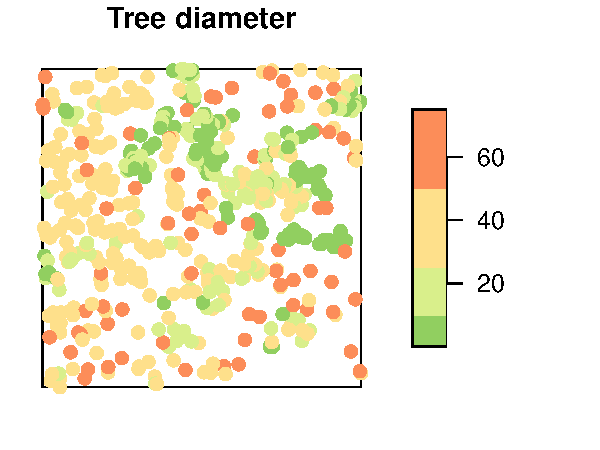
\includegraphics[keepaspectratio]{01_intro_files/figure-pdf/fig-longleaf_diam-1.pdf}}

}

\caption{\label{fig-longleaf_diam}Longleaf pine locations classified by
tree diameter. Data source: spatstat (Baddeley et al. 2016).}

\end{figure}%

Maps are ubiquitous. We encounter them online, in books, newspapers, and
countless mobile applications. Yet we rarely stop to consider how the
features shown on a map are represented within a computer. If software
is expected to analyze spatial data, then the location and shape of
geographic features must be stored in a form that the computer can
access and manipulate.

In the tree example, each observation can be represented by a pair of
coordinates, such as X and Y values (or longitude and latitude
coordinates). These coordinate pairs can be stored alongside the tree
attributes in a simple two-dimensional table.

{

\begin{longtable}[]{@{}ccc@{}}

\caption{\label{tbl-tree_table}Table showing the first few tree records.
Note the coordinate pairs stored as X and Y variables.}

\tabularnewline

\toprule\noalign{}
Diameter & X & Y \\
\midrule\noalign{}
\endhead
\bottomrule\noalign{}
\endlastfoot
32.9 & 200.0 & 8.8 \\
53.5 & 199.3 & 10.0 \\
68.0 & 193.6 & 22.4 \\
17.7 & 167.7 & 35.6 \\
36.9 & 183.9 & 45.4 \\
51.6 & 182.5 & 47.2 \\

\end{longtable}

}

A point is the simplest geographic feature to represent digitally
because each observation is defined by a single coordinate pair. More
complex features, however, require additional data structure. For
example, county boundaries enclose areas and are therefore represented
as polygons. A polygon is defined by a sequence of points, commonly
called \emph{vertices}, that together trace the feature's boundary.

\begin{figure}[H]

\centering{

\pandocbounded{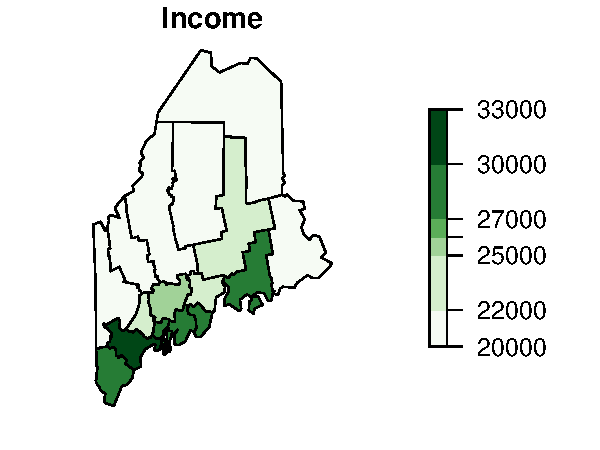
\includegraphics[keepaspectratio]{01_intro_files/figure-pdf/fig-me_income_couty-1.pdf}}

}

\caption{\label{fig-me_income_couty}Income data aggregate at the county
level. County feature are stored as polygons.}

\end{figure}%

Each county in the map above is represented by many vertices connected
to form a closed boundary. In addition, each county has associated
attributes, such as its median income. How should these coordinate
values be stored? How should the income attribute be linked to the
correct county and how can the software efficiently retrieve and analyze
this information?

These questions reveal the limitations of ordinary spreadsheets for
representing geographic features. While a spreadsheet can easily store a
few coordinate pairs, it provides no inherent mechanism for describing
complex geometries or maintaining the relationships between spatial
features and their attributes.

A GIS addresses this challenge through specialized data structures and
databases designed specifically for geographic information. These
systems store not only attribute values, but also the locations, shapes,
and spatial relationships of features such as points, lines, and
polygons. Although this may seem like a technical detail, it is the
foundation upon which spatial visualization, exploration, and analysis
are built.

\subsection{GIS software}\label{gis-software}

Many GIS software applications are available, both commercial and open
source. Two popular applications are \textbf{ArcGIS Pro} and
\textbf{QGIS}.

\subsubsection{ArcGIS Pro}\label{arcgis-pro}

A popular commercial desktop GIS software is
\href{https://www.esri.com/en-us/arcgis/products/arcgis-pro/overview}{ArcGIS
Pro} developed by \href{https://en.wikipedia.org/wiki/Esri}{Esri}
(pronounced \emph{ez-ree}). Esri was once a small land-use consulting
firm which did not start developing GIS software until the mid 1970s.
The software is available through several licensing options and can be
extended with specialized add-on products for applications such as 3D
analysis, image processing, and network modeling. A limitation for some
users is that ArcGIS Pro is designed primarily for Windows operating
systems.

\subsubsection{QGIS}\label{qgis}

A popular open-source alternative is \href{http://qgis.org}{QGIS}. It is
a free and cross-platform GIS application that runs on Windows, macOS,
and Linux. QGIS also provides access to tools from several open-source
GIS projects, including \href{https://grass.osgeo.org/}{GRASS GIS}.
GRASS has been under development since the 1980s and contains a large
collection of advanced geospatial analysis and data-processing tools.
While GRASS can be used as a stand-alone application, many users access
its functionality through the more user-friendly QGIS interface.

\section{What is Spatial Analysis?}\label{what-is-spatial-analysis}

A distinction is made in this course between \textbf{GIS} and
\textbf{spatial analysis}. GIS focuses primarily on the storage,
management, visualization, and manipulation of spatial data. Spatial
analysis, on the other hand, focuses on understanding and explaining
spatial patterns using quantitative and statistical methods.

In many GIS applications, the term \emph{analysis} often refers to
operations such as data processing, querying, overlay analysis,
buffering, and spatial data manipulation. In this course, however,
\emph{spatial analysis} refers more specifically to the statistical
examination of spatial patterns and the processes that may have
generated them.

In the previous tree-diameter example, we may wish to draw inferences
about the observed spatial pattern. Are large-diameter trees clustered
or dispersed? Is tree density consistent throughout the study area?
Could environmental factors such as soil type, slope, or moisture
availability have influenced the observed distribution? These are the
kinds of questions addressed through \emph{spatial analysis} using
quantitative and statistical techniques to explore and explain spatial
patterns.

In this course, you'll learn that software such as ArcGIS Pro and QGIS
excel at creating, visualizing, and managing spatial data. However, when
the goal is to conduct more advanced statistical analyses of spatial
patterns and processes, researchers often turn to specialized
quantitative tools. One such tool is \textbf{R}, a free and open-source
statistical computing environment.

R offers one of the richest collections of spatial analysis and
statistical packages available today. In addition to providing powerful
analytical capabilities, R promotes a reproducible workflow in which
data preparation, analysis, visualization, and reporting can be
documented in a single script. Many of the skills learned in R are
transferable to a wide range of quantitative analyses, both spatial and
non-spatial.

\href{http://www.r-project.org/}{R} can be installed on both Windows and
Mac operating systems. Another related piece of software that you might
find useful is
\href{https://posit.co/download/rstudio-desktop/}{RStudio} which offers
a nice interface to R. To learn more about data analysis in R, visit the
\href{http://mgimond.github.io/ES218/}{ES218 course website}.

\section{What's in an Acronym?}\label{whats-in-an-acronym}

GIS is a ubiquitous technology. Many of you are taking this course in
part because you have seen GIS listed as a \emph{desirable} or
\emph{required} skill in job postings. Often, GIS is viewed primarily as
a map-making tool, a perception shared by many casual users in the
workforce. While visualizing data is certainly an important function of
GIS, it is equally important to consider \emph{what} data is being
visualized and \emph{why} they are being mapped.

O'Sullivan and Unwin (O'Sullivan and Unwin 2010) use the term
\textbf{accidental geographer} to describe individuals \emph{``whose
understanding of geographic science is based on the operations made
possible by GIS software''}. Building on this idea, we introduce the
term \textbf{accidental data analyst}--someone whose grasp of data and
its analysis is limited to the point-and-click functionality of familiar
software such as spreadsheets, statistical packages, and GIS platforms.

This observation is not unique to GIS. Similar concerns arose when
personal computers made it easy to generate graphs, perform statistical
analyses, and produce polished reports with little understanding of the
underlying concepts. Software can make sophisticated tools widely
accessible, but it cannot replace an understanding of the questions
being asked or the assumptions underlying the analysis.

The different purposes of mapping spatial data closely parallel the
goals of graphing non-spatial data. \textbf{John Tukey} (Tukey 1972)
identified three broad categories of graphical displays:

\begin{itemize}
\tightlist
\item
  ``\emph{Graphs from which numbers are to be read off--substitutes for
  tables.}
\item
  \emph{Graphs intended to show the reader what has already been learned
  (by some other technique)--these we shall sometimes impolitely call
  propaganda graphs.}
\item
  \emph{Graphs intended to let us see what may be happening over and
  above what we have already described- these are the analytical graphs
  that are our main topic.}''
\end{itemize}

A GIS-based analogy to Tukey's categories might be:

\begin{itemize}
\tightlist
\item
  \textbf{Reference maps} (e.g., topographic maps, hiking maps, road
  maps): designed primarely to navigate landscapes or identify locations
  of interest.
\item
  \textbf{Presentation maps}: designed to convey a specific narrative.
  These maps emphasize clarity and effective communication and are often
  used in reports, news articles, and public presentations. Although we
  avoid Tukey's term ``propaganda,'' it's worth noting that maps can be
  powerful tools of persuasion.
\item
  \textbf{Statistical maps}: designed to explore spatial data in ways
  that reveal patterns. Such maps often involve transforming,
  summarizing, or modeling data to reveal relationships that would be
  difficult to detect in a table of raw observations.
\end{itemize}

This course emphasizes the latter two categories. Our goal is not simply
to produce attractive maps, but to use spatial data as a means of asking
and answering scientific questions about spatial relationships, spatial
patterns, and the processes that generate the observed patterns.

\section{Course Roadmap}\label{course-roadmap}

This course is divided into two main parts, each focusing on distinct
aspects of spatial data science.

\subsection{Part 1: Working with Spatial
Data}\label{part-1-working-with-spatial-data}

This section introduces foundational GIS concepts and tools for data
manipulation and visualization.

\begin{enumerate}
\def\labelenumi{\arabic{enumi}.}
\tightlist
\item
  \textbf{Introduction to GIS \& Spatial Analysis}

  \begin{itemize}
  \tightlist
  \item
    What is GIS?
  \item
    What is spatial analysis?
  \item
    GIS software overview
  \end{itemize}
\item
  \textbf{Feature Representation}

  \begin{itemize}
  \tightlist
  \item
    Vector vs.~Raster
  \item
    Object vs.~Field views
  \item
    Scale and attribute tables
  \end{itemize}
\item
  \textbf{GIS Data Management}

  \begin{itemize}
  \tightlist
  \item
    File formats and project organization
  \item
    Managing data in ArcGIS
  \end{itemize}
\item
  \textbf{Symbolizing Features}

  \begin{itemize}
  \tightlist
  \item
    Color theory and classification
  \item
    Choropleth mapping techniques
  \end{itemize}
\item
  \textbf{Statistical Maps}

  \begin{itemize}
  \tightlist
  \item
    Mapping distributions and uncertainty
  \item
    Classification intervals and outlier detection
  \end{itemize}
\item
  \textbf{Pitfalls to Avoid}

  \begin{itemize}
  \tightlist
  \item
    MAUP, ecological fallacy, unstable rates
  \end{itemize}
\item
  \textbf{Good Map Making Tips}

  \begin{itemize}
  \tightlist
  \item
    Map elements, layout, and typography
  \end{itemize}
\item
  \textbf{Spatial Operations and Vector Overlays}

  \begin{itemize}
  \tightlist
  \item
    Selection, overlays, and spatial queries
  \end{itemize}
\item
  \textbf{Coordinate Systems}

  \begin{itemize}
  \tightlist
  \item
    Geographic vs.~projected systems
  \item
    Spatial properties and geodesic geometries
  \end{itemize}
\item
  \textbf{Map Algebra}

  \begin{itemize}
  \tightlist
  \item
    Local, focal, zonal, and global raster operations
  \end{itemize}
\end{enumerate}

\subsection{Part 2: Spatial Analysis}\label{part-2-spatial-analysis}

This section focuses on statistical analysis of spatial patterns.

\begin{enumerate}
\def\labelenumi{\arabic{enumi}.}
\setcounter{enumi}{11}
\tightlist
\item
  \textbf{Spatial Trends}

  \begin{itemize}
  \tightlist
  \item
    First order analysis of field variables
  \item
    Fitting polynomial models
  \end{itemize}
\item
  \textbf{Spatial Autocorrelation}

  \begin{itemize}
  \tightlist
  \item
    Second order property of field variables
  \item
    Global and local Moran's I
  \end{itemize}
\item
  \textbf{Point Pattern Analysis: First order analysis}

  \begin{itemize}
  \tightlist
  \item
    Density and distance-based methods
  \item
    Testing for CSR processes
  \end{itemize}
\item
  \textbf{Point Pattern Analysis: Second order analysis}

  \begin{itemize}
  \tightlist
  \item
    ANN analysis
  \item
    K and L functions
  \item
    Paired correlation function
  \end{itemize}
\item
  \textbf{Spatial Interpolation}

  \begin{itemize}
  \tightlist
  \item
    Deterministic (IDW, Thiessen) and statistical (Kriging) methods
  \end{itemize}
\end{enumerate}

\part{Working with Spatial Data}

\chapter{Feature Representation}\label{feature-representation}

\section{Introduction}\label{introduction-1}

Before we can analyze or visualize spatial data in a GIS, we must first
decide how to represent real-world phenomena in a digital environment.
This chapter introduces the foundational data models used in
GIS--\textbf{vector} and \textbf{raster}--and explores how different
types of geographic features are encoded using these models.
Understanding how features are represented is essential for making
informed decisions about data collection, storage, analysis, and
visualization.

We'll also examine conceptual frameworks such as the \textbf{object}
vs.~\textbf{field} view of the world, the role of scale in determining
how features are modeled, and how attribute data are structured and
classified. These concepts form the backbone of spatial data modeling
and are critical for interpreting and working with spatial data
effectively throughout the rest of the course.

\section{Vector vs.~Raster}\label{vector-vs.-raster}

To work in a GIS environment, real world observations (objects or events
that can be recorded in 2D or 3D space) need to be reduced to spatial
entities. These spatial entities can be represented in a GIS as a
\textbf{vector data model} or a \textbf{raster data model}.

\begin{figure}[H]

\centering{


\includegraphics[width=2.5in,height=\textheight,keepaspectratio]{img/vector_vs_raster.jpg}

}

\caption{\label{fig-vector_vs_raster}Vector and raster representations
of a river feature.}

\end{figure}%

\subsection{Vector}\label{vector}

Vector features can be decomposed into three different geometric
primitives: \textbf{points}, \textbf{polylines} and \textbf{polygons}.

Vector data models are used to represent discrete features like roads,
buildings and boundaries. They also benefit from supporting rich
attribute data and precise geometry.

Let's explore how different types of features are represented using the
vector model.

\subsubsection{Point}\label{point}

\begin{figure}[H]

\centering{

\pandocbounded{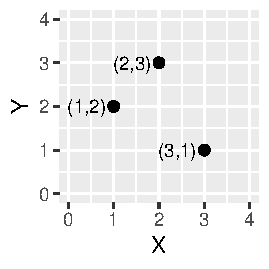
\includegraphics[keepaspectratio]{02_feature_representation_files/figure-pdf/fig-point-1.pdf}}

}

\caption{\label{fig-point}Three point objects defined by their X and Y
coordinate values.}

\end{figure}%

A \textbf{point} is composed of one coordinate pair representing a
specific location in a coordinate system. Points are the most basic
geometric primitives having no length or area. By definition a point
can't be ``seen'' since it has no area; but this is not practical if
such primitives are to be mapped. So points on a map are represented
using \emph{symbols} that have both area and shape (e.g.~circle, square,
plus signs).

We seem capable of interpreting such symbols as points, but there may be
instances when such interpretation may be ambiguous (e.g.~is a round
symbol delineating the area of a round feature on the ground such as a
large oil storage tank or is it representing the point location of that
tank?).

\subsubsection{Polyline}\label{polyline}

\begin{figure}[H]

\centering{

\pandocbounded{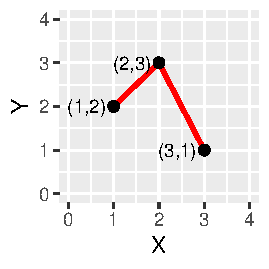
\includegraphics[keepaspectratio]{02_feature_representation_files/figure-pdf/fig-polyline-1.pdf}}

}

\caption{\label{fig-polyline}A simple polyline object defined by
connected vertices.}

\end{figure}%

A \textbf{polyline} is composed of a sequence of two or more coordinate
pairs called \textbf{vertices}. A vertex is defined by coordinate pairs,
just like a point, but what differentiates a vertex from a point is its
explicitly defined relationship with neighboring vertices. A vertex is
connected to at least one other vertex.

A polyline represents \textbf{length}. Like a point, a true line can't
be seen since it has no area. And like a point, a line is symbolized
using shapes that have a color, width and style (e.g.~solid, dashed,
dotted, etc\ldots). Roads and rivers are commonly stored as polylines in
a GIS.

\subsubsection{Polygon}\label{polygon}

\begin{figure}[H]

\centering{

\pandocbounded{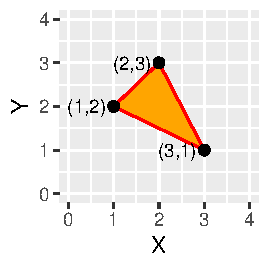
\includegraphics[keepaspectratio]{02_feature_representation_files/figure-pdf/fig-polygon-1.pdf}}

}

\caption{\label{fig-polygon}A simple polygon object defined by an area
enclosed by connected vertices.}

\end{figure}%

A \textbf{polygon} is composed of three or more line segments whose
starting and ending coordinate pairs are the same. Sometimes you will
see the words \emph{lattice} or \emph{area} used in lieu of
\emph{polygon}.

Polygons represent both \textbf{length} (i.e.~the perimeter of the area)
and \textbf{area}. They also embody the idea of an \emph{inside} and an
\emph{outside}; in fact, the area that a polygon encloses is explicitly
defined in a GIS environment. If it isn't, then you are working with a
polyline feature. If this does not seem intuitive, think of three
connected lines defining a triangle: they can represent three connected
road segments (thus polyline features), or they can represent the grassy
strip enclosed by the connected roads (in which case an `inside' is
implied thus defining a polygon).

\subsection{Raster}\label{raster}

\begin{figure}[H]

\centering{

\pandocbounded{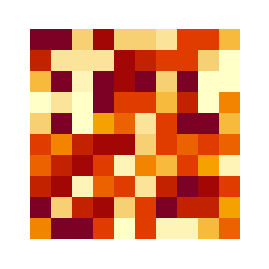
\includegraphics[keepaspectratio]{02_feature_representation_files/figure-pdf/fig-raster-1.pdf}}

}

\caption{\label{fig-raster}A simple raster object defined by a 10x10
array of cells or pixels.}

\end{figure}%

A \textbf{raster} data model uses an array of \textbf{cells}, or
\textbf{pixels}, to represent real-world objects. Raster datasets are
commonly used for representing and managing imagery, surface
temperatures, digital elevation models, and any other continuous data.

A raster can be thought of as a special case of an area object where the
area is divided into a regular grid of cells. While rasters are often
described as grids of cells, they can also be thought of as arrays of
spatially referenced values, each tied to a specific location in space.

In a raster data model, each cell (or pixel) is explicitly associated
with a value, representing a measurement or classification at that
location. This contrasts with the vector model, where attribute values
are linked to geometric features (points, lines, or polygons) and may
not be defined for every location in space.

Raster datasets are organized as regular grids that are typically square
in shape. If the spatial features of interest do not occupy the entire
extent of the grid, the remaining cells are assigned special values such
as \texttt{NULL} or \texttt{NoData} to indicate the absence of valid
data.

\section{Object vs.~Field}\label{object-vs.-field}

While the vector/raster distinction focuses on data structure, the
\textbf{object} vs.~\textbf{field} perspective focuses on how we
\textbf{conceptualize} spatial phenomena. This distinction is especially
useful when deciding how to model and analyze different types of spatial
features.

\subsection{Object View}\label{object-view}

The \textbf{object view} treats spatial features as discrete entities
that exist independently and occupy specific locations. These features
do not occur everywhere in space. Examples include point locations of
cities, road networks, or polygonal representations of land parcels or
urban areas. Objects are typically represented using the vector data
model.

\subsection{Field View}\label{field-view}

The \textbf{field view} treats spatial phenomena as \emph{continuous
surfaces} or distributions that vary across space. A field is a property
that can be measured at any location within a study area. Common
examples include surface elevation, temperature, or precipitation. These
are typically represented using the raster data model but can be
represented with polygons.

Some features can be represented as either \emph{objects} or
\emph{fields}, depending on the analytical context. For instance, the
presence or absence of buildings can be modeled as:

\begin{itemize}
\tightlist
\item
  \textbf{Objects}, if we are interested in the location and shape of
  individual buildings.
\item
  \textbf{Fields}, if we are interested in identifying areas where
  buildings do or do not exist (e.g., using a binary raster where 1 =
  presence, 0 = absence).
\end{itemize}

\begin{figure}[H]

\centering{

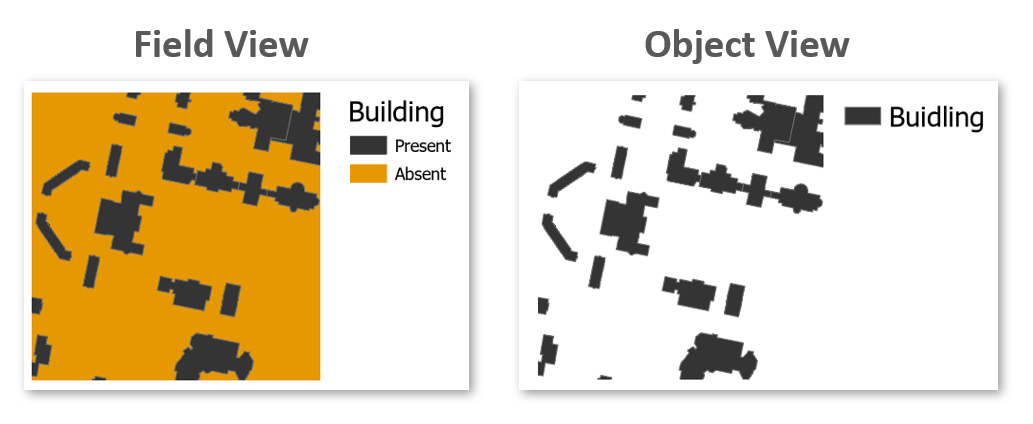
\includegraphics[width=4in,height=\textheight,keepaspectratio]{img/field_vs_object.png}

}

\caption{\label{fig-field_vs_object}Field and Object representation of
buildings.}

\end{figure}%

Ultimately, the choice between object and field representations depends
on the nature of the phenomenon and the goals of the analysis.

\section{Scale}\label{scale}

In GIS, \textbf{scale} refers to the ratio between a distance on the map
and the corresponding distance in the real world. For example, a scale
of 1:10,000 means that one unit on the map represents 10,000 units on
the ground.

It's important to distinguish between two uses of the term:

\begin{itemize}
\tightlist
\item
  \textbf{Cartographic scale} refers to the map's level of detail.
\item
  \textbf{Analytical scale} refers to the spatial extent or resolution
  of a study.
\end{itemize}

In cartographic terms, a \textbf{large scale} map (e.g., 1:10,000) shows
a small area in great detail, while a \textbf{small scale} map (e.g.,
1:10,000,000) shows a large area with less detail. This is opposite to
how \emph{``large scale''} is often used in everyday language, where it
implies a broad or extensive scope.

The following two maps of the Boston region illustrate this difference:

\begin{itemize}
\tightlist
\item
  At a small scale (1:10,000,000), Boston and other cities may be
  represented as simple points.
\item
  At a large scale (1:34,000), Boston may be represented as a detailed
  polygon, and roads may appear as polygons rather than simple lines.
\end{itemize}

\begin{figure}[H]

\centering{


\includegraphics[width=3.5in,height=\textheight,keepaspectratio]{img/Boston_small_scale.jpg}

}

\caption{\label{fig-small_scale}Map of the Boston area at a 1:10,000,000
scale. Note that in geography, this is considered small scale whereas in
layperson terms, this extent is often referred to as a large scale
(i.e.~covering a large area).}

\end{figure}%

\begin{figure}[H]

\centering{


\includegraphics[width=3.5in,height=\textheight,keepaspectratio]{img/Boston_large_scale.jpg}

}

\caption{\label{fig-large_scale}Map of the Boston area at a 1:34,000
scale. Note that in geography, this is considered large scale whereas in
layperson terms, this extent is often referred to as a small scale
(i.e.~covering a small area).}

\end{figure}%

Understanding scale is essential for choosing appropriate data and
representation methods in GIS analysis.

\section{Attribute Tables}\label{attribute-tables}

In GIS, \textbf{attributes} are non-spatial data that describe the
characteristics of spatial features such as a city's population, a
road's name, or a parcel's land use type. A feature on a GIS map is
linked to its record in the attribute table by a unique numerical
identifier (ID).

Each feature in a GIS layer is associated with one or more records in
the attribute table, enabling a \textbf{one-to-one} or
\textbf{many-to-one} relationship between geometry and descriptive data.
Most GIS software allows users to click on a map feature and view its
associated attributes directly.

Raster datasets also store \emph{attribute} information. In such case,
each unique integer value may correspond to a class label or description
if the attribute is categorical in nature. However, most raster datasets
used in this course will represent continuous data stored as an integer
or double.

\subsection{Measurement Levels}\label{measurement-levels}

Attribute data can be broken down into four \textbf{measurement levels}:

\begin{itemize}
\item
  \textbf{Nominal} data which have no implied order, size or
  quantitative information (e.g.~paved and unpaved roads)
\item
  \textbf{Ordinal} data have an implied order (e.g.~ranked scores),
  however, we cannot quantify the difference since a linear scale is not
  implied.
\item
  \textbf{Interval} data are numeric and have a linear scale, however
  they do not have a true zero and can therefore not be used to measure
  \emph{relative} magnitudes. For example, one cannot say that 60°F is
  twice as warm as 30°F since when presented in degrees °C the
  temperature values are 15.5°C and -1.1°C respectively (and 15.5 is
  clearly not twice as big as -1.1).
\item
  \textbf{Ratio} scale data are interval data with a true zero such as
  monetary value (e.g.~\$1, \$20, \$100).
\end{itemize}

\subsection{Data type}\label{data-type}

In GIS, choosing the correct \textbf{data type} for an attribute is
essential for accurate data storage, efficient processing, and
meaningful analysis. ArcGIS supports several common data types,
including \textbf{integer}, \textbf{float}, \textbf{double}, and
\textbf{text}. The choice of data type should align with the attribute's
measurement level and intended use.

The following table summarizes popular data types available in most GIS
applications:

{\def\LTcaptype{none} % do not increment counter
\begin{longtable}[]{@{}lll@{}}
\toprule\noalign{}
Type & Stored values & Note \\
\midrule\noalign{}
\endhead
\bottomrule\noalign{}
\endlastfoot
Short integer & -32,768 to 32,767 & Whole numbers \\
Long integer & -2,147,483,648 to 2,147,483,647 & Whole numbers \\
Float & -3.4 * E-38 to 1.2 E38 & Real numbers \\
Double & -2.2 * E-308 to 1.8 * E308 & Real numbers \\
Text & Up to 64,000 characters & Letters and words \\
\end{longtable}
}

While whole numbers can be stored as floats or doubles (e.g., storing 2
as 2.0), doing so increases storage requirements. This may not be a
concern for small datasets, but for large datasets with tens of
thousands of records, it can impact file size and processing speed.

Conversely, storing decimal values as integers can lead to significant
data loss. For example, values such as 0.2, 0.01, 0.34, 0.1, and 0.876
would all round to either 0 or 1, obscuring meaningful differences. This
can distort map outputs, especially in choropleth visualizations, where
subtle variations are important as shown in the following two figures.

\begin{figure}[H]

\centering{

\pandocbounded{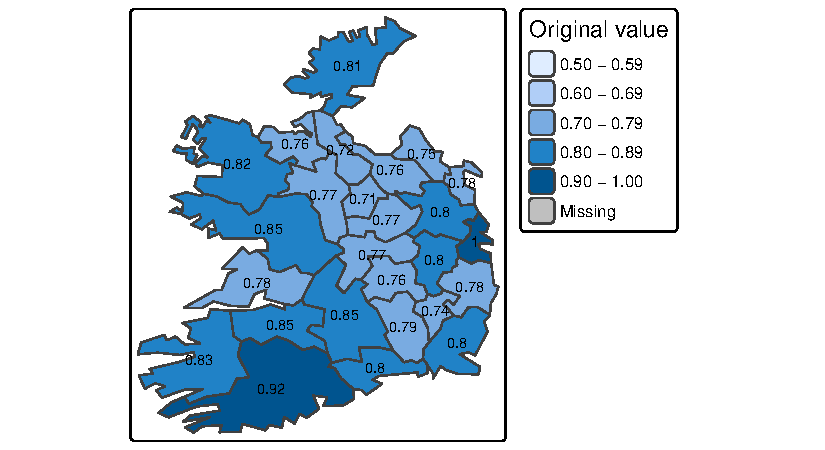
\includegraphics[keepaspectratio]{02_feature_representation_files/figure-pdf/fig-decimal_data-1.pdf}}

}

\caption{\label{fig-decimal_data}Map of data represented as decimal
(float) values. Data source: spData package (Bivand et al. 2026)}

\end{figure}%

\begin{figure}[H]

\centering{

\pandocbounded{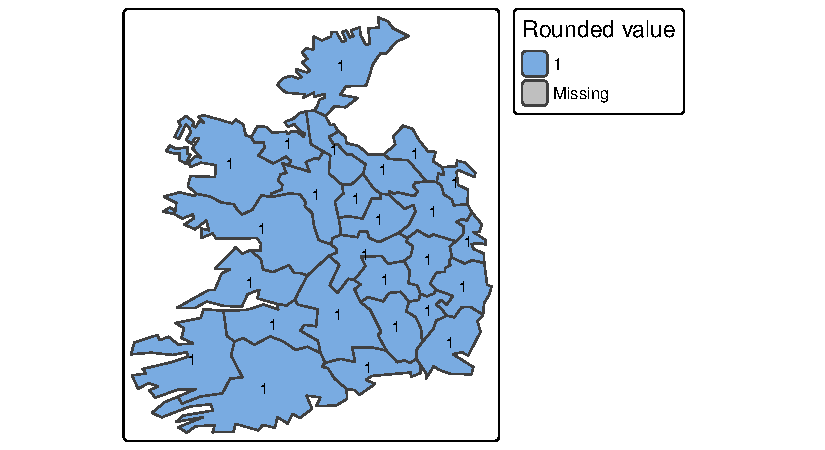
\includegraphics[keepaspectratio]{02_feature_representation_files/figure-pdf/fig-integer_data-1.pdf}}

}

\caption{\label{fig-integer_data}Map of same data represented as
integers instead of float. Data source: spData package (Bivand et al.
2026)}

\end{figure}%

\section{Summary}\label{summary}

This chapter introduces the foundational concepts of how geographic
features are represented in a GIS environment. It begins by
distinguishing between the two primary data models--\emph{vector} and
\emph{raster}--and explains how real-world entities are encoded as
points, lines, polygons, or grids of cells.

The discussion then shifts to conceptual frameworks, including the
object vs.~field view of spatial phenomena, which helps clarify how the
same feature can be represented differently depending on the analytical
context. The importance of scale is also addressed, with a focus on how
map detail and spatial extent influence representation choices.

Finally, the chapter explores attribute tables, which store non-spatial
information linked to spatial features, and introduces key concepts such
as measurement levels (nominal, ordinal, interval, ratio) and data types
(integer, float, double, text). These distinctions are critical for
ensuring accurate data storage, querying, and analysis in GIS workflows.

\chapter{GIS Data Management}\label{gis-data-management}

\section{Introduction}\label{introduction-2}

Effective data management is essential to any GIS workflow. Whether
working with spatial data for analysis, visualization, or sharing,
understanding how GIS files are structured, stored, and organized
ensures efficiency, and reproducibility. This chapter introduces the
most common GIS file formats used for both vector and raster data,
highlighting their strengths, limitations, and compatibility across
platforms.

Beyond file formats, the chapter explores best practices for managing
GIS projects within software environments like ArcGIS. Topics such
project folder organization and file dependencies are covered to help
avoid common pitfalls when working with complex spatial datasets.

\section{GIS File Data Formats}\label{gis-file-data-formats}

Imagine you download a roads layer from a state GIS office, a land-cover
raster from the USGS, and create your own points in a GIS software. Why
do some datasets appear as a single file while others appear as folders
containing dozens of files? Why do some layers work in ArcGIS Pro but
not others? Why do projects sometimes open with broken links?
Understanding GIS data formats and project organization helps answer
these questions.

In the GIS world, you will encounter many different GIS file formats.
Some file formats are unique to specific GIS applications, others are
universal. For this course, we will focus on a subset of spatial data
file formats: \textbf{shapefiles} for vector data, \textbf{Imagine} and
\textbf{GeoTiff} files for rasters and \textbf{file geodatabases} and
\textbf{GeoPackages} for both vector and raster data.

\section{Comparison table}\label{comparison-table}

The following table summarizes key characteristics of the most commonly
used GIS file formats discussed above. This comparison includes aspects
such as data type, structure, portability, and support for topology and
metadata. Metadata are ``data about data'' and can include information
such as the dataset creator, date of creation, coordinate system,
source, and processing history.

\begin{longtable}[]{@{}
  >{\raggedright\arraybackslash}p{(\linewidth - 12\tabcolsep) * \real{0.1389}}
  >{\raggedright\arraybackslash}p{(\linewidth - 12\tabcolsep) * \real{0.1389}}
  >{\raggedright\arraybackslash}p{(\linewidth - 12\tabcolsep) * \real{0.1389}}
  >{\raggedright\arraybackslash}p{(\linewidth - 12\tabcolsep) * \real{0.1389}}
  >{\raggedright\arraybackslash}p{(\linewidth - 12\tabcolsep) * \real{0.1389}}
  >{\raggedright\arraybackslash}p{(\linewidth - 12\tabcolsep) * \real{0.1389}}
  >{\raggedright\arraybackslash}p{(\linewidth - 12\tabcolsep) * \real{0.1667}}@{}}
\caption{Common GIS Data Formats}\label{tbl-formats}\tabularnewline
\toprule\noalign{}
\begin{minipage}[b]{\linewidth}\raggedright
Format
\end{minipage} & \begin{minipage}[b]{\linewidth}\raggedright
Type
\end{minipage} & \begin{minipage}[b]{\linewidth}\raggedright
Structure
\end{minipage} & \begin{minipage}[b]{\linewidth}\raggedright
Portability
\end{minipage} & \begin{minipage}[b]{\linewidth}\raggedright
Topology Support
\end{minipage} & \begin{minipage}[b]{\linewidth}\raggedright
Metadata Support
\end{minipage} & \begin{minipage}[b]{\linewidth}\raggedright
Notes
\end{minipage} \\
\midrule\noalign{}
\endfirsthead
\toprule\noalign{}
\begin{minipage}[b]{\linewidth}\raggedright
Format
\end{minipage} & \begin{minipage}[b]{\linewidth}\raggedright
Type
\end{minipage} & \begin{minipage}[b]{\linewidth}\raggedright
Structure
\end{minipage} & \begin{minipage}[b]{\linewidth}\raggedright
Portability
\end{minipage} & \begin{minipage}[b]{\linewidth}\raggedright
Topology Support
\end{minipage} & \begin{minipage}[b]{\linewidth}\raggedright
Metadata Support
\end{minipage} & \begin{minipage}[b]{\linewidth}\raggedright
Notes
\end{minipage} \\
\midrule\noalign{}
\endhead
\bottomrule\noalign{}
\endlastfoot
Shapefile & Vector & Multi-file & High & No & Limited & Legacy format,
widely supported \\
File Geodatabase & Vector/Raster & Folder-based & Low (ESRI only) & Yes
& Strong & Efficient for large datasets \\
GeoPackage & Vector/Raster & Single file & High & Partial & Strong &
Open format, cross-platform \\
Imagine (.img) & Raster & Single file (+xml) & Medium & N/A & Moderate &
Common in remote sensing \\
GeoTIFF & Raster & Single file & High & N/A & Strong & Public domain,
widely supported \\
\end{longtable}

\section{Vector Data File Formats}\label{vector-data-file-formats}

\subsection{Shapefile}\label{shapefile}

A \textbf{shapefile} is a file-based data format native to ArcView 3.x
software (a much older version of ArcGIS Pro). Conceptually, a shapefile
is a feature class--it stores a collection of features that have the
same geometry type (point, line, or polygon), attributes, and spatial
extent.

Despite its name, a shapefile is not a single file but a set of files
that work together. At minimum, three files are required, but up to
eight may be present. Each file shares the same base name but has a
different extension, as shown below:

{\def\LTcaptype{none} % do not increment counter
\begin{longtable}[]{@{}ll@{}}
\toprule\noalign{}
File extension & Content \\
\midrule\noalign{}
\endhead
\bottomrule\noalign{}
\endlastfoot
.dbf & Attribute information \\
.shp & Feature geometry \\
.shx & Feature geometry index \\
.aih & Attribute index \\
.ain & Attribute index \\
.prj & Coordinate system information \\
.sbn & Spatial index file (optional) \\
.sbx & Spatial index file (optional) \\
\end{longtable}
}

While shapefiles are widely supported and simple to use, they have
notable limitations, such as lack of support for topology, limited
attribute field name lengths, and constraints on file size and data
types.

\subsection{File Geodatabase}\label{file-geodatabase}

A \textbf{file geodatabase} is a relational database storage format
developed by Esri. It is a more complex and versatile structure than the
shapefile, consisting of a \textbf{.gdb} folder that houses dozens of
files. These files collectively store spatial features, attribute
tables, indexes, metadata, and rules that define relationships between
features.

One of the key advantages of a file geodatabase is its ability to store
multiple feature classes (e.g.~vector layers) and raster datasets within
a single container. It also supports topological rules, which allow
users to define spatial relationships between features---such as shared
boundaries or connectivity between lines.

An example of a geodatabase's contents is shown in the following figure.

\begin{figure}[H]

\centering{

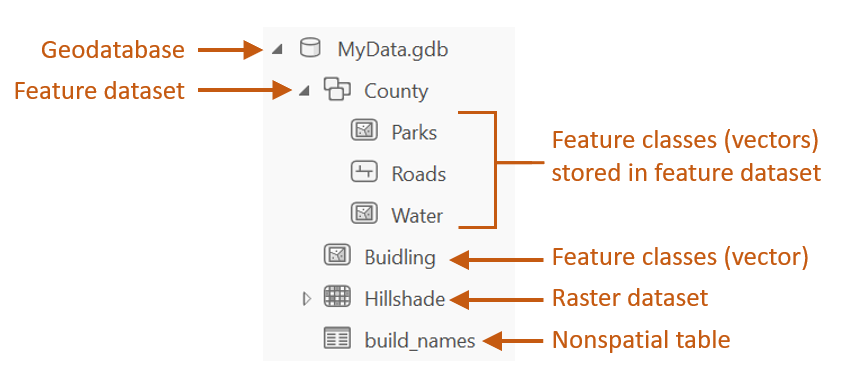
\includegraphics[width=4in,height=\textheight,keepaspectratio]{img/geodatabase.png}

}

\caption{\label{fig-geodatabase}Sample content of an ArcGIS file
geodatabase.}

\end{figure}%

File geodatabases are efficient for managing large datasets and support
advanced GIS operations. However, they are proprietary to ESRI and may
have limited compatibility with non-ESRI software.

\subsection{GeoPackage}\label{geopackage}

A \textbf{GeoPackage} is a modern, open-standard data format built on
top of SQLite--a lightweight, self-contained relational database. It is
\href{https://www.geopackage.org/}{non-proprietary} and designed for
efficient storage and transfer of spatial data. One of its key
advantages is compactness: coordinate values, metadata, attribute
tables, projection information, and even multiple layers (vector and
raster) can be stored in a single .gpkg file.

This structure makes GeoPackage highly portable and ideal for sharing
complex GIS projects. Unlike shapefiles, which require multiple files,
or file geodatabases, which are proprietary to Esri, GeoPackage offers a
unified and open solution compatible with a wide range of applications
including QGIS (2.12 and up), R, and ArcGIS Pro.

An example of a GeoPackage's contents is shown in the following figure.

\begin{figure}[H]

\centering{

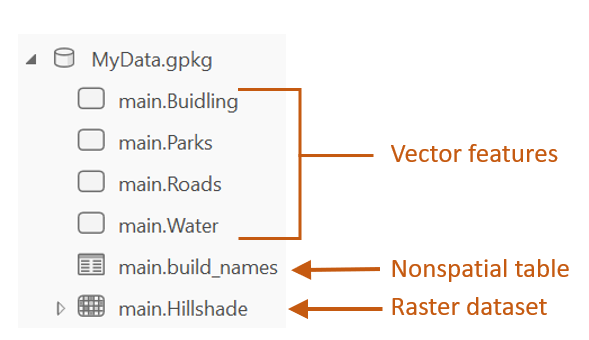
\includegraphics[width=3in,height=\textheight,keepaspectratio]{img/geopackage.png}

}

\caption{\label{fig-geopackage}Sample content of a GeoPackage.}

\end{figure}%

While GeoPackage supports many advanced features, performance may vary
depending on the software and dataset size. Some specialized
capabilities, such as topology rules, may be more limited compared to
Esri's file geodatabase.

\section{Raster Data File Formats}\label{raster-data-file-formats}

Raster data represents spatial phenomena as a grid of cells (pixels),
each storing a numeric value. These values can represent elevation,
temperature, and land cover for example. Rasters are particularly
well-suited for modeling continuous surfaces and are commonly used in
remote sensing and environmental analysis.

Some of the most popular raster file formats are listed next

\subsection{Imagine}\label{imagine}

The \textbf{Imagine} file format was originally created by an image
processing software company called ERDAS. This file format consists of a
single \textbf{.img} file. This is a simpler file format than the vector
shapefile. It is sometimes accompanied by an .xml file which usually
stores metadata information about the raster layer.

\subsection{GeoTiff}\label{geotiff}

A popular public domain raster data format is the \textbf{GeoTIFF}
format. It extends the standard TIFF (Tagged Image File Format) by
embedding georeferencing information directly within the file. This
includes coordinate system, projection, datum, and spatial resolution,
allowing the raster to be accurately placed in geographic space without
the need for auxiliary files.

GeoTIFF is widely supported across GIS and remote sensing software,
including QGIS, ArcGIS and R. Its portability, platform independence,
and open specification make it a popular format for sharing raster data.

GeoTIFF also supports internal compression (e.g., LZW, DEFLATE, JPEG),
which can reduce file size.

\subsection{File Geodatabase}\label{file-geodatabase-1}

A raster file can also be stored in a file geodatabase alongside vector
files. Geodatabases have the benefit of defining image mosaic structures
thus allowing the user to create ``stitched'' images from multiple image
files stored in the geodatabase. Also, processing very large raster
files can be computationally more efficient when stored in a file
geodatabase as opposed to an Imagine or GeoTiff file format.

\subsection{GeoPackage}\label{geopackage-1}

In addition to vector data, GeoPackage also supports raster data
storage. Raster layers are stored in a tiled format within the same
.gpkg file making it a compact and portable solution for mixed data
types. GeoPackage is a good choice for sharing raster data across
platforms due to its open standard and single-file structure.

\section{A Note About Raster Pixel
Depth}\label{a-note-about-raster-pixel-depth}

Thus far we have focused on how raster data are stored. Another
important characteristic of raster datasets is how cell values
themselves are encoded. In raster data, \textbf{pixel depth} (aka
\textbf{bit depth}) refers to the number of bits used to store the value
of each pixel (cell). It determines the range and precision of values
that can be represented. The choice of pixel depth also affects raster
file size, storage requirements, and processing efficiency, as rasters
with greater bit depths require more memory and disk space.

For example, a 1-bit raster can only store two values (0 and 1), while a
16-bit raster can store up to 65,536 distinct values. The following
figure illustrates how pixel depth affects the range of values.

\begin{figure}[H]

\centering{

\pandocbounded{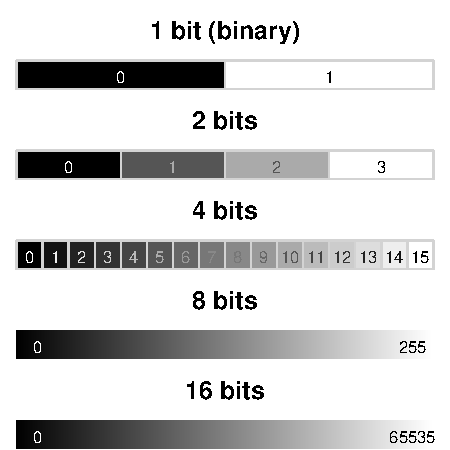
\includegraphics[keepaspectratio]{03_data_management_files/figure-pdf/fig-pixeldepth-1.pdf}}

}

\caption{\label{fig-pixeldepth}Increasing pixel depth increases the
number of possible pixel values and corresponding gray levels that can
be represented in a raster, from 2 values in a 1-bit raster to 65,536
values in a 16-bit raster.}

\end{figure}%

\section{Managing GIS Files in
ArcGIS}\label{managing-gis-files-in-arcgis}

Due to the complex and often multi-file structure of many GIS
formats--such as shapefiles or file geodatabases--it is strongly
recommended to manage GIS files (e.g., copy, move, delete, rename) from
within the GIS software environment rather than through external tools
like Windows File Explorer. GIS applications are designed to handle the
internal dependencies and metadata links that exist between files.

Managing files outside of GIS software can lead to broken links, missing
components, or corrupted datasets, especially when dealing with formats
that span multiple files or folders. For example, a shapefile may appear
as a single layer in ArcGIS but is actually composed of several
interdependent files. Renaming or moving just one of these files
manually can render the entire dataset unusable.

The figure below illustrates how ArcGIS Catalog simplifies file
management by presenting complex datasets as unified entries, reducing
the risk of accidental mismanagement.

\begin{figure}[H]

\centering{


\includegraphics[width=1\linewidth,height=\textheight,keepaspectratio]{img/ArcCatalog.jpg}

}

\caption{\label{fig-catalog}Windows File Explorer view vs.~ArcGIS
Catalog view. Note, for example, how the many files that make up the
Cities shapefile (as viewed in a Windows file manager environment)
appears as a single entry in the Catalog view. This makes it easier to
rename the shapefile in ArcGIS since it needs to be done only for a
single entry in the GIS software (as opposed to renaming the Cities
files seven times in the Windows file manager environment).}

\end{figure}%

\section{Managing GIS Projects and File
References}\label{managing-gis-projects-and-file-references}

Unlike many other software environments--such as word processors or
spreadsheets--a GIS project is not self-contained in a single file.
Instead, it consists of a project file (e.g., \texttt{.aprx} in ArcGIS
Pro or \texttt{.qgz} in QGIS) and a collection of external spatial data
files (e.g., shapefiles, rasters, geodatabases, or GeoPackages). The
project file stores information about how layers are symbolized and
where the associated data files are located, but it does not embed the
data itself.

Because of this structure, GIS software must be able to locate the
external data files referenced in the project. If any of these files are
renamed, moved, or deleted outside of the GIS environment (e.g., using
\emph{Windows' File Explorer}), the project file may no longer be able
to find them. This results in \textbf{broken links}, which prevent the
layers from loading properly.

In ArcGIS Pro, broken links are indicated by \textbf{exclamation marks}
next to the affected layers in the \emph{Contents} pane. This typically
occurs when the file path stored in the project no longer matches the
actual location of the data on disk.

\begin{figure}[H]

\centering{

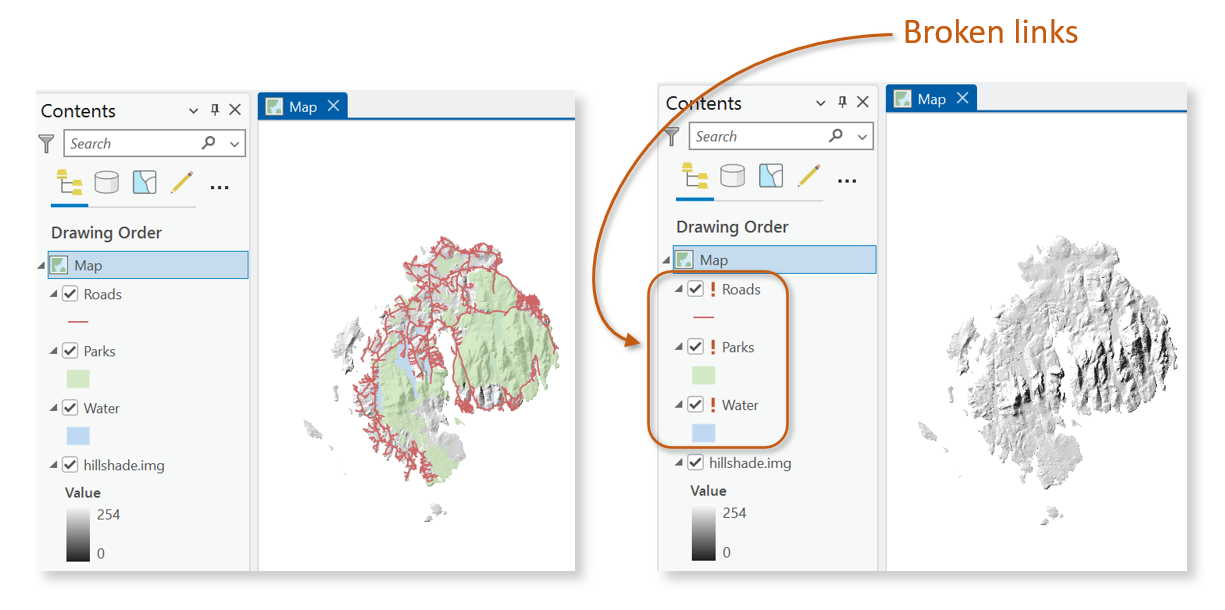
\includegraphics[width=6in,height=\textheight,keepaspectratio]{img/Exclamation_marks.png}

}

\caption{\label{fig-exclamation}Figure shows an ArcGIS Pro project with
properly referenced GIS layers (left) and the same project reopened
after the associated data files were moved or deleted outside of ArcGIS
(right). The broken links are indicated by exclamation marks next to the
affected layers, signaling that the project can no longer locate the
original data sources.}

\end{figure}%

To avoid these issues, it is best practice to:

\begin{itemize}
\tightlist
\item
  Keep all project-related files in a single, well-organized folder.
\item
  Use \textbf{relative pathnames}, which store file locations relative
  to the project file's location rather than as full absolute paths.
\item
  Avoid renaming, moving, or deleting GIS data files outside of the GIS
  software.
\end{itemize}

\section{Summary}\label{summary-1}

This chapter introduced the fundamentals of GIS data management and
organization.

\begin{itemize}
\tightlist
\item
  GIS data are stored in a variety of formats, including
  \textbf{shapefiles}, \textbf{file geodatabases}, \textbf{GeoPackages},
  \textbf{GeoTIFFs}, and \textbf{Imagine} files. Each format has
  advantages and limitations.
\item
  Shapefiles are widely supported but consist of multiple files, whereas
  GeoPackages store spatial data in a single portable file and file
  geodatabases support advanced GIS capabilities.
\item
  Raster datasets can be stored in several formats, and \textbf{pixel
  depth} determines the range and precision of values that a raster can
  represent.
\item
  GIS data should be managed from within the GIS software environment to
  avoid breaking internal file dependencies.
\item
  GIS projects store references to data files rather than the data
  themselves, making folder organization and file management critical.
\item
  Using consistent folder structures and avoiding unnecessary file moves
  or renaming helps ensure that GIS projects remain functional and
  reproducible.
\end{itemize}

Understanding GIS file formats and project organization is an important
foundation for efficient GIS workflows and successful spatial analysis.

\chapter{Symbolizing features}\label{symbolizing-features}

\section{Introduction}\label{introduction-3}

Effective map design is not just about placing data on a map, it's about
communicating information clearly and accurately. This chapter explores
the principles and practices behind symbolizing spatial features,
focusing on how color and classification schemes can be used to enhance
the readability and interpretability of maps.

The chapter begins by breaking down the three perceptual dimensions of
color--\textbf{hue}, \textbf{lightness}, and \textbf{saturation}--and
explains how each can be used to represent different types of data. It
then introduces the concept of color spaces, including the commonly used
HSV (Hue-Saturation-Value) model and perceptually accurate models like
CIELAB and Munsell, highlighting how human perception of color can
differ from software-generated color models.

The chapter also covers classification schemes used in choropleth
mapping:

\begin{itemize}
\tightlist
\item
  \textbf{Qualitative} schemes for categorical data,
\item
  \textbf{Sequential} schemes for ordered data,
\item
  \textbf{Divergent} schemes for data with a meaningful midpoint.
\end{itemize}

It emphasizes the importance of choosing appropriate classification
intervals, such as \textbf{equal interval}, \textbf{quantile}, and
\textbf{Jenks natural breaks}, and demonstrates how different choices
can significantly affect the appearance and interpretation of a map.

Finally, the chapter introduces tools like ColorBrewer, which help
cartographers select color palettes that are visually effective,
colorblind-safe, and suitable for grayscale printing.

\section{Color}\label{color}

Color plays a central role in map design, influencing how effectively
spatial patterns and relationships are communicated. In cartography,
color is not just aesthetic--it encodes meaning and guides
interpretation. To use color effectively, it's important to understand
its three perceptual dimensions: \textbf{hue}, \textbf{lightness} and
\textbf{saturation}. These dimensions interact to shape how we perceive
and differentiate features on a map. In the following sections, we'll
explore each dimension and its implications for symbolizing different
types of data.

\subsection{Hue}\label{hue}

\textbf{Hue} is the perceptual dimension most commonly associated with
color names--such as red, green, or blue. In cartography, hue is
typically used to represent \textbf{categorical} data, where each
category is assigned a distinct color. This allows map readers to easily
differentiate between classes without implying any order or magnitude.
However, the choice of hues should be made carefully, as some colors may
carry cultural connotations or be difficult to distinguish for
individuals with color vision deficiencies.

\begin{figure}[H]

\centering{

\pandocbounded{
\includegraphics[keepaspectratio]{04_symbolizing_features_files/figure-pdf/fig-hue-1.pdf}}

}

\caption{\label{fig-hue}An example of eight different hues. Hues are
associated with color names such as green, red or blue.}

\end{figure}%

Note that magentas and purples are not part of the natural visible light
spectrum; instead they are a mix of reds and blues (or violets) from the
spectrum's tail ends.

\subsection{Lightness}\label{lightness}

\textbf{Lightness}--sometimes referred to as \textbf{value}--describes
how much light is reflected or emitted from a surface, influencing how
bright or dark a color appears. In cartographic design, lightness is
particularly useful for symbolizing \textbf{ordinal}, \textbf{interval},
or \textbf{ratio} data (i.e., data that have a meaningful ordering or
numeric scale), where a progression from light to dark can intuitively
represent increasing values. Unlike hue, which separates categories,
lightness enables us to show variation within a single category or
color. However, care should be taken to maintain sufficient contrast
between classes, especially in grayscale or colorblind-safe designs

\begin{figure}[H]

\centering{

\pandocbounded{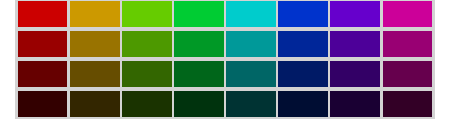
\includegraphics[keepaspectratio]{04_symbolizing_features_files/figure-pdf/fig-lightness-1.pdf}}

}

\caption{\label{fig-lightness}Eight different hues (across columns) with
decreasing lightness values (across rows).}

\end{figure}%

\subsection{Saturation}\label{saturation}

\textbf{Saturation}--also referred to as chroma--describes the intensity
or vividness of a color. Highly saturated colors appear bold and
vibrant, while low-saturation colors appear muted or grayish. In
cartographic design, saturation can be used to \textbf{emphasize
specific features} or categories, but it should be applied with care.
Overuse can lead to visual clutter or misinterpretation, especially when
combined with other color dimensions. Saturation is best used to subtly
enhance contrast or draw attention to key map elements.

\begin{figure}[H]

\centering{

\pandocbounded{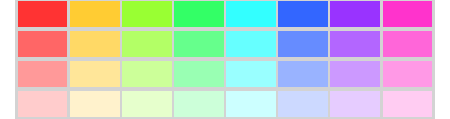
\includegraphics[keepaspectratio]{04_symbolizing_features_files/figure-pdf/fig-saturation-1.pdf}}

}

\caption{\label{fig-saturation}Eight different hues (across columns)
with decreasing saturation values (across rows).}

\end{figure}%

\section{Color Space}\label{color-space}

The three perceptual dimensions of color--hue, lightness, and
saturation--can be visualized as forming a \textbf{three-dimensional
color space}. While one might expect this space to be a \textbf{cube},
it is more accurately represented as a \textbf{cone}: hue wraps around
the circumference, saturation extends outward from the center, and
lightness runs vertically.

\begin{figure}[H]

\centering{


\includegraphics[width=1.28in,height=\textheight,keepaspectratio]{img/Color_space_std_small.jpg}

}

\caption{\label{fig-color_space}A conventional hue-saturation-lightness
color space. Hue varies around the circumference, saturation increases
outward from the center, and lightness varies vertically.}

\end{figure}%

This model helps explain how colors blend, fade, or become
indistinguishable as saturation or lightness changes.

However, most software-defined color spaces assume symmetry which does
not reflect how humans actually perceive color. For example, we can
distinguish more shades of blue than yellow at the same saturation and
lightness.

\begin{figure}[H]

\centering{

\pandocbounded{
\includegraphics[keepaspectratio]{04_symbolizing_features_files/figure-pdf/fig-munsell-1.pdf}}

}

\caption{\label{fig-munsell}A cross section of the color space with
constant hues and lightness values and decreasing saturation values
where the two hues merge.}

\end{figure}%

How many distinct yellows can you perceive? How many distinct blues? Do
the counts seem to match? Unless you have exceptionally acute color
vision, you'll likely notice a discrepancy--even though the software has
generated exactly 30 distinct shades of each. To confirm this, we can
add borders around each color swatch to visually verify that the number
of distinct colors is indeed the same.

\begin{figure}[H]

\centering{

\pandocbounded{
\includegraphics[keepaspectratio]{04_symbolizing_features_files/figure-pdf/fig-munsell_bis-1.pdf}}

}

\caption{\label{fig-munsell_bis}A cross section of the color space with
each color distinctly outlined.}

\end{figure}%

By now, it should be evident that symmetrical color spaces---like those
commonly used in software--do not accurately reflect how humans perceive
color. Our visual system is more sensitive to certain hues and less so
to others, resulting in perceptual asymmetries that these models fail to
capture. More rigorously designed color spaces, such as \textbf{CIELAB}
and \textbf{Munsell}, address this limitation by modeling color as a
non-symmetrical space that better aligns with human perception.

The Munsell color space is designed so that equal visual differences
correspond more closely to equal perceptual differences.

\begin{figure}[H]

\centering{

\pandocbounded{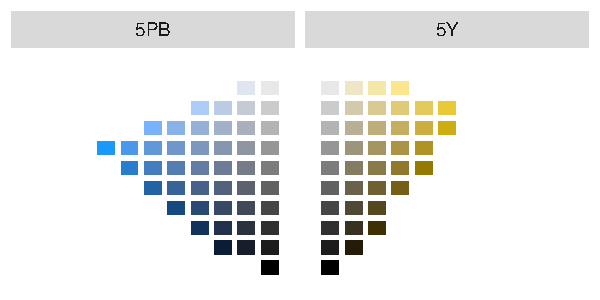
\includegraphics[keepaspectratio]{04_symbolizing_features_files/figure-pdf/fig-munsell_slice-1.pdf}}

}

\caption{\label{fig-munsell_slice}A slice of the Munsell color space
illustrating that the range of distinguishable colors varies by hue,
reflecting human color perception more accurately than symmetrical HSV
models.}

\end{figure}%

As illustrated by the Munsell color space, our ability to distinguish
colors is not uniform across hues. For example, we can perceive fewer
distinct shades of yellow than blue at comparable lightness levels. In
one comparison, 29 unique shades of yellow were discernible (excluding
grayscale values where saturation = 0), while 36 shades of blue were
distinguishable.

Understanding how humans perceive color helps us choose colors that
communicate data effectively. The next step is determining how colors
should be assigned to map features based on the type of data being
mapped.

The next section introduces three foundational color
schemes--\textbf{qualitative}, \textbf{sequential} and
\textbf{divergent}--each tailored to different types of data and mapping
goals.

\section{Color Schemes}\label{color-schemes}

Once you've selected an appropriate color space, the next step is to
determine how to apply color to your data. This involves choosing a
classification scheme--a method for grouping data values into discrete
\textbf{classes}, each of which is represented by a distinct
\textbf{color swatch}. The choice of classification scheme depends on
the nature of your data and the message you want your map to convey. In
the following sections, we'll explore three common color schemes:
\textbf{qualitative}, \textbf{sequential}, and \textbf{divergent}.

\subsection{Qualitative color scheme}\label{qualitative-color-scheme}

\textbf{Qualitative} color schemes are used to symbolize data that have
no inherent order--such as categories or types. These schemes assign
distinct hues to each class. To maintain perceptual balance, the hues
are typically chosen to have equal lightness and saturation, ensuring
that no category appears more prominent than another.

\begin{figure}[H]

\centering{

\pandocbounded{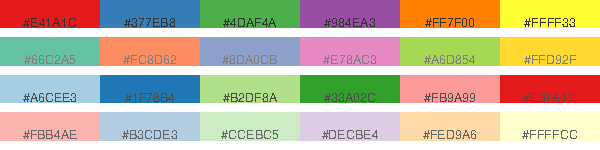
\includegraphics[keepaspectratio]{04_symbolizing_features_files/figure-pdf/fig-qualitative-1.pdf}}

}

\caption{\label{fig-qualitative}Example of four different qualitative
color schemes. Color hex numbers are superimposed on each palette.}

\end{figure}%

These schemes are ideal for mapping variables like land cover types,
political affiliations, or survey responses. However, care should be
taken when selecting hues, especially in contexts where cultural
associations may influence interpretation. For example, it may not make
sense to assign \emph{blue} to Republican regions or \emph{red} to
Democratic ones on a political map.

\begin{figure}[H]

\centering{

\pandocbounded{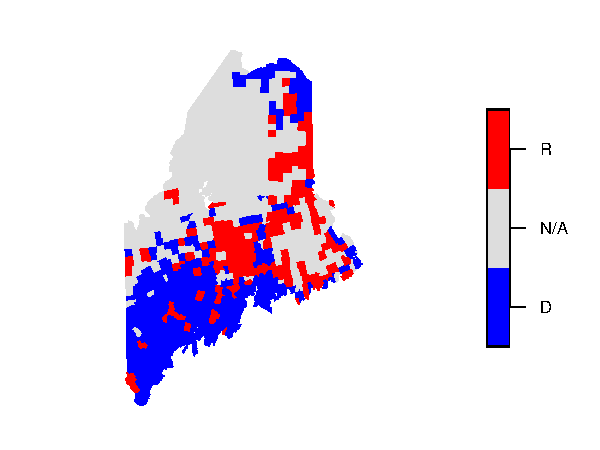
\includegraphics[keepaspectratio]{04_symbolizing_features_files/figure-pdf/fig-qualitative_map-1.pdf}}

}

\caption{\label{fig-qualitative_map}Map of 2012 election results shown
in a qualitative color scheme. Note the use of three hues (red, blue and
gray) of equal lightness and saturation.}

\end{figure}%

\subsection{Sequential color scheme}\label{sequential-color-scheme}

\textbf{Sequential} color schemes are used to represent data that follow
a meaningful order, such as income, temperature, elevation, or infection
rates. These schemes typically progress from light to dark, with lighter
shades representing lower values and darker shades representing higher
ones. This visual gradient helps convey magnitude and direction in the
data. Most sequential schemes use a single hue, but some may incorporate
two hues to emphasize a broader range of values.

\begin{figure}[H]

\centering{

\pandocbounded{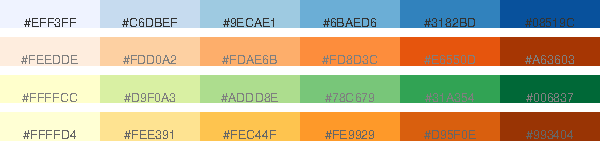
\includegraphics[keepaspectratio]{04_symbolizing_features_files/figure-pdf/fig-sequential-1.pdf}}

}

\caption{\label{fig-sequential}Example of four different sequential
color schemes. Color hex numbers are superimposed on each palette.}

\end{figure}%

A \textbf{choropleth} map is a thematic map in which polygons are
symbolized according to the value of an associated attribute. The
symbolization is typically achieved using colors grouped into discrete
classes or displayed as a continuous gradient. Choropleth maps are
widely used to visualize spatial variation in quantities such as income,
population density, housing value, and unemployment rates. Because the
appearance of a choropleth map depends on both the choice of color
scheme and the method used to classify the data, different
representations of the same dataset can emphasize different spatial
patterns.

The following example shows a \textbf{choropleth} map of household
income in Maine using a green sequential color scheme.

\begin{figure}[H]

\centering{

\pandocbounded{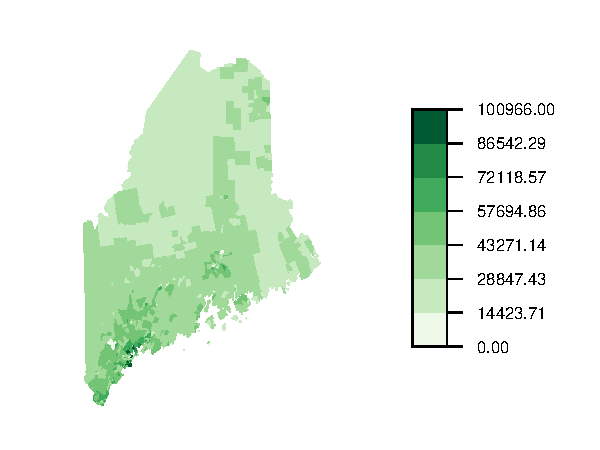
\includegraphics[keepaspectratio]{04_symbolizing_features_files/figure-pdf/fig-sequential_MAP-1.pdf}}

}

\caption{\label{fig-sequential_MAP}Map of household income (in dollars)
shown in a sequential color scheme. Note the use of a single hue (green)
and 7 different lightness levels.}

\end{figure}%

\subsection{Divergent color scheme}\label{divergent-color-scheme}

\textbf{Divergent} color schemes are used to represent ordered data that
revolve around a meaningful \textbf{central value}--such as a median,
mean, or zero. A divergent scheme is essentially two sequential schemes
joined at a common midpoint. These schemes are particularly effective
when the goal is to highlight differences on either side of a reference
point, making them well-suited for visualizing change, deviation, or
polarity.

A typical divergent scheme uses two contrasting hues---one for values
below the center and one for values above. Lightness and saturation are
adjusted symmetrically to reflect the magnitude of deviation from the
central value. This approach helps viewers quickly identify extremes and
interpret the direction and intensity of variation.

The following examples showcase several divergent palettes:

\begin{figure}[H]

\centering{

\pandocbounded{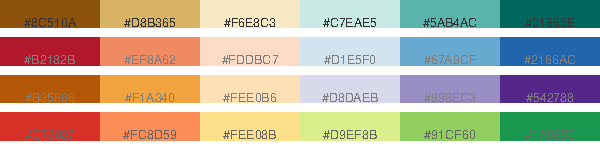
\includegraphics[keepaspectratio]{04_symbolizing_features_files/figure-pdf/fig-divergent-1.pdf}}

}

\caption{\label{fig-divergent}Example of four different divergent color
schemes. Color hex numbers are superimposed onto each palette.}

\end{figure}%

Building on the income data from the previous section, we can also
represent income using a divergent color scheme--particularly useful
when emphasizing variation around a central value. In this case, we
center the scheme on the median household income of \$36,641. Values
below the median are shown using a brown hue, while values above the
median are represented with a green-blue hue. Each hue is further
divided into progressively lighter or darker shades to reflect the
degree of deviation from the median, allowing for a more nuanced
interpretation of income disparities across regions.

\begin{figure}[H]

\centering{

\pandocbounded{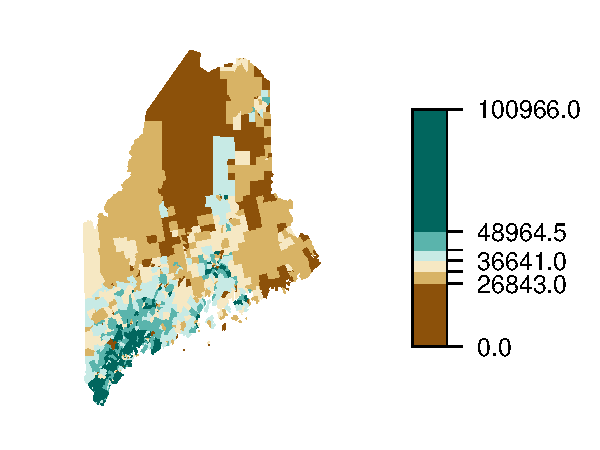
\includegraphics[keepaspectratio]{04_symbolizing_features_files/figure-pdf/fig-divergent_map-1.pdf}}

}

\caption{\label{fig-divergent_map}This map of household income uses a
divergent color scheme where two different hues (brown and blue-green)
are used for two sets of values separated by the median income of
\$36,641. Each hue is further divided into progressively lighter or
darker shades.}

\end{figure}%

\section{Choosing an Appropriate Color
Scheme}\label{choosing-an-appropriate-color-scheme}

Selecting the right color scheme for your map depends on both the nature
of your data and the number of classes you wish to represent.
Fortunately, most modern GIS software packages, including ArcGIS Pro and
QGIS, provide built-in qualitative, sequential, and divergent color
schemes that have been designed to be perceptually balanced and
cartographically effective. As a result, users rarely need to create
color schemes from scratch.

Many of these palettes are derived from or inspired by
\textbf{\href{http://colorbrewer2.org/}{ColorBrewer}}, a widely used
resource developed by Cynthia Brewer and colleagues at Pennsylvania
State University. ColorBrewer offers curated palettes tailored to
different data types--qualitative, sequential, and divergent--and
provides guidance on selecting colorblind-safe schemes and palettes that
reproduce well in grayscale, making them especially useful for printed
maps.

\begin{figure}[H]

\centering{


\includegraphics[width=0.7\linewidth,height=\textheight,keepaspectratio]{img/ColorBrewer.png}

}

\caption{\label{fig-colorbrewer_site}The ColorBrewer website, which
provides cartographically designed qualitative, sequential, and
divergent color schemes.}

\end{figure}%

One important design consideration is the number of color swatches used.
ColorBrewer limits most schemes to 12 or fewer swatches, reflecting the
reality that human perception struggles to reliably distinguish more
than a handful of colors in a legend. For example, try matching nine
shades of green in a map to their corresponding legend entries--it
quickly becomes a challenge.

\section{Classification Intervals}\label{classification-intervals}

The way data values are grouped into intervals can significantly affect
how a map looks and how its patterns are interpreted. In the previous
examples, two different classification schemes were used: an
\textbf{equal interval} scheme for the sequential map and a
\textbf{quantile interval} scheme for the divergent map.

Classification intervals define how the full range of data is divided
into discrete classes, each represented by a color swatch. Different
schemes produce different visual outcomes, even when applied to the same
dataset. For instance, \textbf{equal interval} schemes divide the data
range into evenly spaced segments, which is useful for uniformly
distributed data. In contrast, \textbf{quantile schemes} ensure that
each class contains an equal number of features, which can help balance
visual representation across a map.

Other options include the \textbf{Jenks natural breaks} method which
uses an algorithm to identify clusters in the data, optimizing class
boundaries to reflect inherent groupings. The following figure compares
these three schemes--quantile, equal interval, and Jenks--applied to the
same income dataset. Notice how each scheme emphasizes different aspects
of the distribution.

\begin{figure}[H]

\centering{


\includegraphics[width=0.9\linewidth,height=\textheight,keepaspectratio]{img/Three_breaks_compared_2.png}

}

\caption{\label{fig-diff_class}The same income dataset classified using
quantile, equal interval, and Jenks natural breaks methods. Note how
different interval schemes reveal different spatial patterns.}

\end{figure}%

The \textbf{quantile interval} scheme ensures that each color swatch is
represented an equal number of times. If we have 20 polygons and 5
classes, the interval breaks will be such that each color is assigned to
4 different polygons.

The \textbf{equal interval} scheme divides the range of values into
equal interval widths. If the polygon values range from 10,000 to 25,000
and we have 5 classes, the intervals will be {[}10,000 ; 13,000{]},
{[}13,000 ; 16,000{]}, \ldots, {[}22,000 ; 25,000{]}.

The \textbf{Jenks interval} scheme (aka natural breaks) uses an
algorithm that identifies clusters in the dataset. The number of
clusters is defined by the desired number of intervals.

It may help to view the breaks when superimposed on top of a
distribution of the attribute data. In the following figure, the three
classification intervals are superimposed on a histogram of the
per-household income data. The histogram shows the distribution of
values as ``bins'' where each bin represents a range of income values.
The y-axis shows the frequency (or number of occurrences) for values in
each bin.

\begin{figure}[H]

\centering{


\includegraphics[width=0.9\linewidth,height=\textheight,keepaspectratio]{img/Three_hist_intervals.png}

}

\caption{\label{fig-diff_maps}Three different classification intervals
used in the three maps. Note how each interval scheme encompasses
different ranges of values.}

\end{figure}%

\section{Summary}\label{summary-2}

This chapter introduces key principles for symbolizing spatial data
using color and classification schemes to improve map readability and
interpretation.

\begin{itemize}
\tightlist
\item
  \textbf{Color Dimensions}: Explains how hue, lightness, and saturation
  represent different data types--categorical, ordered, and intensity
  based--and how they interact \textbf{perceptually}.
\item
  \textbf{Color Spaces}: Highlights the limitations of symmetrical
  hue-saturation-lightness models and introduces perceptually accurate
  alternatives such as \textbf{CIELAB} and \textbf{Munsell}.
\item
  \textbf{Color Schemes}: Describes three main approaches:

  \begin{itemize}
  \tightlist
  \item
    \textbf{Qualitative} for unordered categories,
  \item
    \textbf{Sequential} for ordered data,
  \item
    \textbf{Divergent} for data centered around a meaningful midpoint.
  \end{itemize}
\item
  Color Selection Tools: Introduces \textbf{ColorBrewer} for choosing
  effective, accessible palettes.
\item
  \textbf{Choropleth Maps}: Introduces choropleth maps as thematic maps
  in which polygons are symbolized according to attribute values and
  explains how qualitative, sequential, and divergent color schemes can
  be used to communicate different types of data.
\item
  \textbf{Classification Intervals}: Compares equal interval, quantile,
  and Jenks natural breaks, showing how each affects data
  representation.
\end{itemize}

\chapter{Statistical maps}\label{statistical-maps}

\section{Introduction}\label{introduction-4}

In the previous chapter, equal interval and quantile classification
schemes were introduced as tools for symbolizing choropleth maps. In
this chapter, we revisit these methods from a statistical perspective
and explore additional classification approaches that are based on the
underlying distribution of the data.

This chapter builds on those foundations by focusing on the statistical
principles that underlie map classification. A key challenge in
choropleth mapping is deciding how to convert a continuous distribution
of values into a manageable number of classes. Different classification
methods can produce very different representations of the same dataset
and may emphasize different spatial patterns. We therefore examine
several commonly used approaches, including equal intervals, quantiles,
boxplot-based classifications, and standard deviation units.

Even after selecting a classification scheme, an important question
remains: how much confidence should we place in the mapped patterns?
Many spatial datasets, particularly those derived from sample surveys,
are estimates accompanied by margins of error or standard errors. These
uncertainties can affect rankings, classifications, and the apparent
strength of spatial patterns. The chapter concludes by introducing
techniques for visualizing and evaluating uncertainty in statistical
maps.

By the end of this chapter, you should be able to select and interpret
common classification schemes and assess how uncertainty influences the
conclusions drawn from choropleth maps.

\section{Statistical distribution
maps}\label{statistical-distribution-maps}

Many spatial variables, such as income, temperature, elevation, or
population density, are measured on a continuous scale. As a result,
every geographic unit in a dataset can potentially have a unique value.
In a choropleth map, these values are represented by varying shades or
colors assigned to polygons. For example, a map of Massachusetts
displaying median household income could assign a unique color to every
census tract. Although this approach preserves the full variability in
the data, the resulting map can be visually overwhelming and may obscure
broader spatial patterns.

\begin{figure}[H]

\centering{

\pandocbounded{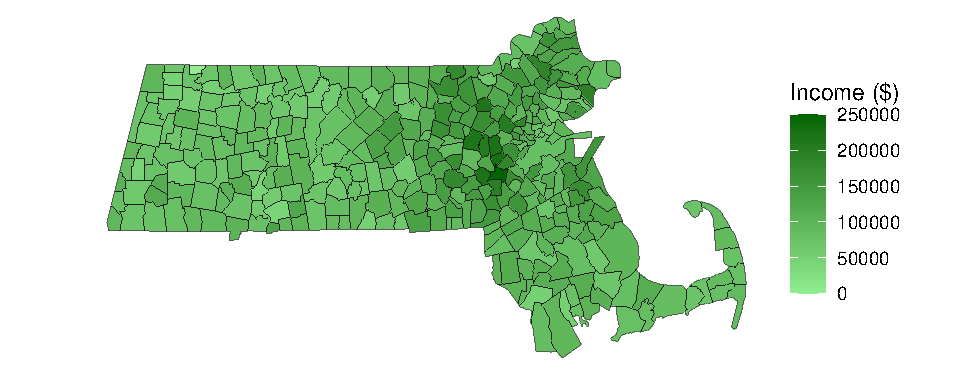
\includegraphics[keepaspectratio]{05_statistical_maps_files/figure-pdf/fig-continuous-1.pdf}}

}

\caption{\label{fig-continuous}Choropleth map of household income using
a continuous color gradient. Although each tract receives a color that
closely reflects its value, the large number of unique colors makes
broader spatial patterns difficult to identify.}

\end{figure}%

While technically accurate, such maps often obscure broader patterns and
make interpretation difficult. To improve interpretability, continuous
values are often grouped into a smaller number of classes before colors
are assigned to the map. The challenge then becomes determining where
the class boundaries should be placed.

\begin{figure}[H]

\centering{

\pandocbounded{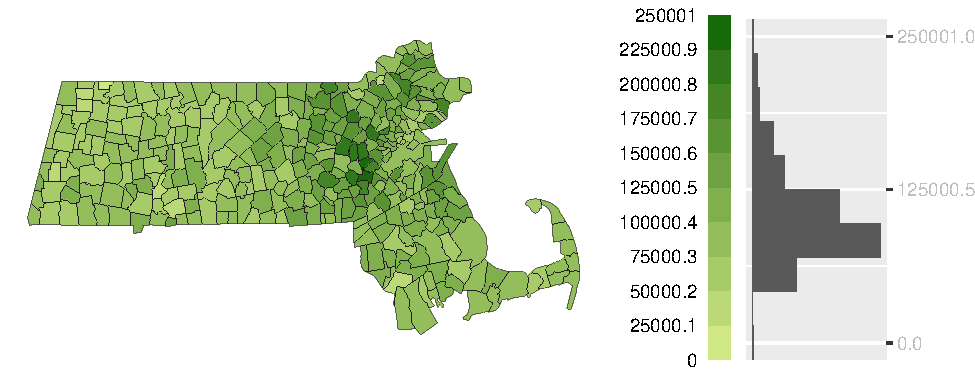
\includegraphics[keepaspectratio]{05_statistical_maps_files/figure-pdf/fig-equalint-1.pdf}}

}

\caption{\label{fig-equalint}Equal interval classification of household
income. The full range of income values is divided into 10 intervals of
equal width. The histogram shows the number of polygons assigned to each
interval, illustrating that equal-width classes do not necessarily
contain equal numbers of observations.}

\end{figure}%

The histogram accompanying the map is rotated vertically so that each
bin aligns with its corresponding color swatch in the legend. The length
of each gray bar represents the number of polygons assigned to that
class, allowing us to see how observations are distributed across the
classification intervals.

In an \textbf{equal interval} classification, the full range of values
is divided into intervals of equal width. As a result, each color swatch
represents the same span of income values, but not necessarily the same
number of polygons. This distinction is evident in the histogram, where
some classes contain many observations while others contain relatively
few. Because equal interval classification does not emphasize a central
reference point, a sequential color scheme--typically progressing from
light to dark--is used to represent increasing values.

\subsection{Quantile map}\label{quantile-map}

While an equal interval classification ensures that each color swatch
represents the same range of values, it does not guarantee that each
class contains the same number of polygons. When the data distribution
is skewed, some classes may contain many observations while others
contain only a handful.

\textbf{Quantile} classification takes the opposite approach by dividing
the data so that each class contains approximately the same number of
polygons. As a result, every color swatch appears with roughly equal
frequency on the map, often making spatial patterns and clusters easier
to identify.

\begin{figure}[H]

\centering{

\pandocbounded{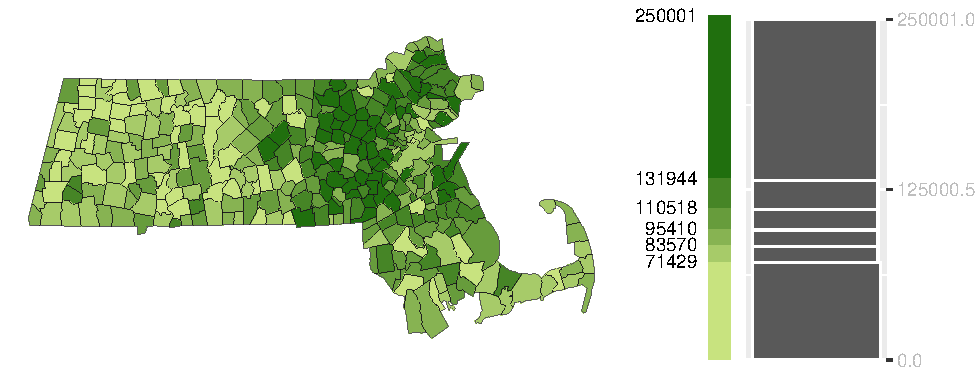
\includegraphics[keepaspectratio]{05_statistical_maps_files/figure-pdf/fig-quantile-1.pdf}}

}

\caption{\label{fig-quantile}Quantile classification of household
income. Each class contains approximately the same number of polygons,
although the range of income values represented by each class may differ
substantially.}

\end{figure}%

Unlike the equal interval choropleth map, the class widths shown in the
legend are not equal. Some color swatches represent a narrow range of
income values while others represent a much wider range. This occurs
because the classification is designed to place approximately the same
number of polygons into each class. The histogram illustrates this
tradeoff: the bars are more balanced in height than in the equal
interval example, but the intervals themselves vary considerably in
width.

Quantile choropleth maps are particularly useful for exploratory
analysis because they emphasize relative rankings and ensure that all
classes are well represented. However, this comes at a cost: the
intervals are not equal in width, and observations with very similar
values may be assigned to different classes while observations with very
different values may be placed in the same class.

Equal interval and quantile maps represent two common approaches to
classification: one prioritizes equal value ranges, while the other
prioritizes equal numbers of observations. The next methods use summary
statistics from the distribution itself to define class boundaries.

\subsection{Boxplot map}\label{boxplot-map}

Equal interval and quantile classifications divide the distribution into
classes using either the range of values or the number of observations.
A \textbf{boxplot} classification takes a different approach by using
\textbf{summary statistics} derived directly from the distribution
itself. A boxplot summarizes a distribution using measures of location
and spread, including the lower quartile (Q1), median, upper quartile
(Q3), and whiskers that extend toward the most extreme non-outlying
observations. It also identifies observations that fall unusually far
from the rest of the data, commonly referred to as outliers. The
distance between Q1 and Q3 is known as the interquartile range (IQR) and
contains the middle 50\% of the observations.

In the context of mapping, these summary statistics can be used to
define classification breaks. A \textbf{boxplot map} applies color
swatches to polygons based on where their values fall within the
boxplot-defined intervals.

This method is particularly useful when the goal is to highlight the
shape of the distribution--whether it is symmetrical, skewed, or
contains outliers. Because the boxplot includes a measure of centrality
(the median), a divergent color scheme is often appropriate. This allows
the map to visually emphasize deviations from the center, helping to
identify regions that are unusually high or low relative to the bulk of
the data.

Unlike the previous examples, the following graphic is a boxplot rather
than a histogram because the classification breaks are derived directly
from boxplot summary statistics.

\begin{figure}[H]

\centering{

\pandocbounded{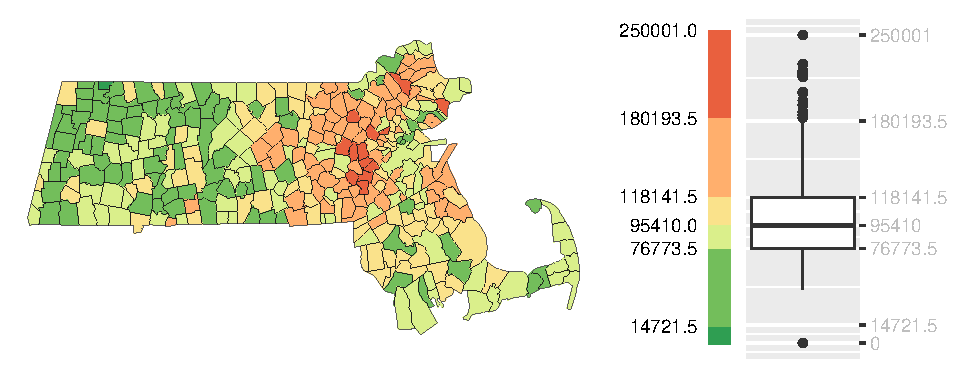
\includegraphics[keepaspectratio]{05_statistical_maps_files/figure-pdf/fig-boxmap-1.pdf}}

}

\caption{\label{fig-boxmap}Boxplot classification of household income.
Class boundaries are defined by the quartiles and whiskers of the income
distribution, creating categories that highlight the center, spread, and
potential outliers in the data.}

\end{figure}%

Boxplot choropleth maps are particularly useful when the objective is to
identify values that are typical, unusually high, or unusually low
relative to the rest of the distribution. Because the classification is
anchored to robust summary statistics rather than equal ranges or
counts, the resulting map is less sensitive to skewed distributions and
extreme values.

\subsection{IQR map}\label{iqr-map}

The boxplot map uses several summary statistics from the distribution to
create multiple classes. In some situations, however, our primary
interest is simply determining which observations fall within the
central portion of the distribution and which fall outside it. The
\textbf{interquartile range (IQR) map} simplifies the boxplot
classification by focusing on the middle 50\% of observations--those
lying between the first quartile (Q1) and third quartile (Q3). Values
are therefore grouped into three categories: below the IQR, within the
IQR, and above the IQR.

This approach is particularly useful when the goal is to highlight the
``core'' of the distribution--those observations that are neither
exceptionally high nor low. By emphasizing the middle range, the IQR map
can reveal spatial patterns that are less influenced by outliers or
extreme values. For example, while previous maps may have consistently
emphasized an east-west gradient in income across Massachusetts, the IQR
map may show that middle-income households are more evenly distributed
across the state.

Because the objective is to emphasize the middle of the distribution
rather than the extremes, the IQR category is often assigned the most
visually prominent color. In the following example, the middle 50\% of
income values are symbolized using a darker shade (black), while
observations above and below the IQR are shown using lighter shades.

\begin{figure}[H]

\centering{

\pandocbounded{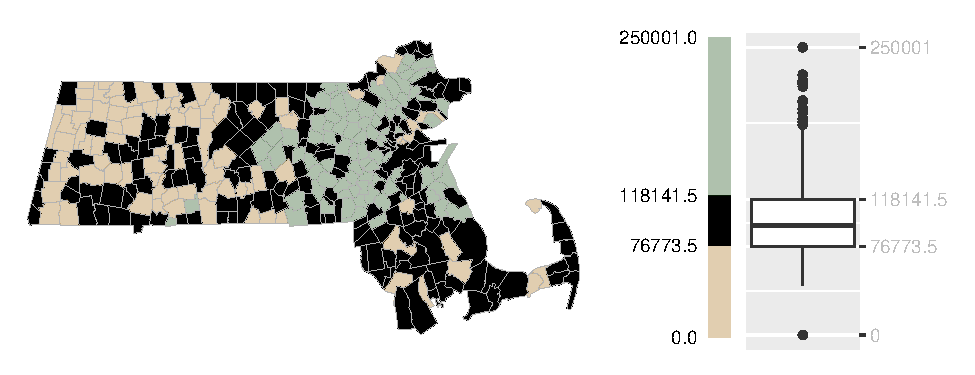
\includegraphics[keepaspectratio]{05_statistical_maps_files/figure-pdf/fig-iqr-1.pdf}}

}

\caption{\label{fig-iqr}IQR classification of household income. Black
polygons represent observations within the middle 50\% of the
distribution (between the first and third quartiles), while lighter
shades identify observations below and above this central range.}

\end{figure}%

Unlike previous classification schemes, the IQR map is not intended to
distinguish fine differences among all observations. Instead, it
emphasizes which regions are representative of the overall distribution
and which fall outside its central range.

\subsection{Standard deviation map}\label{standard-deviation-map}

Quantile maps and \textbf{standard deviation maps} both classify
observations according to their relationship to the overall
distribution. Quantile maps do so using percentiles, ensuring that each
class contains approximately the same number of observations. Standard
deviation maps take a different approach by measuring how far
observations fall above or below the mean. Rather than emphasizing an
observation's rank within the distribution, they emphasize its deviation
from the average.

When a dataset is approximately normally distributed (i.e., follows a
bell-shaped distribution), class boundaries can be defined using units
of standard deviation. A standard deviation map groups observations
according to their distance from the mean, with class breaks commonly
placed at ±1, ±2, and ±3 standard deviations.

Each class therefore represents a specific degree of departure from the
mean, making it easier to identify regions that fall within the expected
range and those that stand out as unusually high or low. For example,
observations within one standard deviation of the mean are often
considered typical, whereas those beyond two or three standard
deviations may be regarded as exceptional.

Standard deviation choropleth maps are particularly useful when the goal
is to evaluate how unusual a value is relative to the average rather
than to compare absolute ranges or percentile ranks. Because the
classification is centered on the mean, a divergent color scheme is
typically used, with a neutral color representing average values and
increasingly intense hues indicating greater departures above and below
the mean.

The accompanying histogram is overlaid with a normal distribution curve
because standard deviation classifications are most meaningful when the
underlying data are approximately bell-shaped. Unlike equal interval or
quantile maps, the class boundaries correspond to fixed distances from
the mean rather than equal value ranges or equal numbers of
observations.

\begin{figure}[H]

\centering{

\pandocbounded{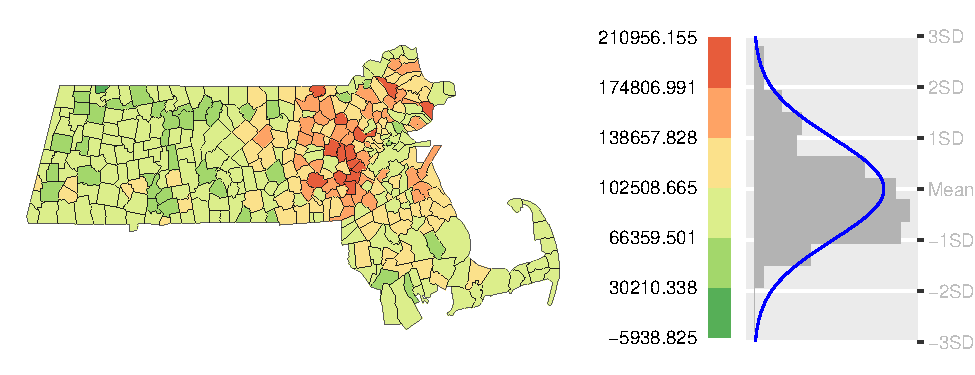
\includegraphics[keepaspectratio]{05_statistical_maps_files/figure-pdf/fig-sdmap-1.pdf}}

}

\caption{\label{fig-sdmap}Standard deviation classification of household
income. Class boundaries are defined by ±1, ±2, and ±3 standard
deviations from the mean income, allowing regions to be interpreted
according to their distance from the average.}

\end{figure}%

Standard deviation maps are most informative when the data are
approximately symmetrical and the mean provides a meaningful measure of
central tendency. For highly skewed distributions or datasets containing
extreme outliers, the resulting classes may be unbalanced and can lead
to misleading interpretations. As with any classification method, the
suitability of a standard deviation map should be evaluated in the
context of the underlying distribution.

\subsection{Outlier maps}\label{outlier-maps}

The classification methods discussed thus far have focused on describing
the overall distribution of values by assigning every observation to a
meaningful class. In some situations, however, our primary interest is
not in the full distribution but in identifying the relatively small
number of observations that differ markedly from the rest. Such
observations are commonly referred to as outliers.

Outlier maps are designed to emphasize these unusually high or low
values while treating the remaining observations as a background
reference. They are particularly useful when the goal is to identify
regions that warrant further investigation, such as areas with
exceptionally high income, unusually low population density, or elevated
disease rates.

Importantly, there is no single definition of an outlier. Different
statistical approaches identify unusual observations in different ways,
often leading to different sets of highlighted regions. The following
sections introduce three common approaches: \textbf{boxplot outlier
map}, \textbf{standard deviation outlier maps} and \textbf{quantile
outlier maps}.

\subsubsection{Boxplot outlier map}\label{boxplot-outlier-map}

Recall that a boxplot identifies outliers as observations lying beyond
the whiskers, which typically extend 1.5 times the interquartile range
(IQR) beyond the first and third quartiles. A \textbf{boxplot outlier
map} applies this definition spatially by highlighting only those
observations that fall outside the whisker boundaries. Values within the
whiskers are grouped into a single background class, allowing unusually
high and low observations to stand out clearly.

\begin{figure}[H]

\centering{

\pandocbounded{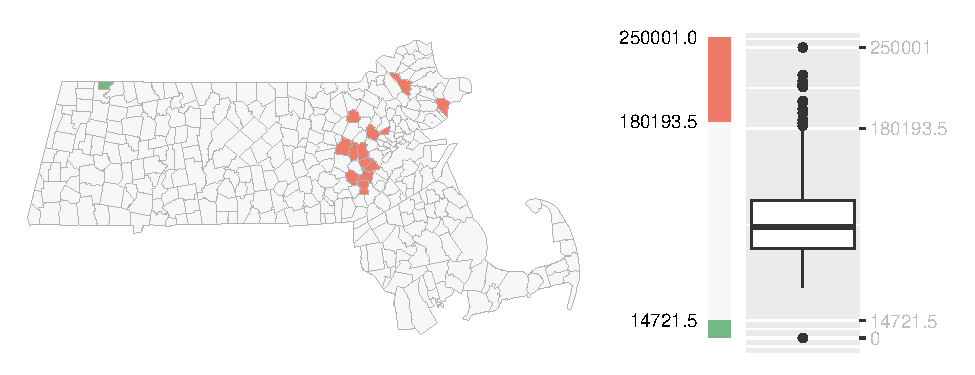
\includegraphics[keepaspectratio]{05_statistical_maps_files/figure-pdf/fig-outlier1-1.pdf}}

}

\caption{\label{fig-outlier1}Boxplot outlier map of household income.
Tracts with income values beyond the upper or lower boxplot whiskers are
highlighted, while all remaining tracts are grouped into a neutral
background class.}

\end{figure}%

You'll note the asymmetrical distribution of outliers, with more than a
dozen tracts identified as unusually high-income and only one tract
identified as unusually low-income. This imbalance reflects the
right-skewed nature of the income distribution, where a small number of
very high values extend farther from the bulk of the data than the
lowest values.

\subsubsection{Standard deviation outlier
map}\label{standard-deviation-outlier-map}

While a standard deviation map assigns all observations to classes based
on their distance from the mean, a \textbf{standard deviation outlier
map} focuses only on the most extreme departures from the average. A
common approach is to define outliers as observations that fall more
than two standard deviations above or below the mean. If the data are
approximately normally distributed, these thresholds correspond to the
outer tails of the distribution representing only a small fraction of
the observations. Values within ±2 standard deviations of the mean are
grouped into a neutral background category allowing unusually high and
low values to stand out more clearly.

\begin{figure}[H]

\centering{

\pandocbounded{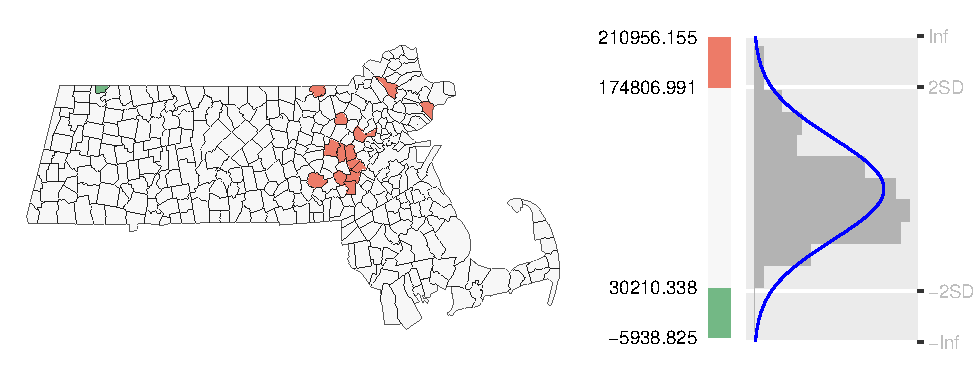
\includegraphics[keepaspectratio]{05_statistical_maps_files/figure-pdf/fig-outlier2-1.pdf}}

}

\caption{\label{fig-outlier2}Standard deviation outlier map of household
income. Regions with values beyond ±2 standard deviations from the mean
are highlighted, while all other regions are grouped into a neutral
background class.}

\end{figure}%

Unlike the boxplot outlier map, the observations identified here depend
directly on the mean and standard deviation of the dataset. As a result,
the regions highlighted as outliers may differ from those identified
using the boxplot approach, particularly when the distribution is skewed
or contains extreme values.

Because this method depends on the mean and standard deviation, it
performs best when the distribution is approximately symmetrical.

\subsubsection{Quantile outlier map}\label{quantile-outlier-map}

Unlike boxplot and standard deviation outlier maps, which define
outliers using specific statistical properties of the distribution, a
\textbf{quantile outlier map} defines outliers according to rank.
Observations are classified by their percentile position within the
dataset, and only those falling beyond selected percentile thresholds
are highlighted. For example, the upper and lower 2.5 percent of
observations can be identified by dividing the dataset into 40 quantiles
and mapping only the outermost classes.

Because quantile outlier maps are based on ranks rather than distances
from the mean or quartiles, they guarantee that a fixed proportion of
observations will be labeled as outliers. This makes them particularly
useful for skewed distributions where mean- or variance-based
definitions may perform poorly.

\begin{figure}[H]

\centering{

\pandocbounded{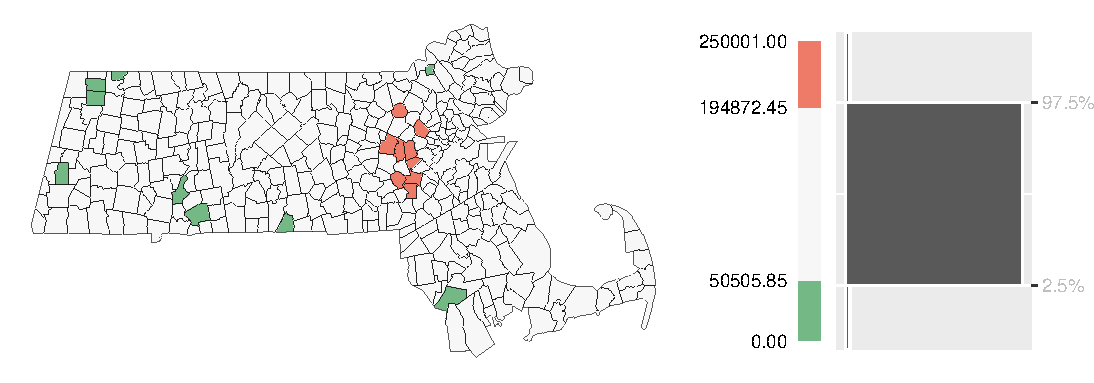
\includegraphics[keepaspectratio]{05_statistical_maps_files/figure-pdf/fig-outlier3-1.pdf}}

}

\caption{\label{fig-outlier3}Quantile outlier map of household income.
Regions falling within the lowest and highest 2.5 percent of values are
highlighted, while all remaining regions are grouped into a neutral
background category.}

\end{figure}%

Unlike the standard deviation outlier map, this approach identifies a
fixed proportion of observations as outliers regardless of the shape of
the distribution. As a result, some observations may be classified as
outliers even though they lie relatively close to the center of the
data. The method therefore emphasizes \textbf{relative rank} rather than
\textbf{statistical distance}.

Quantile outlier maps are particularly useful for exploratory analysis
because they provide a simple, distribution-free approach to identifying
unusually high and low observations. However, because the number of
outliers is determined by user-defined percentile thresholds, the
observations that are flagged are not necessarily statistically unusual.
Instead, they represent the highest- and lowest-ranked values in the
dataset.

The classification methods described so far assume that the mapped
values are known exactly. In practice, however, many spatial datasets
are estimates accompanied by uncertainty.

\section{Mapping uncertainty}\label{mapping-uncertainty}

Thus far, the classification methods presented in this chapter have
treated mapped values as if they were known exactly. In practice,
however, many spatial datasets---particularly those derived from sample
surveys such as the U.S. Census Bureau's American Community Survey
(ACS)---are estimates rather than direct measurements. As a result,
every estimate is accompanied by a measure of uncertainty.

Uncertainty is commonly expressed as either a \textbf{standard error
(SE)} or a \textbf{margin of error (MoE)}. These measures indicate how
much the reported estimate might vary from the true population value due
to sampling variability. For example, the ACS reports margins of error
based on a 90\% confidence interval, meaning that if many samples were
repeatedly drawn from the same population, approximately 90\% of the
resulting intervals would contain the true value.

This uncertainty presents an important challenge for map interpretation.
A map may suggest that one region has a higher income, population, or
unemployment rate than another, but if the uncertainty surrounding the
estimates is large, that apparent difference may not be statistically
meaningful. As a result, understanding uncertainty is often just as
important as understanding the estimates themselves.

One common approach to visualizing uncertainty is to create a separate
map showing the uncertainty measure alongside the map of estimated
values. The following figure presents an example using household income
estimates and their associated standard errors.

\begin{figure}[H]

\centering{

\pandocbounded{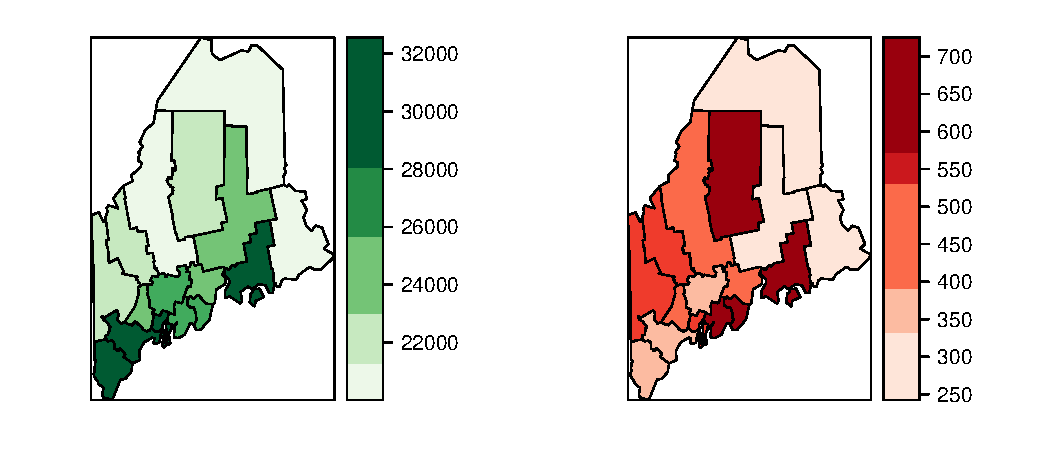
\includegraphics[keepaspectratio]{05_statistical_maps_files/figure-pdf/fig-map1-1.pdf}}

}

\caption{\label{fig-map1}Maps of household income estimates (left) and
their associated standard errors (right). Areas with high estimated
incomes do not necessarily have low uncertainty, highlighting the
importance of considering both maps when interpreting spatial patterns.}

\end{figure}%

While side-by-side maps separate estimates from uncertainty, they
require viewers to compare two visualizations simultaneously and
mentally integrate the information. An alternative is to overlay
uncertainty directly onto the estimate map using textures or hatch
marks. For example, a map of income estimates might use shades of green
to represent income levels, with different hatch patterns indicating the
degree of uncertainty. This approach allows viewers to assess both value
and reliability within a single display.

\begin{figure}[H]

\centering{


\includegraphics[width=0.7\linewidth,height=\textheight,keepaspectratio]{img/Income_and_uncertainty.jpg}

}

\caption{\label{fig-map2}Household income estimates represented by color
intensity and associated uncertainty represented by hatch patterns. The
map allows viewers to evaluate both the magnitude of an estimate and the
confidence that can be placed in it.}

\end{figure}%

Although overlay techniques allow estimates and uncertainty to be
displayed simultaneously, they require viewers to interpret two visual
variables at once. Another approach is to map the upper and lower bounds
of the confidence interval as separate maps. These maps provide a direct
representation of the range of plausible values but still require
viewers to compare multiple maps and mentally synthesize the
information.

\begin{figure}[H]

\centering{

\pandocbounded{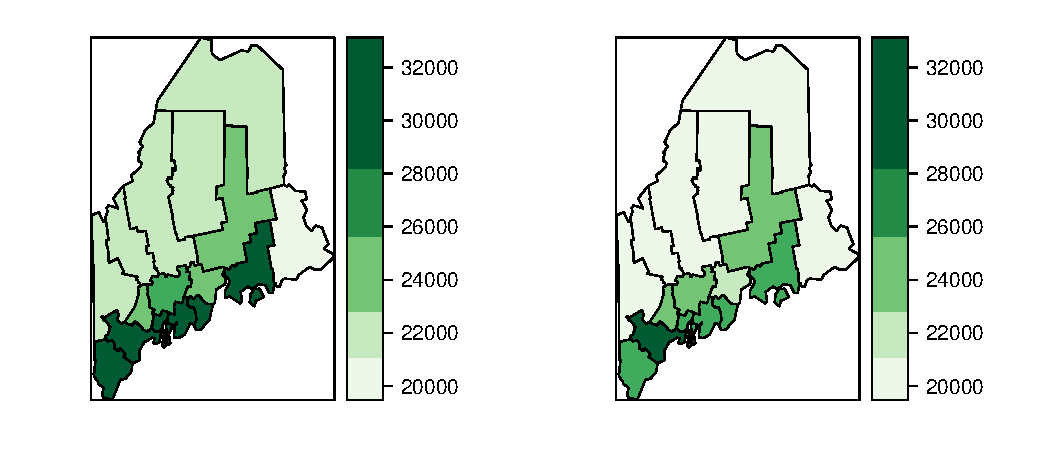
\includegraphics[keepaspectratio]{05_statistical_maps_files/figure-pdf/fig-map_MoE-1.pdf}}

}

\caption{\label{fig-map_MoE}Upper (left) and lower (right) bounds of the
90\% confidence interval for household income. Together, the maps depict
the range of plausible income values for each region.}

\end{figure}%

Mapping the upper and lower confidence limits provides a more complete
picture of uncertainty than a map of standard errors alone. By showing
the range of plausible values for each region, these maps help convey
the extent to which estimates may vary due to sampling error. However,
they still leave an important question unanswered: how does uncertainty
affect our interpretation of spatial patterns? Addressing this question
requires examining how rankings and spatial relationships change when
uncertainty is taken into account.

\subsection{Evaluating Spatial Patterns Under
Uncertainty}\label{evaluating-spatial-patterns-under-uncertainty}

While the maps presented earlier in this chapter offer ways to visualize
uncertainty such as margins of error or standard errors, they do not
fully address a key reason we map data in the first place: to compare
values across space. In spatial analysis, we are often interested in
identifying regions with relatively high or low values and ranking them
accordingly. These comparisons implicitly assume that the observed
estimates are stable and that their relative ordering would persist if a
different sample were collected. However, this assumption is not always
justified.

To explore this issue, we begin by examining confidence intervals
associated with each polygon's estimate. These intervals reveal that
many regions have overlapping ranges of plausible values, meaning that
the true value for one region could be higher or lower than that of a
neighboring region. For example, a county that appears to have a lower
income than another may, in fact, have a higher income once sampling
uncertainty is taken into account. Such overlap reduces our confidence
in spatial rankings and raises questions about the stability of the
patterns we observe on a map.

\begin{figure}[H]

\centering{

\pandocbounded{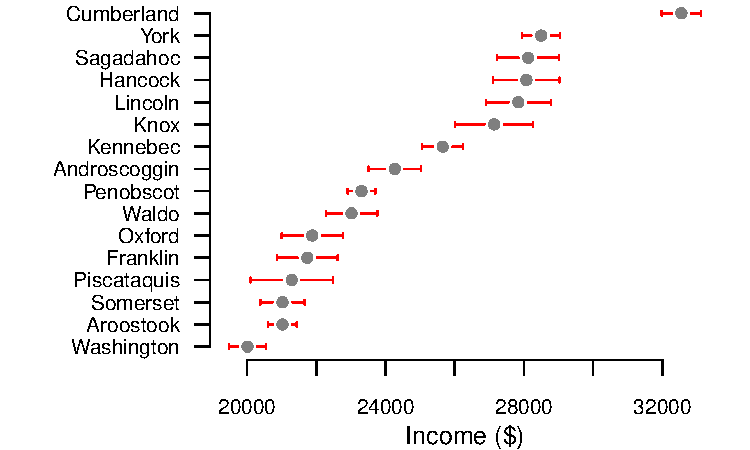
\includegraphics[keepaspectratio]{05_statistical_maps_files/figure-pdf/fig-MoE_plot1-1.pdf}}

}

\caption{\label{fig-MoE_plot1}County income estimates and their
associated 90\% confidence intervals. Note that many confidence
intervals overlap, indicating that apparent differences in county
rankings may not be statistically meaningful.}

\end{figure}%

Consider Piscataquis County, whose income estimate (represented by the
gray point in the plot) is lower than that of neighboring Oxford County.
Based solely on the point estimates, we might conclude that Oxford ranks
above Piscataquis in income. However, their 90\% confidence intervals
overlap substantially, indicating that this apparent difference may not
be statistically reliable. If a different sample were drawn from each
county, the resulting estimates could shift enough to reverse their
ranking. In other words, the ordering implied by the point estimates may
not reflect the ordering of the true underlying values. The following
example demonstrates how such rank reversals can occur when sampling
uncertainty is taken into account, potentially altering the spatial
patterns observed on a map.

\begin{figure}[H]

\centering{

\pandocbounded{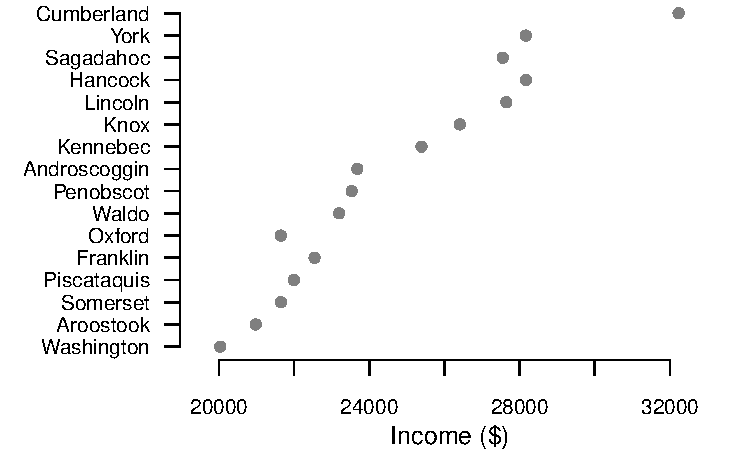
\includegraphics[keepaspectratio]{05_statistical_maps_files/figure-pdf/fig-sim_values-1.pdf}}

}

\caption{\label{fig-sim_values}One possible realization of county income
estimates generated from the 90\% confidence intervals. Note that the
ordering of several counties differs from that shown in the original
estimates.}

\end{figure}%

In one such simulated sample, Oxford County's income estimate falls
below those of both Piscataquis and Franklin counties, reversing their
original rankings. A similar shift occurs for Sagadahoc County, which
drops below Hancock and Lincoln counties. These changes illustrate how
sampling uncertainty can affect not only individual estimates but also
the relative ordering of regions. What appears to be a clear spatial
hierarchy in the original data may, in fact, be sensitive to the
particular sample used to generate the estimates.

But how do these shifts affect the geographic patterns we see on a map?
One way to assess this is to compare the \textbf{original} income map
with a \textbf{simulated} income map generated by randomly sampling
values within each county's confidence interval. Such a comparison
provides insight into the stability of observed spatial patterns and
helps reveal which features of the map are robust to uncertainty and
which may be artifacts of sampling variability.

\begin{figure}[H]

\centering{

\pandocbounded{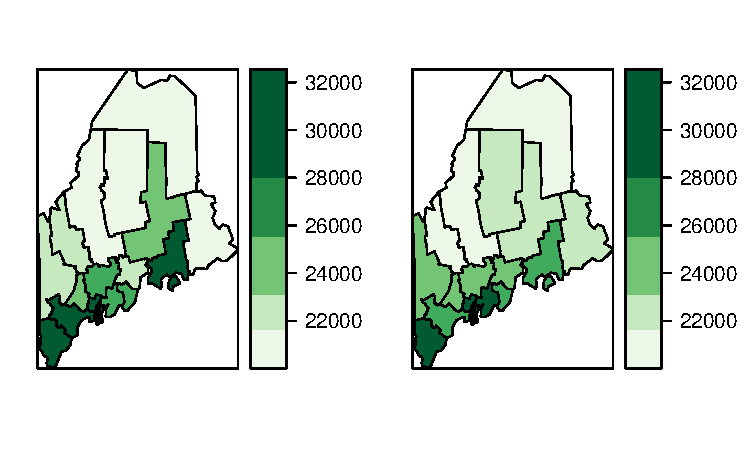
\includegraphics[keepaspectratio]{05_statistical_maps_files/figure-pdf/fig-sim_map-1.pdf}}

}

\caption{\label{fig-sim_map}Original county income estimates (left) and
one simulated realization generated from the associated 90\% confidence
intervals (right). Note that some counties change relative rank,
altering the spatial pattern of income across the state.}

\end{figure}%

The previous figure showed only one possible realization of the income
estimates. Because many values within each county's confidence interval
are plausible, numerous alternative maps could be generated. A few
additional simulated realizations are shown below.

\begin{figure}[H]

\centering{

\pandocbounded{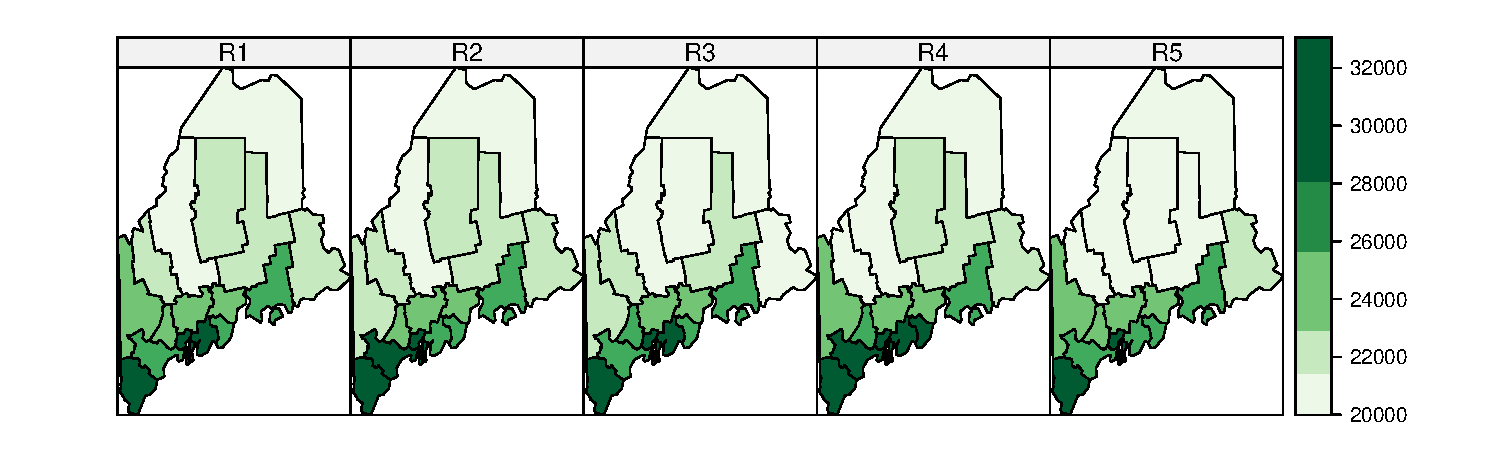
\includegraphics[keepaspectratio]{05_statistical_maps_files/figure-pdf/fig-sim_map2-1.pdf}}

}

\caption{\label{fig-sim_map2}Original county income estimates (left) and
four simulated maps generated from the associated 90\% confidence
intervals (R2--R5). Features that appear consistently across the
realizations are more likely to represent robust spatial patterns,
whereas features that vary among maps may be artifacts of sampling
variability.}

\end{figure}%

\subsection{Class comparison maps}\label{class-comparison-maps}

Effectively conveying both estimates and their associated uncertainty in
a single map remains a challenge. As Sun and Wong (Sun and Wong 2010)
note, the appropriate strategy often depends on the context and purpose
of the analysis. One useful approach is the \textbf{class comparison
method}, which evaluates whether a polygon's margin of error (MoE)
extends beyond the boundaries of its assigned classification. In a
choropleth map, class membership is often interpreted as meaningful
because polygons assigned to different classes are assumed to represent
different levels of the mapped variable. If uncertainty allows an
estimate to fall into one or more adjacent classes, confidence in that
classification is reduced. The class comparison method addresses this
issue by displaying not only the estimated value but also whether the
confidence interval surrounding that estimate crosses into neighboring
classes.

For example, if we adopt the classification breaks {[}0 , 20600 , 22800
, 25000 , 27000 , 34000 {]}, we find that many polygons have MoEs that
span multiple class boundaries.

\begin{figure}[H]

\centering{

\pandocbounded{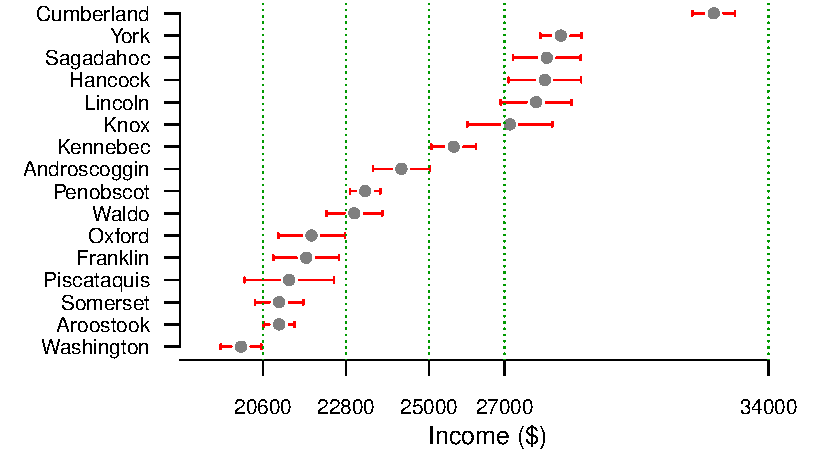
\includegraphics[keepaspectratio]{05_statistical_maps_files/figure-pdf/fig-compInt-1.pdf}}

}

\caption{\label{fig-compInt}County income estimates and their associated
90\% confidence intervals. Vertical dashed lines represent class
boundaries. Several confidence intervals cross into adjacent classes,
indicating uncertainty in class assignment.}

\end{figure}%

Consider Piscataquis County. Its income estimate falls within the second
classification interval (20600 to 22800 ), yet the lower end of its 90\%
confidence interval extends into the first interval. This means that we
cannot be 90\% confident that the county truly belongs in the second
class; its actual value may fall in the lower class instead. In
contrast, counties such as Cumberland and Penobscot have confidence
intervals that remain entirely within their assigned classes, providing
greater confidence in their classification.

Rather than requiring the reader to inspect confidence intervals
individually, this information can be incorporated directly into a
choropleth map using hatch patterns. The underlying color continues to
represent the estimated income value, while the hatch pattern indicates
whether the estimate's confidence interval extends beyond its assigned
class.

For example, income could be plotted using varying shades of green with
hatch symbols indicating if the lower interval crosses into a lower
class (135° hatch), if the upper interval crosses into an upper class
(45° hatch), if both interval ends cross into a different class
(90°-vertical-hatch) or if both interval ends remain inside the
estimate's class (no hatch).

\begin{figure}[H]

\centering{

\pandocbounded{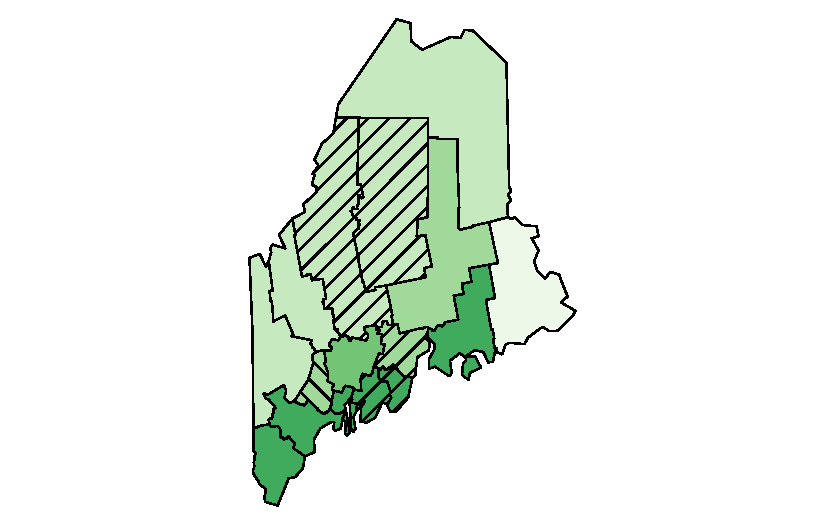
\includegraphics[keepaspectratio]{05_statistical_maps_files/figure-pdf/fig-ComPlot-1.pdf}}

}

\caption{\label{fig-ComPlot}Class comparison map of household income.
Colors represent income classes, while hatch patterns indicate whether
the associated confidence intervals remain within the assigned class or
extend into neighboring classes.}

\end{figure}%

Class comparison maps provide a practical way to visualize uncertainty
directly within a choropleth map. Rather than portraying uncertainty as
a separate variable, they focus on whether an observation's class
assignment is reliable. Regions with hatch marks should be interpreted
cautiously because their true values may belong to neighboring classes.
As a result, class comparison maps help distinguish robust
classifications from those that are sensitive to sampling variability.

\section{Summary}\label{summary-3}

This chapter explored statistical approaches to classifying and
interpreting continuous spatial data. Different classification methods
emphasize different aspects of a distribution and can produce very
different representations of the same dataset.

\begin{itemize}
\tightlist
\item
  \textbf{Equal interval maps} divide the range of values into classes
  of equal width and are useful when comparing absolute differences
  among observations.
\item
  \textbf{Quantile maps} assign approximately the same number of
  observations to each class, emphasizing relative rank and often
  revealing spatial patterns that may be hidden in equal interval maps.
\item
  \textbf{Boxplot, IQR, and standard deviation maps} use statistical
  properties of the distribution to define class boundaries and
  highlight different aspects of the data, such as central tendency,
  variability, and deviation from the mean.
\item
  \textbf{Outlier maps} focus attention on unusually high or low values
  using definitions based on boxplots, standard deviations, or
  quantiles.
\item
  The choice of classification scheme influences how spatial patterns
  are perceived and interpreted. No single method is universally
  superior; each has strengths and limitations that depend on the
  distribution of the data and the objectives of the analysis.
\item
  Many spatial datasets contain \textbf{uncertainty}, often expressed as
  a standard error or margin of error. Ignoring this uncertainty can
  lead to overconfidence in spatial rankings and apparent patterns.
\item
  \textbf{Confidence interval plots, simulated maps, and class
  comparison maps} provide ways to assess how uncertainty affects
  classifications, rankings, and the stability of observed spatial
  patterns.
\end{itemize}

Understanding both the statistical distribution of mapped values and the
uncertainty associated with those values leads to more informed and
defensible interpretations of choropleth maps.

\chapter{Pitfalls to avoid}\label{pitfalls-to-avoid}

\section{Introduction}\label{introduction-5}

While the previous chapter focused on uncertainty arising from sampling
error and estimation, this chapter examines sources of uncertainty and
bias that arise from how spatial data are represented, aggregated, and
interpreted.

Spatial data analysis offers powerful tools for uncovering patterns,
relationships, and insights across geographic space. However, with this
power comes a set of challenges that can easily mislead if not properly
understood and addressed. This chapter explores several common pitfalls
in spatial analysis, focusing on how data representation, aggregation,
and interpretation can distort our understanding of spatial phenomena.

We begin by examining how the representation of raw counts can create
misleading choropleth maps when differences in area or population are
ignored. We then explore how the choice of spatial units and aggregation
schemes can dramatically alter the appearance of spatial patterns, a
problem known as the \textbf{Modifiable Areal Unit Problem (MAUP)}.
Closely related to this issue is the \textbf{ecological fallacy}, where
inferences about individuals are mistakenly drawn from aggregate-level
data.

The chapter concludes by examining the challenges associated with
mapping rates, particularly when rates are based on small population
counts. These situations can produce unstable estimates that exaggerate
spatial variation and create misleading patterns. To address this
problem, we introduce techniques for normalizing data and smoothing
unstable rates.

\section{Representing Count}\label{representing-count}

Consider a 16km x 16km square study area populated by individuals
arranged in a perfect grid. The distribution is intentionally uniform so
that every location has the same underlying population density. If we
overlay two different zoning schemes--one using a regular grid and
another using irregular polygons--and count the number of individuals
within each zone, we produce two choropleth maps that suggest very
different spatial distributions. Yet, the underlying point pattern is
identical.

\begin{figure}[H]

\centering{

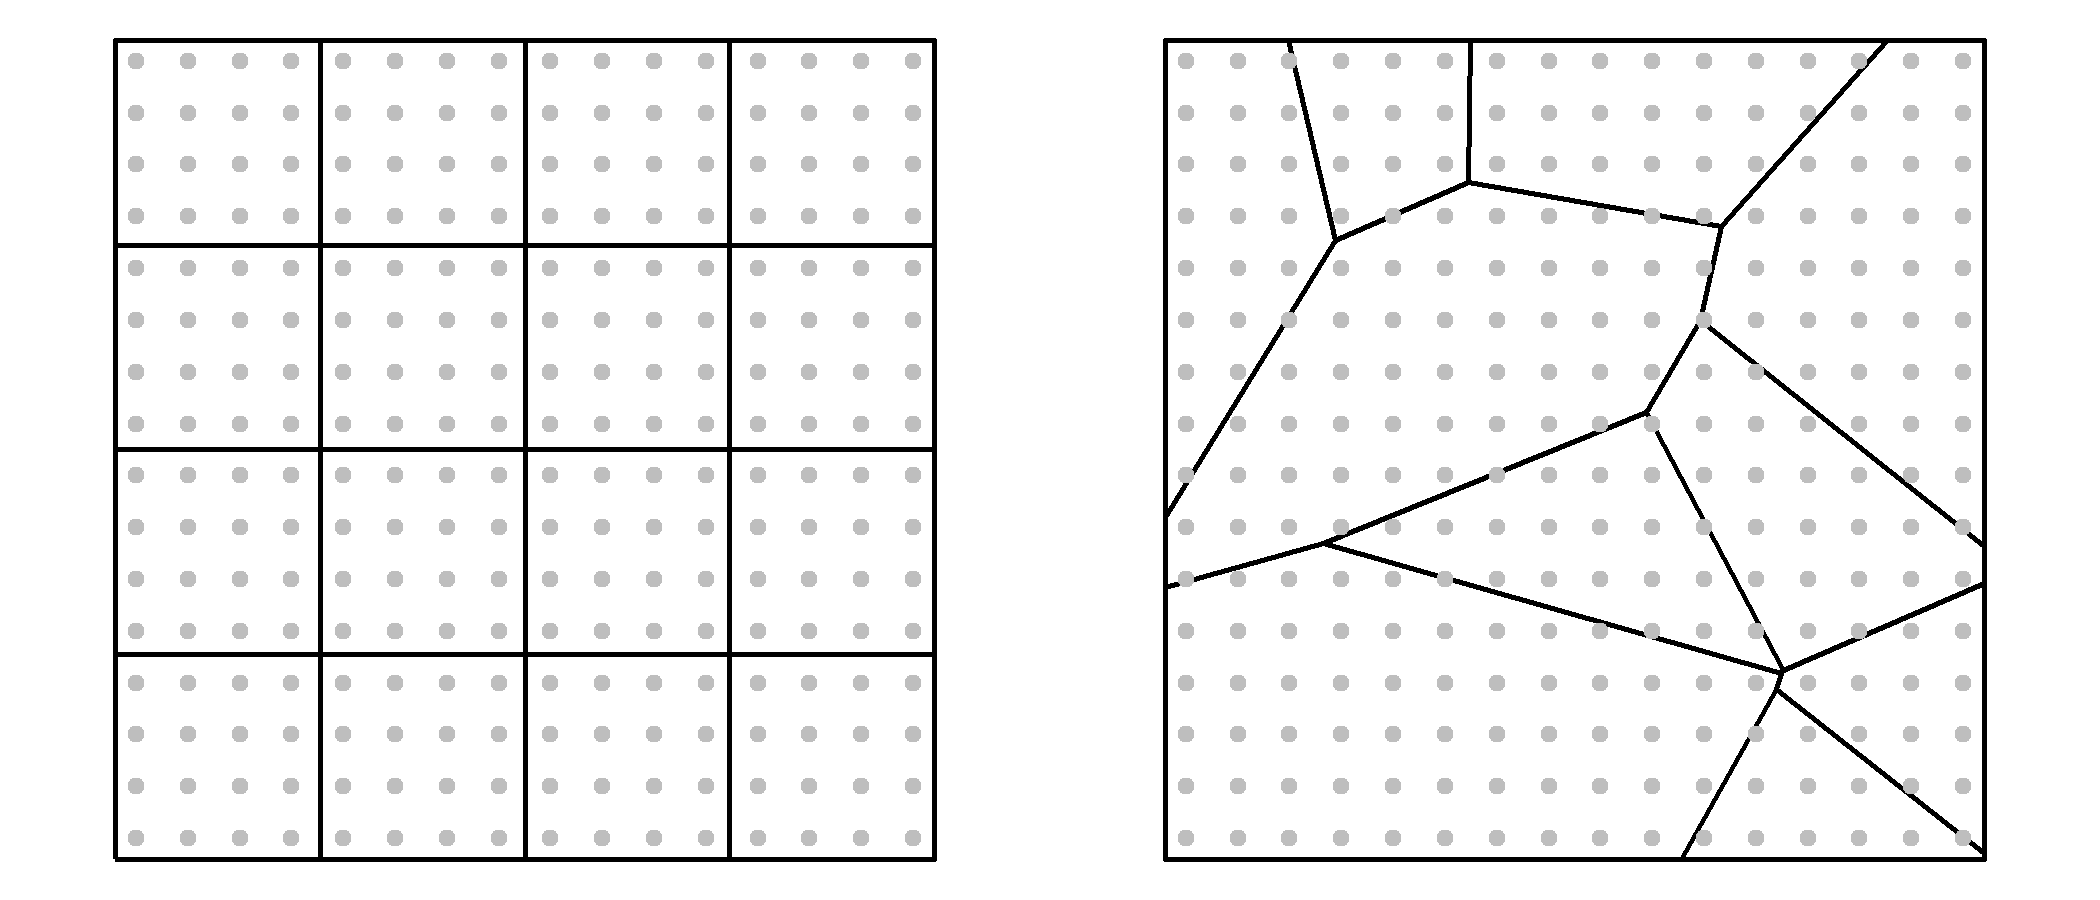
\includegraphics[width=5.20833in,height=\textheight,keepaspectratio]{img/grid_vs_tess_layout.png}

}

\caption{\label{fig-grid_vs_tess_layout}Uniformly distributed
individuals overlaid with two alternative zoning schemes: a regular grid
and an irregular tessellation. Although the underlying point pattern is
identical in both cases, the aggregation units differ.}

\end{figure}%

\begin{figure}[H]

\centering{

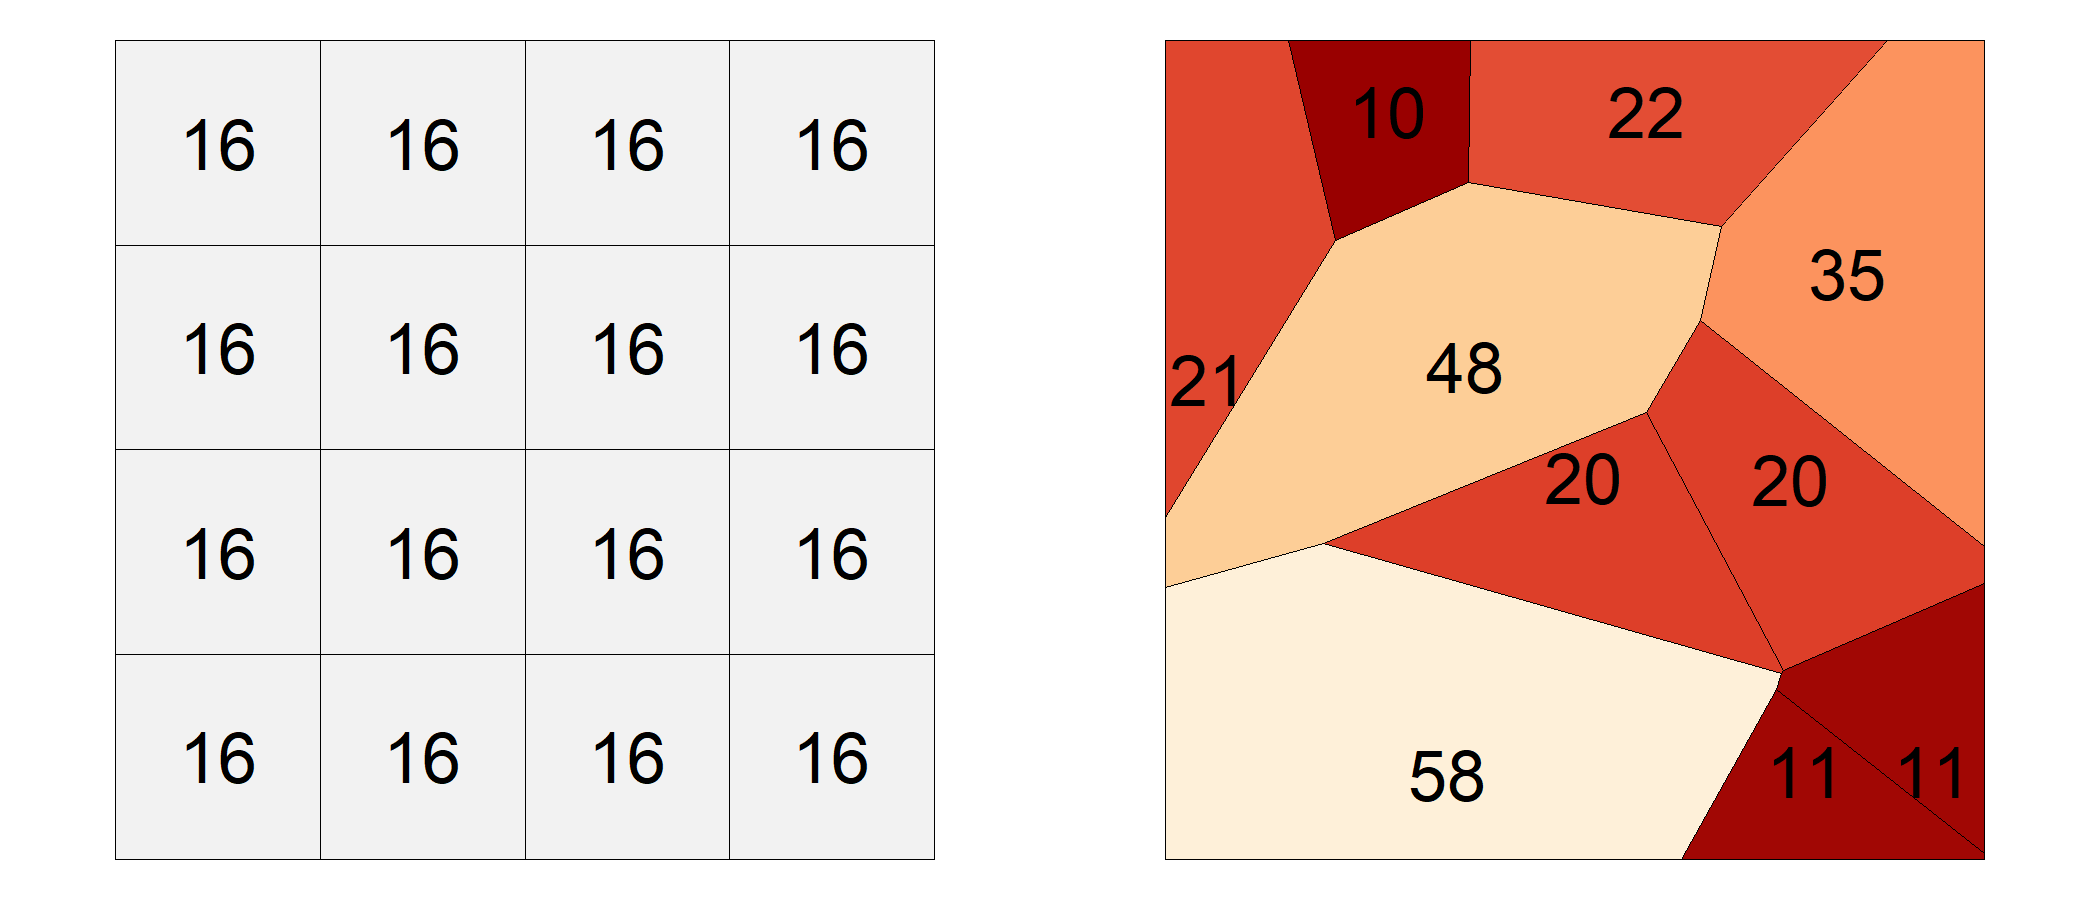
\includegraphics[width=5.20833in,height=\textheight,keepaspectratio]{img/grid_vs_tess_count.png}

}

\caption{\label{fig-grid_vs_tess_count}Raw counts summarized by two
different aggregation schemes. Although the underlying population
density is uniform, differences in polygon size and shape create the
appearance of different spatial patterns.}

\end{figure}%

This discrepancy illustrates a fundamental pitfall in spatial analysis:
counts are influenced not only by the phenomenon being measured but also
by the size and shape of the reporting units. Larger polygons tend to
accumulate larger counts than smaller polygons, even when the underlying
distribution is uniform. As a result, choropleth maps based on raw
counts can create misleading impressions of clustering or dispersion
where none exists.

To mitigate this issue, counts are often converted to ratios or rates.
For example, population can be expressed per square kilometer and
disease occurrence can be expressed per capita. These normalized
measures account for differences in polygon size or population and
therefore provide a more meaningful basis for comparison across regions.
In Figure~\ref{fig-grid_vs_tess_density}, switching from raw counts to
density maps reveals a more consistent and interpretable spatial
pattern.

\begin{figure}[H]

\centering{

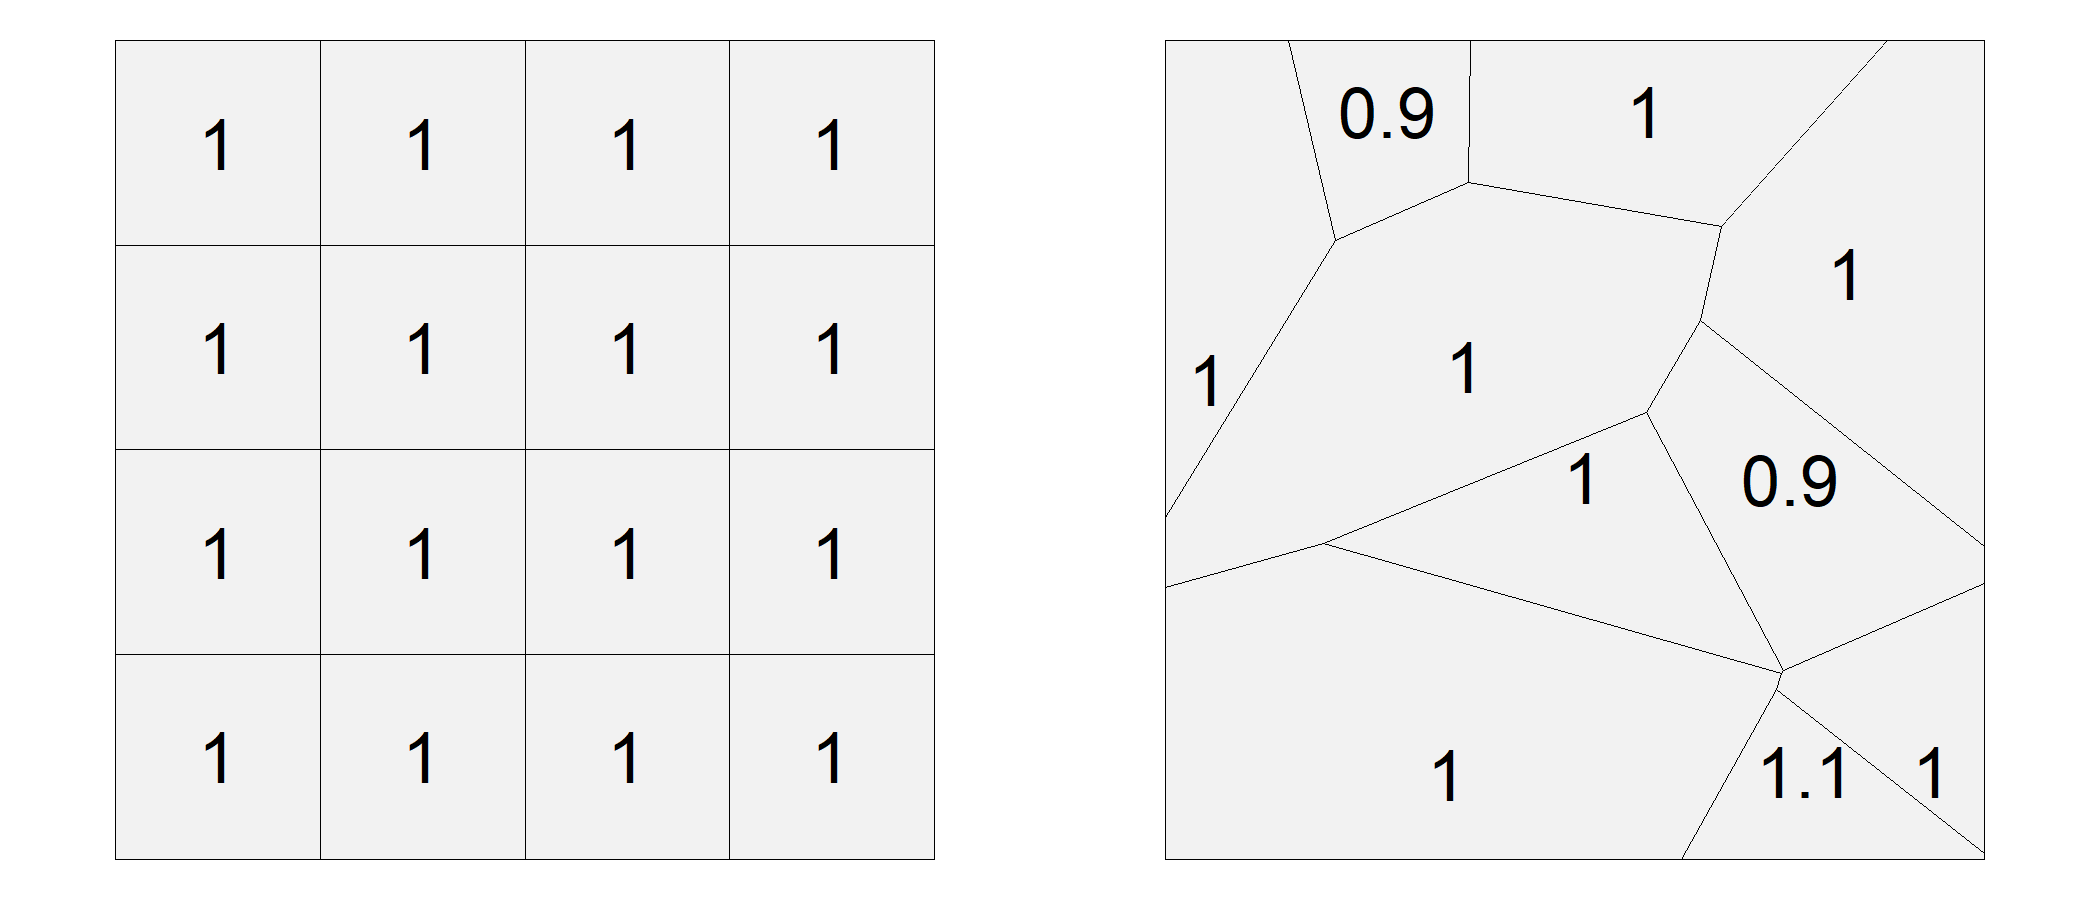
\includegraphics[width=5.20833in,height=\textheight,keepaspectratio]{img/grid_vs_tess_density.png}

}

\caption{\label{fig-grid_vs_tess_density}Point density choropleth maps
derived from the same underlying point pattern. Unlike the raw count
maps shown in Figure 6.2, the density maps reveal a nearly uniform
distribution regardless of the aggregation scheme. Minor deviations from
a density of 1 in the tessellated map occur because some polygon
boundaries do not coincide exactly with the spacing between points,
resulting in slight differences in the area assigned to each
observation.}

\end{figure}%

The same principle applies in many real-world applications. For example,
comparing disease counts across counties is often less informative than
comparing disease rates because counties differ dramatically in
population size.

\section{MAUP}\label{maup}

The \textbf{Modifiable Areal Unit Problem (MAUP)} (Openshaw 1983) is a
well-documented issue in spatial analysis that arises when data are
aggregated into spatial units such as census tracts, counties, or
states. These units are often arbitrary with respect to the phenomena
being studied. O'Sullivan and Unwin (O'Sullivan and Unwin 2010) further
emphasize that MAUP is not just a technical nuisance--it challenges the
validity of spatial inference when based on aggregated data.

Consider a uniform distribution of individuals across a study area, each
with two recorded variables: v1 and v2. The variables are symbolized as
varying shades of green and reds in the two left-hand maps of
Figure~\ref{fig-v1_and_v2_raw}.

\begin{figure}[H]

\centering{


\includegraphics[width=7.29167in,height=\textheight,keepaspectratio]{img/v1_and_v2_raw.png}

}

\caption{\label{fig-v1_and_v2_raw}Individual-level values for variables
v1 and v2. Although both variables exhibit spatial variation, there is
little or no relationship between them at the individual level, as
confirmed by the scatterplot.}

\end{figure}%

At the individual level, the relationship between v1 and v2 is
essentially absent. If aggregation preserved statistical relationships
perfectly, we would expect this lack of association to remain unchanged
after summarizing the data into larger spatial units. The following
examples demonstrate that this is not necessarily the case.

\begin{figure}[H]

\centering{

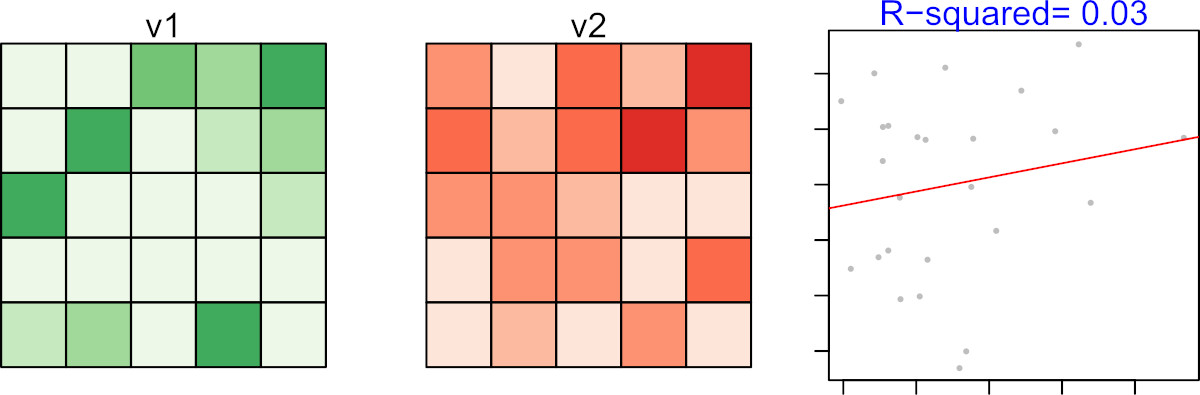
\includegraphics[width=6.77083in,height=\textheight,keepaspectratio]{img/unif_aggr.jpg}

}

\caption{\label{fig-v1_and_v2_unif}Data aggregated using a uniform
zoning scheme. Although the variables are uncorrelated at the individual
level, aggregation produces a weak positive relationship.}

\end{figure}%

If we then apply a non-uniform aggregation scheme, the correlation
appears even stronger, with a much higher \(R^2\) value.

\begin{figure}[H]

\centering{

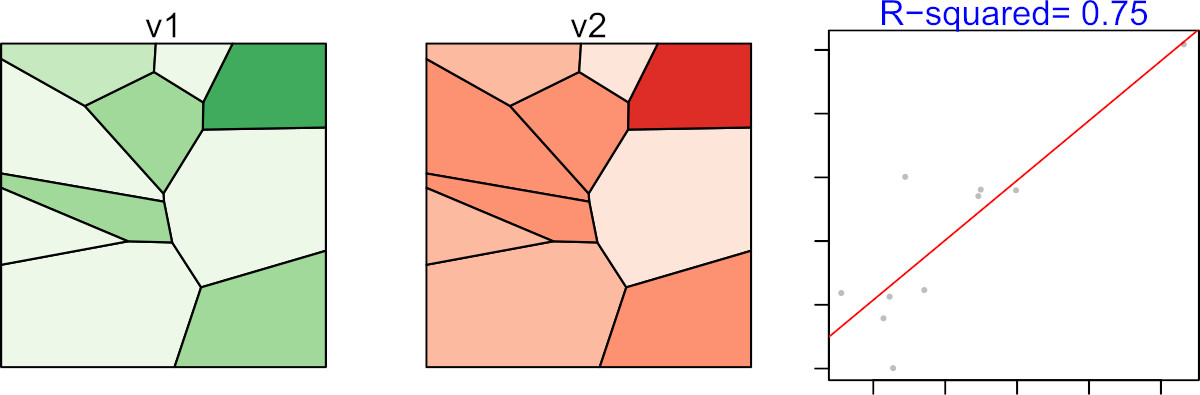
\includegraphics[width=6.77083in,height=\textheight,keepaspectratio]{img/irr_aggr.jpg}

}

\caption{\label{fig-v1_and_v2_nonunif}Data aggregated using a
non-uniform zoning scheme. The apparent relationship between v1 and v2
becomes substantially stronger despite the absence of such a
relationship at the individual level.}

\end{figure}%

This discrepancy is not due to any real relationship between v1 and v2,
but rather to the aggregation scheme itself. In fact, it is possible to
design an aggregation scheme that produces a near-perfect correlation
between two variables that are entirely uncorrelated at the individual
level. This is the essence of the Modifiable Areal Unit Problem:
analytical conclusions may depend as much on how the data are aggregated
as on the data themselves.

Because MAUP arises whenever aggregated data are analyzed, it also
creates an important interpretive challenge: relationships observed for
groups may not reflect relationships that exist for individuals. This
issue is explored in the next section as the ecological fallacy.

\section{Ecological Fallacy}\label{ecological-fallacy}

Whereas the MAUP concerns how aggregation can alter analytical results,
the ecological fallacy concerns how aggregated results are interpreted.
In practice, analysts are often constrained to working with data
summarized at the level of counties, census tracts, school districts, or
other reporting units. A common mistake is to assume that relationships
observed for these groups also apply to the individuals within them.
This error is known as the \textbf{ecological fallacy} (Freedman 1999).

For example, after observing the strong relationship in
Figure~\ref{fig-v1_and_v2_nonunif}, it might be tempting to conclude
that individuals with high values of v1 also tend to have high values of
v2. However, this conclusion does not follow from the data because the
relationship was observed \textbf{only after values were aggregated into
spatial units}. The observed correlation exists \emph{only} at the level
of the aggregated units--it may not hold, and often does not hold, at
the individual level.\\
To avoid the ecological fallacy, analysts should carefully distinguish
between the scale of the data and the scale of the conclusions being
drawn. It is appropriate to state, \emph{``At this level of aggregation,
we observe a strong relationship between v1 and v2,''}. but it is
incorrect to claim that this relationship necessarily exists at finer
scales. It is \emph{not} appropriate to conclude that the same
relationship necessarily exists among the individuals within those
aggregated units.

The ecological fallacy highlights the risks of interpreting aggregated
data. Another challenge arises when the aggregated values themselves are
unstable, particularly when they are expressed as rates based on small
populations. This issue is explored in the next section.

\section{Mapping rates}\label{mapping-rates}

You learned earlier in this chapter of the pitfalls in mapping raw
counts without accounting for differences in the size or shape of the
spatial units. In a rate calculation, the population at risk serves as
the denominator. When that denominator is small, the resulting rate can
become highly unstable.

To illustrate this, let's examine a series of maps showing kidney cancer
death rates by county for the period 1980-1984.

\begin{figure}[H]

\centering{


\includegraphics[width=5.72917in,height=\textheight,keepaspectratio]{img/raw_rates.png}

}

\caption{\label{fig-kidney0}Kidney cancer death rates by county for the
period 1980--1984. At first glance, the map suggests substantial
geographic variation in mortality risk.}

\end{figure}%

We begin by looking at the counties with the highest death rates:

\begin{figure}[H]

\centering{


\includegraphics[width=5.20833in,height=\textheight,keepaspectratio]{img/top10.png}

}

\caption{\label{fig-kidney1}Counties in the highest 10\% of kidney
cancer death rates. Surprisingly, many of these counties occur in
sparsely populated regions.}

\end{figure}%

Now compare this to the counties with the lowest death rates:

\begin{figure}[H]

\centering{


\includegraphics[width=5.20833in,height=\textheight,keepaspectratio]{img/bottom10.png}

}

\caption{\label{fig-kidney2}Counties in the lowest 10\% of kidney cancer
death rates. Note that many occur near counties with some of the highest
reported rates.}

\end{figure}%

At first glance, these maps suggest that both high and low rates are
clustered in similar regions. In fact, many of the counties with the
lowest rates are adjacent to those with the highest rates. This raises
questions: If environmental factors are driving kidney cancer mortality,
why would they affect one county but not its neighbor? Could differences
in local regulations or healthcare access explain the pattern?

Before jumping to conclusions, we need to examine the population counts
behind these rates:

\begin{figure}[H]

\centering{


\includegraphics[width=5.72917in,height=\textheight,keepaspectratio]{img/Population.png}

}

\caption{\label{fig-kidney3}Population count for each county. Note that
a quantile classification scheme is adopted forcing a large range of
values to be assigned a single color swatch.}

\end{figure}%

The central part of the states where we are observing both very high and
very low cancer death rates have low population counts. Recall that
population serves as the denominator used to compute the mortality rate.
Could population count have something to do with this odd congruence of
high and low cancer rates?

To explore this further, let's examine the relationship between death
rates and population counts:

\begin{figure}[H]

\centering{


\includegraphics[width=3.125in,height=\textheight,keepaspectratio]{img/Rate_vs_pop.png}

}

\caption{\label{fig-kidney_plot}Kidney cancer death rates versus county
population. Variability in the rates is much greater among counties with
small populations}

\end{figure}%

The scatterplot reveals a wide spread of rates among counties with small
populations. When we transform both axes to a logarithmic scale, the
pattern becomes clearer:

\begin{figure}[H]

\centering{


\includegraphics[width=3.125in,height=\textheight,keepaspectratio]{img/Rate_vs_pop_log.png}

}

\caption{\label{fig-kidney_plot_trans}Kidney cancer death rates versus
county population on logarithmic axes. The funnel-shaped pattern reveals
that rate variability decreases as population size increases.}

\end{figure}%

Here, we see that as population increases, the variability in death
rates decreases. This is expected: larger populations provide more
stable estimates of underlying rates. In contrast, small populations
produce unstable rates that can distort spatial patterns.

This issue is well-documented in spatial analysis literature. O'Sullivan
and Unwin (O'Sullivan and Unwin 2010) emphasize that mapping raw rates
without considering population size can lead to misleading
interpretations, especially in public health contexts.

To illustrate the problem, consider a county with a population of 1,000.
If the true death rate is 5 per 100,000, we would expect 0.05
deaths--that's less than one person. But if one person dies, the
observed rate in that county becomes 1 per 1,000, or 100 per
100,000--twenty times higher than the expected rate! This demonstrates
how \textbf{small denominators can inflate rates} and create artificial
hotspots and coldspots.

Rates computed from small denominator values are often referred to as
\textbf{unstable rates} because even small changes in the numerator can
produce large changes in the estimated rate. While this chapter uses
disease mortality rates as an example, the same problem can arise when
mapping the percentage of electric vehicles, unemployment rates, housing
vacancy rates, or any other measure based on a small underlying count.

The next section introduces one approach--Empirical Bayes smoothing--for
reducing the influence of unstable rates and producing more reliable
maps.

\section{Empirical Bayes Smoothing}\label{empirical-bayes-smoothing}

When mapping disease rates, especially for rare conditions, small
population counts can lead to unstable rate estimates. These unstable
rates often manifest as extreme values (either very high or very low) in
sparsely populated counties. To address this problem, we turn to a
statistical technique known as \textbf{Empirical Bayes (EB) smoothing}.
The basic idea is straightforward: rates computed from small denominator
values are considered less reliable than rates computed from large
denominator values. EB smoothing therefore adjusts rates toward the
overall mean, with larger adjustments applied to less reliable
estimates.

Let's begin by revisiting the kidney cancer example where we observed
that counties with small populations tend to produce highly variable
death rates. This variability is not necessarily indicative of true
differences in cancer risk--it's often a mathematical artifact. To
mitigate this, EB smoothing adjusts each county's rate toward the
overall mean, with the degree of adjustment depending on the population
size. Counties with large populations already provide relatively stable
estimates and therefore receive little adjustment, whereas counties with
small populations receive more substantial adjustments toward the
overall mean.

An EB smoothed representation of kidney cancer deaths gives us the
following rate vs population plot:

\begin{figure}[H]

\centering{


\includegraphics[width=3.125in,height=\textheight,keepaspectratio]{img/EBRate_vs_pop_log.png}

}

\caption{\label{fig-EBRate_vs_pop_log}Empirical Bayes-smoothed kidney
cancer death rates versus county population. The variability among
counties with small populations is reduced relative to the raw-rate plot
shown in Figure~\ref{fig-kidney_plot_trans}.}

\end{figure}%

The variability in rates for smaller counties has decreased. The range
of rate values has dropped from 0.00045 to 0.00023. Variability remains
greater among smaller counties than among larger counties, but the
extreme values have been moderated. This suggests that some of the
apparent variation observed in the original rate map was attributable to
instability arising from small denominator values rather than true
differences in cancer risk.

Let's now examine how EB smoothing affects the spatial distribution of
extreme rates. First, we look at the top 10\% of counties with the
highest EB-smoothed death rates:

\begin{figure}[H]

\centering{


\includegraphics[width=5.72917in,height=\textheight,keepaspectratio]{img/top10EB.png}

}

\caption{\label{fig-top10_EB}Counties in the highest 10\% of EB-smoothed
kidney cancer death rates. The spatial pattern differs from that
observed in the unsmoothed data because unstable rates in sparsely
populated counties have been moderated.}

\end{figure}%

Next, we examine the bottom 10\%:

\begin{figure}[H]

\centering{


\includegraphics[width=5.72917in,height=\textheight,keepaspectratio]{img/bottom10EB.png}

}

\caption{\label{fig-bottom10_EB}Counties in the lowest 10\% of
EB-smoothed kidney cancer death rates. The resulting pattern is less
influenced by extreme values associated with small denominator counts.}

\end{figure}%

Notice how the spatial pattern has changed. High-rate counties now
appear in Florida, which aligns with expectations given the region's
older population. However, it's important to remember that EB smoothing
does not uncover the \emph{true} underlying rates--it simply reduces the
influence of unreliable estimates. EB smoothing should therefore be
viewed as a tool for improving the stability of mapped rates rather than
as a method for recovering the true underlying process.

Beyond EB smoothing, other strategies for dealing with unstable rates
include:

\begin{itemize}
\item
  Grouping small counties into larger ones--thus increasing population
  sample size.
\item
  Increasing the study's time interval. In this working example, data
  were aggregated over a five year period (1980-1984) but they could be
  increased by adding five more years worth of data.
\item
  Grouping small counties and increasing the study's time interval.
\end{itemize}

These solutions involve tradeoffs because they reduce either spatial
resolution, temporal resolution, or both. A thoughtful analysis will
weigh these options based on the goals of the study and the nature of
the data.

\section{Summary}\label{summary-4}

This chapter examined several common pitfalls that can arise when
representing, aggregating, and interpreting spatial data. Although maps
can reveal important spatial patterns, those patterns may be influenced
by the way data are summarized, normalized, or analyzed.

\begin{itemize}
\tightlist
\item
  \textbf{Raw counts} can mislead because larger spatial units tend to
  accumulate more observations than smaller units.
\item
  \textbf{MAUP} occurs when analytical results change because of the
  size or arrangement of aggregation units.
\item
  \textbf{Ecological fallacy} occurs when group-level relationships are
  incorrectly assumed to apply to individuals.
\item
  \textbf{Rates are usually more meaningful than counts}, but rates
  based on small denominator values can be unstable.
\item
  \textbf{Small denominators produce greater variability}, creating
  artificial hotspots and coldspots.
\item
  \textbf{Empirical Bayes smoothing} reduces the influence of unstable
  rates by borrowing information from the overall population.
\item
  \textbf{All aggregations and smoothing methods involve tradeoffs} and
  should be interpreted with caution.
\end{itemize}

Careful consideration of aggregation units, denominator size, and rate
stability is essential for drawing reliable conclusions from spatial
data and choropleth maps.

\chapter{Good Map Making Tips}\label{good-map-making-tips}

\section{Introduction}\label{introduction-6}

While this course does not focus on cartography, it's important to
recognize that how we present spatial data can significantly influence
how it's interpreted. Even the most rigorous analysis can be undermined
by poor map design. This chapter offers a brief overview of practical
map-making principles, not as a deep dive into cartographic theory, but
as a guide to help you avoid common pitfalls and make thoughtful design
choices.

We'll walk through examples of both ineffective and improved maps,
highlighting how layout, color, typography, and supporting elements like
legends and scale bars contribute to a map's clarity and impact. The
goal here isn't to master cartographic technique, but to develop an eye
for what makes a map readable, purposeful, and appropriate for its
audience.

\section{Elements of a Map}\label{elements-of-a-map}

Maps often include a variety of elements: the main map body, legend,
title, scale bar, orientation indicator (e.g., north arrow), inset map,
and source or ancillary information.

Not all elements are necessary in every map. In fact, some may be
inappropriate depending on the context. For example, a scale bar may be
misleading if the coordinate system used does not preserve distance
uniformly across the map's extent.

The purpose and audience of the map should guide its layout. If the map
is intended for inclusion in a paper or report, simplicity and clarity
should take precedence. If it's a standalone map, additional elements
may be warranted. Similarly, a general audience may benefit from a
cleaner, less technical presentation, while a more specialized audience
might appreciate added detail.

\begin{figure}[H]

\centering{

\pandocbounded{
\includegraphics[keepaspectratio]{img/Map_elements.png}}

}

\caption{\label{fig-map}Map elements. Note that not all elements are
needed, nor are they appropriate in some cases. Can you identify at
least one element that does not belong in the map (hint, note the
orientation of the longitudinal lines; are they parallel to one another?
What implication does this have on the North direction and the placement
of the North arrow? src. Esri)}

\end{figure}%

\section{\texorpdfstring{How to Create a \emph{Good}
Map}{How to Create a Good Map}}\label{how-to-create-a-good-map}

Let's begin with a cautionary example--a map layout that demonstrates
several poor design choices.

\begin{figure}[H]

\centering{


\includegraphics[width=5.5in,height=\textheight,keepaspectratio]{img/Bad_map.jpg}

}

\caption{\label{fig-bad_map}Example of a \emph{``bad''} map. Can you
identify the problematic elements in this map?}

\end{figure}%

\begin{itemize}
\item
  A good map establishes a clear \textbf{visual hierarchy}, ensuring
  that the most important elements--typically the main map body, title
  (if standalone), and legend--are visually dominant. Supporting
  elements like scale bars and north arrows should be placed lower in
  the hierarchy unless they serve a critical navigational purpose.
\item
  Within the map body itself, attention should be directed toward the
  information of greatest importance. This principle is often referred
  to as \textbf{figure-ground contrast}. The thematic layer (e.g., a
  choropleth map of income or population density) should generally serve
  as the figure and attract the viewer's attention first. Supporting
  layers such as roads, rivers, hillshades, or administrative boundaries
  should only be included when they provide useful context. When
  displayed, they should be symbolized using lighter colors, thinner
  lines, or greater transparency so that they provide context without
  competing with the main message. A common mistake is to give
  contextual layers the same visual prominence as the thematic layer,
  making it difficult for viewers to identify the pattern being mapped.
\item
  When designing choropleth maps, limit the number of \textbf{color
  swatches} to fewer than twelve. Too many colors can overwhelm the
  viewer and make it difficult to match map regions to legend
  categories. Classification breaks should be chosen
  deliberately--quantile schemes can help distribute colors evenly
  across the map, while theory-driven breaks may better reflect
  meaningful thresholds.
\item
  \textbf{Scale bars} and \textbf{north arrows} should be used
  judiciously. They are essential in reference maps (e.g., USGS
  topographic maps) but often unnecessary in thematic maps, where the
  focus is on comparing values across regions rather than measuring
  distances. If included, these elements should be visually subtle.
\end{itemize}

\begin{figure}[H]

\centering{

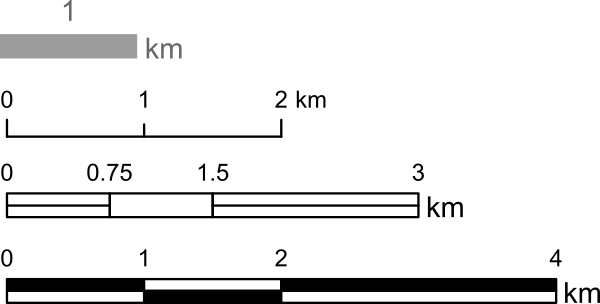
\includegraphics[width=2.60417in,height=\textheight,keepaspectratio]{img/ScaleBar.png}

}

\caption{\label{fig-ScaleBar}Scale bar designs from simplest (top) to
more complex (bottom). Use the simpler design if it's to be placed low
in the visual hierarchy.}

\end{figure}%

\begin{itemize}
\tightlist
\item
  \textbf{Title} and other \textbf{text elements} should be concise. If
  the map is embedded in a report or article, these elements can be
  omitted in favor of figure captions and accompanying text.
\end{itemize}

Let's now look at an improved map layout that applies these principles.
A divergent color scheme is used to highlight variation around a median
income value. County labels have been omitted to reduce visual clutter
and keep the reader's attention focused on the overall spatial pattern
rather than individual counties. The coordinate system preserves
distance, justifying the inclusion of a scale bar. The inset map is
placed low in the hierarchy and could be omitted for audiences familiar
with the region.

\begin{figure}[H]

\centering{


\includegraphics[width=5.5in,height=\textheight,keepaspectratio]{img/Good_map.jpg}

}

\caption{\label{fig-good_map}Example of an \emph{improved} map.}

\end{figure}%

\section{Typefaces and Fonts}\label{typefaces-and-fonts}

Typography plays a subtle but important role in map design. A general
rule is to limit the number of fonts to two: a \textbf{serif} and a
\textbf{sans serif} font.

\begin{figure}[H]

\centering{

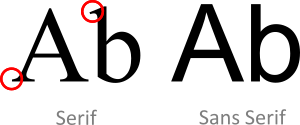
\includegraphics[width=2.08333in,height=\textheight,keepaspectratio]{img/Fonts.png}

}

\caption{\label{fig-serif}Serif fonts are characterized by brush strokes
at the letter tips (circled in red in the figure). Sans Serif fonts are
devoid of brush strokes.}

\end{figure}%

Serif fonts are typically used for natural features such as rivers,
lakes, and mountain ranges. Sans serif fonts are better suited for
human-made features like roads, cities, and administrative boundaries.

Avoid excessive variation in font size unless you are intentionally
creating a hierarchy of labels. Likewise, stick to a single font color
unless you need to distinguish between categories. The following example
shows how thoughtful use of font style and color can improve legibility
and feature separation.

\begin{figure}[H]

\centering{


\includegraphics[width=3.09in,height=\textheight,keepaspectratio]{img/labels.png}

}

\caption{\label{fig-typeset}The lack of typeset differences makes the
map on the left difficult to differentiate county names from lake/river
names. The judicious use of font colors and style on the right
facilitate the separation of features.}

\end{figure}%

\section{Summary}\label{summary-5}

This chapter introduced practical guidelines for creating effective
maps. Good map design helps communicate spatial information clearly
while avoiding unnecessary clutter.

\begin{itemize}
\tightlist
\item
  Establish a clear visual hierarchy, emphasizing the most important
  elements.
\item
  Include only map elements that support the map's purpose.
\item
  Limit the number of colors and ensure that classification choices
  support interpretation.
\item
  Use scale bars and north arrows only when they add value.
\item
  Maintain clear figure-ground contrast so that supporting layers do not
  compete with the primary theme.
\item
  Use fonts consistently and prioritize legibility over decoration.
\end{itemize}

A good map balances visual appeal with communication, ensuring that
every element helps support the map's intended message.

\chapter{Spatial Selection and Vector
Overlays}\label{spatial-selection-and-vector-overlays}

\section{Introduction}\label{introduction-7}

The previous chapters focused on how spatial data are represented,
managed, symbolized, and mapped. We examined how geographic features are
encoded in vector and raster formats, how spatial data are organized,
and how maps can be designed to effectively communicate information. In
this chapter, we shift our attention from representing spatial data to
using it to answer questions.

One of the primary goals of a GIS is to identify, extract, and combine
geographic features in ways that help answer spatial questions.
Sometimes we are interested in features that possess particular
attributes, such as cities with populations greater than 50,000. In
other cases, the question is spatial in nature, such as identifying
cities located within 100 miles of an earthquake event or parcels that
fall within a flood zone. More complex analyses require combining
information from multiple layers to create new geographic features and
attribute relationships.

This chapter introduces three fundamental GIS operations that support
these tasks. We begin with \textbf{attribute queries}, which identifies
features based on information stored in their attribute tables. We then
explore \textbf{spatial queries}, which selects features according to
their spatial relationships with other features. Finally, we examine
\textbf{vector overlay operations}, which combine multiple layers to
generate new spatial and attribute information.

Together, these operations form the foundation of many GIS workflows and
illustrate how geographic data can be queried, filtered, and transformed
to answer spatial questions.

\section{Attribute queries}\label{attribute-queries}

GIS layers often contain rich attribute data that can be queried to
identify features of interest. For example, if a layer represents land
parcels, we might want to select all parcels larger than 2.0 acres or
all parcels zoned for residential use. Such queries are built using
\textbf{comparison operators} and \textbf{Boolean logic}, which allow us
to define the conditions that features must satisfy to be selected.

\subsection{Comparison expressions}\label{comparison-expressions}

Attribute queries are built from \textbf{comparison expressions} that
evaluate whether a condition is true or false. These expressions compare
the value stored in an attribute field to a specified value using
operators such as:

\begin{itemize}
\tightlist
\item
  less than (\texttt{\textless{}}),
\item
  greater than (\texttt{\textgreater{}}),
\item
  equal to (\texttt{=})
\item
  not equal to (\texttt{\textless{}\textgreater{}}).
\end{itemize}

\begin{quote}
In some programming environments (such as R and Python), the equality
condition is expressed using \textbf{two} equal signs, \texttt{==}, and
not one. In such an environment \texttt{x\ =\ 3} is interpreted as
``\emph{pass the value 3 to x}'' and \texttt{x\ ==\ 3} is interpreted as
\emph{``is x equal to 3?''}.
\end{quote}

For example, suppose we want to select all cities with a population
greater than 50,000. Assuming the population field is named
\texttt{POP}, the query expression would be:

\begin{verbatim}
"POP" > 50000
\end{verbatim}

In ArcGIS Pro, one would use the \textbf{Select Layer by Attribute}
tool.

\begin{figure}[H]

\centering{


\includegraphics[width=3.72917in,height=\textheight,keepaspectratio]{img/Select_attribute_1.jpg}

}

\caption{\label{fig-sel1}Attribute queries can be constructed using a
graphical query builder. In this example, comparison operators and
attribute fields are selected from pull-down menus rather than typed
directly as a SQL expression (Figure~\ref{fig-sel2}).}

\end{figure}%

\begin{figure}[H]

\centering{


\includegraphics[width=3.72917in,height=\textheight,keepaspectratio]{img/Select_attribute_2.jpg}

}

\caption{\label{fig-sel2}Many GIS applications allow attribute queries
to be written using SQL syntax. The expression
\texttt{POP\ \textgreater{}\ 50000} evaluates each feature's population
value and selects those exceeding the specified threshold.}

\end{figure}%

\begin{figure}[H]

\centering{

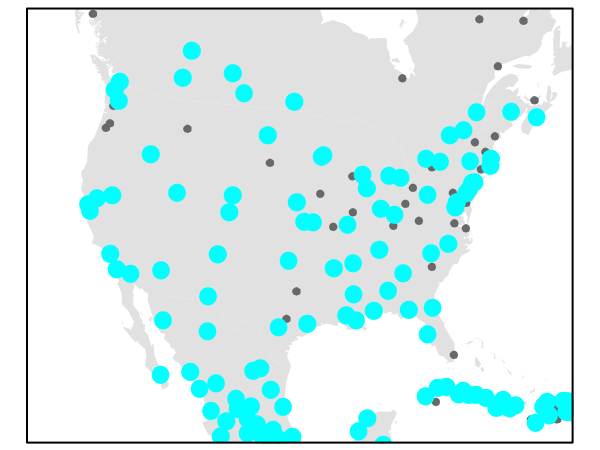
\includegraphics[width=3.125in,height=\textheight,keepaspectratio]{img/Select_cities.png}

}

\caption{\label{fig-sel1_result}Cities with populations greater than
50,000 are selected and highlighted.}

\end{figure}%

\subsection{Boolean Logic}\label{boolean-logic}

A single comparison expression can be used to select features that
satisfy one condition. However, many GIS queries require multiple
conditions. \textbf{Boolean logic} provides a framework for combining
comparison expressions into more complex queries.

Boolean logic combines comparison expressions into statements that
evaluate to either \textbf{TRUE} or \textbf{FALSE} for each feature.
Features for which the statement evaluates to TRUE are selected.

The most common Boolean operators are:

\begin{itemize}
\tightlist
\item
  \texttt{OR}: at least one condition must be true.
\item
  \texttt{AND}: all conditions must be true.
\item
  \texttt{NOT}: reverses a condition, selecting features that do not
  meet it.
\end{itemize}

Suppose we want to select cities with a population greater than 50,000
that are located in the United States. If the country field is labeled
\texttt{FIPS\_CNTRY}, the expression would be:

\begin{verbatim}
`("POP" > 50000) AND ("FIPS_CNTRY" = US)`
\end{verbatim}

Parentheses can be used to control the order in which conditions are
evaluated, just as they are used in arithmetic expressions.

Only features satisfying both conditions would be selected.

\begin{figure}[H]

\centering{

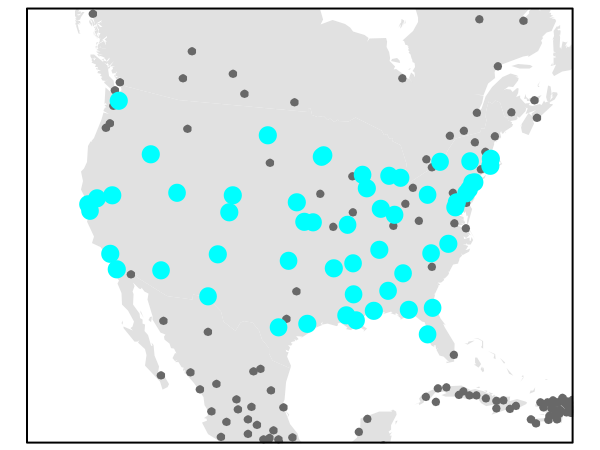
\includegraphics[width=3.125in,height=\textheight,keepaspectratio]{img/Select_cities_2.png}

}

\caption{\label{fig-sel3}Cities satisfying both query conditions (POP
\textgreater{} 50000 AND FIPS\_CNTRY == US) are highlighted. The Boolean
operator AND requires that both conditions evaluate to TRUE before a
feature is selected.}

\end{figure}%

\section{Spatial queries}\label{spatial-queries}

Whereas attribute queries select features based on information stored in
an attribute table, *\textbf{spatial queries} select features based on
their geographic relationship to other features. In ArcGIS Pro, these
operations are implemented through the \textbf{Select Layer by Location}
tool. GIS software evaluates these relationships using feature geometry
rather than attribute values.

Spatial relationships can take many forms, including:

\begin{itemize}
\tightlist
\item
  \textbf{Adjacency}: features that share a boundary
\item
  \textbf{Containment}: features that are entirely within another
  feature
\item
  \textbf{Intersection}: features that overlap or touch one another
\item
  \textbf{Distance}: features within a specified distance of another
  feature
\end{itemize}

For example, suppose we want to identify cities located within 100 miles
of recorded earthquake events. Because this relationship is not
typically stored as an attribute in either layer, GIS evaluates the
spatial relationship between the city and earthquake features to
determine which cities satisfy the selection criterion.

\begin{figure}[H]

\centering{


\includegraphics[width=3.125in,height=\textheight,keepaspectratio]{img/Select_location_1.jpg}

}

\caption{\label{fig-loc1}A \emph{Select Layer by Location} tool is used
to identify features that satisfy a specified spatial relationship. In
this example, cities are selected if they occur within a defined
distance of earthquake events.}

\end{figure}%

This generates the following selection:

\begin{figure}[H]

\centering{


\includegraphics[width=3.125in,height=\textheight,keepaspectratio]{img/Cities_earthquakes.png}

}

\caption{\label{fig-loc1_map}Cities located within the specified
distance of earthquake events are selected and highlighted. This
illustrates the result of a spatial query based on proximity.}

\end{figure}%

\section{Vector overlay operations}\label{vector-overlay-operations}

Vector overlay operations combine information from two or more layers to
create a new output layer. Unlike query operations, which simply select
existing features, overlay operations generate new geometries and
attribute relationships based on spatial overlap. Three common polygon
overlay operations are \textbf{Union}, \textbf{Intersect} and
\textbf{Clip}.

\subsection{Union}\label{union}

\textbf{Union} combines two polygon layers and retains all features from
both input layers. Areas of overlap are split into new polygons defined
by the boundaries of both layers. The output layer typically contains
more polygons than either input layer alone and inherits attributes from
both sources.

\begin{figure}[H]

\centering{


\includegraphics[width=5in,height=\textheight,keepaspectratio]{img/Union.png}

}

\caption{\label{fig-union}A Union operation preserves the complete
geometry of both input layers. Areas of overlap are subdivided into new
polygons that inherit attributes from both layers (e.g., s1 and c1),
while non-overlapping areas retain only the attributes of their original
layer. The resulting output layer typically contains more polygons than
either input layer.}

\end{figure}%

\subsection{Intersect}\label{intersect}

\textbf{Intersect} combines two polygon layers and outputs only the
areas where features from both layers overlap. The resulting polygons
inherit attributes from both input layers, while all non-overlapping
areas are excluded.

\begin{figure}[H]

\centering{


\includegraphics[width=5in,height=\textheight,keepaspectratio]{img/Intersect.png}

}

\caption{\label{fig-intersect}An Intersect operation creates an output
layer composed only of areas where the two input layers overlap. Each
resulting polygon inherits attributes from both input layers. Features
that do not participate in an overlap are omitted from the output.}

\end{figure}%

\subsection{Clip}\label{clip}

\textbf{Clip} uses one layer (the \textbf{clip layer}) to
\emph{cookie-cut} another layer (the \textbf{input layer}). The result
is a subset of the input layer restricted to the area defined by the
clip layer, and only the attributes of the input layer are retained. In
many GIS applications, \textbf{Clip} is implemented as a dedicated tool.
However, conceptually it can be viewed as a special type of overlay
operation in which the clip layer contributes only its boundary geometry
and not its attributes. Some software environments implement clipping
through more general overlay operations like \emph{Intersect} rather
than as a separate tool.

\begin{figure}[H]

\centering{


\includegraphics[width=5in,height=\textheight,keepaspectratio]{img/Clip.png}

}

\caption{\label{fig-clip}A Clip operation restricts the input layer to
the area enclosed by the clip layer. The output retains only the
geometry and attributes of the input layer; the clip layer serves solely
as a spatial boundary and does not contribute attributes to the output.}

\end{figure}%

\section{Summary}\label{summary-6}

This chapter introduced fundamental GIS operations used to query and
combine vector data.

\begin{itemize}
\tightlist
\item
  \textbf{Attribute} queries select features based on conditions applied
  to values stored in an attribute table. They are built using
  comparison expressions and Boolean logic.
\item
  \textbf{Comparison expressions} evaluate whether a condition is true
  or false for each feature, while \textbf{Boolean operators} allow
  multiple conditions to be combined into more complex queries.
\item
  \textbf{Spatial queries} select features based on their geographic
  relationship to other features, such as distance, containment,
  adjacency, or intersection.
\item
  Unlike queries, which identify existing features, \textbf{vector
  overlay operations} create new datasets by combining information from
  multiple layers.
\item
  A \textbf{Union} operation preserves all areas from both input layers
  and combines their attributes where overlaps occur.
\item
  An \textbf{Intersect} operation retains only areas shared by both
  input layers and combines attributes from each layer.
\item
  A \textbf{Clip} operation uses one layer as a spatial boundary to
  extract a subset of another layer while retaining only the attributes
  of the input layer.
\end{itemize}

Attribute queries, spatial queries, and overlay operations form the
foundation of many GIS workflows and provide a framework for extracting,
filtering, and transforming geographic information.

\chapter{Coordinate Systems}\label{chp09_0}

\section{Introduction}\label{introduction-8}

Every GIS dataset is tied to a spatial reference system, which defines
how locations are represented and interpreted. This system may be
arbitrary--such as a 10 m × 10 m sampling grid in a forest plot or the
layout of a soccer field--or it may be geographic, linking spatial
features to positions on the Earth's surface. This chapter focuses on
Earth-based reference systems.

At first glance, representing a location on Earth may seem
straightforward. For example, we might describe Colby College as being
located at a particular latitude and longitude. However, before
coordinates can be assigned, we must first answer a more fundamental
question:

\begin{quote}
What model of the Earth are those coordinates based on?
\end{quote}

The Earth is not a perfect sphere, nor is it perfectly smooth. Its
shape, gravitational field, and curvature must all be approximated
before locations can be measured and mapped. Different approximations
can produce slightly different coordinate values for the same physical
location. Understanding these approximations is essential when working
with spatial data from different sources.

Earth-based coordinate systems generally fall into two broad categories:

\begin{itemize}
\tightlist
\item
  \textbf{Geographic Coordinate Systems (GCS)}, which locate positions
  on the curved surface of the Earth using latitude and longitude.
\item
  \textbf{Projected Coordinate Systems (PCS)}, which transform the
  curved Earth onto a flat surface suitable for mapping and spatial
  analysis.
\end{itemize}

In this chapter, we begin by examining how locations are defined on the
Earth through geographic coordinate systems. We then explore projected
coordinate systems and the distortions introduced when translating a
curved surface onto a flat map. Finally, we examine how different
coordinate systems affect spatial measurements such as area, distance,
direction, and shape.

\section{Geographic Coordinate
Systems}\label{geographic-coordinate-systems}

\subsection{Latitude and Longitude}\label{latitude-and-longitude}

A geographic coordinate system (GCS) identifies locations on the Earth's
surface using two angular measurements: \textbf{latitude} and
\textbf{longitude}. Unlike projected coordinate systems, which measure
location using linear units such as meters or feet, a geographic
coordinate system measures position using angles referenced to the
Earth's center.

Latitude and longitude are defined relative to two reference planes:

\begin{itemize}
\tightlist
\item
  the \textbf{equatorial plane}, which divides Earth into Northern and
  Southern Hemispheres,
\item
  the \textbf{prime meridian plane}, which passes through Greenwich,
  England and divides Earth into Eastern and Western Hemispheres.
\end{itemize}

A location on Earth can therefore be uniquely identified by a pair of
values: latitude and longitude.

Latitude measures how far north or south a location lies relative to the
equator. It ranges from 0° at the equator to 90° at the North Pole and
-90° at the South Pole.

Longitude measures how far east or west a location lies relative to the
prime meridian. Longitude ranges from 0° at the prime meridian to +180°
eastward and -180° westward.

\begin{figure}[H]

\centering{


\includegraphics[width=3.72917in,height=\textheight,keepaspectratio]{img/lat_vs_lon.png}

}

\caption{\label{fig-latlong}Latitude and longitude provide a geographic
framework for locating positions on the Earth's surface. Latitude
measures angular distance north or south of the equator (left), whereas
longitude measures angular distance east or west of the prime meridian
(right). The red lines indicate the 0° reference locations from which
each measurement is made.}

\end{figure}%

For example, Colby College is located at approximately 44.5° North and
69.5° West. In many GIS applications, north and east coordinates are
assigned \textbf{positive values}, whereas south and west coordinates
are assigned \textbf{negative values}. Thus, the same location can be
represented as (+44.5°, -69.5°).

\begin{figure}[H]

\centering{


\includegraphics[width=3.64583in,height=\textheight,keepaspectratio]{img/Colby_location_sphere.jpg}

}

\caption{\label{fig-sphere_slice}Latitude and longitude are measured as
angles from the Earth's center rather than as linear distances along its
surface. Latitude is referenced to the equatorial plane, while longitude
is referenced to the prime meridian plane.}

\end{figure}%

One consequence of using latitude and longitude is that the units are
angular rather than linear. As a result, a one-degree change in
longitude does not correspond to the same ground distance everywhere on
Earth. This complicates distance and area measurements and motivates the
use of projected coordinate systems introduced later in this chapter.

\subsection{Why Coordinate Systems
Differ}\label{why-coordinate-systems-differ}

At first glance, a geographic coordinate system appears straightforward:
every location on Earth can be identified by a latitude and longitude
value. It is therefore tempting to assume that a given location should
always have the same coordinates. In practice, however, this is not the
case. The same physical location can have different latitude and
longitude values depending on the coordinate system used.

Why does this happen? The answer lies in how the Earth is represented
mathematically. Latitude and longitude measurements are referenced to a
model of the Earth, but the Earth is not a perfect sphere. It is
slightly flattened at the poles, has an irregular gravitational field,
and exhibits subtle variations in shape. To create coordinate systems
that can be used consistently around the world, these complexities must
be \emph{approximated} using mathematical models. Different
approximations lead to different coordinate systems.

The next sections introduce the three key concepts that form the
foundation of modern geographic coordinate systems:

\begin{itemize}
\tightlist
\item
  the \textbf{ellipsoid}, a mathematical model used to approximate the
  Earth's shape;
\item
  the \textbf{geoid}, a model representing the Earth's gravitational
  surface; and
\item
  the \textbf{datum}, which defines how the ellipsoid is aligned with
  the Earth.
\end{itemize}

Understanding these concepts is essential because coordinate values are
meaningful only when the underlying geographic coordinate system is
known. Two datasets may describe the same location using slightly
different coordinate values if they are referenced to different datums.

\subsection{Sphere and Ellipsoid}\label{sphere-and-ellipsoid}

To assign coordinates to locations on Earth, we first need a
mathematical model of the planet's shape. The simplest model treats the
Earth as a perfect sphere. A sphere is attractive because its geometry
is easy to work with mathematically and provides a reasonable
approximation for many small-scale maps and global visualizations.
However, the Earth is not perfectly spherical. Measurements made from
satellites and geodetic surveys show that the Earth is slightly
flattened at the poles and bulges outward at the equator.

To better represent the Earth's shape, geographic coordinate systems
typically use an ellipsoid rather than a sphere. An ellipsoid can be
thought of as a slightly compressed sphere whose shape is defined by two
radii:

\begin{itemize}
\tightlist
\item
  The \textbf{semi-major axis}, which represents the equatorial radius,
  and
\item
  The \textbf{semi-minor axis}, which represents the polar radius.
\end{itemize}

These dimensions provide a closer approximation of the Earth's shape and
improve the accuracy of geographic coordinates and spatial measurements.
Figure~\ref{fig-ellipse_axes0} illustrates the two axes used to define
an ellipsoid.

\begin{figure}[H]

\centering{

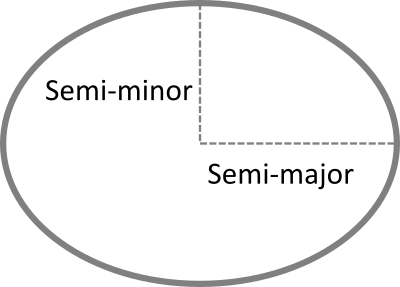
\includegraphics[width=2.08333in,height=\textheight,keepaspectratio]{img/Ellipsoid.png}

}

\caption{\label{fig-ellipse_axes0}An ellipsoid is defined by two radii:
the semi-major axis, which measures the equatorial radius, and the
semi-minor axis, which measures the polar radius. If the two radii are
equal, the ellipsoid becomes a perfect sphere.}

\end{figure}%

The Earth is not a perfect sphere. Its rotation produces a centrifugal
effect that causes the planet to bulge slightly at the equator and
flatten at the poles. As a result, the Earth's equatorial radius is
approximately 21 km longer than its polar radius. While this difference
is small relative to the Earth's overall size, it is large enough to
affect spatial measurements and coordinate calculations. Consequently,
modern geographic coordinate systems typically represent the Earth as an
ellipsoid rather than a sphere.

\begin{figure}

\begin{minipage}[t]{0.50\linewidth}

\begin{figure}[H]

\centering{


\includegraphics[width=1.5625in,height=\textheight,keepaspectratio]{img/globe_0_0_center.png}

}

\caption{\label{fig-sphere_ellipse-1}A spherical Earth model assumes
that the Earth's radius is identical in all directions. Although
convenient mathematically, it does not fully capture the Earth's true
shape.}

\end{figure}%

\end{minipage}%
%
\begin{minipage}[t]{0.50\linewidth}

\begin{figure}[H]

\centering{


\includegraphics[width=1.92708in,height=\textheight,keepaspectratio]{img/globe_0_0_center_wide.png}

}

\caption{\label{fig-sphere_ellipse-2}An ellipsoidal Earth model accounts
for the Earth's equatorial bulge and polar flattening, providing a more
accurate representation than a sphere.}

\end{figure}%

\end{minipage}%

\end{figure}%

For many applications, the difference between a sphere and an ellipsoid
is small. However, when high positional accuracy is required, the
ellipsoidal model provides more accurate coordinate and distance
calculations.

Modern geodetic measurements derived from satellites and ground-based
surveys have produced highly accurate estimates of the Earth's
dimensions. For example, the WGS84 ellipsoid uses a semi-major axis of
6,378,137 meters and a semi-minor axis of 6,356,752 meters. Although the
difference between these radii represents only a small fraction of the
Earth's overall size, it is sufficient to affect coordinate calculations
and distance measurements.

For many mapping applications these differences are negligible. However,
when measurements span large distances, the choice of a spherical or
ellipsoidal Earth model can produce measurable discrepancies.
Figure~\ref{fig-dist_diff} illustrates these differences by comparing
distances computed on a sphere with those computed on an ellipsoid. In
some cases, the discrepancy approaches 20 km.

\begin{figure}[H]

\centering{

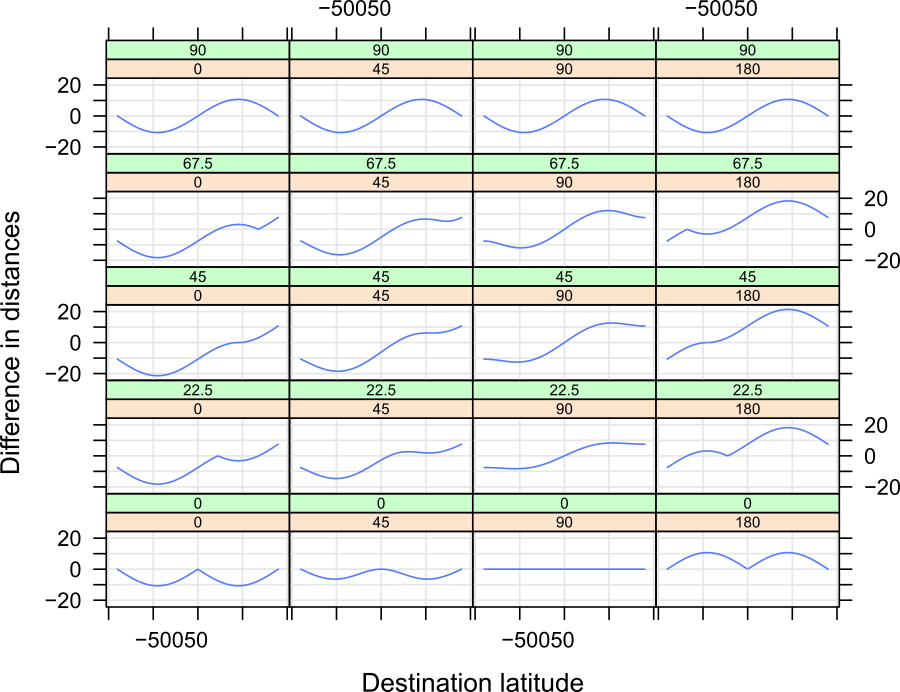
\includegraphics[width=6.25in,height=\textheight,keepaspectratio]{img/Ellipsoid_vs_sphere_distances.png}

}

\caption{\label{fig-dist_diff}Differences in distance measurements
computed on a sphere versus an ellipsoid. The discrepancies vary with
latitude and direction and can approach 20 km for some long-distance
measurements. These results illustrate why modern geographic coordinate
systems typically adopt an ellipsoidal Earth model.}

\end{figure}%

Although the ellipsoid provides a much better approximation of the
Earth's shape than a sphere, it remains a mathematical simplification.
The Earth is not a perfectly smooth surface and its mass is not
distributed uniformly. Variations in the Earth's density create small
differences in its gravitational field, causing the Earth's true shape
to deviate from a simple ellipsoid. To account for these variations,
geodesists introduce another model of the Earth known as the
\textbf{geoid}.

\subsection{Geoid}\label{geoid}

The \textbf{geoid} is a model of the Earth's gravitational surface.
Unlike the smooth and mathematically defined ellipsoid, the geoid
contains subtle undulations caused by variations in the Earth's gravity
field. These variations arise because the Earth's mass is not
distributed uniformly throughout the planet. Although the deviations are
small relative to the Earth's overall size, they can be measured and are
important in high-accuracy positioning and surveying applications.

It is important to distinguish the geoid from the Earth's topography. In
this context, we are not concerned with mountains, valleys, or ocean
trenches. Instead, we can imagine the Earth completely covered by a
motionless ocean. The resulting surface, shaped only by gravity,
approximates the geoid. Differences between the geoid and ellipsoid are
therefore caused by variations in the Earth's gravity field rather than
by surface terrain.

\begin{figure}[H]

\centering{


\includegraphics[width=2.08333in,height=\textheight,keepaspectratio]{img/geoid.png}

}

\caption{\label{fig-geoid}The geoid is a gravity-based reference surface
that approximates mean sea level worldwide. Its undulations reflect
variations in the Earth's gravitational field caused by non-uniform mass
distribution within the planet. The vertical variations are greatly
exaggerated (4000×) to make them visible.}

\end{figure}%

The Earth is not a static body. Tectonic plate motion, changes in the
distribution of water and ice, and variations within the Earth's
interior can cause small changes in the Earth's shape and gravitational
field over time. As a result, geodetic reference systems are
periodically updated to maintain positional accuracy. The science of
measuring and modeling the Earth's shape, orientation, and gravity field
is known as \textbf{geodesy}.

\subsection{Datum}\label{datum}

We now have two different models of the Earth. The \textbf{ellipsoid}
provides a mathematically convenient representation of the Earth's
shape, whereas the \textbf{geoid} provides a more realistic
representation of the Earth's gravitational surface. Because geographic
coordinates are computed on an ellipsoid, we must specify how that
ellipsoid is positioned relative to the geoid. This alignment defines a
\textbf{datum}. A datum therefore serves as a bridge between the
mathematical model used for calculations and the physical Earth it is
intended to represent

The alignment can be:

\begin{itemize}
\tightlist
\item
  \textbf{Local}, where the ellipsoid is closely fitted to the geoid at
  a specific location (e.g., Kansas), or
\item
  \textbf{Geocentric}, where the ellipsoid is aligned with the Earth's
  center of mass.
\end{itemize}

\begin{figure}[H]

\centering{


\includegraphics[width=5.72917in,height=\textheight,keepaspectratio]{img/datum.png}

}

\caption{\label{fig-datum}A datum is created by defining how an
ellipsoid is aligned relative to the geoid. Different alignments produce
different coordinate systems and can yield different coordinate values
for the same physical location.}

\end{figure}%

Historically, many datums were designed to provide the best possible fit
for a particular region rather than for the entire Earth. These are
known as \textbf{local datums}.

\subsubsection{Local Datum}\label{local-datum}

\begin{figure}[H]

\centering{

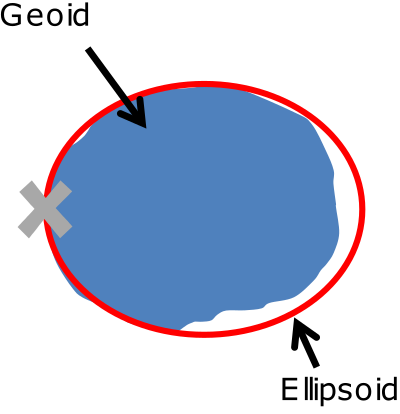
\includegraphics[width=2.08333in,height=\textheight,keepaspectratio]{img/Datum_local.png}

}

\caption{\label{fig-datum_local}A local datum aligns the ellipsoid to
provide the best fit within a specific region. Positional accuracy is
maximized near the point of alignment but may decrease farther away.}

\end{figure}%

There are many local datums, both historical and modern. The choice of
datum is typically driven by geographic context. For example:

\begin{itemize}
\tightlist
\item
  \textbf{NAD27} (North American Datum of 1927) is widely used in the
  U.S., especially in older maps.
\item
  \textbf{ED50} (European Datum of 1950) is common in Western Europe.
\item
  \textbf{WGS72} (World Geodetic System 1972) was developed for global
  use by the U.S. Department of Defense.
\end{itemize}

Advances in satellite technology made it possible to construct datums
centered on the Earth's center of mass rather than optimized for a
particular region. These are known as \textbf{geocentric datums}.

\subsubsection{Geocentric Datum}\label{geocentric-datum}

\begin{figure}[H]

\centering{

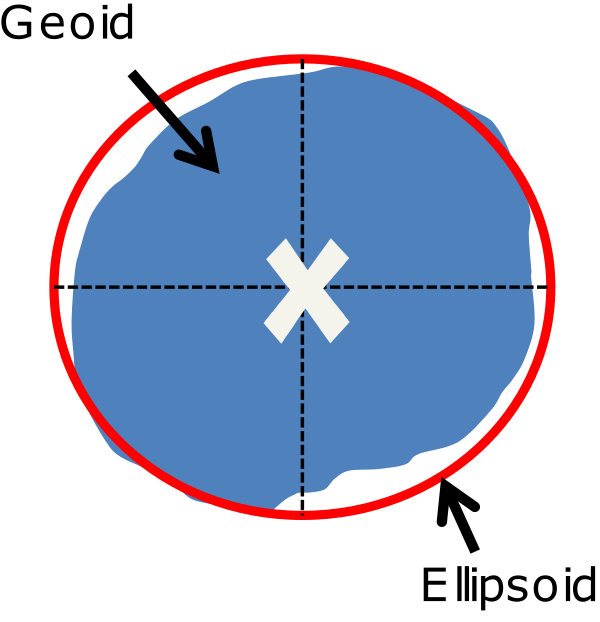
\includegraphics[width=2.08333in,height=\textheight,keepaspectratio]{img/Datum_geocentric.png}

}

\caption{\label{fig-datum_geocentric}A geocentric datum aligns the
ellipsoid with the Earth's center of mass. This produces a coordinate
system suitable for global positioning and satellite navigation.}

\end{figure}%

Modern datums typically use a geocentric alignment. Examples include:

\begin{itemize}
\tightlist
\item
  \textbf{NAD83} (North American Datum of 1983)
\item
  \textbf{ETRS89} (European Terrestrial Reference System 1989)
\item
  \textbf{WGS84} (World Geodetic System 1984)
\end{itemize}

Most modern datums use either the WGS84 or GRS80 ellipsoid, which have
nearly identical dimensions: a semi-major axis of 6,378,137 meters and a
semi-minor axis of 6,356,752 meters.

We can now assemble the components of a geographic coordinate system: an
ellipsoid provides the mathematical model of the Earth, and a datum
specifies how that model is aligned with the Earth.

\subsection{Building the Geographic Coordinate
System}\label{building-the-geographic-coordinate-system}

We can now assemble the components of a \textbf{Geographic Coordinate
System (GCS)}. A GCS is created by combining:

\begin{enumerate}
\def\labelenumi{\arabic{enumi}.}
\tightlist
\item
  an \textbf{ellipsoid}, which provides a mathematical model of the
  Earth's shape, and
\item
  a \textbf{datum}, which defines how that ellipsoid is aligned with the
  Earth.
\end{enumerate}

Together, these components provide the reference framework used to
assign latitude and longitude coordinates to locations on the Earth's
surface.

Because different ellipsoids and datums may be used, the same physical
location can have different latitude and longitude coordinates under
different geographic coordinate systems. For this reason, it is
essential to know the coordinate system associated with a dataset before
combining it with other spatial data.

For example, a point recorded in NAD27 will typically have slightly
different latitude and longitude values when expressed in NAD83, even
though the physical location has not changed. The difference arises
because the two coordinate systems use different datum definitions.
Figure~\ref{fig-GCS_offsets} illustrates this effect using the location
of the Colby College flagpole.

\begin{figure}[H]

\centering{


\includegraphics[width=5.625in,height=\textheight,keepaspectratio]{img/GCS_diff_coord_values.png}

}

\caption{\label{fig-GCS_offsets}The same physical location represented
in two different geographic coordinate systems (NAD83 on the left and
NAD27 on the right). Although the flagpole has not moved, differences in
datum definitions cause its coordinates to shift slightly between
reference systems.}

\end{figure}%

For example, a point recorded as 44.56698° N, 69.65939° W in NAD27 may
appear as 44.56704° N, 69.65888° W in NAD83. Although the coordinate
values differ, both refer to the same physical location. Without proper
metadata, these differences can lead to misaligned features when
datasets from multiple coordinate systems are combined.

A useful analogy is temperature measurement. Water freezes at 0°C, 32°F,
and 273.15 K. The numeric values differ, but the physical phenomenon is
identical. Likewise, the same location can have different coordinate
values under different geographic coordinate systems even though the
location itself has not changed.

Modern GIS software stores coordinate system information as metadata and
can automatically transform data between many common geographic
coordinate systems. Nevertheless, identifying the correct coordinate
system remains an essential first step in any GIS workflow.

\section{Projected Coordinate
Systems}\label{projected-coordinate-systems}

\subsection{What is a Projected Coordinate
System?}\label{what-is-a-projected-coordinate-system}

A \textbf{Projected Coordinate System (PCS)} provides a framework for
identifying locations on a \textbf{flat} surface. Unlike a Geographic
Coordinate System, which uses angular coordinates (latitude and
longitude), a PCS uses \textbf{Cartesian coordinates} measured in linear
units such as meters or feet. A projected coordinate system consists of
an origin, an x-axis, a y-axis, and a coordinate grid formed by lines
that intersect at right angles.

\begin{quote}
FYI: A projected coordinate system is always built upon an underlying
Geographic Coordinate System (GCS). The projection defines how
coordinates are transformed from the curved Earth to a flat surface, but
the ellipsoid and datum used by the PCS are inherited from its parent
GCS. As a result, the same projection method can produce slightly
different coordinate values and spatial measurements when paired with
different geographic coordinate systems. For example, a UTM projection
based on NAD83 will not produce exactly the same coordinates as a UTM
projection based on WGS84, even though both use the same projection
method.
\end{quote}

\subsection{Why Do We Need
Projections?}\label{why-do-we-need-projections}

Latitude and longitude provide a convenient way to locate positions on
the Earth's surface, but they are less well suited for measuring spatial
properties such as distance, area, and direction. Because the Earth is
curved, angular coordinate systems do not naturally provide the planar
framework needed for mapping and analytical tasks.

Projected coordinate systems became widely adopted because many
surveying and engineering measurements were traditionally performed on a
plane. Even after the introduction of digital computers, projected
coordinate systems remained important because measurements of distance,
area, and direction could often be computed more efficiently on a plane
than on a curved Earth model. As a result, projected coordinate systems
became the standard framework for many GIS operations and mapping
applications.

However, transforming locations from a curved Earth to a flat map cannot
be done without introducing some form of \textbf{distortion}. A map
projection provides the mathematical transformation needed to convert
locations from a Geographic Coordinate System (GCS) to a Projected
Coordinate System (PCS). Every projection introduces distortions that
affect one or more spatial properties, including \textbf{shape},
\textbf{area}, \textbf{distance}, and \textbf{direction}.

\begin{quote}
Modern GIS software is capable of performing measurements directly on an
ellipsoid using geodesic methods. These approaches often provide more
accurate results over large distances and geographic extents.
Nevertheless, projected coordinate systems remain widely used because of
their computational efficiency. Geodesic measurements are discussed
later in this chapter (Section~\ref{sec-geodesic}).
\end{quote}

\section{Spatial Properties}\label{spatial-properties}

All map projections introduce distortion because a curved Earth cannot
be represented on a flat surface without alteration. The four spatial
properties most affected by projection are: \textbf{shape},
\textbf{area}, \textbf{distance} and \textbf{direction}. Different
projections are designed to preserve one or more of these properties
while accepting distortions in others.

A projection that preserves shape is called \textbf{conformal}. A
projection that preserves area is called \textbf{equal-area}. A
projection that preserves distance is called \textbf{equidistant}. A
projection that preserves direction is called \textbf{azimuthal}.

\begin{quote}
Many GIS applications include these properties directly in the
projection name. For example, \emph{Albers Equal Area} prioritizes area
preservation, whereas \emph{Lambert Conformal Conic} prioritizes shape
preservation.
\end{quote}

\subsection{Shape}\label{shape}

A map projection preserves shape when local angles and geometric forms
remain unchanged. Such projections are called conformal projections.
While small features maintain their appearance, the preservation of
shape often comes at the expense of area, distance, or both.

\subsection{Area}\label{area}

A map projection preserves area when the relative size of mapped
features remains proportional to their true size on the Earth. Such
projections are called equal-area projections. Equal-area projections
are commonly used for statistical mapping because they prevent regions
from appearing larger or smaller than they actually are.

\subsection{Distance}\label{distance}

A map projection preserves distance when distances measured on the map
correspond to true distances on the Earth. Such projections are called
equidistant projections. However, distance preservation is usually
limited to specific directions, locations, or reference lines rather
than across the entire map.

\subsection{Direction}\label{direction}

A projection preserves direction when bearings measured from a specified
location correspond to true directions on the Earth. Such projections
are often referred to as azimuthal projections. Direction-preserving
projections are commonly used in navigation and aviation applications.

\subsection{Measuring Projection
Distortion}\label{measuring-projection-distortion}

Because every projection represents a compromise among shape, area,
distance, and direction, it is useful to have a way to visualize
distortion. One common approach uses \textbf{Tissot indicatrices (TI)},
which show how a small circle on the Earth is transformed by a map
projection.

The idea is to project a small circle--small enough that distortion
remains nearly uniform across its extent--and examine its transformed
shape on the map.

For example, to evaluate distortion in a Mollweide projection across the
continental U.S., a grid of circles can be generated at regular
latitudinal and longitudinal intervals.

\begin{figure}[H]

\centering{


\includegraphics[width=6.25in,height=\textheight,keepaspectratio]{img/Moll_Tissot.png}

}

\caption{\label{fig-moll_tissot}Tissot indicatrices generated for a
Mollweide projection across the continental United States. Variations in
the size and shape of the indicatrices reveal how projection distortion
changes across geographic space.}

\end{figure}%

Note the varying levels of distortion type and magnitude across the
region. To better understand how a Tissot indicatrix captures these
distortions, let's zoom in on a circle centered at 44.5°N and 69.5°W
(near Waterville Maine):

\begin{figure}[H]

\centering{


\includegraphics[width=4.16667in,height=\textheight,keepaspectratio]{img/Moll_Tissot_Zoom.png}

}

\caption{\label{fig-moll_tissot_zoom}A Tissot indicatrix centered near
Waterville, Maine. The bisque circle represents the undistorted
geometry, whereas the blue ellipse shows the distortion introduced by
the Mollweide projection. The major and minor axes define the principal
directions of scale distortion.}

\end{figure}%

The plot shows a perfect circle (filled in bisque) that would be
expected if no distortion were present. The blue ellipse (the
indicatrix) represents the transformed circle for this particular
projection and location. The green and red lines indicate the magnitude
and orientation of the ellipse's major and minor axes, respectively.
These lines can also be used to assess \textbf{scale distortion}, which
may vary depending on direction (bearing).

\begin{itemize}
\tightlist
\item
  The green line shows the direction of \textbf{maximum scale
  distortion}.
\item
  The red line shows the direction of \textbf{minimum scale distortion}.
\end{itemize}

These directions are sometimes referred to as the \textbf{principal
directions}. In this example, the principal scale values are 1.1293 and
0.8856. A scale value of 1 indicates no distortion; values less than 1
indicate a smaller-than-true scale, and values greater than 1 indicate a
larger-than-true scale.

It's important to note that scale distortion does not necessarily imply
area distortion. In fact, for this projection, area is relatively well
preserved despite directional scale distortion. An estimate of local
area distortion can be obtained by multiplying the two principal scale
values. In this example, the area distortion is 1.0001--effectively
negligible.

The dashed north-south line in the graphic shows the orientation of the
meridian, while the dotted east-west line shows the orientation of the
parallel.

\begin{quote}
It's important to remember that these distortions occur at the center of
the TI and may not reflect distortion across the entire region covered
by the TI circle.
\end{quote}

Tissot indicatrices provide a compact way to visualize how a projection
alters shape, area, distance, and direction, making them a valuable tool
for evaluating projection performance.

No map projection can perfectly preserve shape, area, distance, and
direction simultaneously. Instead, different projections are designed to
minimize or distribute distortion in different ways. The next section
introduces three broad families of map projections--planar, cylindrical,
and conical--and examines how each attempts to manage distortion across
the Earth's surface.

\section{Projection Families}\label{projection-families}

Different projection families contact the Earth in different ways and
therefore distribute distortion differently across a map. Three common
projection families are \textbf{planar}, \textbf{cylindrical}, and
\textbf{conical}.

\subsection{Planar Projections}\label{planar-projections}

A \textbf{planar projection} maps the Earth's surface onto a flat plane.
The plane may touch the globe at a single point (\textbf{tangent} case)
or intersect the globe along a circle (\textbf{secant} case). Planar
projections are also commonly referred to as \textbf{azimuthal
projections}.

Distortion is generally smallest near the point or line of contact and
increases with distance from it.

\begin{figure}[H]

\centering{

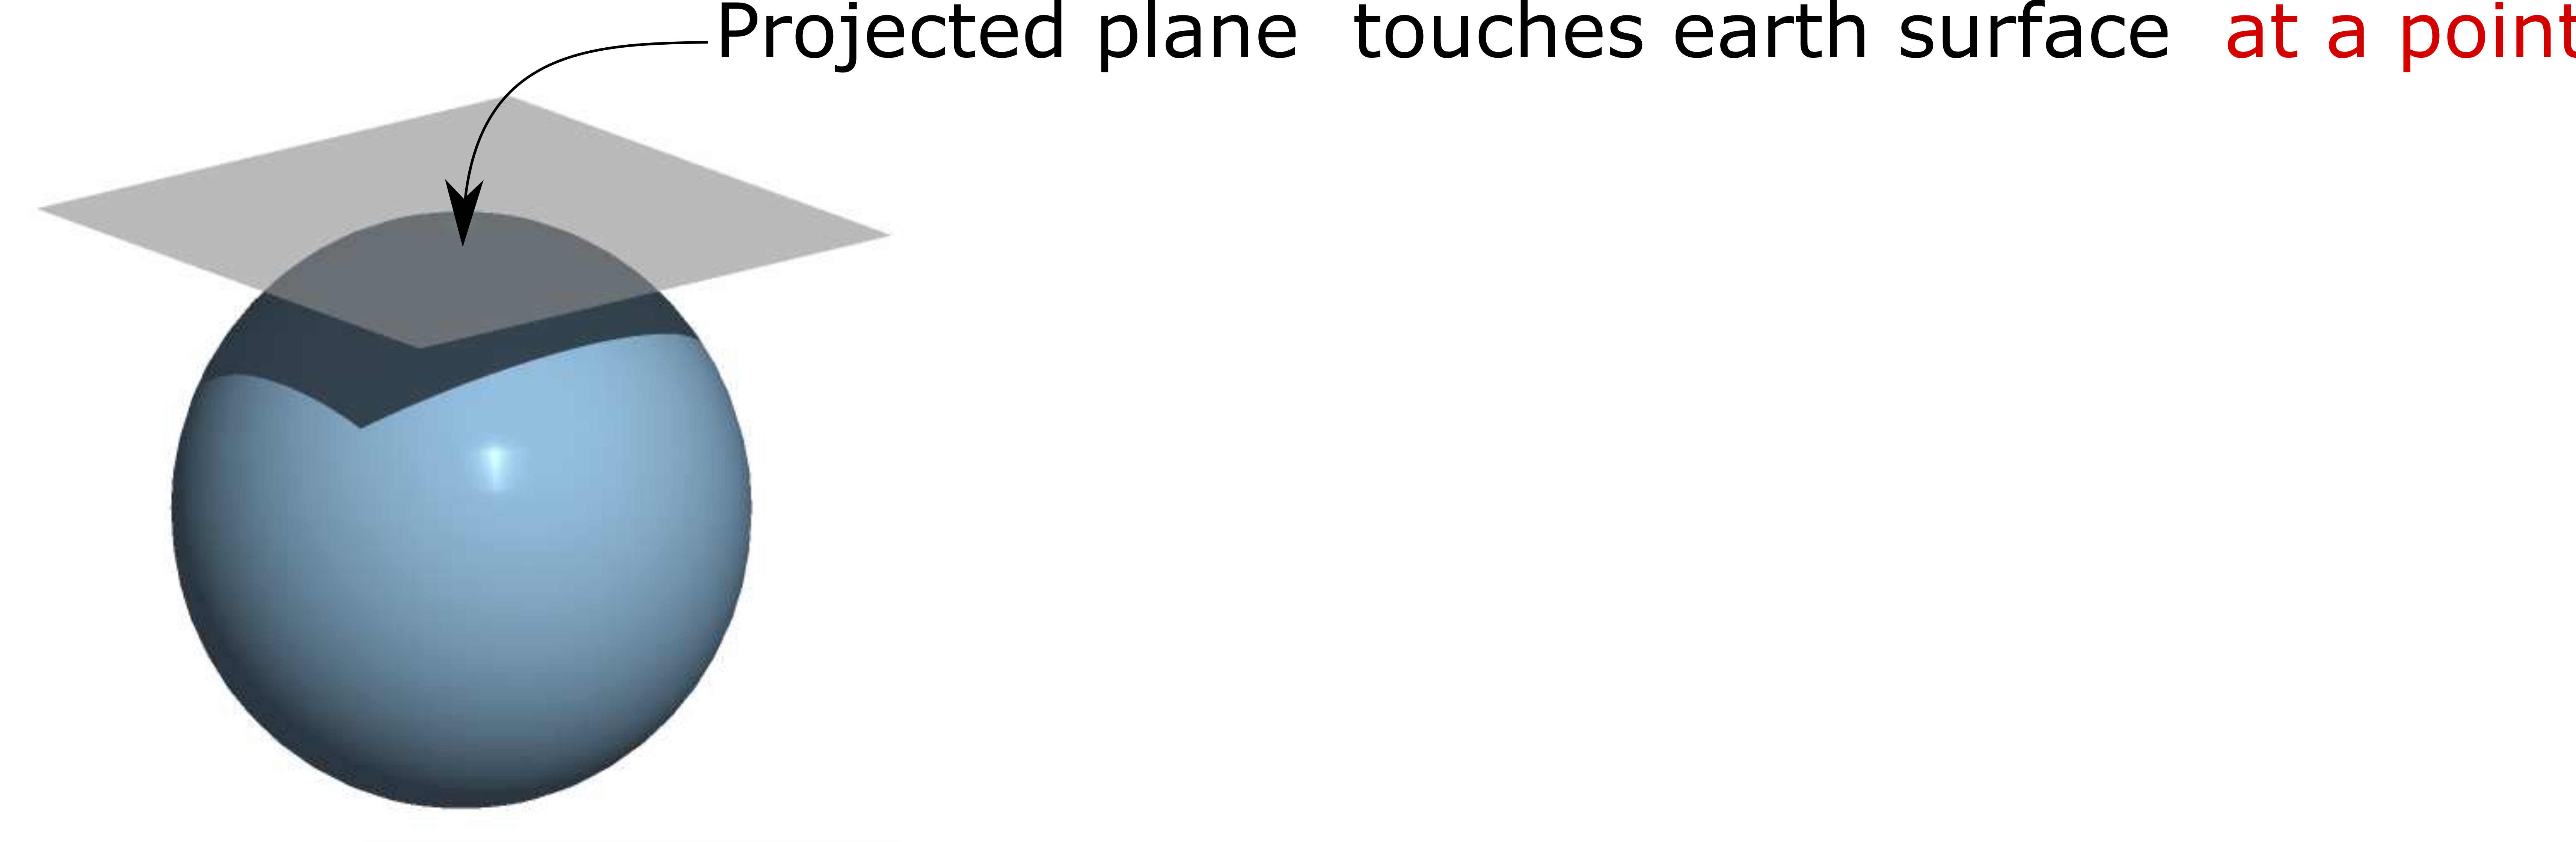
\includegraphics[width=6.25in,height=\textheight,keepaspectratio]{img/Planar_projection_tangent.png}

}

\caption{\label{fig-tangent}A tangent planar projection. The projection
surface touches the globe at a single point, where distortion is
minimized.}

\end{figure}%

\begin{figure}[H]

\centering{

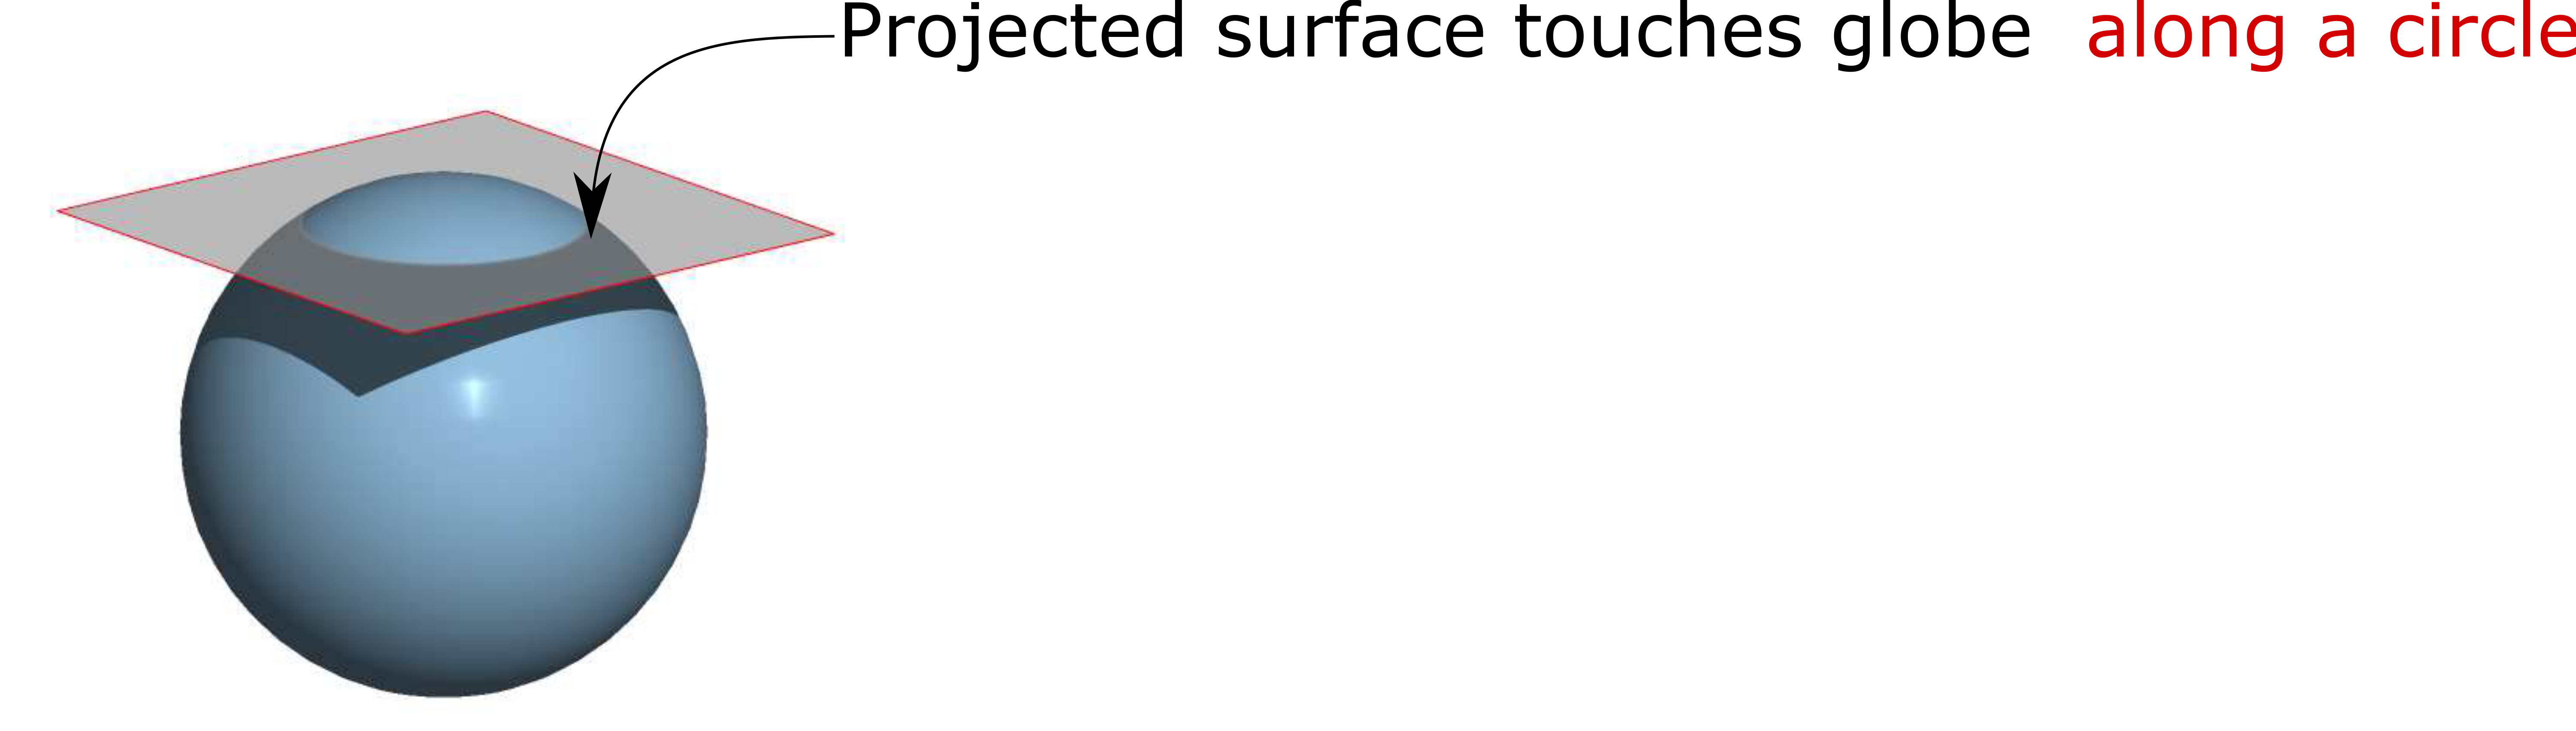
\includegraphics[width=6.25in,height=\textheight,keepaspectratio]{img/Planar_projection_secant.png}

}

\caption{\label{fig-secant}A secant planar projection. The projection
surface intersects the globe along a circle, reducing distortion over a
larger region than the tangent case.}

\end{figure}%

Although planar projections are often used for polar regions, the point
of contact can be placed anywhere on the globe. When the projection is
centered on a location other than a pole, it is referred to as an
\textbf{oblique} planar projection.

\begin{figure}[H]

\centering{


\includegraphics[width=5.20833in,height=\textheight,keepaspectratio]{img/Planar_Examples.png}

}

\caption{\label{fig-planar_examples}Examples of three planar
projections: orthographic (left), gnomonic (center) and equidistant
(right). Different planar projections preserve different spatial
properties and vary in the geographic extent they can represent
effectively.}

\end{figure}%

\subsection{Cylindrical Projection}\label{cylindrical-projection}

A cylindrical projection maps Earth's surface onto a cylinder, which is
then unrolled into a flat map. The cylinder may touch the globe along a
single line of tangency (a \textbf{tangent} case) or intersect the globe
along two lines (a \textbf{secant} case).

\begin{figure}[H]

\centering{

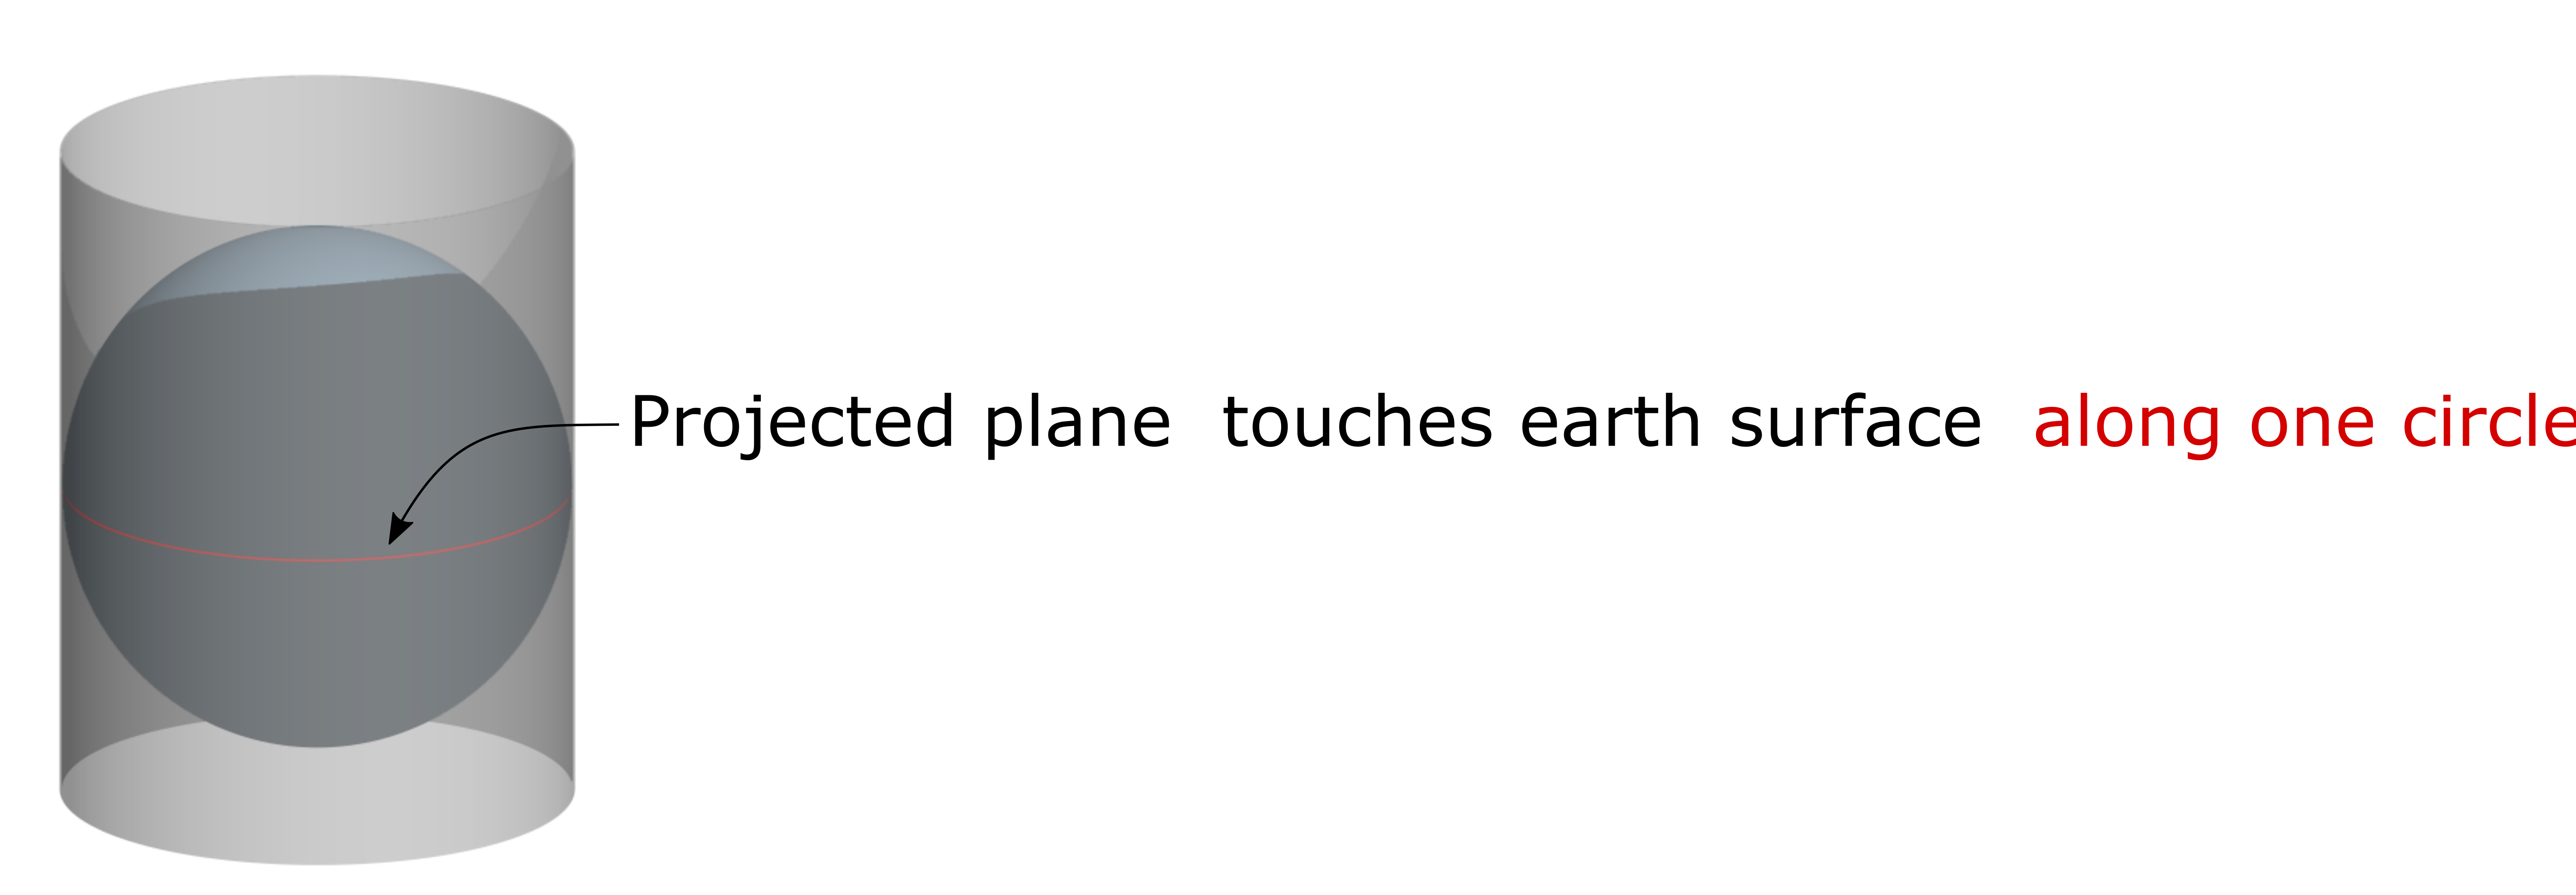
\includegraphics[width=5.98958in,height=\textheight,keepaspectratio]{img/Cylindrical_projection_tangent.png}

}

\caption{\label{fig-tangent2}A tangent cylindrical projection. The
projection surface touches the globe along a single line, where
distortion is minimized.}

\end{figure}%

\begin{figure}[H]

\centering{

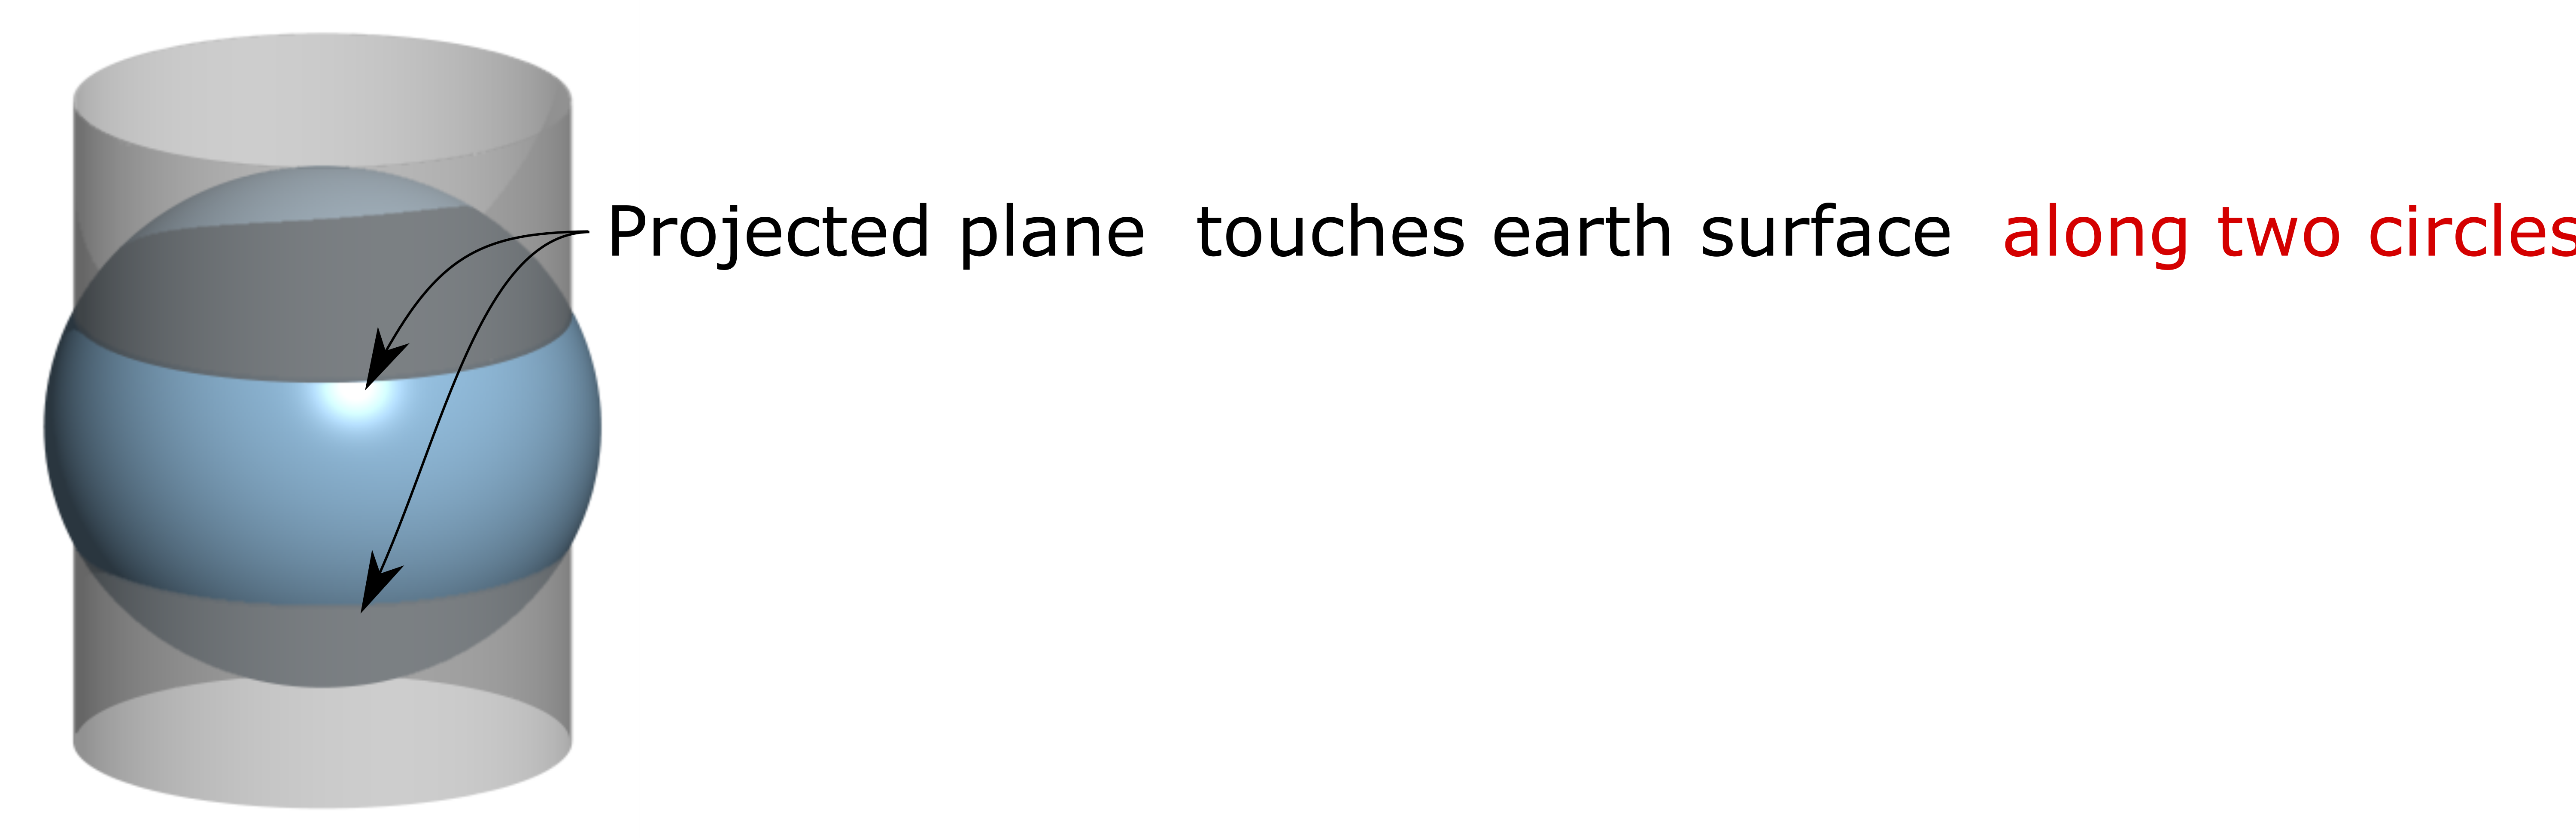
\includegraphics[width=5.98958in,height=\textheight,keepaspectratio]{img/Cylindrical_projection_secant.png}

}

\caption{\label{fig-secant2}A secant cylindrical projection. The
projection surface intersects the globe along two lines, reducing
distortion over a larger region than the tangent case.}

\end{figure}%

Distortion is minimized along the tangent or secant lines and generally
increases with distance from them.

The cylinder is typically tangent to the equator, but it can also be
oblique. A special case is the \textbf{transverse aspect}in which the
cylinder is tangent to a meridian rather than the equator. This approach
forms the basis of the \textbf{Universal Transverse Mercator (UTM)}
system and many \textbf{State Plane coordinate systems}.

The UTM system divides the globe into 60 zones, each 6° wide. Because
each zone covers a relatively small geographic extent, distortion
remains low. For example, Maine is commonly mapped using \textbf{UTM
Zone 19 North}. UTM coordinates may be referenced to different datums,
including NAD27, NAD83, and WGS84.

\begin{figure}[H]

\centering{


\includegraphics[width=6.25in,height=\textheight,keepaspectratio]{img/Cylindrical_Examples.png}

}

\caption{\label{fig-cylindrical_examples}Examples of two cylindrical
projections: Mercator (preserves shape) and equa-area (preserves area).}

\end{figure}%

\subsection{Conical Projection}\label{conical-projection}

A conical projection maps Earth's surface onto a cone. Like cylindrical
projections, the cone may touch the globe along a single line of
tangency (a \textbf{tangent} case) or intersect the globe along two
lines (a \textbf{secant} case).

\begin{figure}[H]

\centering{

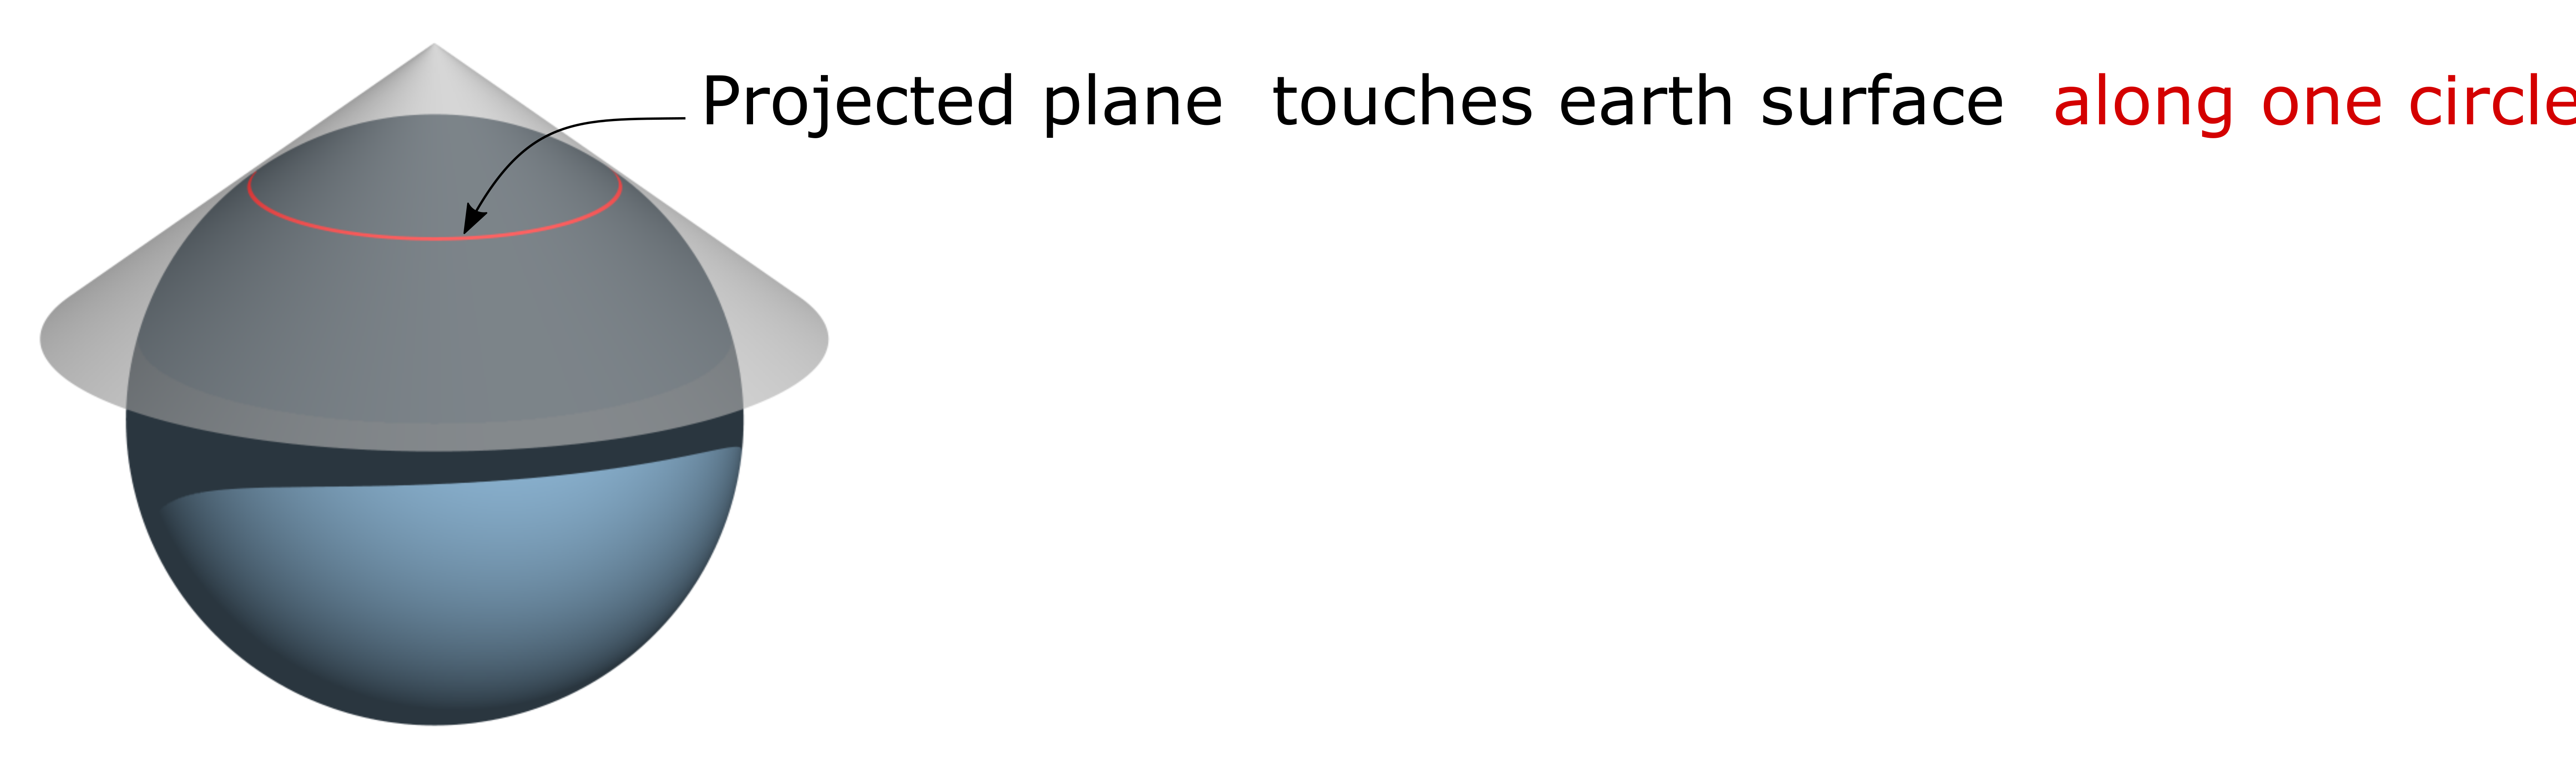
\includegraphics[width=5.98958in,height=\textheight,keepaspectratio]{img/Conical_projection_tangent.png}

}

\caption{\label{fig-tangent3}A tangent conical projection. The
projection surface touches the globe along a single line, where
distortion is minimized.}

\end{figure}%

\begin{figure}[H]

\centering{

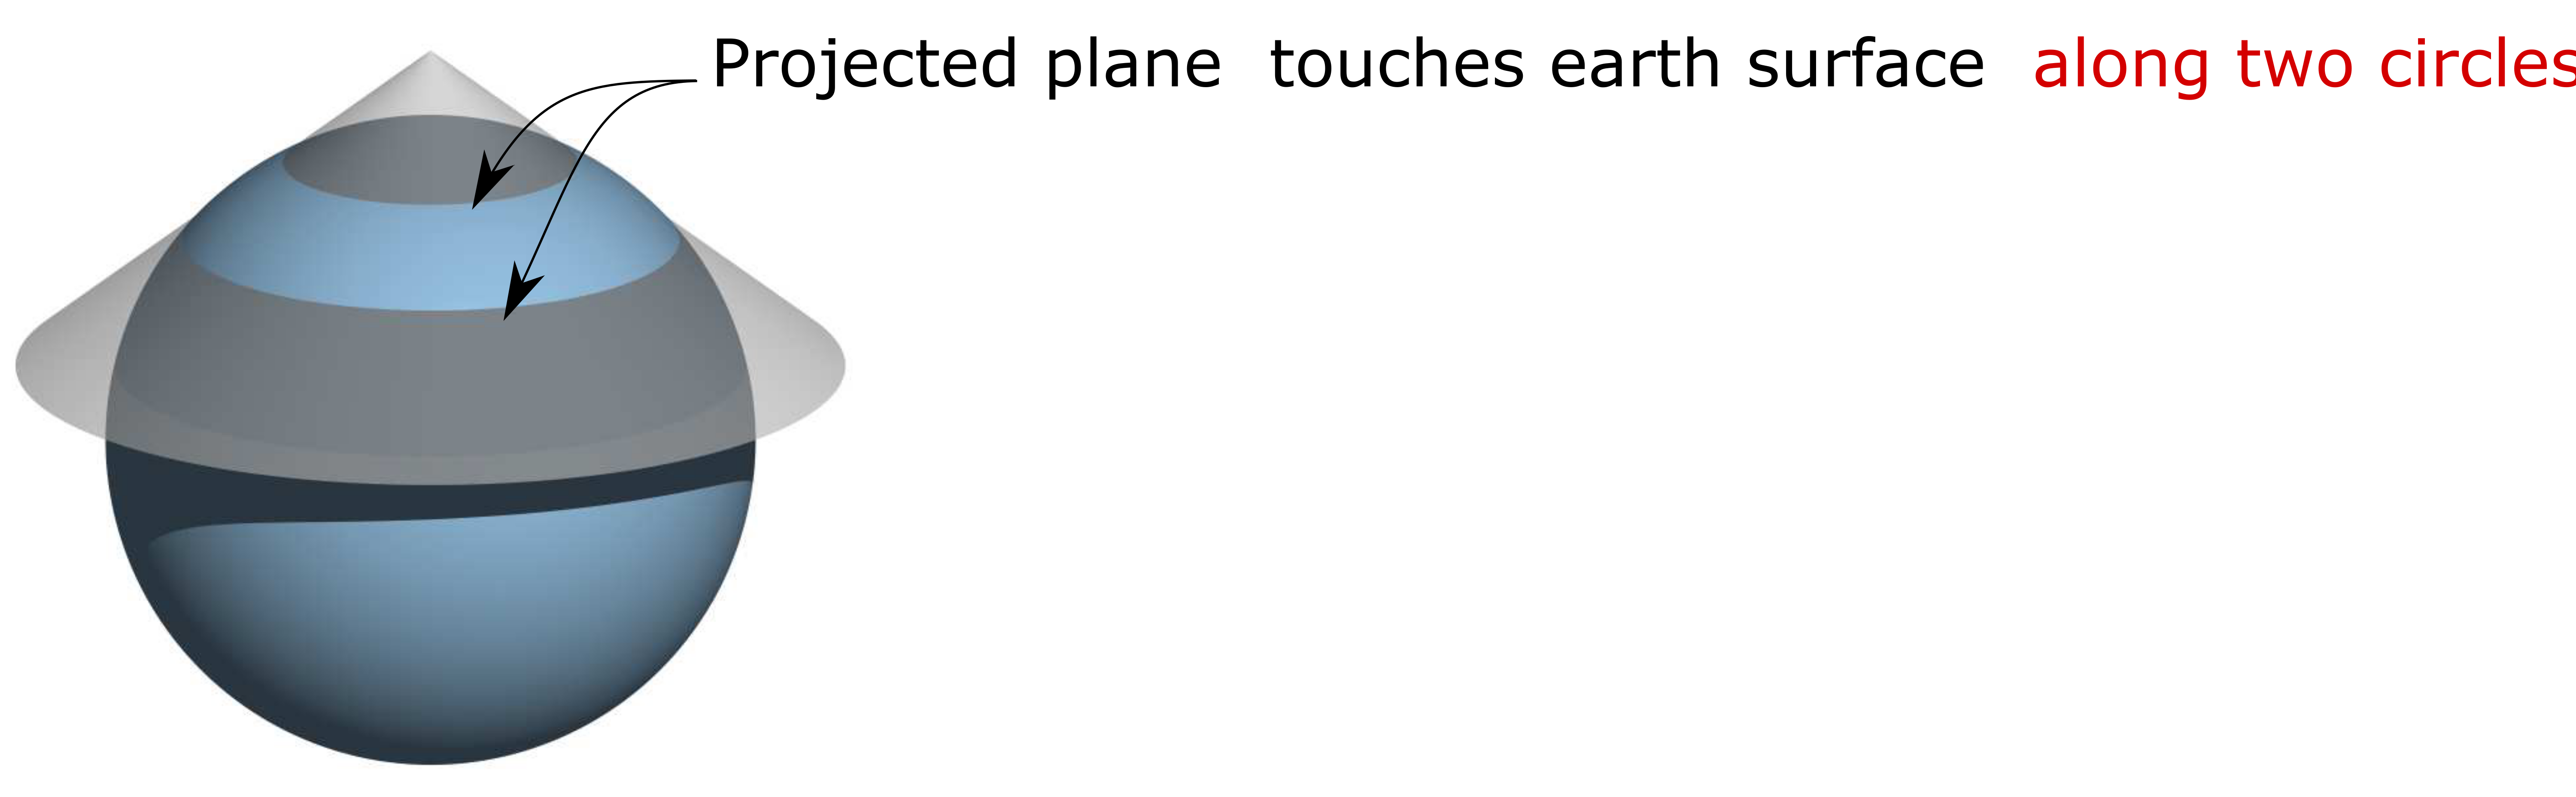
\includegraphics[width=5.98958in,height=\textheight,keepaspectratio]{img/Conical_projection_secant.png}

}

\caption{\label{fig-secant3}A secant conical projection. The projection
surface intersects the globe along two lines, reducing distortion over a
larger region than the tangent case.}

\end{figure}%

Distortion is minimized along the tangent or secant lines and generally
increases with distance from them.

Conical projections are particularly well suited for regions that extend
primarily east-west through the mid-latitudes. Because the lines of
contact can be positioned to span the study region, distortion remains
relatively low throughout much of the map.

For this reason, conical projections are commonly used for mapping the
contiguous United States and much of Europe. Common examples include the
\textbf{Equidistant Conic} projection, which preserves distance, the
\textbf{Albers Equal Area Conic} projection, which preserves area, and
the \textbf{Lambert Conformal Conic} projection, which preserves local
shape.

\begin{figure}[H]

\centering{


\includegraphics[width=5.20833in,height=\textheight,keepaspectratio]{img/Conical_Examples.png}

}

\caption{\label{fig-conical_examples}Examples of three conical
projections: Albers equal area (preserves area), equidistant (preserves
distance) and conformal (preserves shape).}

\end{figure}%

\section{Geodesic Measurements}\label{sec-geodesic}

Projected coordinate systems provide a convenient framework for mapping
and spatial analysis, but they inevitably introduce distortion because
the Earth's curved surface must be represented on a flat plane. As
discussed in the previous sections, the magnitude of this distortion
depends on the projection and the geographic extent of the study area.
For many applications, the resulting errors are small and well within
acceptable limits. However, when measurements span large geographic
areas (such as continents or oceans) projection induced distortions can
become substantial.

One way to reduce these errors is to perform measurements directly on
the ellipsoid rather than on a projected surface. Such measurements are
referred to as \textbf{geodesic measurements}.

A \textbf{geodesic distance} is the shortest distance between two points
on an ellipsoid (or spheroid). Likewise, a \textbf{geodesic area} is an
area measured directly on the ellipsoid. Because these measurements are
computed on the Earth's curved surface, they are independent of any
projected coordinate system. In fact, the Tissot indicatrices introduced
in the previous section were generated using geodesic measurements.

To illustrate the difference between planar and geodesic measurements,
consider the following example. The map below compares the shortest path
between two locations on opposite sides of the Atlantic Ocean. The blue
solid line represents the shortest path measured in a projected
coordinate system (a planar measurement), whereas the red dashed line
represents the geodesic path measured directly on the spheroid.

\begin{figure}[H]

\centering{

\pandocbounded{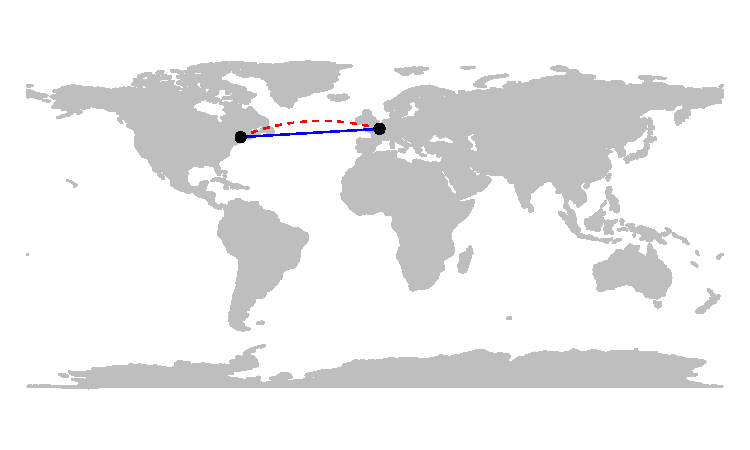
\includegraphics[keepaspectratio]{09_coordinate_systems_files/figure-pdf/fig-dist_comparison-1.pdf}}

}

\caption{\label{fig-dist_comparison}Comparison of planar and geodesic
shortest paths between two locations. The blue line shows the shortest
path measured in a projected coordinate system, whereas the red dashed
line shows the geodesic path measured directly on the spheroid. Although
the geodesic path appears curved on the map, it represents the shortest
route on the Earth's surface.}

\end{figure}%

At first glance, the geodesic path may appear counterintuitive because
it is not represented as a straight line on the projected map. However,
this apparent curvature is a consequence of projecting a curved Earth
onto a flat surface. Although the geodesic path appears curved in the
map view, it represents the shortest route along the Earth's surface. To
better visualize this relationship, we can display both the geodesic and
planar paths on a 3D globe--or on a projection that mimics the Earth as
viewed from space and is centered on the midpoint of the route.

\begin{figure}[H]

\centering{

\pandocbounded{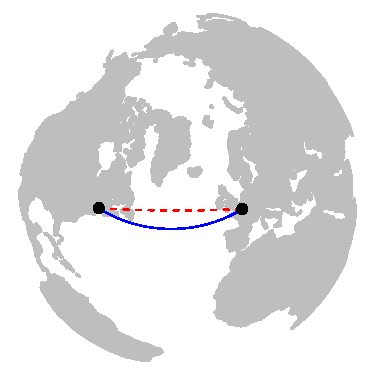
\includegraphics[keepaspectratio]{09_coordinate_systems_files/figure-pdf/fig-geod_vs_plan-1.pdf}}

}

\caption{\label{fig-geod_vs_plan}Geodesic (red dashed) and planar (blue)
paths displayed on a globe-centered view. When viewed on a
representation of the Earth's surface rather than a conventional map
projection, the geodesic path more clearly reveals its role as the
shortest route between the two locations.}

\end{figure}%

So, if geodesic measurements are often more accurate than planar ones,
why not use them for all spatial operations?

In many cases, geodesic methods are perfectly acceptable--and often
preferred. However, they come with a computational cost. Computing
distances and areas on a plane is generally more efficient than
performing the equivalent calculations on an ellipsoid. Whereas planar
measurements often rely on relatively simple geometric formulas,
geodesic calculations typically require more complex mathematical
procedures and, in some cases, iterative approximations. These
additional computations can become significant when processing millions
of vertices or large spatial datasets.

It is also important to note that not all geodesic implementations are
created equal. Different software packages and algorithms make different
tradeoffs between speed and precision. Some methods prioritize
computational efficiency and may sacrifice a small amount of accuracy,
whereas others prioritize accuracy at the expense of processing time.

In R, several packages support geodesic measurements:

\begin{itemize}
\tightlist
\item
  \texttt{geosphere} (based on the authoritative
  \href{https://geographiclib.sourceforge.io/}{GeographicLib}
  libraries),
\item
  \texttt{lwgeom} (an R binding to the
  \href{https://github.com/postgis/postgis/tree/master/liblwgeom}{liblwgeom}
  libraries),
\item
  \texttt{s2} is an implementation of Google's spherical measurement
  library.
\end{itemize}

\section{Summary}\label{summary-7}

This chapter introduced the coordinate systems used to represent
locations on the Earth and examined how different reference systems
influence spatial measurements and mapping.

\begin{itemize}
\item
  A \textbf{spatial reference system} provides the framework used to
  assign coordinates to geographic locations.
\item
  Earth-based coordinate systems can be divided into two broad
  categories: \textbf{Geographic Coordinate Systems (GCS)} and
  \textbf{Projected Coordinate Systems (PCS)}.
\item
  A \textbf{Geographic Coordinate System} uses \textbf{latitude} and
  \textbf{longitude} to identify locations on the Earth's surface. These
  coordinates are angular measurements referenced to the Earth's center.
\item
  The same physical location can have different coordinate values
  depending on the geographic coordinate system used.
\item
  A \textbf{sphere} provides a simple approximation of the Earth, but
  modern geographic coordinate systems typically use an
  \textbf{ellipsoid}, which more accurately reflects the Earth's shape.
\item
  The \textbf{geoid} represents the Earth's gravitational reference
  surface and differs slightly from a smooth ellipsoid because of
  variations in the Earth's gravity field.
\item
  A \textbf{datum} defines how an ellipsoid is aligned relative to the
  Earth. Different datum definitions can produce different coordinate
  values for the same location.
\item
  A \textbf{Geographic Coordinate System} is created by combining an
  ellipsoid with a datum.
\item
  A \textbf{Projected Coordinate System} is created by applying a map
  projection to a Geographic Coordinate System (GCS). Because of this
  dependency, coordinate values may differ even when the same projection
  method is used with different datums.
\item
  Map projections are necessary because latitude and longitude do not
  provide a naturally planar framework for measuring distance, area, and
  direction.
\item
  Every map projection introduces \textbf{distortion}. The four spatial
  properties most commonly affected are \textbf{shape}, \textbf{area},
  \textbf{distance}, and \textbf{direction}.
\item
  Projections that preserve shape are called \textbf{conformal}, those
  that preserve area are \textbf{equal-area}, those that preserve
  distance are \textbf{equidistant}, and those that preserve direction
  are \textbf{azimuthal}.
\item
  \textbf{Tissot indicatrices} provide a useful way to visualize and
  evaluate projection distortion across a map.
\item
  Three common projection families are \textbf{planar},
  \textbf{cylindrical}, and \textbf{conical projections}. Each
  distributes distortion differently and is suited to different mapping
  applications.
\item
  \textbf{Geodesic measurements} compute distances and areas directly on
  the ellipsoid and are independent of the projected coordinate system
  used to display the data. Geodesic methods generally provide more
  accurate measurements over large geographic extents, whereas planar
  measurements are often computationally simpler and sufficiently
  accurate for many local and regional applications.
\item
  Selecting an appropriate coordinate system is an essential step in any
  GIS workflow because coordinate systems influence positional accuracy,
  measurement accuracy, and the interpretation of spatial patterns.
\end{itemize}

\chapter{Map Algebra}\label{map-algebra}

\section{Introduction}\label{introduction-9}

In Chapter 2, raster data were introduced as a spatial data model in
which the study area is represented as a regular grid of cells. Unlike
vector data, where attributes are linked to discrete features such as
points, lines, and polygons, raster datasets assign a value to every
cell in the grid. Because each cell stores a value at a known location,
mathematical and logical operations can be applied systematically across
the entire study area.

This cell-based structure makes raster data particularly well suited for
spatial analysis. For example, we may wish to:

\begin{itemize}
\tightlist
\item
  identify locations with elevations greater than 500 m,
\item
  calculate the average elevation surrounding each cell,
\item
  summarize precipitation for each watershed,
\item
  determine the distance from every location to the nearest road.
\end{itemize}

These types of analyses involve transforming and combining raster values
to generate new spatial information.

One framework for performing such analyses is \textbf{Map Algebra}, a
system of spatial operations developed by \textbf{Dana Tomlin} (Tomlin
1990). Map Algebra treats raster layers as mathematical objects that can
be manipulated using arithmetic, logical, and statistical operations.
The framework organizes raster analysis according to the spatial context
used in the calculation.

Tomlin identified three primary categories of raster operations:

\begin{itemize}
\tightlist
\item
  \textbf{Local operations}, which compute new values using information
  associated with the same location.
\item
  \textbf{Focal operations}, which compute new values using information
  from neighboring locations.
\item
  \textbf{Zonal operations}, which compute new values by summarizing
  information within predefined regions.
\end{itemize}

O'Sullivan and Unwin (O'Sullivan and Unwin 2010) later proposed a fourth
category:

\begin{itemize}
\tightlist
\item
  \textbf{Global operations}, which compute new values using information
  from all locations in the study area.
\end{itemize}

Together, these four categories form the foundation of raster-based
spatial analysis and provide a useful framework for understanding many
GIS tools and modeling workflows.

A useful way to distinguish among map algebra operations is to consider
how much of the raster is involved in computing each output value. At
one extreme, an operation may use only the value stored in a single
cell. At the other extreme, it may draw information from the entire
raster. Between these extremes are operations that use neighboring cells
or predefined regions.

We begin with local operations, the simplest type of map algebra
function, in which the output value is computed using only information
associated with the same location.

\section{Local operations and
functions}\label{local-operations-and-functions}

\textbf{Local operations} are the simplest type of map algebra function.
They compute a new value for each cell using only information associated
with that same location. In other words, the value assigned to an output
cell depends exclusively on the value or values occupying the
corresponding cell location in one or more input rasters.

Because only coincident cell locations are used in the calculation,
local operations do not require information from neighboring cells or
from other parts of the raster. Common local operations include
arithmetic calculations, logical comparisons, and reclassification of
raster values.

For instance, starting with an original raster layer, we might apply a
sequence of operations--first multiplying each cell value by 2, then
adding 1. The result is a new raster in which each cell reflects the
cumulative effect of those operations applied to the corresponding cell
in the original layer. This is an example of a \textbf{unary operation},
where only a single raster is involved in the computation.

The following figure illustrates a local operation in which every cell
value is transformed using the expression
\texttt{output\ =\ (2\ x\ input)\ +\ 1}.

\begin{figure}[H]

\centering{

\pandocbounded{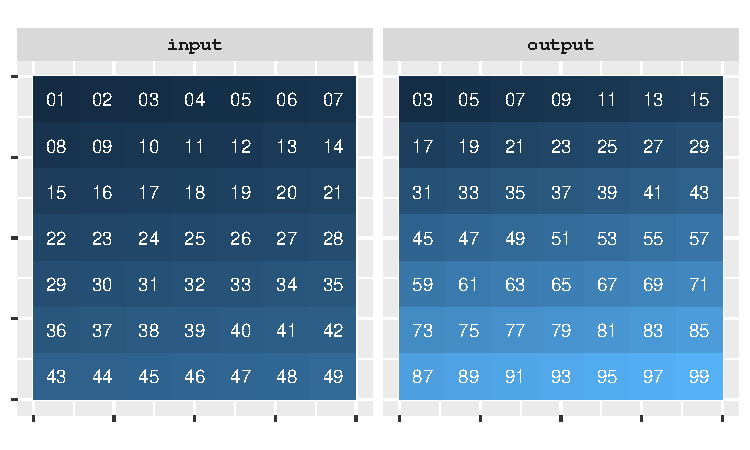
\includegraphics[keepaspectratio]{10_map_algebra_files/figure-pdf/fig-local01-1.pdf}}

}

\caption{\label{fig-local01}Local map algebra operation where each
output cell is computed as \texttt{(2\ ×\ input)\ +\ 1}. The value
assigned to each output cell depends only on the corresponding input
cell.}

\end{figure}%

Local operations can also involve multiple raster layers. In the
previous example, the output values were derived from a single raster
layer. However, local operations can also combine values from two or
more raster layers at the same location.

For example, two rasters can be added together by summing the values of
coincident cells. The resulting raster assigns each output cell the
combined value of the corresponding cells from the input layers. This is
an example of a \textbf{binary operation} because two raster layers
participate in the calculation.

\begin{figure}[H]

\centering{

\pandocbounded{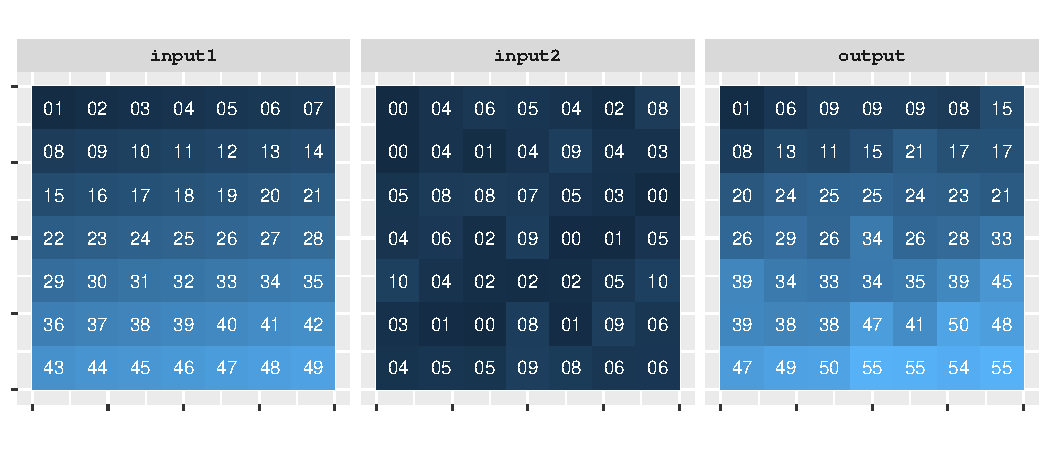
\includegraphics[keepaspectratio]{10_map_algebra_files/figure-pdf/fig-local02-1.pdf}}

}

\caption{\label{fig-local02}Example of a local binary operation where
corresponding cells from two raster layers are added together. Each
output value is computed using only the values stored at the same
location in the input rasters.}

\end{figure}%

Local operations also include \textbf{reclassification}, where a range
of input raster values is assigned a new, common value. Rather than
performing arithmetic on raster values, reclassification groups values
into categories that may be easier to interpret or analyze. Common
applications include converting continuous elevation values into
elevation classes, grouping land suitability scores into categories such
as low, medium, and high suitability, or simplifying a raster prior to
further analysis.

For example, we might reclassify the input raster values as follows:

{\def\LTcaptype{none} % do not increment counter
\begin{longtable}[]{@{}rl@{}}
\toprule\noalign{}
Original values & Reclassified values \\
\midrule\noalign{}
\endhead
\bottomrule\noalign{}
\endlastfoot
1-10 & 10 \\
11-20 & 20 \\
21-30 & 30 \\
31-40 & 40 \\
41-50 & 50 \\
\end{longtable}
}

In this example, every input value between 1 and 10 is assigned an
output value of 10, values between 11 and 20 are assigned 20, and so on.
Because the output value depends only on the value of the corresponding
input cell, reclassification remains a local operation.

\begin{figure}[H]

\centering{

\pandocbounded{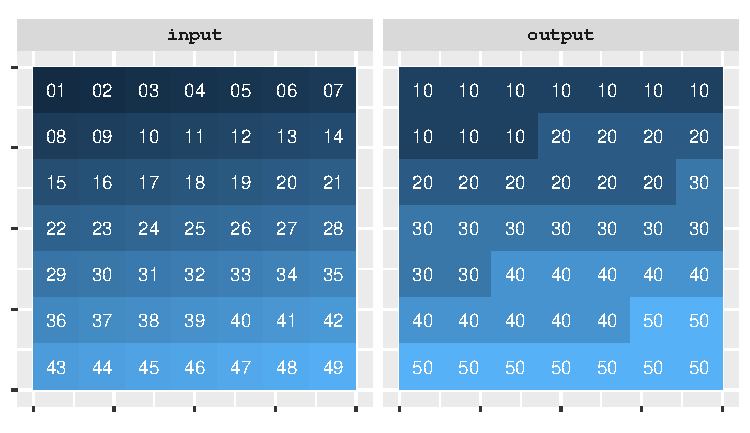
\includegraphics[keepaspectratio]{10_map_algebra_files/figure-pdf/fig-local03-1.pdf}}

}

\caption{\label{fig-local03}Example of a local reclassification
operation. Each output cell is assigned a new value based on the value
range containing the corresponding input cell. Since the transformation
depends only on the input value at the same location, reclassification
is a local operation.}

\end{figure}%

The next category of functions, known as focal operations, expands the
scope of the analysis by incorporating information from neighboring
cells when computing each output value.

\section{Focal operations and
functions}\label{focal-operations-and-functions}

\textbf{Focal operations} differ from local operations in that they
incorporate information from neighboring cells when computing a new
value for each location. Whereas local operations use only the value
associated with the same cell location, focal operations define a
neighborhood around each cell and use information from that neighborhood
in the calculation.

The neighborhood is commonly centered on the cell being evaluated and
may consist of the eight immediately adjacent cells, a larger square or
circular window, or another user-defined shape. The output value
assigned to the center cell therefore depends not only on its own value,
but also on the values of nearby cells.

For example, a focal operation might calculate the average value of all
cells within the neighborhood and assign that average to the center
cell. This approach is often used for \textbf{smoothing} data, reducing
local variability, detecting spatial patterns, and identifying
transitions across a surface.

\begin{figure}[H]

\centering{

\pandocbounded{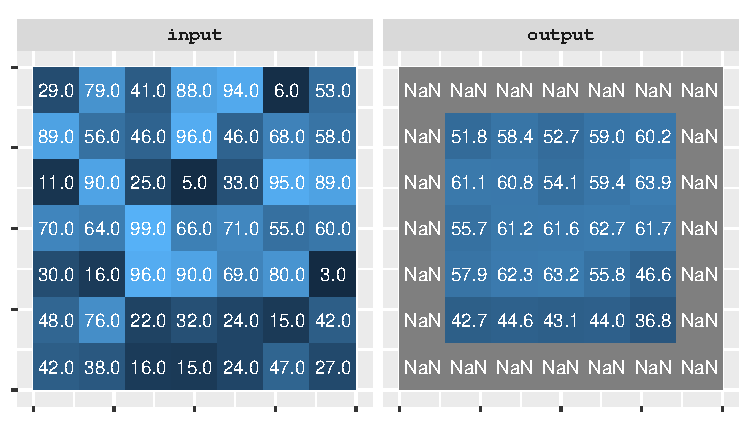
\includegraphics[keepaspectratio]{10_map_algebra_files/figure-pdf/fig-focal01-1.pdf}}

}

\caption{\label{fig-focal01}Example of a focal averaging operation using
a 3×3 neighborhood. Each output cell is assigned the average value of
the corresponding input cell and its surrounding neighbors. Cells along
the raster boundary are assigned NoData values because the full
neighborhood cannot be evaluated.}

\end{figure}%

Notice in the example above that the edge cells in the output raster
have been assigned a value of \texttt{NA} (No Data). This occurs because
the neighborhood around those cells extends beyond the raster boundary,
where no values exist. These boundary-related issues are commonly
referred to as \textbf{edge effects}.

Different GIS applications handle edge effects differently. Some assign
a NoData value whenever the full neighborhood cannot be evaluated, while
others ignore the missing cells and compute the summary statistic using
only the available neighboring values. The latter approach is
demonstrated in the next example.

\begin{figure}[H]

\centering{

\pandocbounded{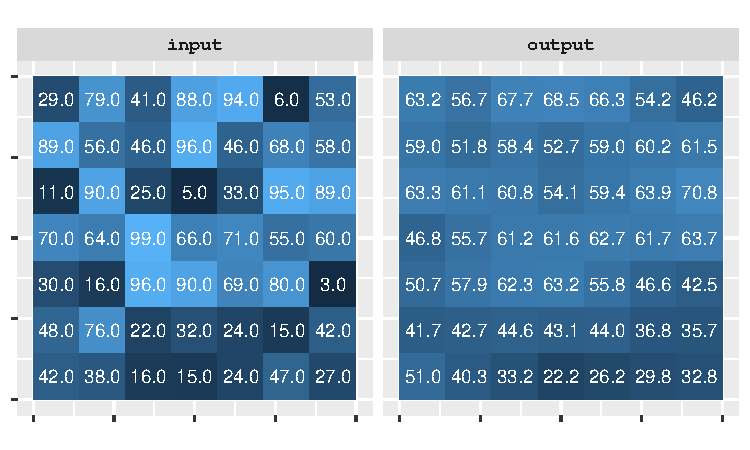
\includegraphics[keepaspectratio]{10_map_algebra_files/figure-pdf/fig-focal02-1.pdf}}

}

\caption{\label{fig-focal02}Focal averaging operation using a 3×3
neighborhood where missing cells beyond the raster boundary are ignored.
Unlike Figure~\ref{fig-focal01}, edge cells receive valid output values
because the average is computed from the available neighboring cells
only.}

\end{figure}%

Focal (or neighborhood) operations require the definition of a window
region, commonly referred to as a \textbf{kernel}. A kernel defines
which neighboring cells contribute to the calculation performed at each
location. In the examples above, a simple 3×3 kernel was used, where
each output value was influenced by the values of cells in the
surrounding neighborhood.

The kernel itself can vary in both size and shape. For example, a focal
operation might use a 3x3 square, or a circular neighborhood defined by
a specified radius. The choice of kernel influences the spatial scale of
the analysis and therefore the resulting output raster.

\begin{figure}[H]

\centering{

\pandocbounded{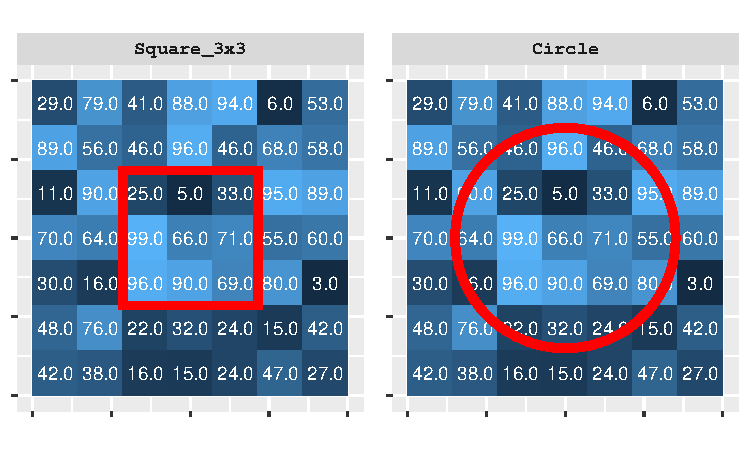
\includegraphics[keepaspectratio]{10_map_algebra_files/figure-pdf/fig-kernels-1.pdf}}

}

\caption{\label{fig-kernels}Examples of kernel shapes used to define
focal neighborhoods. The square kernel includes all cells within a 3 × 3
moving window, whereas the circular kernel includes cells within a
specified radius of the focal cell.}

\end{figure}%

Figure~\ref{fig-kernels} illustrates two common neighborhood
definitions. In practice, focal operations are not limited to selecting
a neighborhood shape; they can also specify which cells within that
neighborhood participate in the calculation. For example, a 3×3 square
kernel may include all nine cells or exclude the center cell, depending
on the analytical objective.

The following example uses a 3×3 square kernel in which the center cell
is \emph{excluded}. As a result, each output value is computed from the
eight neighboring cells surrounding the focal location rather than from
the focal cell itself.

\begin{figure}[H]

\centering{

\pandocbounded{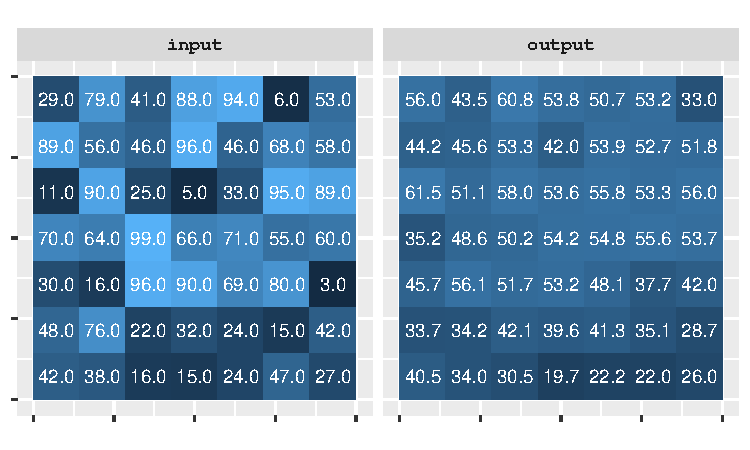
\includegraphics[keepaspectratio]{10_map_algebra_files/figure-pdf/fig-focal03-1.pdf}}

}

\caption{\label{fig-focal03}Focal averaging operation using a 3×3 kernel
with the center cell excluded. Each output value is computed from the
eight neighboring cells surrounding the target location.}

\end{figure}%

In addition to defining the shape and size of the neighborhood, a kernel
can also specify how much influence each neighboring cell has on the
output value. This influence is expressed through a set of
\textbf{weights} assigned to the cells within the kernel.

For example, in a 3×3 neighborhood used for focal averaging, each cell
might contribute an equal weight of 1/9 to the final value. Such a
kernel treats all neighboring cells as equally important. However,
weights can also be assigned unequally to emphasize some cells more than
others. These weighted neighborhoods are often defined using
\textbf{kernel functions}.

One commonly used kernel function is the \textbf{Gaussian} kernel, which
assigns greater weight to cells near the center of the neighborhood and
progressively smaller weights to cells farther away. As a result, nearby
cells exert a stronger influence on the output value than distant cells.

The following example applies a Gaussian kernel to the same raster used
in the previous examples.

\begin{figure}[H]

\centering{

\pandocbounded{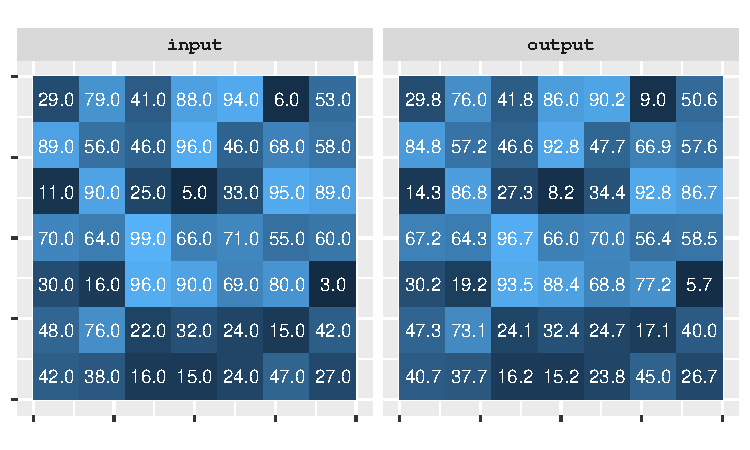
\includegraphics[keepaspectratio]{10_map_algebra_files/figure-pdf/fig-focal04-1.pdf}}

}

\caption{\label{fig-focal04}Focal averaging operation using a Gaussian
kernel. Cells closest to the center of the neighborhood receive the
greatest weight, causing nearby values to exert more influence on the
output than distant values.}

\end{figure}%

Thus far, focal operations have summarized values within neighborhoods
centered on individual cells. In many applications, however, we are
interested in summarizing values across larger predefined regions such
as watersheds, counties, or management units. These are the focus of
zonal operations.

\section{Zonal operations and
functions}\label{zonal-operations-and-functions}

\textbf{Zonal operations} differ from local and focal operations in that
they summarize values across predefined regions rather than individual
cells or neighborhoods. Whereas focal operations define a neighborhood
around every cell, zonal operations define larger regions, called
\textbf{zones}, that may contain many cells.

A zone is typically derived from a separate raster or polygon layer and
represents a meaningful geographic region such as a watershed, county,
land parcel, or landcover class. All cells belonging to the same zone
are treated as a single analytical unit.

Zonal operations compute a summary statistic for each zone using the
values from another raster layer. Common summary statistics include the
mean, sum, minimum, maximum, and standard deviation.

In the following example, raster cell values are aggregated into three
zones whose boundaries are delineated by red polygons. Each output zone
is assigned the average value of the cells contained within that zone.

\begin{figure}[H]

\centering{

\pandocbounded{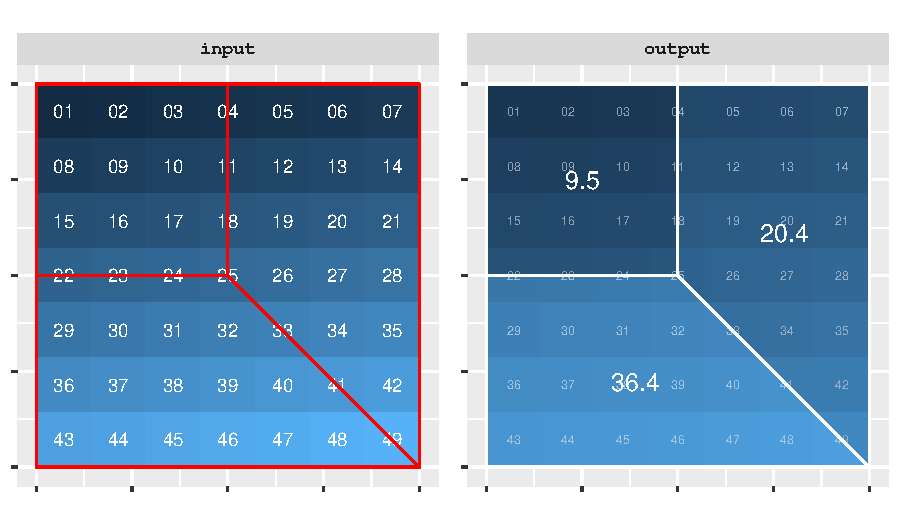
\includegraphics[keepaspectratio]{10_map_algebra_files/figure-pdf/fig-zonal01-1.pdf}}

}

\caption{\label{fig-zonal01}Example of a zonal operation in which raster
values are averaged within three predefined zones. All cells belonging
to the same zone contribute to a single summary value, which is then
assigned to the entire zone.}

\end{figure}%

Although zonal operations can generate new spatial layers, the output is
often tabular rather than spatial. In many GIS workflows, the goal is to
summarize a raster variable for a set of spatial regions rather than
create a new map. For example, a zonal operation might be used to
calculate the average elevation within each state, the total population
within each watershed, or the percentage of each county covered by
water. The resulting output is typically a table in which each zone is
associated with one or more summary statistics. Thus, zonal operations
serve as an important bridge between raster and vector data by
summarizing raster values for meaningful geographic regions.

Local, focal, and zonal operations all compute output values using
information drawn from a limited spatial context. In contrast, some
raster operations require information from the entire study area when
calculating output values. These are known as global operations.

\section{Global operations and
functions}\label{global-operations-and-functions}

\textbf{Global operations} and functions may use some or all input cells
when computing the value of each output cell. Unlike local, focal, and
zonal operations, which rely on information from a limited spatial
context, global operations draw information from potentially the entire
study area.

A common example is the \textbf{Euclidean Distance} tool, which
calculates the shortest straight-line distance between each cell and a
specified source or destination. In the example below, a new raster
assigns to each cell the distance to the nearest cell with a value of
1-note that only two such cells exist in the input raster.

\begin{figure}[H]

\centering{

\pandocbounded{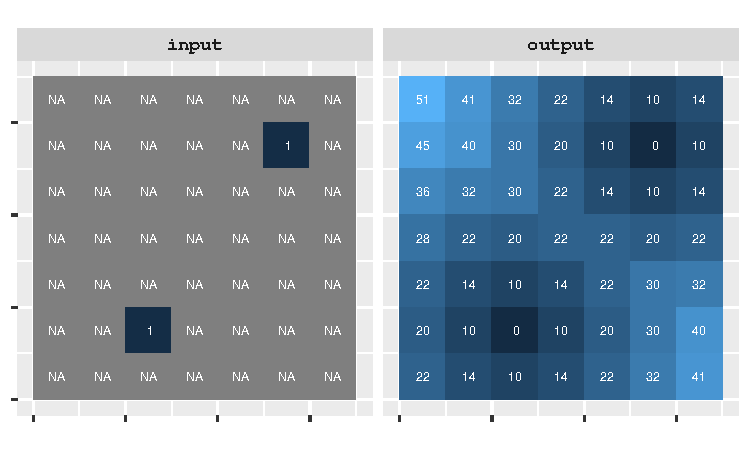
\includegraphics[keepaspectratio]{10_map_algebra_files/figure-pdf/fig-global01-1.pdf}}

}

\caption{\label{fig-global01}Example of a global operation using
Euclidean distance. Each output cell is assigned the shortest
straight-line distance to the nearest source cell (value = 1) in the
input raster. Each cell's dimension is 10 by 10 units. Unlike local,
focal, and zonal operations, the calculation may require information
from locations across the entire raster.}

\end{figure}%

Euclidean distance is only one example of a global operation. Other
global functions may compute summary statistics for an entire raster,
identify least-cost paths across a landscape, or evaluate measures of
spatial dependence. What these approaches have in common is that the
calculation potentially depends on information drawn from all locations
in the study area.

\section{Operators and functions}\label{operators-and-functions}

Thus far, we have focused on the spatial context of raster
operations---whether calculations are performed at individual cells,
within neighborhoods, across zones, or using information from an entire
raster. Regardless of the spatial context, raster calculations are
ultimately built from a relatively small set of operators and functions.

These operators and functions can be grouped into three broad
categories:

\begin{itemize}
\tightlist
\item
  \textbf{Mathematical operators and functions}, which perform
  arithmetic calculations on raster values.
\item
  \textbf{Logical comparison operators}, which evaluate whether
  specified conditions are true or false.
\item
  \textbf{Boolean operators}, which combine multiple logical conditions
  into more complex expressions.
\end{itemize}

These building blocks can be used individually or combined to create
more sophisticated map algebra expressions.

\subsection{Mathematical operators and
functions}\label{mathematical-operators-and-functions}

Many map algebra operations rely on familiar \textbf{mathematical
expressions}. In fact, several mathematical operators have already been
introduced in the local operation examples, including multiplication and
addition. These operators manipulate raster values using arithmetic
rules similar to those used in spreadsheets and programming languages.

Common mathematical operators include addition, subtraction,
multiplication, division, and the modulo (or modulus) operator, which
returns the remainder of a division. Mathematical functions can also be
applied to raster values. Examples include square-root, logarithmic,
trigonometric, and exponential functions.

The following table lists a few commonly used operators and functions
together with their ArcGIS and R syntax.

{\def\LTcaptype{none} % do not increment counter
\begin{longtable}[]{@{}
  >{\raggedright\arraybackslash}p{(\linewidth - 6\tabcolsep) * \real{0.2941}}
  >{\raggedright\arraybackslash}p{(\linewidth - 6\tabcolsep) * \real{0.2353}}
  >{\raggedright\arraybackslash}p{(\linewidth - 6\tabcolsep) * \real{0.2353}}
  >{\raggedright\arraybackslash}p{(\linewidth - 6\tabcolsep) * \real{0.2353}}@{}}
\toprule\noalign{}
\begin{minipage}[b]{\linewidth}\raggedright
Operation
\end{minipage} & \begin{minipage}[b]{\linewidth}\raggedright
ArcGIS Syntax
\end{minipage} & \begin{minipage}[b]{\linewidth}\raggedright
R Syntax
\end{minipage} & \begin{minipage}[b]{\linewidth}\raggedright
Example
\end{minipage} \\
\midrule\noalign{}
\endhead
\bottomrule\noalign{}
\endlastfoot
Addition & \texttt{+} & \texttt{+} & \texttt{input1\ +\ input2} \\
Subtraction & \texttt{-} & \texttt{-} & \texttt{input1\ -\ input2} \\
Multiplication & \texttt{*} & \texttt{*} & \texttt{input1\ *\ input2} \\
Division & \texttt{/} & \texttt{/} & \texttt{input1\ /\ input2} \\
Modulo & \texttt{Mod()} & \texttt{\%\%} & \texttt{Mod(input1,\ 100)},
\texttt{input1\ \%\%\ 10} \\
Square root & \texttt{SquareRoot()} & \texttt{sqrt()} &
\texttt{SquareRoot(input1)}, \texttt{sqrt(input1)} \\
\end{longtable}
}

Mathematical operators are frequently used to transform raster values,
combine multiple raster layers, and compute suitability or risk indices
from several input variables.

The operators and functions introduced thus far generate new numeric
raster values. In many GIS applications, however, we are interested in
identifying locations that satisfy specific criteria rather than
computing new numeric quantities. Such operations rely on logical
comparison operators.

\subsection{Logical comparison}\label{logical-comparison}

Unlike mathematical operators, which generate new numeric values,
\textbf{logical comparison operators} evaluate whether a condition is
true or false. The result is typically stored as a value of \texttt{1}
if the condition is true and \texttt{0} if the condition is false.

Logical comparison operators include \emph{greater than}, \emph{less
than}, \emph{equal}, and \emph{not equal}.

{\def\LTcaptype{none} % do not increment counter
\begin{longtable}[]{@{}ll@{}}
\toprule\noalign{}
Logical comparison & Syntax \\
\midrule\noalign{}
\endhead
\bottomrule\noalign{}
\endlastfoot
Greater than & \texttt{\textgreater{}} \\
Less than & \texttt{\textless{}} \\
Equal & \texttt{==} \\
Not equal & \texttt{!=} \\
\end{longtable}
}

For example, the following figure compares two rasters on a cell-by-cell
basis using the expression \texttt{input1\ \textgreater{}\ input2}.
Cells where the condition is true are assigned a value of \texttt{1},
whereas cells where the condition is false are assigned a value of
\texttt{0}.

\begin{figure}[H]

\centering{

\pandocbounded{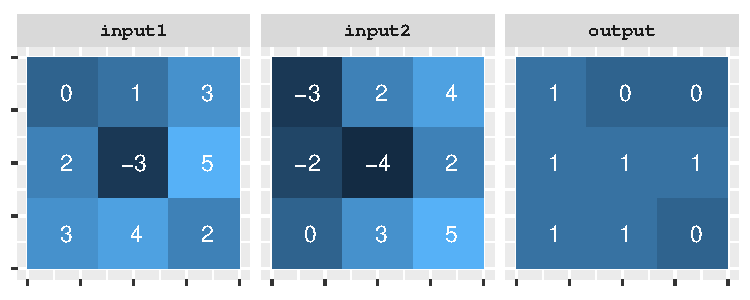
\includegraphics[keepaspectratio]{10_map_algebra_files/figure-pdf/fig-logical01-1.pdf}}

}

\caption{\label{fig-logical01}Output of the logical comparison
\texttt{input1} \textgreater{} \texttt{input2}. Each output cell is
assigned a value of \texttt{1} when the corresponding cell in
\texttt{input1} is greater than the corresponding cell in
\texttt{input2}, and a value of \texttt{0} otherwise.}

\end{figure}%

Logical comparison operations are commonly used to identify locations
that satisfy specified criteria. For example, they can be used to select
areas with elevations greater than 500 m, slopes steeper than 15°, or
distances less than 100 m from a road. The resulting binary raster can
then be used in subsequent map algebra operations.

When assessing whether two cells are equal, some programming
environments such as R and ArcGIS's \emph{Raster Calculator} require the
use of the \emph{double equality} syntax, \texttt{==}, as in
\texttt{input1\ ==\ input2}. In these programming environments, the
single equality syntax is usually interpreted as an \emph{assignment
operator} so \texttt{input1\ =\ input2} would instruct the computer to
assign the cell values in \texttt{input2} to \texttt{input1} (which is
not what we want to do here).

Some applications make use of special functions to test a condition. For
example, ArcGIS has a function called
\texttt{Con(condition,\ out1,\ out2)} which assigns the value
\texttt{out1} if the condition is met and a value of \texttt{out2} if
it's not. For example, ArcGIS's raster calculator expression

\begin{verbatim}
Con( input1 > input2, 1, 0)
\end{verbatim}

outputs a value of \texttt{1} if \texttt{input1} is greater than
\texttt{input2} and \texttt{0} if not. It generates the same output as
the one shown in the above figure. In many programming environments,
including ArcGIS and R, \texttt{TRUE} and \texttt{FALSE} can be
represented numerically as \texttt{1} and \texttt{0}, respectively. As a
result, the expression \texttt{input1\ \textgreater{}\ input2} often
produces the same output as
\texttt{Con(input1\ \textgreater{}\ input2,\ 1,\ 0)}.

The comparison operators introduced in this section evaluate a single
condition. In many GIS applications, however, we are interested in
locations that must satisfy multiple conditions simultaneously. Such
expressions are constructed using Boolean operators.

\subsection{Boolean (or Logical)
operators}\label{boolean-or-logical-operators}

Comparison operators evaluate a single condition and return a value of
\texttt{TRUE} or \texttt{FALSE} (often represented as \texttt{1} and
\texttt{0}). In many GIS applications, however, a single condition is
not sufficient. We may wish to identify locations that satisfy multiple
criteria simultaneously. For example, a suitability analysis might seek
locations that are both within 100 m of a road and on slopes less than
15°.

\textbf{Boolean operators} provide a way to combine multiple logical
conditions into a single expression. The three Boolean operators are
\textbf{AND}, \textbf{OR} and \textbf{NOT}.

{\def\LTcaptype{none} % do not increment counter
\begin{longtable}[]{@{}llll@{}}
\toprule\noalign{}
Boolean & ArcGIS & R & Example \\
\midrule\noalign{}
\endhead
\bottomrule\noalign{}
\endlastfoot
AND & \& & \& & \texttt{input1\ \&\ input2} \\
OR & \texttt{\textbar{}} & \texttt{\textbar{}} &
\texttt{input1\ \textbar{}\ input2} \\
NOT & \texttt{\textasciitilde{}} & \texttt{!} &
\texttt{\textasciitilde{}input2}, \texttt{!\ input2} \\
\end{longtable}
}

In many programming environments, any non-zero value is treated as
\texttt{TRUE}, whereas a value of \texttt{0} is treated as
\texttt{FALSE}. The Boolean operators act on these logical states rather
than on the original raster values.

For example:

\begin{itemize}
\tightlist
\item
  \textbf{AND} returns \texttt{TRUE} only if both conditions are true.
\item
  \textbf{OR} returns \texttt{TRUE} if at least one condition is true.
\item
  \textbf{NOT} reverses a logical condition, changing \texttt{TRUE} to
  \texttt{FALSE} and \texttt{FALSE} to \texttt{TRUE}.
\end{itemize}

The following example demonstrates the \textbf{AND} operator applied to
two rasters. Because non-zero values are treated as \texttt{TRUE}, a
cell in the output raster is assigned a value of \texttt{1} only when
both corresponding input cells are non-zero.

\begin{figure}[H]

\centering{

\pandocbounded{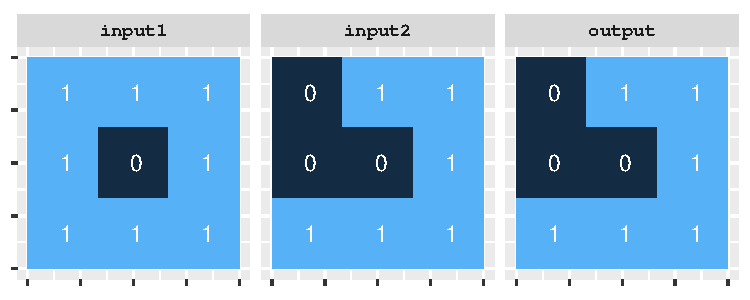
\includegraphics[keepaspectratio]{10_map_algebra_files/figure-pdf/fig-boolean01-1.pdf}}

}

\caption{\label{fig-boolean01}Output of the Boolean operation
\texttt{input1\ AND\ input2}. Because all non-zero values are
interpreted as \texttt{TRUE}, an output cell is assigned a value of
\texttt{1} only when both corresponding input cells are non-zero.
Otherwise, the output value is \texttt{0}.}

\end{figure}%

The \textbf{AND} operator is often used to identify locations that
satisfy multiple criteria simultaneously. Two other commonly used
Boolean operators are \textbf{OR} and \textbf{NOT}. The \textbf{OR}
operator returns \texttt{TRUE} if at least one of the specified
conditions is true, whereas the \textbf{NOT} operator reverses a logical
state, converting \texttt{TRUE} values to \texttt{FALSE} and
\texttt{FALSE} values to \texttt{TRUE}.

\begin{figure}[H]

\centering{

\pandocbounded{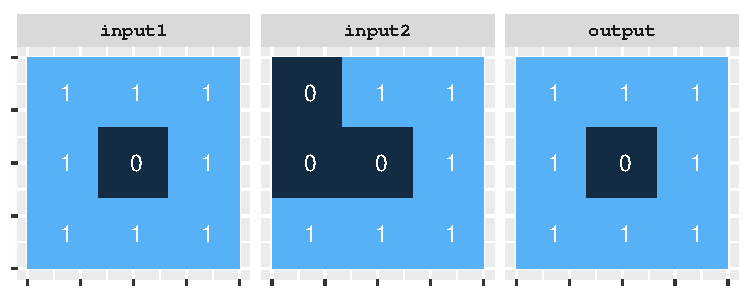
\includegraphics[keepaspectratio]{10_map_algebra_files/figure-pdf/fig-boolean02-1.pdf}}

}

\caption{\label{fig-boolean02}Output of the Boolean operation
\texttt{input1\ OR\ input2}. Because all non-zero values are interpreted
as \texttt{TRUE}, an output cell is assigned a value of \texttt{1}
whenever at least one of the corresponding input cells is non-zero.
Otherwise, the output value is \texttt{0}.}

\end{figure}%

The \textbf{NOT} operator is particularly useful when excluding
locations from an analysis. For example, if a raster uses non-zero
values to indicate suitable locations and zeros to indicate unsuitable
locations, applying the NOT operator reverses this classification. The
following example demonstrates the effect of applying the NOT operator
to a raster layer.

\begin{figure}[H]

\centering{

\pandocbounded{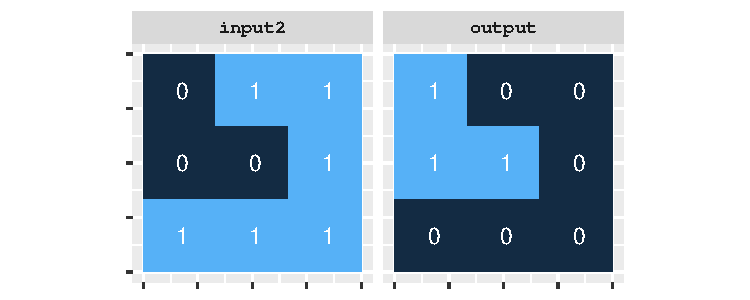
\includegraphics[keepaspectratio]{10_map_algebra_files/figure-pdf/fig-boolean03-1.pdf}}

}

\caption{\label{fig-boolean03}Output of the Boolean operation
\texttt{NOT\ input2}. Cells with a value of \texttt{0} (FALSE) in the
input raster are assigned a value of \texttt{1} (TRUE) in the output
raster, whereas all non-zero values (TRUE) are converted to \texttt{0}
(FALSE).}

\end{figure}%

\subsection{Combining operations}\label{combining-operations}

In practice, raster analyses rarely rely on a single comparison or
Boolean operation. More often, multiple conditions are combined to
identify locations that meet a specific set of criteria. This approach
is common in suitability analysis, where candidate locations must
satisfy several environmental, geographic, or regulatory requirements
simultaneously.

Complex map algebra expressions are typically constructed by first
evaluating individual conditions using comparison operators. Each
comparison produces a raster of \texttt{TRUE} and \texttt{FALSE} values
(often represented as \texttt{1} and \texttt{0}). These logical rasters
can then be combined using Boolean operators such as \textbf{AND},
\textbf{OR}, and \textbf{NOT}.

For example, suppose we wish to identify locations where raster values
in \texttt{input1} are greater than 0 but less than 4, and where
corresponding values in \texttt{input2} are also greater than 0. This
expression can be written as
\texttt{((input1\ \textgreater{}\ 0)\ \&\ (input1\ \textless{}\ 4))\ \&\ (input2\ \textgreater{}\ 0)}.

The following figure illustrates the result of applying this combined
expression to the two raster layers.

\begin{figure}[H]

\centering{

\pandocbounded{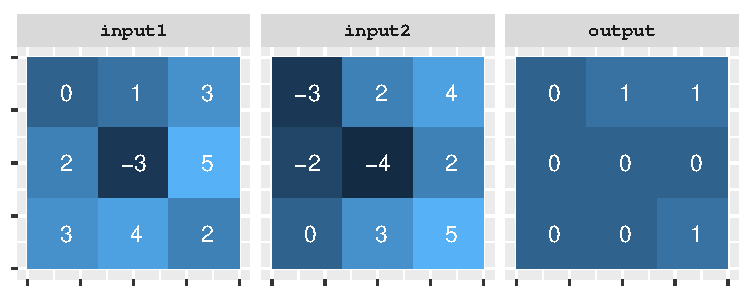
\includegraphics[keepaspectratio]{10_map_algebra_files/figure-pdf/fig-combining01-1.pdf}}

}

\caption{\label{fig-combining01}Output of the operation
((\texttt{input1}\textgreater{}\texttt{0}) \&
(\texttt{input1}\textless{}\texttt{4})) \&
(\texttt{input2}\textgreater{}\texttt{0}). A value of 1 in the output
raster indicates that the condition is true and a value of 0 indicates
that the condition is false.}

\end{figure}%

Expressions such as this form the foundation of many raster suitability
analyses. For example, suppose we are interested in identifying
locations suitable for a new solar farm. We might require that:

\begin{itemize}
\tightlist
\item
  slope be less than 10°,
\item
  distance to roads be less than 500 m, and
\item
  land cover not be classified as wetlands.
\end{itemize}

Each criterion can be evaluated separately using comparison operators.
The resulting logical rasters can then be combined using Boolean
operators to identify locations that satisfy all requirements
simultaneously.

In practice, many raster suitability analyses assign scores to criteria
and combine them using mathematical operators in addition to Boolean
constraints. For example, slope, solar exposure, and distance to
infrastructure might each be assigned suitability scores that are summed
or weighted to produce an overall suitability index, while Boolean
expressions are used to exclude areas that fail to meet minimum
requirements.

\section{Summary}\label{summary-8}

This chapter introduced \textbf{Map Algebra}, a framework for analyzing
raster data using mathematical and logical operations.

\begin{itemize}
\item
  Raster data are well suited to map algebra because every cell stores a
  value at a known location.
\item
  Map algebra operations can be grouped into four categories:

  \begin{itemize}
  \tightlist
  \item
    \textbf{Local}: uses information from the same cell.
  \item
    \textbf{Focal}: uses information from neighboring cells.
  \item
    \textbf{Zonal}: summarizes values within predefined regions.
  \item
    \textbf{Global}: uses information from part or all of the raster.
  \end{itemize}
\item
  Raster calculations can be built using \textbf{mathematical},
  \textbf{logical comparison}, and \textbf{Boolean} operators.
\item
  Comparison operators evaluate conditions and return
  \textbf{TRUE/FALSE} (or \textbf{1/0}) values.
\item
  Boolean operators such as \textbf{AND}, \textbf{OR}, and \textbf{NOT}
  combine multiple conditions into a single expression.
\item
  Map algebra provides the foundation for many raster-based analyses
  including suitability modeling, terrain analysis, and environmental
  modeling.
\end{itemize}

\part{Spatial Analysis}

\chapter{Analyzing Spatial Patterns}\label{chp11_0}

\section{Introduction}\label{introduction-10}

Spatial data are pervasive in daily life and scientific research, from
disease outbreaks to precipitation distribution. We often look at these
maps and intuitively recognize patterns: clusters of events, gradients
across space, or areas of unusual activity. But how do we move from
visual impressions to statistical analysis?

This chapter lays the conceptual foundation for spatial statistical
analysis by introducing spatial processes, which generate the observed
patterns we analyze. We begin by defining what it means to quantify a
spatial pattern, and then explore how spatial processes can be
characterized through two key lenses: \textbf{first-order effects},
which describe broad spatial trends, and \textbf{second-order effects},
which capture local interactions or dependencies.

Understanding this distinction is essential for interpreting spatial
patterns. It helps us answer questions like: Is this cluster of events
meaningful, or could it have occurred by chance? Are nearby observations
influencing each other, or is there an underlying gradient driving the
pattern?

\section{From Maps to Models: Defining Spatial Patterns
Statistically}\label{from-maps-to-models-defining-spatial-patterns-statistically}

Spatial processes may include both deterministic and stochastic
components. The deterministic part reflects systematic variation---such
as a spatial trend or the influence of known covariates---while the
stochastic part captures random variation or uncertainty, including
spatial dependence. Most statistical techniques in spatial analysis
(including those covered in subsequent chapters) combine these elements,
allowing us to describe both the predictable and unpredictable aspects
of spatial patterns.

To analyze these patterns, we need a statistical baseline--a null model
that represents the absence of spatial structure. The most common is
\textbf{Complete Spatial Randomness (CSR)}, which assumes:

\begin{itemize}
\tightlist
\item
  \textbf{No First-Order Effects:} Every location has an equal
  probability of hosting an event, meaning the event intensity or
  density is constant across the study area.
\item
  \textbf{No Second-Order Effects:} The location of one event is
  independent of the location of another, implying \textbf{no spatial
  interaction} or clustering/dispersion among events.
\end{itemize}

For \textbf{point patterns} this is characterized as a
\textbf{homogeneous Poisson process} where events occur independently
and are uniformly distributed across the study region. For
\textbf{attribute data} (such as values measured at fixed locations or
aggregated to areas) the analogous null hypothesis often assumes that
observed spatial variation is purely random.

CSR provides a reference against which observed patterns can be
compared. Deviations from these benchmarks of \emph{no spatial
structure} suggest the presence of non-random spatial structure, which
can manifest as either large-scale variation (first-order process) or
local spatial dependence (second-order process). It is important to note
that \textbf{distinguishing between these first- and second-order
effects from a single observed pattern can be challenging}.

Many spatial methods also assume some form of stationarity, meaning that
the statistical properties of the process do not vary across space.
Violations of this assumption often manifest as first-order effects.

\subsection{First-Order Effects: Spatial Trend and
Intensity}\label{first-order-effects-spatial-trend-and-intensity}

\textbf{First-order effects} describe the \textbf{large-scale variation}
or \textbf{spatial trend} of a phenomenon across space. For
\textbf{point patterns}, this involves how the event intensity (the
average rate or expected number of events) varies. For
\textbf{attribute} data (such as continuous fields or values aggregated
to areas), it refers to how the mean or expected value of the attribute
changes systematically across the study region. These effects reflect
broad, underlying factors that influence the spatial distribution of the
observed phenomena

Examples:

\begin{itemize}
\tightlist
\item
  Tree density increasing with elevation or soil type.
\item
  Crime rates higher in urban centers due to population density.
\item
  Rainfall decreasing as one moves westward.
\end{itemize}

If not accounted for, strong first-order trends can create the illusion
of clustering or dispersion. This highlights a crucial challenge in
spatial analysis: it can be difficult to distinguish between first-order
variation and true inter-point interaction (second-order effects) from a
single observed pattern. For instance, a gradient in tree density might
appear as a cluster when viewed on a map, even if no local interaction
exists.

\subsection{Second-Order Effects: Interaction and
Autocorrelation}\label{second-order-effects-interaction-and-autocorrelation}

\textbf{Second-order effects} describe local dependencies--how the
presence or value of one observation influences others nearby.

Examples:

\begin{itemize}
\tightlist
\item
  Trees clustering due to seed dispersal.
\item
  High crime rates spreading to adjacent neighborhoods due to local
  dynamics.
\end{itemize}

For point data, these are often called \textbf{interactions} between
events, while for continuous field data, they are referred to as
\textbf{spatial autocorrelation}. Analyzing second-order properties
typically involves assessing patterns of interaction \textbf{beyond any
underlying spatial trend or varying intensity}.

\begin{figure}[H]

\centering{


\includegraphics[width=6.25in,height=\textheight,keepaspectratio]{img/1st_2nd_order_property.png}

}

\caption{\label{fig-1st_2nd_effects}Conceptual illustration of
first-order and second-order effects. First-order effects arise from
spatial variation in environmental or socioeconomic factors that cause
intensity or attribute values to vary across space. Second-order effects
arise from interactions among observations themselves, producing
clustering, dispersion, or spatial autocorrelation. Much of the
remainder of this part of the book is organized around distinguishing
and modeling these two forms of spatial structure.}

\end{figure}%

\section{Why Distinguishing These Effects
Matters}\label{why-distinguishing-these-effects-matters}

First-order and second-order effects offer complementary insights into
spatial patterns. An observed cluster might be due to a spatial trend
(first-order), local interaction (second-order), or both. However,
\textbf{it is often difficult to distinguish these effects in practice
from a single observed pattern}. Failing to distinguish between these
can lead to incorrect conclusions about the underlying process, a common
pitfall in spatial analysis. From a single realization, it is
mathematically impossible to distinguish between a process of
independent events generated under a heterogeneous intensity and one of
dependent events generated under homogeneous intensity.

In practice, realistic null hypotheses often account for first-order
effects when testing for second-order ones. For example, we might use a
\textbf{heterogeneous Poisson process} to model varying intensity across
space. This model assumes that event intensity or the likelihood of
observing a point changes spatially due to external factors, but
critically, it still assumes that events occur independently of each
other. Thus, it serves as a baseline to test for clustering or
interaction beyond any underlying spatial trend.

In many spatial analyses, first-order effects are modeled first, and
second-order effects are then examined in the residuals that remain
after the first-order structure has been removed.

\section{Spatial Data Types and Applicability of First- and Second-Order
Effects}\label{spatial-data-types-and-applicability-of-first--and-second-order-effects}

We learned in \hyperref[object-vs.-field]{chapter 2} that spatial data
can be broadly categorized into two types: \textbf{object-based}, which
treat the world as discrete entities located in space (e.g., points for
crime locations or tree positions, or polygons for administrative
boundaries), and \textbf{field-based}, which represent continuous
phenomena measured across space (such as temperature, elevation, or
precipitation). These distinct representations influence the methods
used to analyze spatial patterns.

Regardless of the data type, the concepts of first-order and
second-order effects apply. For point data, first-order effects describe
variations in \textbf{event intensity} across space, while second-order
effects capture \textbf{interactions} between events. For continuous
fields, first-order effects are often modeled using \textbf{trend
surfaces} and \textbf{interpolation methods}, while second-order effects
are commonly examined through measures of \textbf{spatial
autocorrelation}.

Understanding the nature of the data helps determine the appropriate
analytical techniques, but the overarching framework of first-order and
second-order effects remains relevant across data types.

\section{Quantifying Patterns vs.~Hypothesis
Testing}\label{quantifying-patterns-vs.-hypothesis-testing}

Spatial statistical analysis involves both \textbf{descriptive} and
\textbf{inferential} approaches. Descriptive methods quantify spatial
patterns using metrics such as density/intensity, clustering indices, or
autocorrelation coefficients. These tools help summarize and visualize
spatial structure.

Inferential methods, on the other hand, involve \textbf{hypothesis
testing} to assess whether observed patterns deviate significantly from
a null model such as CSR. For example, we might test whether clustering
in a point pattern exceeds what would be expected under a random
process, or whether spatial autocorrelation in a field is statistically
significant.

Distinguishing between quantifying and testing is important: the former
describes \textbf{what is observed}, while the latter evaluates whether
those observations \textbf{are likely to have occurred by chance}.

Throughout this part of the book, many techniques will first be
introduced as descriptive measures of spatial structure and later
extended into formal hypothesis-testing frameworks.

\section{\texorpdfstring{A Note on Terminology: Why \emph{First-Order}
and
\emph{Second-Order}?}{A Note on Terminology: Why First-Order and Second-Order?}}\label{a-note-on-terminology-why-first-order-and-second-order}

The terms \textbf{first-order} and \textbf{second-order} effects in
spatial statistics are inspired by the \textbf{first and second moments}
of statistical distributions. The first moment refers to the mean or
expected value, which aligns with first-order effects describing average
intensity or spatial trend. The second moment relates to variance and
covariance, which corresponds to second-order effects capturing spatial
dependence or interaction.

This terminology provides a conceptual bridge between spatial statistics
and classical statistical theory, reinforcing the idea that spatial
patterns can be rigorously analyzed using familiar statistical
principles.

\section{Summary}\label{summary-9}

This chapter lays the conceptual foundation for spatial statistical
analysis by introducing the distinction between first-order and
second-order spatial effects. By distinguishing between first-order and
second-order effects, we gain a clearer understanding of spatial
processes and avoid common pitfalls in interpretation.

The chapters that follow build on the concepts of first-order and
second-order effects while introducing a logical progression of
analytical tools:

\begin{itemize}
\item
  \textbf{Chapter 12: Modeling Spatial Trend} Focuses on
  \textbf{quantifying first-order effects} (broad spatial trends) using
  \textbf{trend surfaces} and polynomial functions to describe how a
  variable changes across space, often as a preliminary step to remove
  global variation.
\item
  \textbf{Chapter 13: Spatial Autocorrelation} Introduces
  \textbf{spatial autocorrelation} as a \textbf{second-order property},
  focusing on Global and Local Moran's I, permutation-based significance
  testing, and the interpretation of spatial dependence in continuous or
  areal data.
\item
  \textbf{Chapter 14: First-Order Point Pattern Analysis: Modeling
  Spatial Intensity} Examines \textbf{first-order effects} in
  \textbf{point patterns} by detecting and modeling variations in event
  intensity across space, using descriptive density measures and
  \textbf{Poisson point process models (PPM)} to test for covariate
  influences.
\item
  \textbf{Chapter 15: Second-Order Point Pattern Analysis: Modeling
  Distance} Analyzes second-order effects (spatial interaction,
  clustering, or dispersion) in point patterns through distance-based
  methods like Average Nearest Neighbor (ANN), Ripley's K and L
  functions, and the Pair Correlation Function (PCF), often using Monte
  Carlo tests
\item
  \textbf{Chapter 16: Spatial Interpolation} Examines methods for
  estimating values at unsampled locations in continuous fields. The
  chapter contrasts deterministic approaches such as Thiessen
  interpolation and IDW with statistical approaches such as trend
  surfaces and kriging, while introducing techniques for evaluating
  interpolation accuracy and uncertainty.
\end{itemize}

\section{Suggested resources}\label{suggested-resources}

The following list of resources is designed for readers wanting to learn
more about spatial statistics, ordered by increasing complexity:

\begin{itemize}
\tightlist
\item
  Geographic Information Analysis (O'Sullivan and Unwin 2010)
\item
  Interactive Spatial Data Analysis (Bailey and Gatrell 1995)
\item
  Spatial Data Science (with applications in R) (Pebesma and Bivand
  2021)
\item
  Spatial Point Patterns, Methodology and Applications with R (Baddeley
  et al. 2016)
\item
  Applied Spatial Statistics for Public Health Data (Waller and Gotway
  2004)
\item
  Spatial-Temporal Statistics with R (C. K. Wikle 2019)
\item
  Spatial Data Analysis: Theory and Practice (Haining 2004)
\end{itemize}

\chapter{Modeling Spatial Trends}\label{modeling-spatial-trends}

\section{Introduction}\label{introduction-11}

Polynomial functions are a foundational tool for modeling spatial
trends, particularly \textbf{first-order effects}, in spatial data.
These models help describe how a variable changes across space due to
absolute location, rather than proximity to neighboring values. In
spatial statistics, modeling spatial trend is often a critical first
step before exploring second-order properties such as spatial
autocorrelation.

Polynomial functions are parametric, meaning their form is predefined
and their coefficients are estimated by fitting the model to data. In
spatial statistics and GIS, polynomial models fitted to geographic
coordinates are often referred to as \textbf{trend surfaces}. A trend
surface is a mathematical model that describes broad spatial variation
as a function of location. The terms \emph{trend surface},
\emph{polynomial surface}, and \emph{polynomial trend model} are often
used interchangeably in the literature. The goal of a trend surface is
not to capture local variation, but rather to summarize the dominant
large-scale pattern in the data (i.e., \textbf{first-order spatial
trend}). In practice, trend surfaces are used to:

\begin{itemize}
\tightlist
\item
  Describe broad spatial variation in a variable.
\item
  Remove global trend to expose residuals for further analysis.
\item
  Support interpolation across unsampled locations.
\end{itemize}

In spatial analysis, polynomial functions typically consist of
non-negative integer powers of the x and y coordinates. These models are
most appropriate for \textbf{spatially continuous fields}: Phenomena
that can be measured at any location within the study area using ratio
or interval scales (e.g., precipitation, elevation, population density).
They are \emph{not} suitable for discrete features such as crime events
or tree locations.

While the examples in this chapter focus on raster data, the principles
of polynomial trend modeling apply across spatial data models, including
point and polygon data. The goal is to capture the \textbf{overall
spatial pattern} without overfitting local variation. To that end, it is
best to use the lowest polynomial order necessary to represent the
trend.

Once the first-order trend is removed, we can ask whether the residuals
still exhibit spatial structure. This question leads directly to spatial
autocorrelation, the primary second-order effect examined in the next
chapter.

In the sections that follow, we will:

\begin{itemize}
\tightlist
\item
  Explore polynomial functions in one and two dimensions.
\item
  Learn how to fit and evaluate models using regression techniques.
\item
  Use residuals to assess model fit.
\end{itemize}

\section{Polynomial functions}\label{polynomial-functions}

Polynomial functions are mathematical models that seek to describe
global trends in a dataset using the general form:

\begin{equation}
\tag{1}
z_i = \beta \boldsymbol{s_i} + \varepsilon_i
\end{equation}

where \(z_i\) is a scalar of interest (e.g., precipitation, income,
elevation, etc.) and \(\boldsymbol{s_i}\) denotes location in one, two
or n-dimensional space. The term \(\varepsilon\) refers to the
residuals--i.e., parts of the observed data not explained by the model.
The subscript \(i\) reminds us that the value \(z\) and its residual are
a function of location \(i\).

In spatial analysis, we usually work in two-dimensional space, hence
location \(s\) is defined by the coordinate pair (x, y). Thus, equation
(1) can be expressed as a multivariate regression with the x and y
coordinate values being two independent variables.

\begin{equation}
\tag{2}
z_i = \beta_0 + \beta_1 x_i + \beta_2 y_i + \beta_3 x_i^2 + \beta_4 y_i^2 + ... + \varepsilon_i
\end{equation}

Here, the ellipsis ``\ldots{}'' is a placeholder for higher order
polynomial values and interaction terms.

Fitting a polynomial function requires two steps: (1) defining the
model, in this case the polynomial order, which can be linear,
quadratic, cubic, quartic, quintic, etc., (2) then fitting the model to
the data using, for example, ordinary least squares regression methods.

Because distances in the x and y directions are assumed to be in the
same units and scale (i.e., a unit change in x is equal to a unit change
in y), it is best to work off a projected (aka Cartesian) coordinate
system. Hence, the projected coordinates system should do a decent job
in preserving distance within the study extent.

\section{Polynomial functions in one
dimension}\label{polynomial-functions-in-one-dimension}

It may be best to first explore a polynomial function in one dimension.
In what follows, we will work with the distribution of 2020 total
precipitation for the state of Kansas (USA). The following figure shows
a raster representation of the 2020 total precipitation (in mm) for
Kansas.

\begin{figure}[H]

\centering{

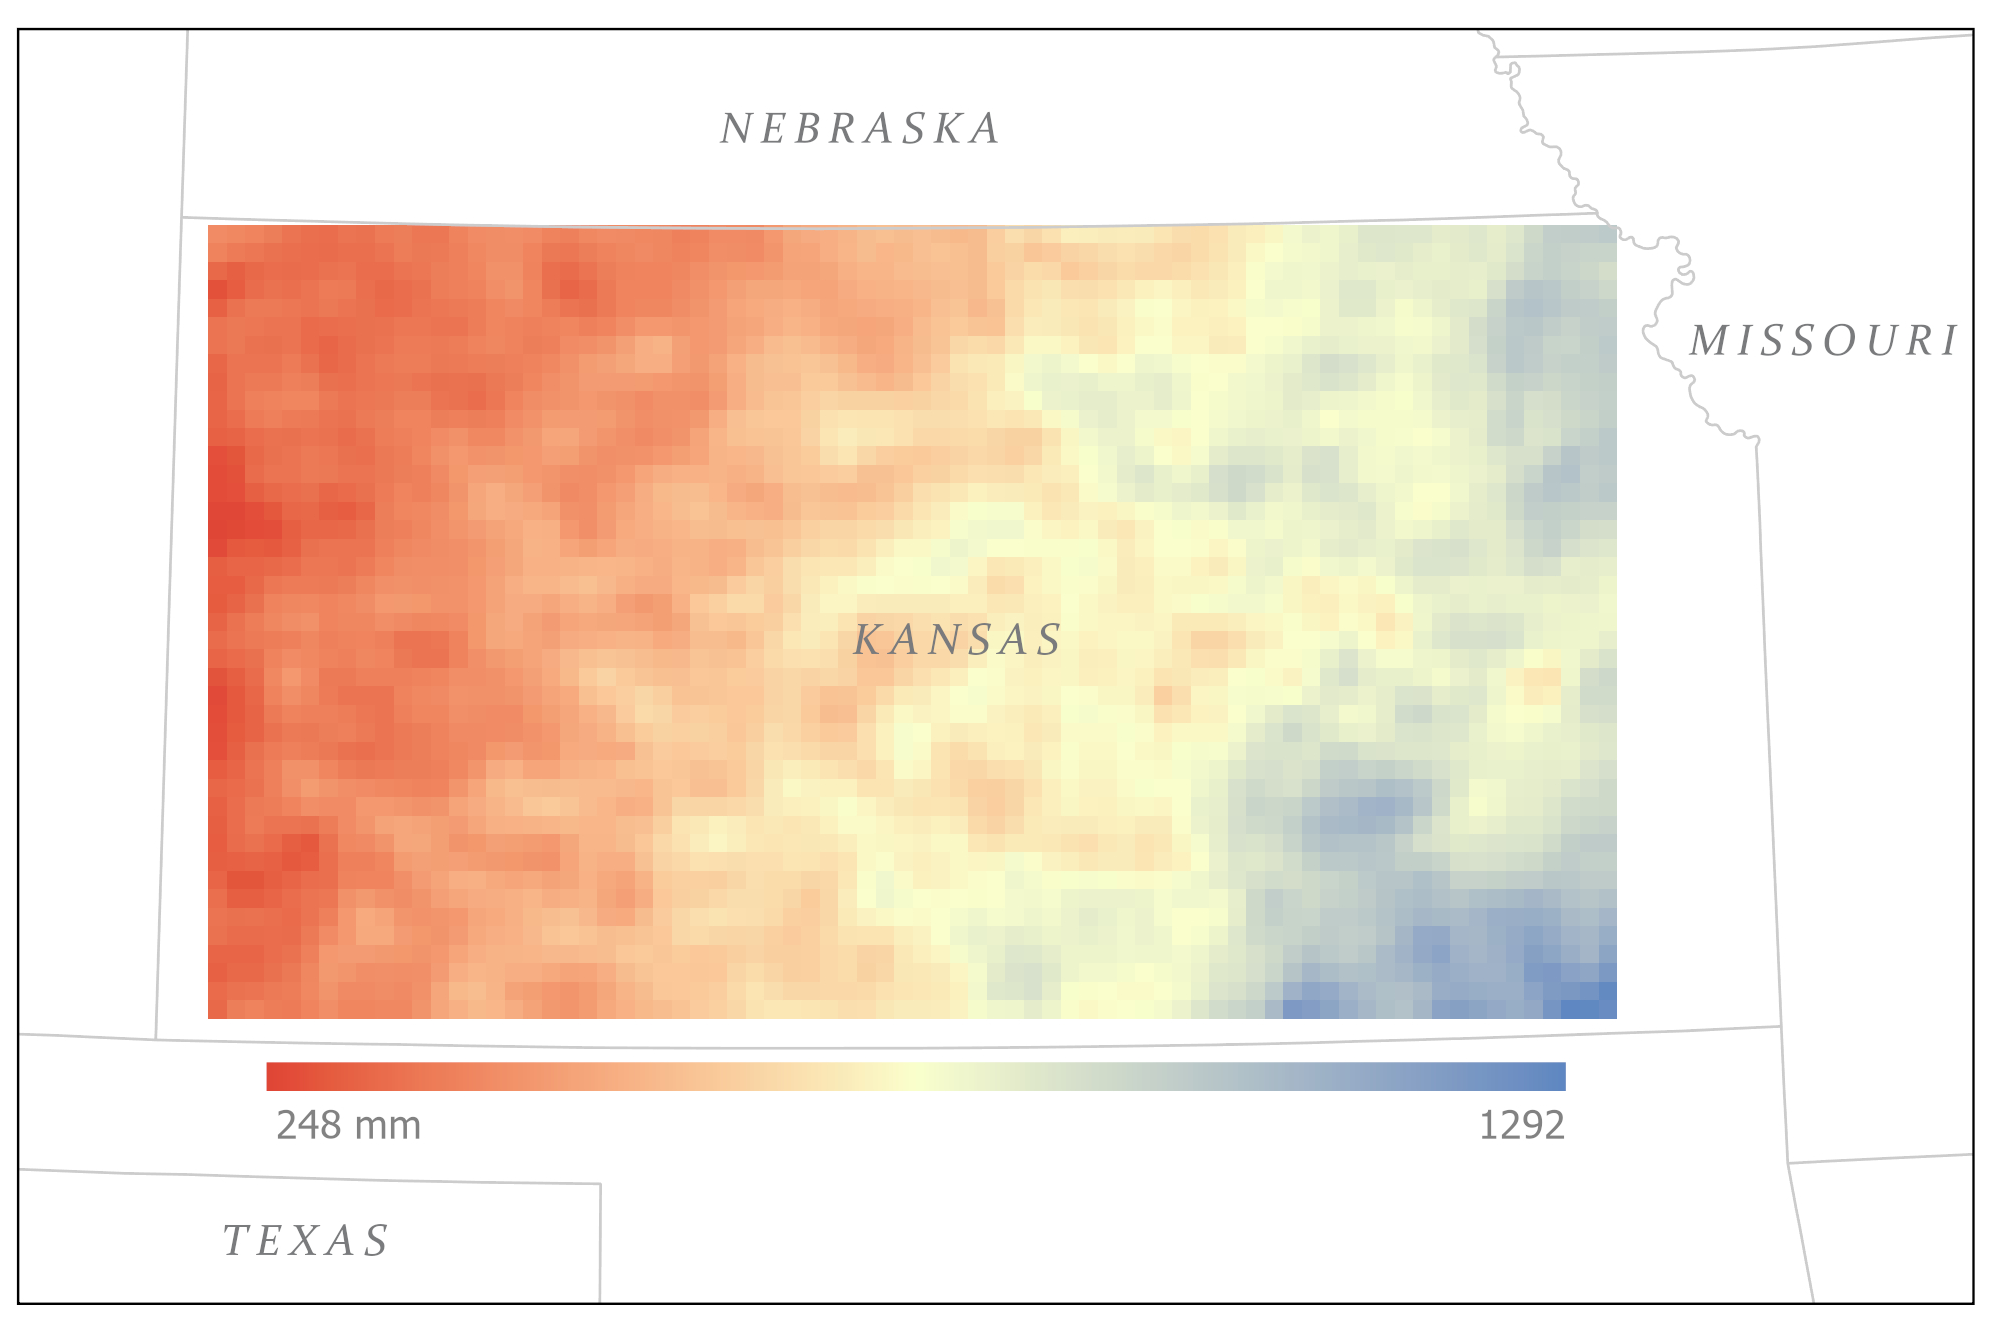
\includegraphics[width=5.20833in,height=\textheight,keepaspectratio]{img/poly_fig1.png}

}

\caption{\label{fig-121}Map of the total 2020 precipitation distribution
for Kansas (USA).}

\end{figure}%

However, we will first focus on the bottom row of pixels which will
provide us with a one-dimensional (east-west) dataset.

\begin{figure}[H]

\centering{

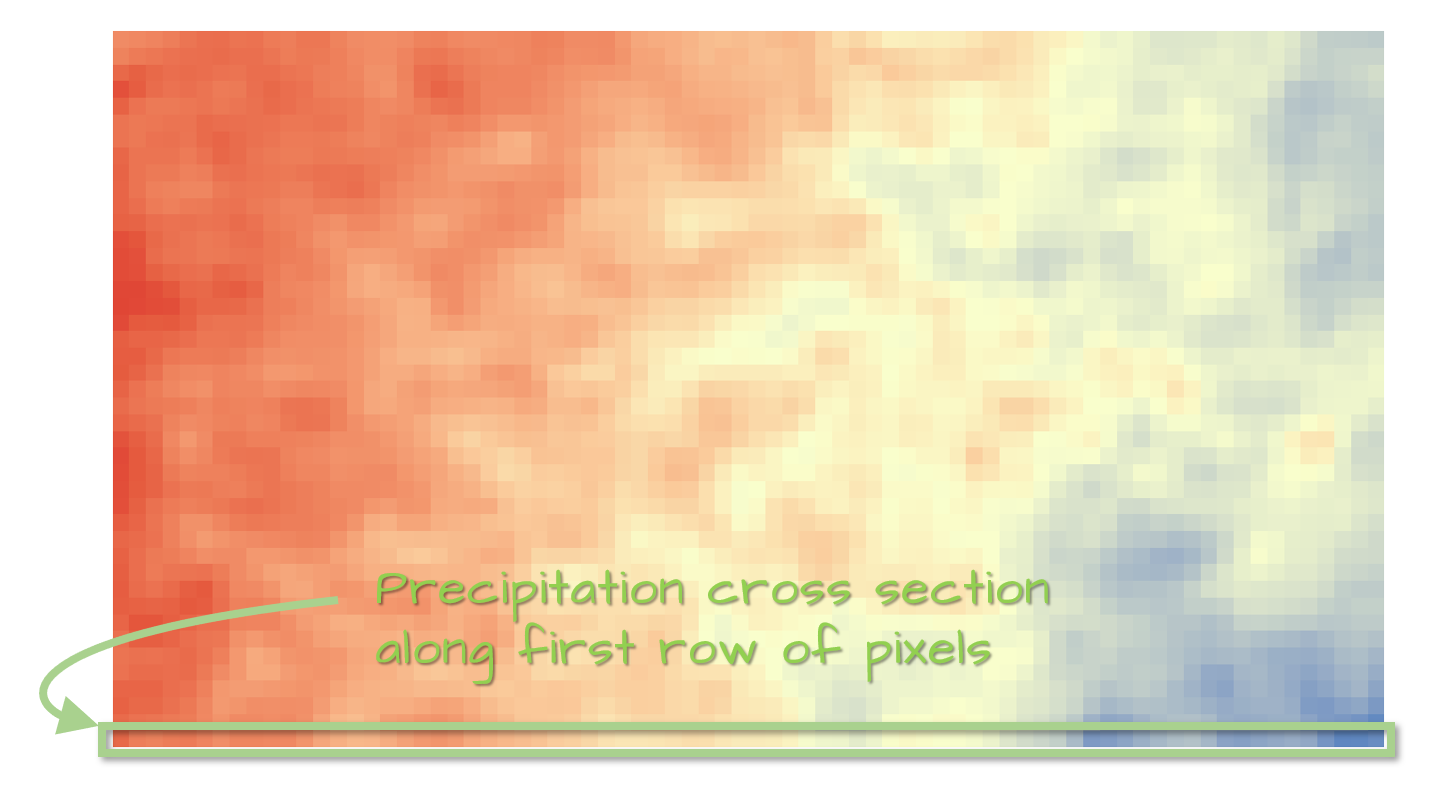
\includegraphics[width=5.20833in,height=\textheight,keepaspectratio]{img/poly_fig2.png}

}

\caption{\label{fig-1211b}Row of pixels used to explore the trend along
a one-dimensional space.}

\end{figure}%

A scatter plot of the precipitation values along the east-west gradient
is shown next. Each point represents the precipitation value at a
specific pixel location.

\begin{figure}[H]

\centering{

\pandocbounded{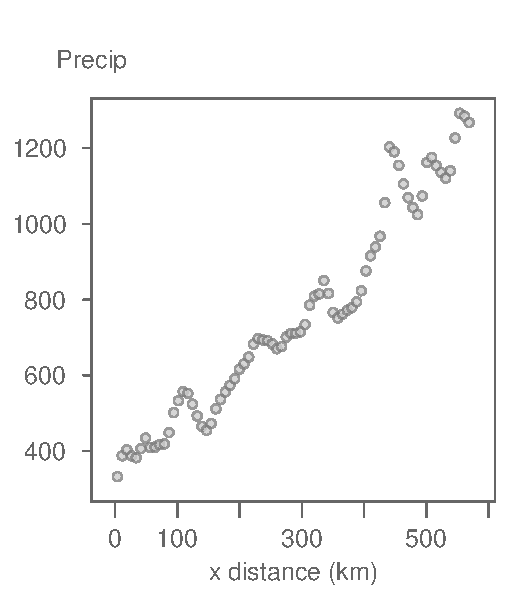
\includegraphics[keepaspectratio]{12_poly_functions_files/figure-pdf/fig-122-1.pdf}}

}

\caption{\label{fig-122}Scatter plot of precipitation along the
east-west gradient defined in Figure~\ref{fig-1211b}.}

\end{figure}%

The simplest model that can be fitted to the data is the mean
precipitation value, a constant. It can be visualized as a horizontal
line. This is also known as a 0\textsuperscript{th} order polynomial
model where:

\begin{equation}
\tag{3}
Precipitation_i = \beta_0  x_i^0 + \varepsilon = \beta_0 + \varepsilon
\end{equation}

Here, \(\beta_0\) is nothing more than the mean precipitation value
(756.8 mm in our working example). Recall that we are only focusing on
the east-west precipitation values, hence the \(y\) coordinate value is
ignored in equation (3).

\begin{figure}[H]

\centering{

\pandocbounded{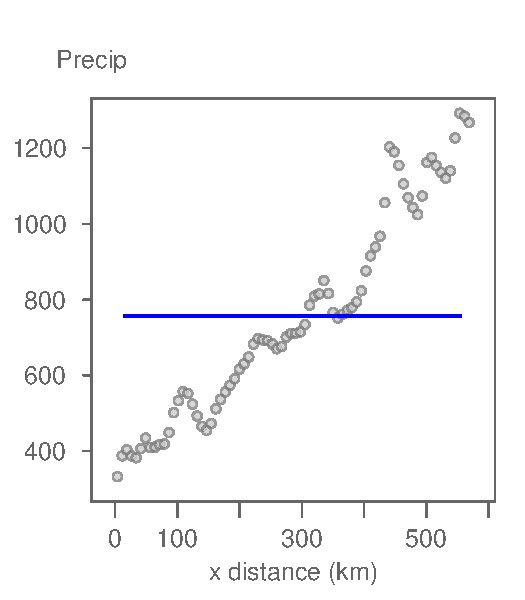
\includegraphics[keepaspectratio]{12_poly_functions_files/figure-pdf/fig-123-1.pdf}}

}

\caption{\label{fig-123}The mean precipitation fitted to the data. This
is the simplest form of a polynomial function where the power is set to
0.}

\end{figure}%

While such a simple model may not prove useful in modeling trends, it
serves as a reference for how well other polynomial models perform.
Model evaluation will be addressed later in this chapter.

It is clear from the plot that the precipitation is far from constant
across the east-west slice of the data. It shows a distinct upward trend
that may be better represented using a sloped line. We can modify the
above model by augmenting the polynomial order:

\begin{equation}
\tag{4}
Precipitation_i = \beta_0 + \beta_1 x_i^1 + \varepsilon_i
\end{equation}

Equation (4) is mathematically defined as a first-order polynomial
model, but it is more often described as a linear trend model. With the
model defined a priori, the model is then fitted to the points.

\begin{figure}[H]

\centering{

\pandocbounded{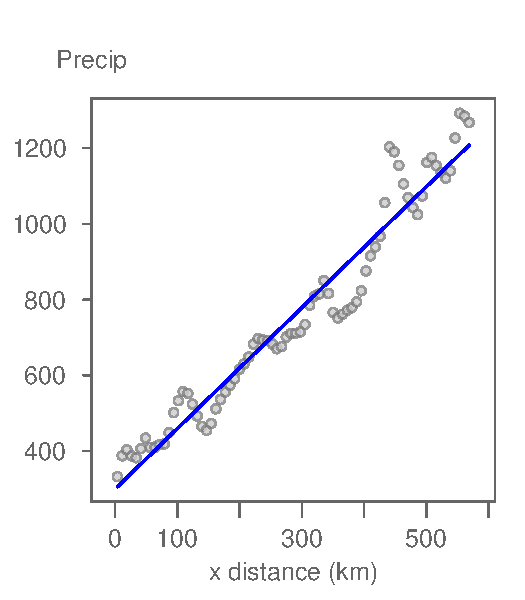
\includegraphics[keepaspectratio]{12_poly_functions_files/figure-pdf/fig-124-1.pdf}}

}

\caption{\label{fig-124}A first-order polynomial function being fitted
to the precipitation data. This is often referred to as a linear trend
model.}

\end{figure}%

There are many approaches to finding the ``best fit'' with the most
popular being the ordinary least squares method. This approach seeks to
minimize the distance between the points and the fitted model when
measured parallel to the y-axis. These are shown as red colored line
segments in the following plot.

\begin{figure}[H]

\centering{

\pandocbounded{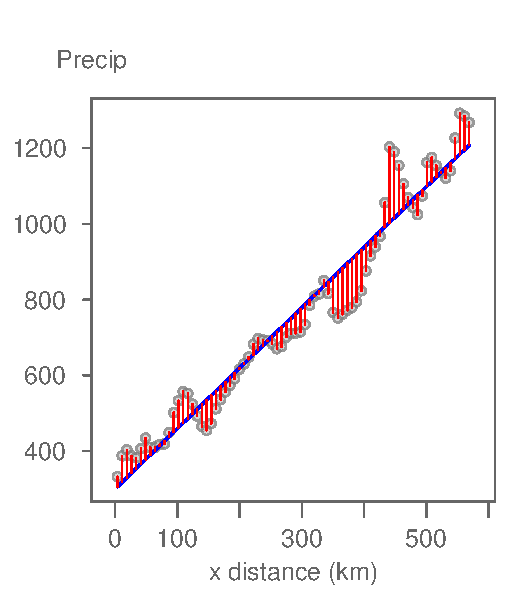
\includegraphics[keepaspectratio]{12_poly_functions_files/figure-pdf/fig-125-1.pdf}}

}

\caption{\label{fig-125}The first-order polynomial function (blue line)
is shown with the residual lines (in red). The function is fitted to the
data in such a way to reduce the sum of the squared residual values.}

\end{figure}%

The distance between the modeled line and each precipitation value is
the residual (\(\varepsilon_i\)). This is part of the data not explained
by the model.

Fitting the first-order polynomial to the data gives us the coefficients
of 305.8 and 1.6 for \(\beta_0\) and \(\beta_1\) respectively.

The \(\beta_1\) coefficient tells us that for every km increase in the
(positive) x direction, precipitation increases by 1.6 mm. Note that the
interpretation of the coefficient is dependent on the mapping units
used. Typically, projection units are in meters or feet. But, when
working at a scale like the State of Kansas, it is best to report
changes in value as a function of larger mapping units such kilometers
or miles.

Statisticians rarely stop at this stage when fitting a model to the
data. It is good practice to plot the residuals against the x value.
This diagnostic plot is useful in assessing if the overall trend in the
data was properly characterized by our polynomial model. To help guide
our eyes, we add a non-parametric curve to the data which does not make
any assumptions about the pattern in the data. Here, we make use of a
loess fit but note that many other non-parametric models can be used for
this purpose.

\begin{figure}[H]

\centering{

\pandocbounded{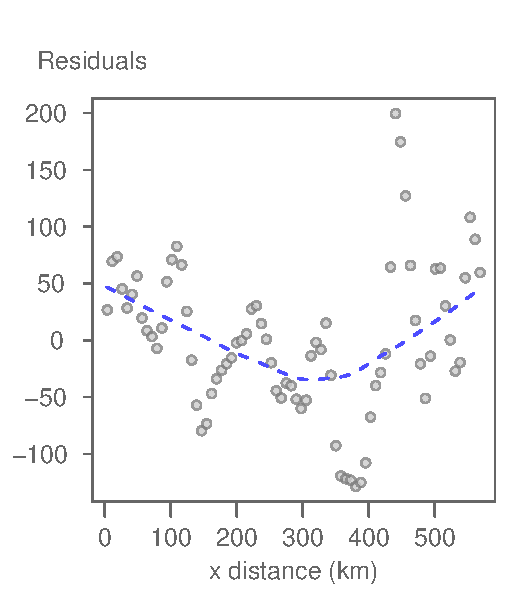
\includegraphics[keepaspectratio]{12_poly_functions_files/figure-pdf/fig-126-1.pdf}}

}

\caption{\label{fig-126}The residuals are checked for any lingering
pattern that may have been missed by the first-order polynomial
function. A non-parametric line such as a loess is used to identify any
pattern in the data.}

\end{figure}%

The diagnostic plot suggests that the first-order polynomial model we
adopted does not fully capture the overall trend in the data. There
appears to be some curvature in the residuals. This may suggest that we
increase the polynomial order by an extra degree.

A second-order polynomial model in a one-dimensional space takes on the
form:

\begin{equation}
\tag{5}
Precipitation_i = \beta_0 + \beta_1 x_i + \beta_2 x_i^2 + \varepsilon_i
\end{equation}

This model generates a curved fit often called a quadratic model.

\begin{figure}[H]

\centering{

\pandocbounded{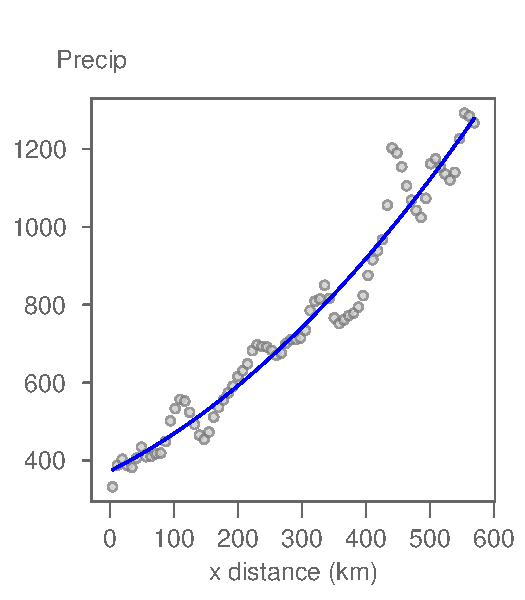
\includegraphics[keepaspectratio]{12_poly_functions_files/figure-pdf/fig-127-1.pdf}}

}

\caption{\label{fig-127}A second-order polynomial function is fitted to
the data. This is also referred to as a quadratic function.}

\end{figure}%

The residual diagnostic plot for this model shows a significant
improvement in that the non-parametric fit (dashed blue line) does not
show an overall trend in the data suggesting that a second-order
polynomial model is a good fit for our data.

\begin{figure}[H]

\centering{

\pandocbounded{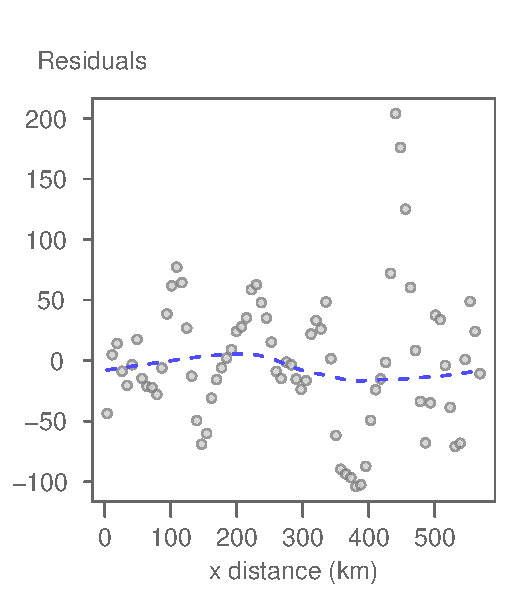
\includegraphics[keepaspectratio]{12_poly_functions_files/figure-pdf/fig-128-1.pdf}}

}

\caption{\label{fig-128}The lack of an overall pattern in the residuals
suggests that the second-order polynomial function does a decent job in
capturing the trend in precipitation.}

\end{figure}%

A unique characteristic of spatial data is the presence of
autocorrelation which is very much apparent in both the original scatter
plot and the diagnostic plot. One might be tempted to try and capture
this non-random pattern in a polynomial model. For example, fitting a
20\textsuperscript{th} order polynomial model would do a decent job in
capturing both the overall trend and localized variation as shown in the
following plot.

\begin{figure}[H]

\centering{

\pandocbounded{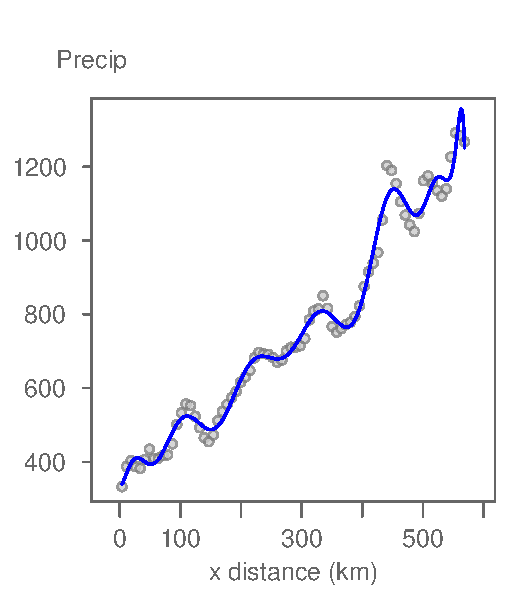
\includegraphics[keepaspectratio]{12_poly_functions_files/figure-pdf/fig-129-1.pdf}}

}

\caption{\label{fig-129}An example of a higher polynomial order function
fitted to the data. This is an example of an overfitted model.}

\end{figure}%

But, doing so is ill-advised. The model has 20 coefficients! Polynomial
models are intended to capture general trends in the data. There are
more sophisticated and specialized statistical methods used to capture
localized spatial autocorrelation as will be demonstrated in the next
chapter. A general rule of thumb is to avoid going above a
3\textsuperscript{rd} order polynomial model. Any higher order model is
likely to capture some aspects of spatial autocorrelation.

\section{Transitioning from a one-dimensional to a two-dimensional
space}\label{transitioning-from-a-one-dimensional-to-a-two-dimensional-space}

The polynomial functions described in the earlier section can easily be
extended to a two-dimensional space. Next, we fit polynomial functions
to the full precipitation extent for the state of Kansas. This adds the
y-coordinate variable to the model.

We learned that the 0\textsuperscript{th} order polynomial is a
horizontal line in one dimensional space. For a two-dimensional space,
this is a horizontal plane that can be defined as:

\begin{equation}
\tag{6}
Precipitation_i = \beta_0 + \beta_1 x_i^0  + \beta_2 y_i^0  + \varepsilon_i = \beta^{'} + \varepsilon_i
\end{equation}

where \(\beta^{'} = (\beta_0 + \beta_1 + \beta_2)\) is the mean
precipitation for the entire study extent (660 mm in our working
example). The following figure shows this plane in a three-dimensional
space.

\begin{figure}[H]

\centering{

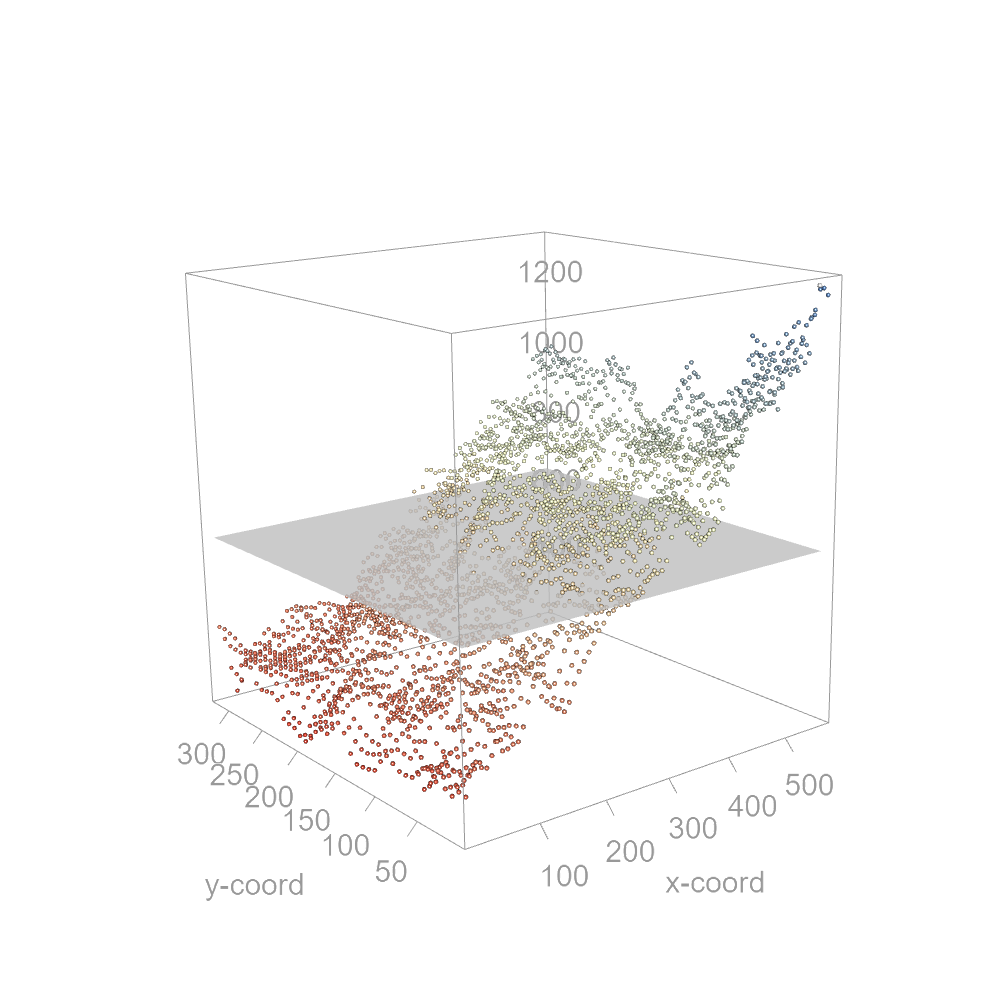
\includegraphics[width=6.25in,height=\textheight,keepaspectratio]{img/poly_fig3.png}

}

\caption{\label{fig-1210a}A 0th order polynomial function fitted to the
full two-dimensional precipitation data. The z-axis is assigned the
precipitation variable.}

\end{figure}%

An east-west trend is apparent in the three-dimensional scatter plot
suggesting that we should seek a first-order polynomial, at the very
least. The model takes on the form:

\begin{equation}
\tag{7}
Precipitation_i = \beta_0 + \beta_1 x_i  + \beta_2 y_i  + \varepsilon_i
\end{equation}

The model defines a plane that can be tilted in any direction. As was
the case with the one-dimensional dataset, we can leverage the least
squares method to fit the model to the data. This results in the
following coefficients:

\begin{equation}
\tag{8}
Precipitation_i = 402 + 1.15 x_i - 0.45 y_i  + \varepsilon_i
\end{equation}

The coefficients tell us by how much the precipitation changes along the
x and y coordinate directions. In our working example, precipitation
increases by 1.15 mm in the x direction (west to east) and decreases by
0.45 mm in the y direction (south to north). The precipitation gradient
is greater in the x-direction than in the y direction. The following
figure shows a three-dimensional rendering of the plane.

\begin{figure}[H]

\centering{

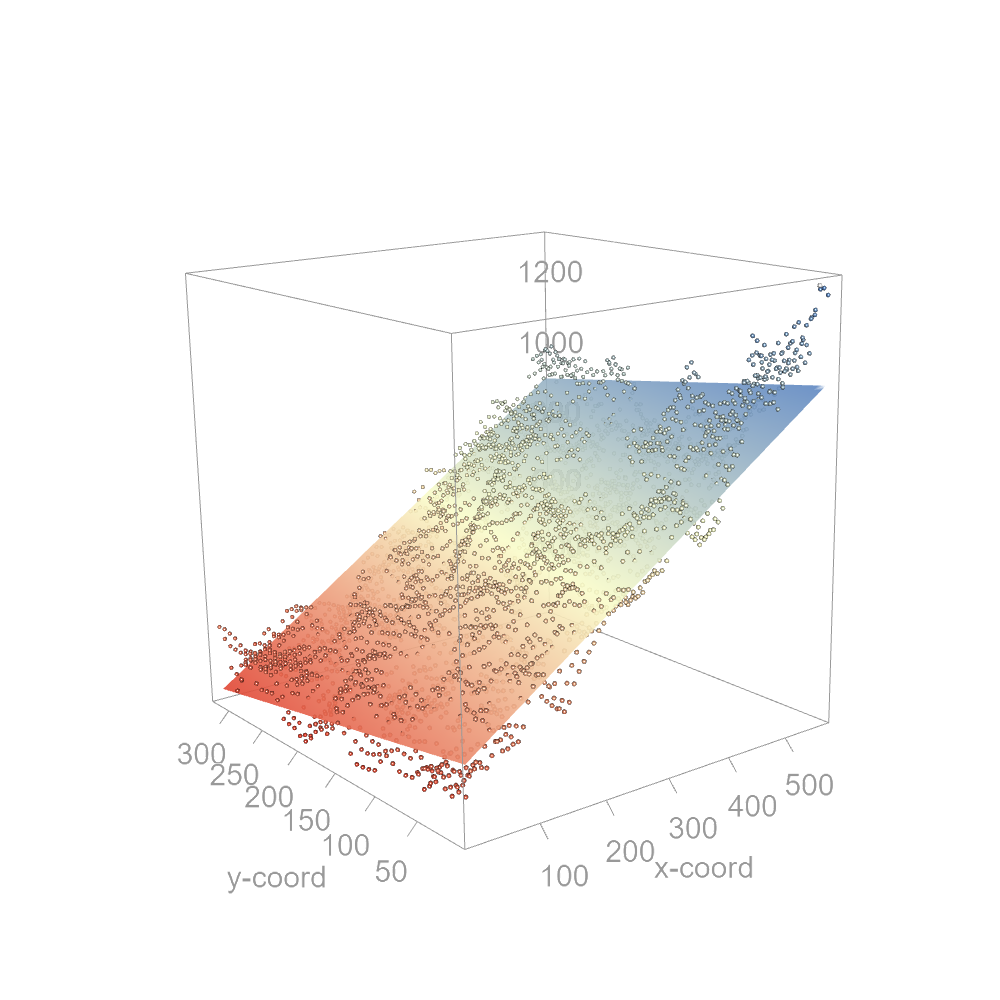
\includegraphics[width=6.25in,height=\textheight,keepaspectratio]{img/poly_fig4.png}

}

\caption{\label{fig-1211}A first-order polynomial function fitted to the
two-dimensional precipitation data.}

\end{figure}%

The same model can be viewed as a two-dimensional raster where each
pixel represents the modeled precipitation.

\begin{figure}[H]

\centering{

\pandocbounded{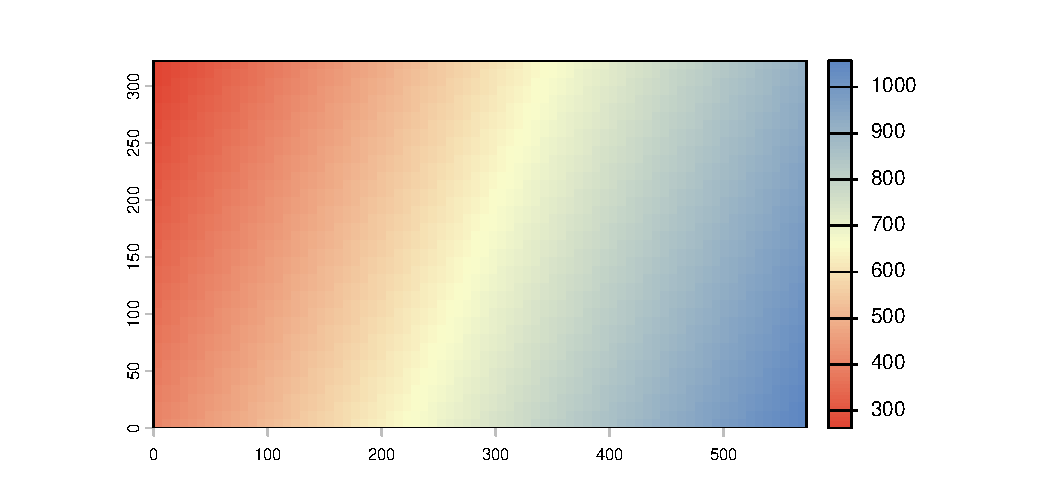
\includegraphics[keepaspectratio]{12_poly_functions_files/figure-pdf/fig-1212-1.pdf}}

}

\caption{\label{fig-1212}A raster view of the first-order polynomial
function shown in Figure Figure~\ref{fig-1211}}

\end{figure}%

How well does the first-order polynomial fit our data? We may first want
to look at the residuals.

\begin{figure}[H]

\centering{

\pandocbounded{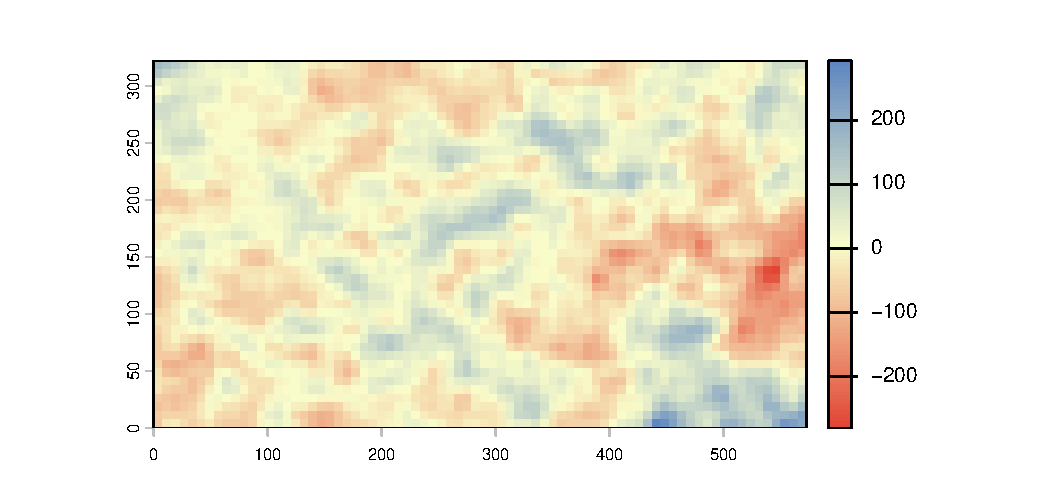
\includegraphics[keepaspectratio]{12_poly_functions_files/figure-pdf/fig-1213-1.pdf}}

}

\caption{\label{fig-1213}The residuals from the fitting of the
first-order polynomial function. Note the cluster of low precipitation
values revealed by removing the trend.}

\end{figure}%

The overall trend observed in the original raster is no longer obvious.
However, subtle trends are more difficult to make out when viewing a
two-dimensional dataset than a one-dimensional dataset. A more effective
way to assess model fit in two-dimensional space is to split the
residuals into their x and y coordinate components by plotting the
residuals as a function of x and y respectively.

\begin{figure}[H]

\centering{

\pandocbounded{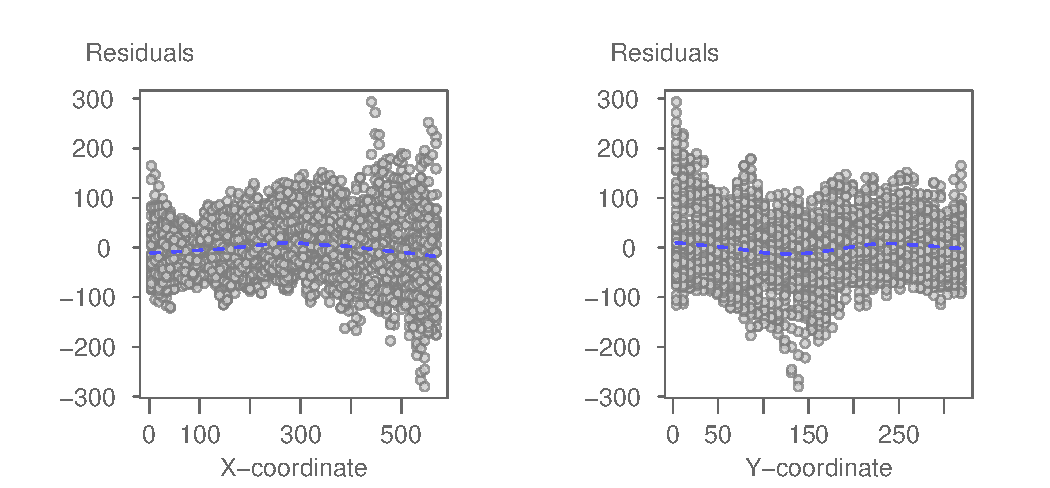
\includegraphics[keepaspectratio]{12_poly_functions_files/figure-pdf/fig-1214-1.pdf}}

}

\caption{\label{fig-1214}The residuals from the fitting of the
first-order polynomial function as viewed from the x-coordinate axis and
the y-coordinate axis.}

\end{figure}%

The plots suggest a very mild curvature in the residuals along the x
coordinate. A similar, but more complex curvature can be observed along
the y-coordinate. It may be worthwhile to augment the function by
another polynomial order giving us a second-order polynomial function to
see if it removes some of these trends. Such a function is also called a
quadratic polynomial function. It takes on the form:

\begin{equation}
\tag{9}
Precipitation_i = \beta_0 + \beta_1 x_i  + \beta_2 y_i + \beta_3 x_i^2  + \beta_4 y_i^2 + \beta_5 x_iy_i + \varepsilon_i
\end{equation}

Note that in addition to adding the squared coordinate values, the
function also adds the interactive terms \(xy\). The interaction term
captures situations where the coefficients for \(x\) or \(y\) are no
longer a constant. For example, if the effect of the x coordinate value
on precipitation changes as a function of changing y coordinate values,
then x's coefficient can no longer be deemed a constant. This is
captured by the \(x_iy_i\) term in equation 9.

The least squares method can be used to fit the function to the data. In
our example, this gives us:

\begin{equation}
\tag{10}
Precipitation_i = 378 + 1.43 x_i -0.66 y_i -0.0003 x_i^2 +0.0013 y_i^2 -0.0005 x_iy_i + \varepsilon_i
\end{equation}

The coefficients suggest that the \(x_i\) and \(y_i\) coordinate values
have a greater influence on the estimate of precipitation than their
\(x_i^2\) and \(y_i^2\) counterparts despite the \(x\) and \(y\) terms
being raised to the power of 2. Note too that the exceedingly small
\(x_iy_i\) coefficient suggests little to no interaction between the
\(x_i\) and \(y_i\) coordinate values.

The next figure shows this curved surface in a three-dimensional space.

\begin{figure}[H]

\centering{

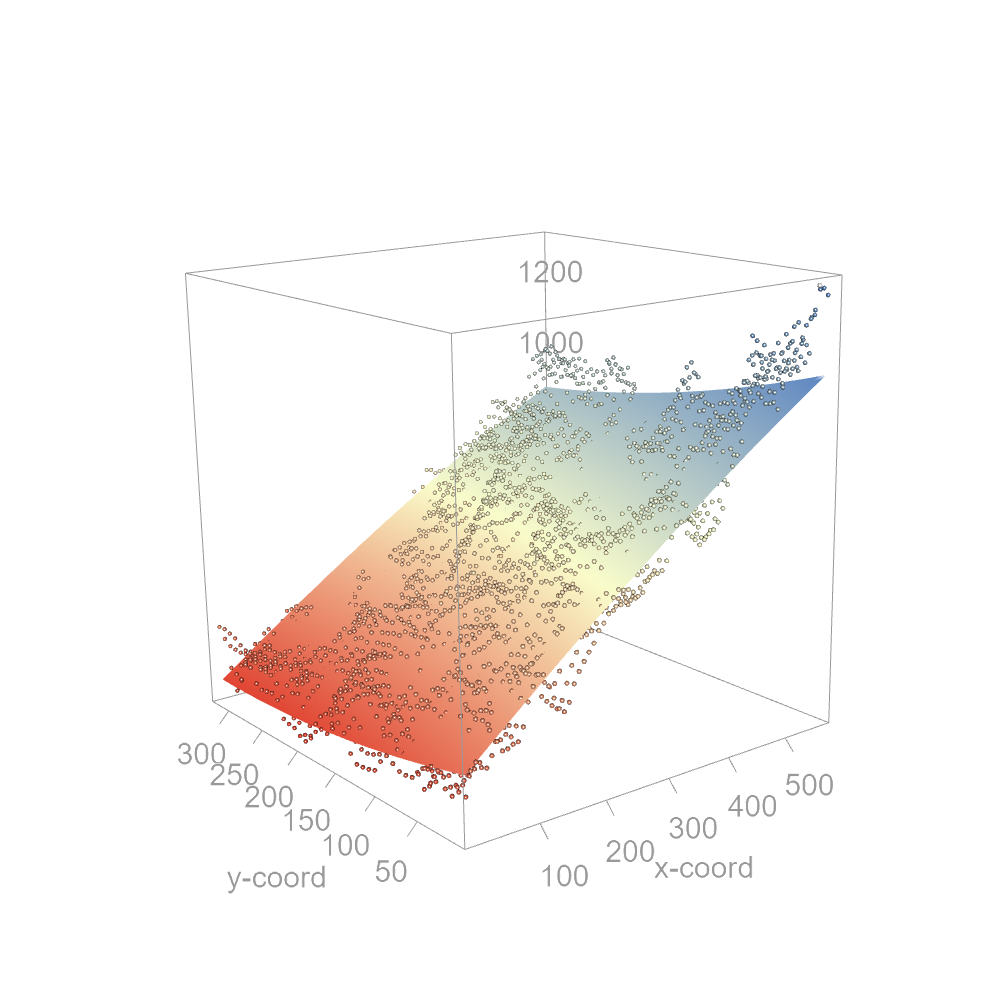
\includegraphics[width=6.25in,height=\textheight,keepaspectratio]{img/poly_fig5.png}

}

\caption{\label{fig-1215}A second-order polynomial function fitted to
the precipitation data. Note the slight curvature in the trend.}

\end{figure}%

The next figure shows the quadratic surface as a two-dimensional raster.

\begin{figure}[H]

\centering{

\pandocbounded{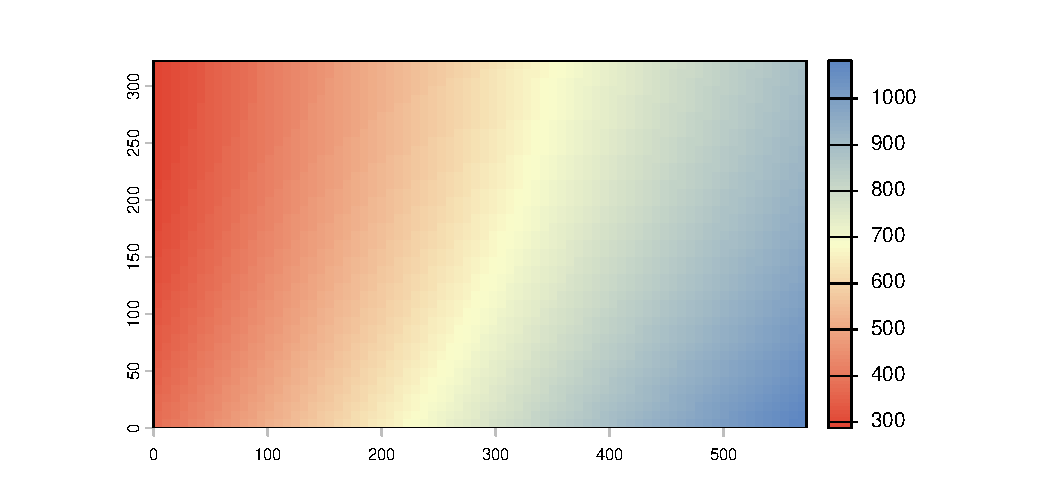
\includegraphics[keepaspectratio]{12_poly_functions_files/figure-pdf/fig-1216-1.pdf}}

}

\caption{\label{fig-1216}A raster view of the second-order polynomial
function shown in Figure~\ref{fig-1215}.}

\end{figure}%

Note that the resulting residuals look barely different from those of
the 1st order polynomial model.

\begin{figure}[H]

\centering{

\pandocbounded{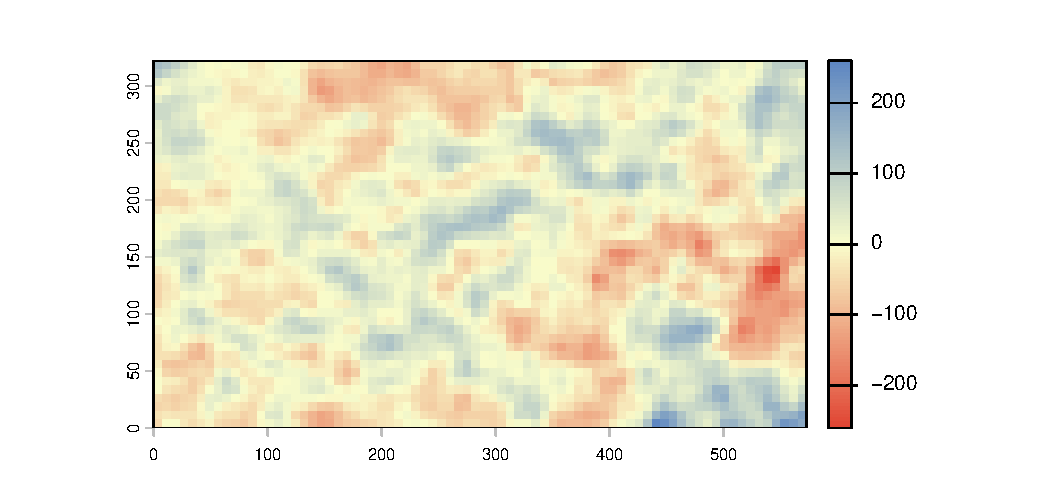
\includegraphics[keepaspectratio]{12_poly_functions_files/figure-pdf/fig-1218-1.pdf}}

}

\caption{\label{fig-1218}The residuals from the fitting of the
second-order polynomial function.}

\end{figure}%

It is therefore best to assess the goodness of fit by plotting the
residuals against the x and y coordinate values.

\begin{figure}[H]

\centering{

\pandocbounded{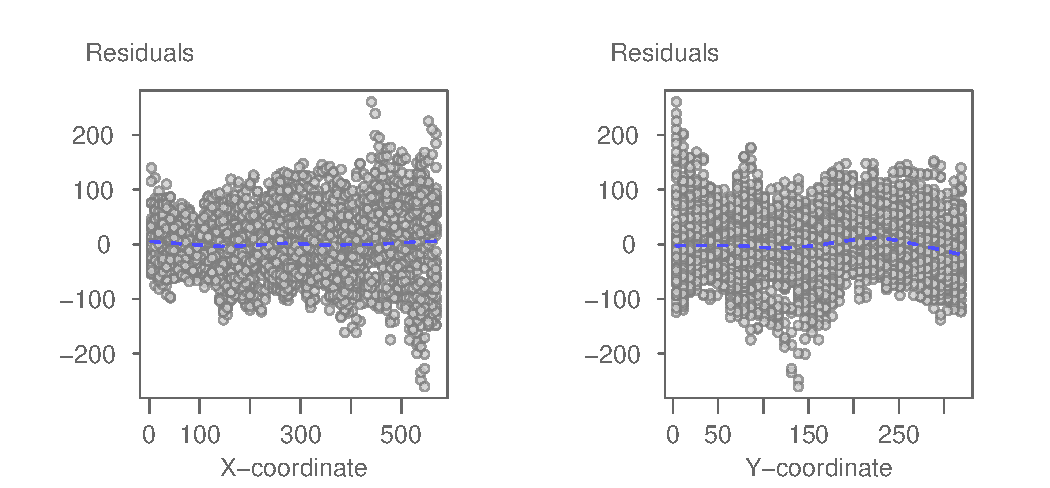
\includegraphics[keepaspectratio]{12_poly_functions_files/figure-pdf/fig-1219-1.pdf}}

}

\caption{\label{fig-1219}The residuals from the fitting of the
second-order polynomial function as viewed from the x-coordinate axis
and the y-coordinate axis.}

\end{figure}%

The second-order polynomial is an improvement over the first-order
polynomial, especially along the x-coordinate axis where the slight
curvature observed in the first-order polynomial model's residuals is no
longer apparent. Note that the range of residual values are also
slightly less with the 2\textsuperscript{nd} order function versus the
first-order function.

Mathematically, there is no limit to the polynomial order you choose.
For example, you could explore a third order polynomial function (a
cubic polynomial) or even a fourth order polynomial function (a quartic
polynomial). But, as was forewarned with the one-dimensional analysis
presented earlier in this chapter, doing so increases the chance of
overfitting the data. Recall that the purpose of modeling the trend is
to capture the data's \emph{overall} pattern. Polynomial functions are
not intended to capturing \emph{local} variability in the data.

One option that may help eliminate the need for higher polynomial orders
is to transform (aka re-express) the variable \(z_i\). Transforming the
data can render a curvilinear function straight (or flat in a
two-dimensional space). Transforming the variable may also be
scientifically justified. There are many datasets that benefit from a
non-linear scale. For example, earthquake magnitudes are measured on a
log scale and some count datasets can benefit from a square root
transformation.

\section{Evaluating a model's goodness of
fit}\label{evaluating-a-models-goodness-of-fit}

The diagnostic plots have, so far, been visual. We can adopt a more
rigorous and systematic approach to evaluating how well the functions
fit the data. A popular statistical measure of ``fit'' is the
coefficient of determination, \(R^2\). It is computed by subtracting one
from the ratio of the sum of residuals squared in the fitted model to
the sum of residuals squared one would get if we had fitted the mean
value.

\begin{equation}
\tag{11}
R^2 = 1 - \frac{\sum(residuals_{model})^2}{\sum(residuals_{mean})^2}
\end{equation}

If the residuals from the model are smaller than those we would have
gotten if we adopted the simpler mean model, \(R^2\) ends up being
large. \(R^2\) ranges from 0 (no improvement whatsoever over the mean)
to 1 (a perfect fit where the residuals from the fitted model are zero).
In our working example, the first-order polynomial model resulted in an
\(R^2\) of 0.87. The second-order polynomial resulted in an \(R^2\) of
0.90, a slight improvement over the first-order polynomial. Note that
the \(R^2\) value is sometimes reported as a percentage rather than a
fraction.

\section{A note about adopting traditional statistical measures of
significance to spatial
functions}\label{a-note-about-adopting-traditional-statistical-measures-of-significance-to-spatial-functions}

Because underlying residuals are likely to exhibit spatial
autocorrelation, traditional methods used to assess ``statistical
significance'' of a model and its coefficient should be avoided. For
example, the cluster of low residual values in the eastern part of
Kansas is a good indication that spatial autocorrelation is present in
our data.

\section{Summary}\label{summary-10}

This chapter introduced polynomial functions as a parametric tool for
modeling first-order spatial effects, the broad location-driven
variation in spatial data. Polynomial models, often referred to as
\textbf{trend surfaces}, describe large-scale spatial patterns as a
function of geographic coordinates and are commonly applied to
continuous spatial fields such as precipitation, elevation, and
population density.

\begin{itemize}
\tightlist
\item
  Trend surfaces are \textbf{polynomial functions} fitted to spatial
  coordinates and used to model broad spatial variation across a study
  area.
\item
  Polynomial models are most useful for characterizing
  \textbf{first-order effects}, or large-scale spatial trends associated
  with absolute location.
\item
  Trend surfaces can be fitted in one or two-dimensional space using
  regression techniques such as ordinary least squares. Increasing the
  polynomial order allows more complex trends to be modeled, but
  excessively high orders can lead to \textbf{overfitting} and may begin
  capturing \textbf{local spatial variation} rather than the underlying
  trend.
\item
  \textbf{Residuals} represent the portion of the data not explained by
  the trend surface and provide an important diagnostic tool for
  evaluating model performance.
\item
  The primary goal of trend modeling is not to explain all variation in
  the data, but rather to account for broad spatial trends and isolate
  the remaining unexplained variation.
\item
  Once a first-order trend has been modeled and removed, the residuals
  can be examined for \textbf{remaining spatial structure}. Determining
  whether neighboring residuals are more similar (or dissimilar) than
  expected by chance leads directly to the study of spatial
  autocorrelation, the principal second-order effect examined in the
  next chapter.
\end{itemize}

\chapter{Spatial Autocorrelation}\label{spatial-autocorrelation}

\section{Introduction}\label{introduction-12}

In the previous chapter, we explored how polynomial functions can be
used to model spatial trends that capture broad, location-driven
variation in continuous spatial fields. By fitting and removing global
trends, we revealed residuals that may still exhibit spatial structure.
This chapter builds on that foundation by introducing \textbf{spatial
autocorrelation}, a second-order property that describes how values at
one location relate to values at nearby locations.

This concept is rooted in \textbf{Tobler's First Law of Geography} which
states:

\begin{quote}
\emph{``The first law of geography: Everything is related to everything
else, but near things are more related than distant things.''} Waldo R.
Tobler (Tobler 1970)
\end{quote}

This principle raises an important question: \emph{How can we determine
whether nearby locations are actually more similar than we would expect
under a random spatial arrangement?} Spatial autocorrelation provides a
statistical framework for quantifying and testing such spatial
dependence. In this chapter, we focus on Moran's I, one of the most
widely used measures of spatial autocorrelation.

\begin{figure}[H]

\centering{


\includegraphics[width=6.25in,height=\textheight,keepaspectratio]{img/Random_maps.png}

}

\caption{\label{fig-rand_maps}Conceptual illustration of spatial
autocorrelation. Geographic variables such as population density and
elevation typically exhibit spatial structure (left). Randomly
rearranging the same values across space removes that structure
(right).}

\end{figure}%

As illustrated in Figure~\ref{fig-rand_maps}, many geographic variables
exhibit broad areas of similar values. If the same values were
distributed independently across space, the resulting maps would appear
much more fragmented.

To make the mathematical foundations of autocorrelation more accessible,
we shift from the raster-based data used in the previous chapter to a
simpler dataset composed of \textbf{polygonal areal units} (e.g.,
counties). This allows us to clearly illustrate how spatial
relationships are defined, how spatial weights are constructed, and how
measures like \textbf{Moran's I} are computed.

This chapter focuses on:

\begin{itemize}
\tightlist
\item
  Defining spatial autocorrelation and its role in spatial statistics.
\item
  Constructing spatial weights to represent neighborhood relationships.
\item
  Computing and interpreting \textbf{global} and \textbf{local Moran's
  I} statistics.
\item
  Using permutation-based hypothesis testing to assess significance.
\end{itemize}

\section{\texorpdfstring{Global Moran's
\emph{I}}{Global Moran's I}}\label{global-morans-i}

While maps can sometimes reveal clusters of similar values, visual
interpretation alone cannot tell us how strong those patterns are or
whether they are stronger than we might expect by chance. To move beyond
subjective impressions, we need a quantitative measure of spatial
association. Specifically, we want to quantify the degree to which
similar attribute values are clustered or dispersed across space.

One widely used statistic for this purpose is \textbf{Moran's I} , a
measure of \textbf{global spatial autocorrelation}. It quantifies the
overall tendency for features with similar values to occur near one
another, given a specified definition of neighborhood (e.g., contiguity
or distance). Conceptually, Moran's I measures the relationship between
a variable and a spatially lagged version of that same variable.

\subsection{\texorpdfstring{Computing the Moran's
\emph{I}}{Computing the Moran's I}}\label{computing-the-morans-i}

Let's start with a working example: 2020 median per capita income for
the state of Maine.

\begin{figure}[H]

\centering{

\pandocbounded{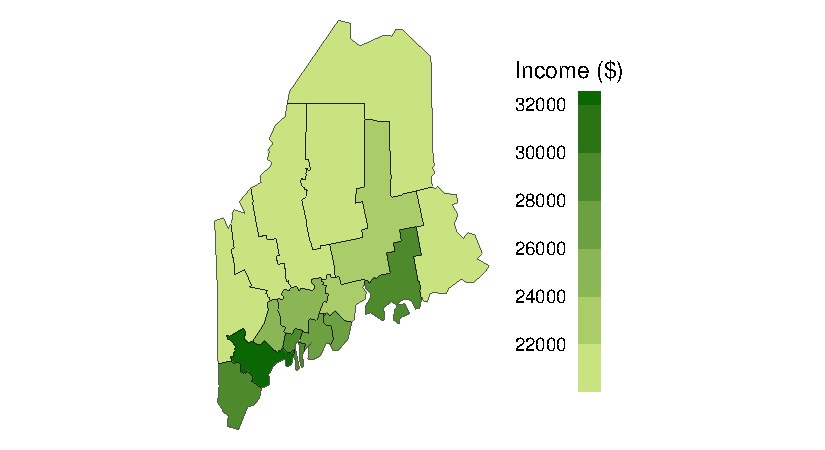
\includegraphics[keepaspectratio]{13_autocorrelation_files/figure-pdf/fig-map03-1.pdf}}

}

\caption{\label{fig-map03}Map of 2020 median per capita income for Maine
counties (USA).}

\end{figure}%

At first glance, the county-level income distribution appears clustered,
with high-income counties tending to occur near other high-income
counties and low-income counties tending to occur near other low-income
counties. However, visual inspection alone cannot tell us how strong
this apparent clustering is, nor whether it reflects a meaningful
spatial process. To move beyond a qualitative assessment, we need a
quantitative measure of the degree to which similar (or dissimilar)
values occur near one another. One of the most widely used measures for
this purpose is the \textbf{Moran's I statistic}.

\begin{quote}
\textbf{Trend versus Autocorrelation}\\
The pattern shown in Figure~\ref{fig-map03} may reflect a broad spatial
trend (a first-order effect), local spatial dependence (a second-order
effect), or both. In practice, analysts often assess spatial
autocorrelation using the residuals remaining after a first-order trend
has been modeled and removed. For pedagogical simplicity, we set that
complication aside here and apply Moran's I directly to the observed
income values.
\end{quote}

The Moran's \emph{I} statistic is a measure of spatial autocorrelation
that quantifies the degree to which similar values (like income) cluster
together in space. It is computed as the correlation between a variable
and its spatially lagged counterpart, based on a defined spatial weights
matrix.

But before we go about computing this correlation, we need to come up
with a way to define a neighbor. One approach is to define a neighbor as
being any contiguous polygon. For example, the northernmost county
(Aroostook), has four contiguous neighbors while the southern most
county (York) has just two contiguous counties. Other neighborhood
definitions can include distance bands (e.g.~counties within 100 km) and
k nearest neighbors (e.g.~the 2 closest neighbors). Note that distance
bands and k nearest neighbors are usually measured using the polygon's
centroids and not their boundaries.

\begin{figure}[H]

\centering{


\includegraphics[width=6.25in,height=\textheight,keepaspectratio]{img/Diff_neighbors.png}

}

\caption{\label{fig-map04}Three alternative ways of defining neighbors:
contiguity, distance bands, and k nearest neighbors. The choice of
neighborhood definition determines which features interact in the
autocorrelation analysis and can influence the resulting Moran's I
statistic. Orange numbers indicate the number of neighbors associated
with each county.}

\end{figure}%

Once we've defined a neighborhood structure, we can summarize the
attribute values surrounding each polygon. For example, we might compute
the average income of a polygon's neighbors. This neighborhood summary
is called a \textbf{spatial lag} because it represents the value of the
variable in the surrounding area rather than at the focal polygon
itself. In our working example, we compute the average neighboring
income value (\emph{Income\textsubscript{lag}}) for each county.

If nearby counties tend to have similar incomes, then counties with high
income values should be associated with high lagged-income values, while
counties with low income values should be associated with low
lagged-income values.

We then plot \emph{Income\textsubscript{lag}} against \emph{Income} for
each county. When both variables are standardized (converted to
z-scores), the slope of the fitted regression line is equal to the
Moran's I statistic.

\begin{figure}[H]

\centering{

\pandocbounded{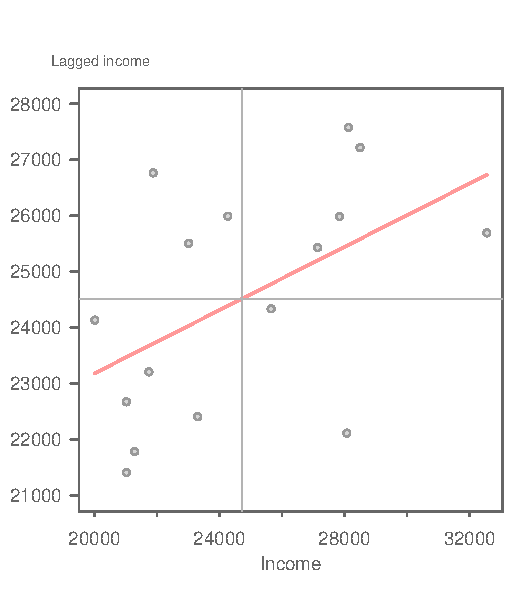
\includegraphics[keepaspectratio]{13_autocorrelation_files/figure-pdf/fig-map05-1.pdf}}

}

\caption{\label{fig-map05}Scatter plot of spatially lagged income
(neighboring income) versus county income. The positive relationship
suggests that counties with similar income values tend to occur near one
another. When both axes are standardized (converted to z-scores), the
slope of the fitted line equals the Moran's \emph{I} statistic.}

\end{figure}%

If there is no degree of association between \emph{Income} and
\emph{Income\textsubscript{lag}}, the slope will be close to flat
(resulting in a Moran's \emph{I} value near 0). In our working example,
the slope is far from flat with a Moran's \emph{I} value of 0.28.
Positive values indicate clustering of similar values, negative values
indicate neighboring dissimilarity, and values near zero suggest little
spatial association. The observed Moran's I value is positive,
suggesting that similar income values tend to occur near one another.
The next question is whether this level of clustering is stronger than
we would expect under a random spatial arrangement. There are two
approaches to estimating the significance: an analytical solution and a
Monte Carlo solution. The analytical solution makes some restrictive
assumptions about the data and thus cannot always be reliable. The other
approach (and the one favored here) is a Monte Carlo test. This approach
avoids parametric assumptions about the data distribution or spatial
layout, relying instead on the assumption that values are exchangeable
under the null hypothesis.

\subsection{Monte Carlo approach to estimating
significance}\label{monte-carlo-approach-to-estimating-significance}

In a Monte Carlo permutation test, we assess the significance of an
observed Moran's \emph{I} statistic by comparing it to a distribution of
values generated under the null hypothesis of spatial randomness. This
is done by \textbf{permuting} the attribute values across spatial units
while keeping the spatial structure (e.g., neighborhood relationships)
fixed.

For each permutation, the attribute values are shuffled among the
polygons and a new Moran's \emph{I} value is computed.

If the observed clustering is no stronger than expected under
randomness, the Moran's I values computed from the permutations should
resemble the observed value. Conversely, if the observed pattern is
unusually clustered, the observed statistic should stand apart from most
of the randomized outcomes.

\begin{figure}[H]

\centering{

\pandocbounded{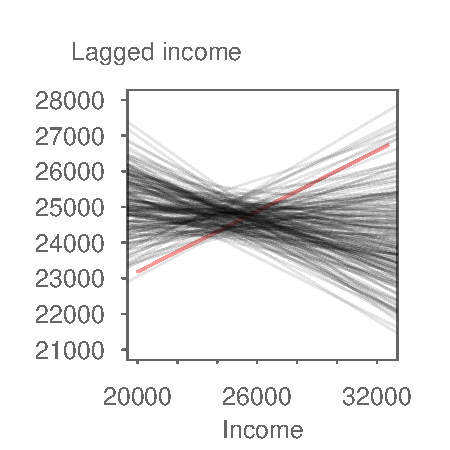
\includegraphics[keepaspectratio]{13_autocorrelation_files/figure-pdf/fig-map06-1.pdf}}

}

\caption{\label{fig-map06}Results from 199 permutations. Plot shows
Moran's \emph{I} lines (in gray) computed from each random permutation
of income values. The observed Moran's \emph{I} line for the original
dataset is shown in red.}

\end{figure}%

Repeating this process many times yields a \textbf{sampling
distribution} of Moran's \emph{I} values that would be expected if the
observed values were randomly distributed across space.

\begin{figure}[H]

\centering{

\pandocbounded{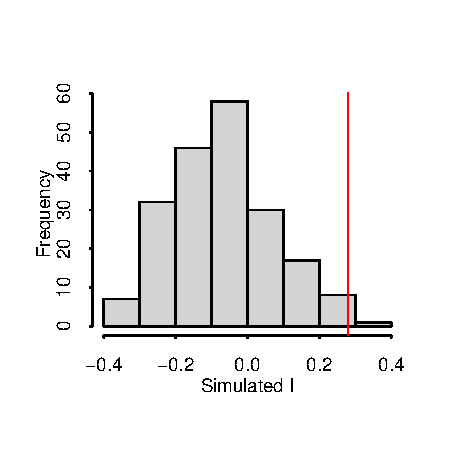
\includegraphics[keepaspectratio]{13_autocorrelation_files/figure-pdf/fig-map07-1.pdf}}

}

\caption{\label{fig-map07}Histogram of Moran's I values generated under
the null hypothesis of spatial randomness. The red line marks the
observed Moran's \emph{I} value (0.28), which lies in the upper tail of
the null distribution.}

\end{figure}%

Notice that most randomized Moran's I values are centered near zero,
which is what we would expect under spatial randomness.

In our working example, the 199 simulations suggest that our observed
Moran's \emph{I} value of 0.28 would be unlikely if the income values
were randomly distributed across counties. A pseudo \emph{p-value} can
be computed as the proportion of simulated Moran's I values that are at
least as extreme as the observed statistic:

\[
\dfrac{N_{extreme}+1}{N+1}
\]

where \(N_{extreme}\) is the number of simulated Moran's \emph{I} values
at least as extreme as the observed statistic and \(N\) is the total
number of simulations. The addition of 1 to both the numerator and
denominator ensures that the observed statistic is included as one of
the possible outcomes and prevents a p-value of exactly zero.

Here, out of 199 simulations, just three simulated \emph{I} values were
more extreme than our observed statistic, \(N_{extreme}\) = 3, so \(p\)
is equal to (3 + 1) / (199 + 1) = 0.02. Because only four of the 200
outcomes (the observed statistic plus three simulated values) were at
least as extreme as the observed Moran's I, the observed pattern would
be unlikely if the income values were randomly distributed across
counties. We therefore have evidence against the null hypothesis of
spatial randomness.

It is important to distinguish permutation tests from other simulation
approaches commonly used in statistics. In this permutation example, we
shuffled the observed income values among polygons without
replacement--this is referred to as a \textbf{permutation-based
randomization}. This should not be confused with a
\textbf{distribution-based simulation} where new values are randomly
generated from a theoretical distribution and assigned to features. In
such a scenario, one chooses to randomly assign a set of values to each
feature in a data layer from a \emph{theorized distribution} (for
example, a \emph{Normal} distribution). This may result in a completely
different set of values for each permutation outcome. Note that you
would only adopt this approach if the theorized distribution
underpinning the value of interest is known \emph{a priori}.

Another important consideration when computing a permutation-based
p-value from a permutation test is the number of simulations to perform.
In the above example we ran 199 permutations, thus, the smallest p-value
we could possibly come up with is 1 / (199 + 1) or a p-value of 0.005.
You should therefore choose a number of permutations, \(N\), large
enough to allow for finer resolution of p-values and more robust
inference.

\section{\texorpdfstring{Moran's \emph{I} at different distance
bands}{Moran's I at different distance bands}}\label{morans-i-at-different-distance-bands}

So far we have defined neighbors using polygon contiguity. While this
approach is common, it implicitly assumes that spatial relationships
operate only among immediately adjacent polygons. In practice, spatial
processes often operate across a range of distances. This raises an
important question: at what spatial scale is autocorrelation strongest?
One way to explore this question is to compute Moran's I repeatedly
using different distance-based neighborhood definitions.

The procedure is conceptually identical to the one used earlier, except
that the neighborhood definition changes from one analysis to the next.
The steps for this type of analysis are straightforward:

\begin{enumerate}
\def\labelenumi{\arabic{enumi}.}
\tightlist
\item
  Define a neighborhood structure based on a specific distance band.
\item
  Compute lagged values for the defined set of neighbors.
\item
  Calculate the Moran's \emph{I} value for the defined neighborhood.
\item
  Repeat for additional distance bands to observe how autocorrelation
  changes with spatial scale.
\end{enumerate}

For example, the Moran's \emph{I} values for income distribution in the
state of Maine at distances of 75, 125, up to 325 km are presented in
the following plot:

\begin{figure}[H]

\centering{


\includegraphics[width=5.20833in,height=\textheight,keepaspectratio]{img/MoranI_distance_band.png}

}

\caption{\label{fig-mc_distance}Moran's \emph{I} computed at increasing
distance bands. Positive values indicate that counties separated by
those distances tend to have similar incomes, while negative values
indicate dissimilarity. Red points mark statistically significant Moran
\emph{I} values (p ≤ 0.05).}

\end{figure}%

The plot suggests that there is significant spatial autocorrelation
between counties within 75 km of one another, but as the distances
between counties increase, autocorrelation shifts from positive to
negative, indicating that nearby counties tend to have similar income
levels, while counties farther apart tend to be more dissimilar. This
pattern is consistent with Tobler's First Law: nearby counties tend to
be more similar than distant counties. Beyond a certain distance,
however, income values become increasingly dissimilar, leading to
negative autocorrelation.

\section{\texorpdfstring{Local Moran's
\emph{I}}{Local Moran's I}}\label{local-morans-i}

The global Moran's I statistic summarizes spatial autocorrelation across
the entire study area. While useful, it does not tell us \emph{where}
clusters of similar or dissimilar values occur. To identify these local
patterns, we can decompose the global statistic into a set of localized
measures of autocorrelation. This is commonly referred to as
\textbf{Local Moran's I}.

A local Moran's \emph{I} analysis is best suited for relatively large
datasets, particularly when hypothesis testing is of interest. We
therefore switch to a different dataset: household income data for
Massachusetts (USA), aggregated to U.S. Census county subdivisions. As
with the Maine example, we temporarily ignore potential first-order
trends for pedagogical simplicity and apply the analysis directly to the
observed values.

\begin{figure}[H]

\centering{

\pandocbounded{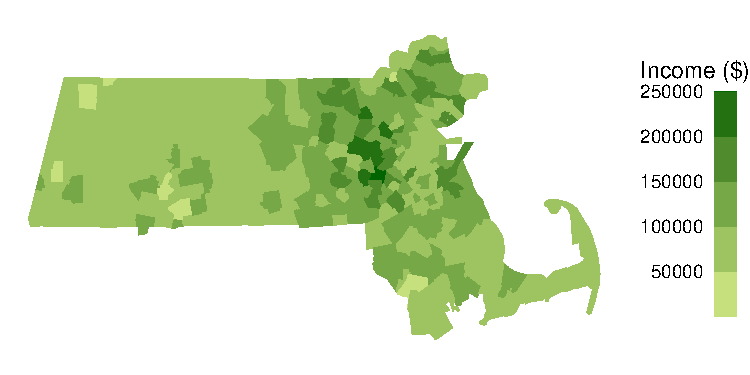
\includegraphics[keepaspectratio]{13_autocorrelation_files/figure-pdf/fig-dataset-1.pdf}}

}

\caption{\label{fig-dataset}Median household income for Massachusetts
county subdivisions in 2020. The large number of spatial units makes
this dataset well suited for exploring localized patterns of spatial
autocorrelation.}

\end{figure}%

Applying a contiguity-based neighborhood definition, we compute the
average neighboring income value (\emph{Income lag}) for each county
subdivision and plot it against the subdivision's own income value. As
with the Global Moran's I analysis, this scatterplot compares each
observation to its surrounding neighborhood. However, rather than
focusing on the overall slope of the point cloud, we are now interested
in the position of individual points because they help reveal localized
patterns of spatial association.

\begin{figure}[H]

\centering{

\pandocbounded{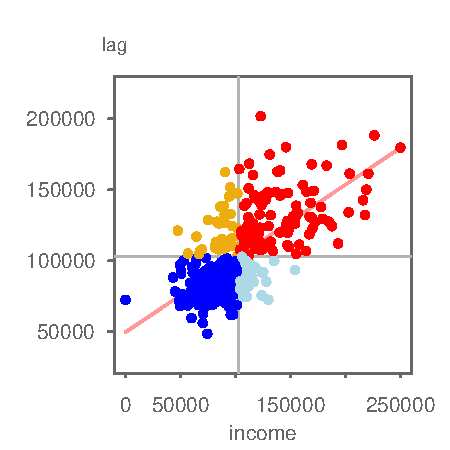
\includegraphics[keepaspectratio]{13_autocorrelation_files/figure-pdf/fig-chunk10-1.pdf}}

}

\caption{\label{fig-chunk10}Moran scatterplot of median household income
versus spatially lagged income for Massachusetts county subdivisions.}

\end{figure}%

The vertical and horizontal reference lines mark the mean values for
income and lagged income, respectively, dividing the scatterplot into
four quadrants. Observations in the upper-right quadrant represent high
values surrounded by high values (\textbf{high-high}) and are shown in
red. Observations in the lower-left quadrant represent low values
surrounded by low values (\textbf{low-low}) and are shown in dark blue.
The remaining quadrants identify spatial outliers: high values
surrounded by low values (\textbf{high-low}, light blue) and low values
surrounded by high values (\textbf{low-high}, orange).

The quadrant classifications shown in the Moran scatterplot
(Figure~\ref{fig-chunk10}) can be mapped back to their corresponding
county subdivisions. This allows us to identify where high-high,
low-low, high-low, and low-high spatial relationships occur across the
study area.

\begin{figure}[H]

\centering{

\pandocbounded{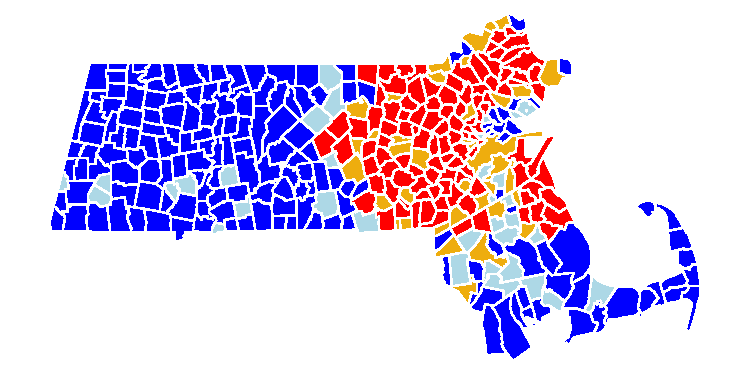
\includegraphics[keepaspectratio]{13_autocorrelation_files/figure-pdf/fig-map10-1.pdf}}

}

\caption{\label{fig-map10}Spatial distribution of the four Moran
scatterplot quadrants. High-high and low-low polygons indicate local
similarity, while high-low and low-high polygons indicate local spatial
outliers.}

\end{figure}%

The Moran scatterplot and corresponding map help identify
\emph{potential} local clusters and spatial outliers. However, visual
classification alone does not tell us whether these local patterns are
stronger than we might expect under a random spatial arrangement. Each
spatial unit therefore has its own Local Moran's I statistic, denoted
\(I_i\), which quantifies the degree of spatial autocorrelation around
that unit. The calculation of \(I_i\) is shown later in the chapter.

\subsection{Significance Testing for Local Moran's
I}\label{significance-testing-for-local-morans-i}

While the scatterplot helps visually identify potential clusters,
statistical significance must be assessed to determine whether these
patterns are likely to have occurred by chance.

As with the global Moran's \emph{I}, there is both an analytical and a
Monte Carlo approach to assessing the significance of \(I_i\). In a
Monte Carlo approach, the value of the focal feature remains fixed while
the values of all other features are repeatedly shuffled among
locations. After each permutation, a new \(I_i\) is computed using the
randomized neighborhood values. Repeating this process many times
generates a reference distribution of \(I_i\) values that we would
expect if the observed values were randomly distributed across the study
area.

To illustrate, consider a polygon in eastern Massachusetts with a high
observed \(I_i\) value. We assess its significance by comparing it to a
distribution of \(I_i\) values generated through permutation.

\begin{figure}[H]

\centering{

\pandocbounded{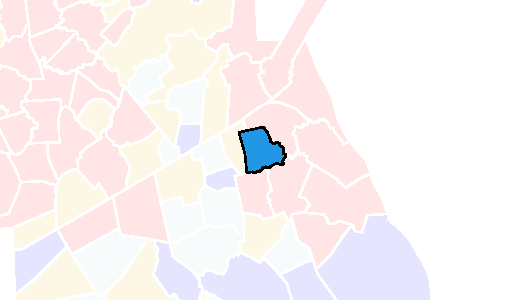
\includegraphics[keepaspectratio]{13_autocorrelation_files/figure-pdf/fig-map11-1.pdf}}

}

\caption{\label{fig-map11}County subdivision used to illustrate the
assessment of Local Moran's I significance. The observed Local Moran's I
statistic for this polygon is 0.85 and will be compared to values
generated from repeated permutations.}

\end{figure}%

Its Local Moran's \emph{I} statistic is 0.85. To assess its
significance, we perform a permutation test in which the income value of
the focal polygon is held constant while the income values of all other
polygons are randomly reassigned. Each permutation generates a new
\(I_i\) value based on a different neighborhood configuration. A few
example permutations are shown below.

\begin{figure}[H]

\centering{

\pandocbounded{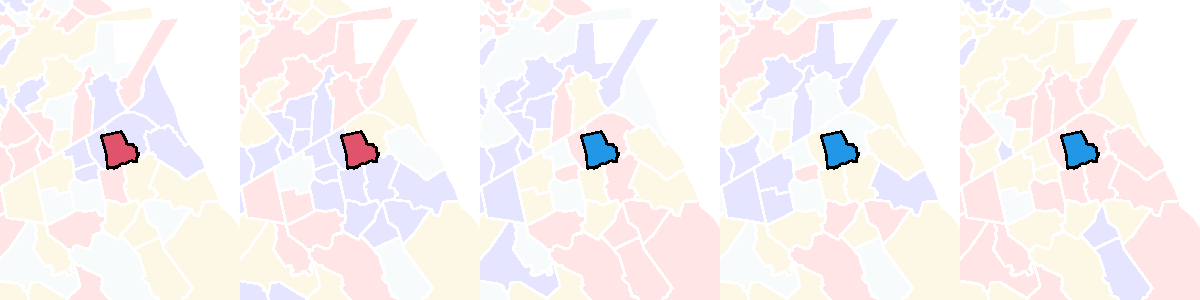
\includegraphics[keepaspectratio]{13_autocorrelation_files/figure-pdf/fig-map12-1.pdf}}

}

\caption{\label{fig-map12}Examples of Local Moran's I values generated
during the permutation procedure. The income value of the focal polygon
remains fixed while lagged income values are randomly reassigned,
producing different realizations of \(I_i\) under the null hypothesis of
spatial randomness.}

\end{figure}%

You'll note that even though the income value of the focal polygon
remains unchanged, its Local Moran's \emph{I} statistic varies because
the income values assigned to neighboring polygons change from one
permutation to the next.

Repeating this process many times generates a reference distribution of
\(I_i\) values under the null hypothesis that income values are randomly
distributed across Massachusetts. The observed \(I_i\) can then be
compared to this distribution to assess whether the local pattern is
more extreme than would be expected by chance. The resulting
distribution of \(I_i\) values for our example polygon is shown in the
following histogram.

\begin{figure}[H]

\centering{

\pandocbounded{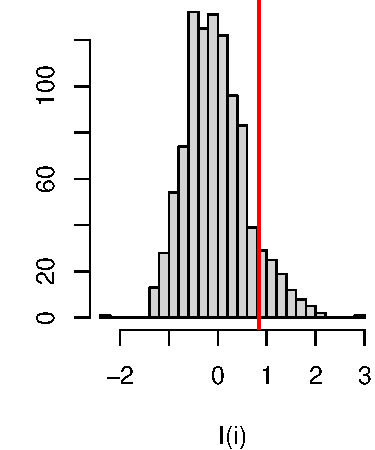
\includegraphics[keepaspectratio]{13_autocorrelation_files/figure-pdf/fig-map13-1.pdf}}

}

\caption{\label{fig-map13}Reference distribution of Local Moran's
\emph{I} values generated from repeated permutations. The red vertical
line marks the observed \(I_i\) value; its position relative to the
simulated distribution is used to assess statistical significance.}

\end{figure}%

About 9.3\% of the simulated values are more extreme than our observed
\(I_i\) giving us a permutation-based p-value of 0.09.

If we repeat this permutation test for every polygon in the dataset, we
can compute a permutation-based \emph{p}-value for each Local Moran's
\emph{I} statistic and map the results. These \emph{p}-values indicate
how unusual the observed local patterns are relative to what would be
expected under spatial randomness. Note that the mapped \emph{p}-values
represent the probability of obtaining an \(I_i\) value at least as
extreme as the observed value (equivalent to a \textbf{one-tailed
test}).

In the following map, lower \emph{p}-values identify locations where the
observed \(I_i\) values are less likely to have arisen by chance.

\begin{figure}[H]

\centering{

\pandocbounded{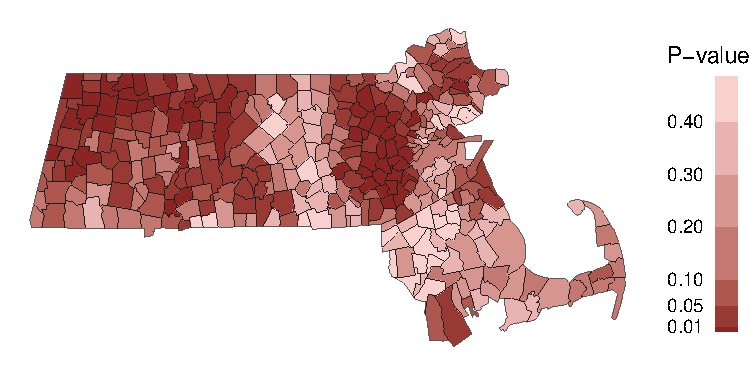
\includegraphics[keepaspectratio]{13_autocorrelation_files/figure-pdf/fig-map14-1.pdf}}

}

\caption{\label{fig-map14}Map of permutation-based \emph{p}-values for
Local Moran's \emph{I}. These values can be used to identify
statistically significant local clusters and spatial outliers by
applying a chosen significance threshold.}

\end{figure}%

The permutation-based \emph{p}-values can be used to filter the Local
Moran's \emph{I} classifications based on a chosen significance level.
For example, the following scatterplot and map show only those
high-high, low-low, high-low, and low-high relationships whose
permutation-based \emph{p}-value is 0.05 or less.

\begin{figure}[H]

\centering{

\pandocbounded{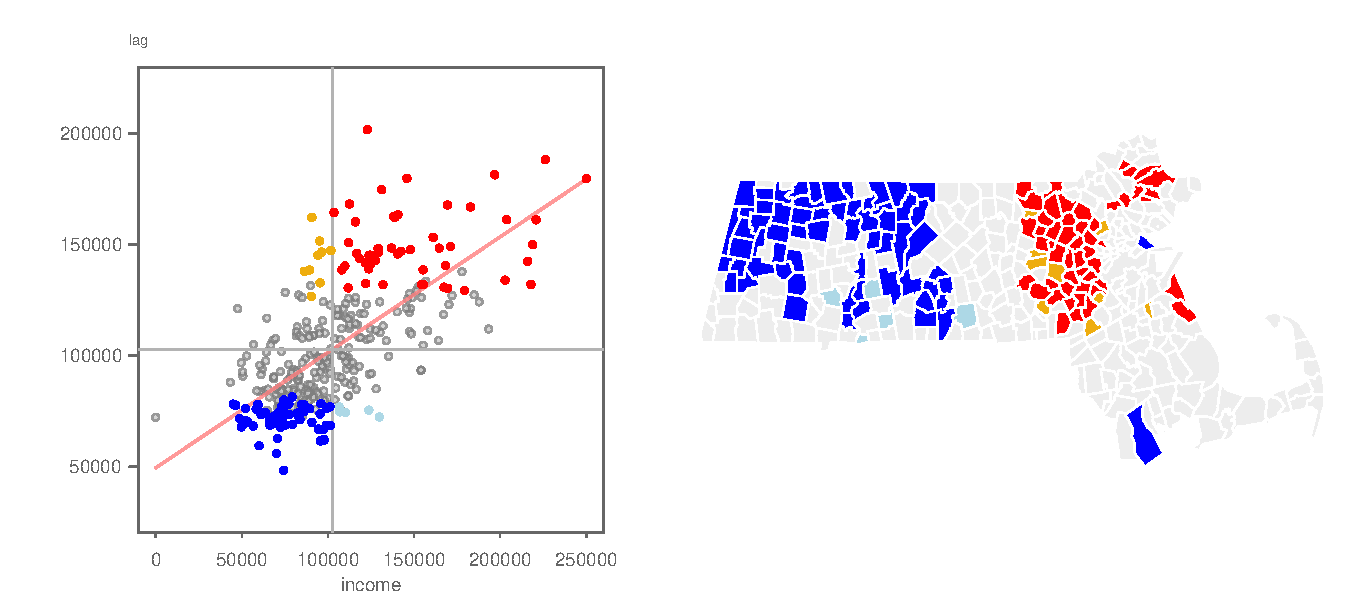
\includegraphics[keepaspectratio]{13_autocorrelation_files/figure-pdf/fig-map15-1.pdf}}

}

\caption{\label{fig-map15}Moran scatterplot classifications filtered
using a permutation-based significance threshold of \emph{p} \(\le\)
0.05. Only high-high, low-low, high-low, and low-high relationships
deemed statistically significant are shown.}

\end{figure}%

Note that statistical significance is not limited to high-high and
low-low clusters. High-low and low-high relationships can also be
statistically significant.

Figure~\ref{fig-map15} used a significance threshold of 0.05. Applying a
more stringent threshold of 0.01 retains only the strongest evidence of
local spatial association, as shown in the following figure.

\begin{figure}[H]

\centering{

\pandocbounded{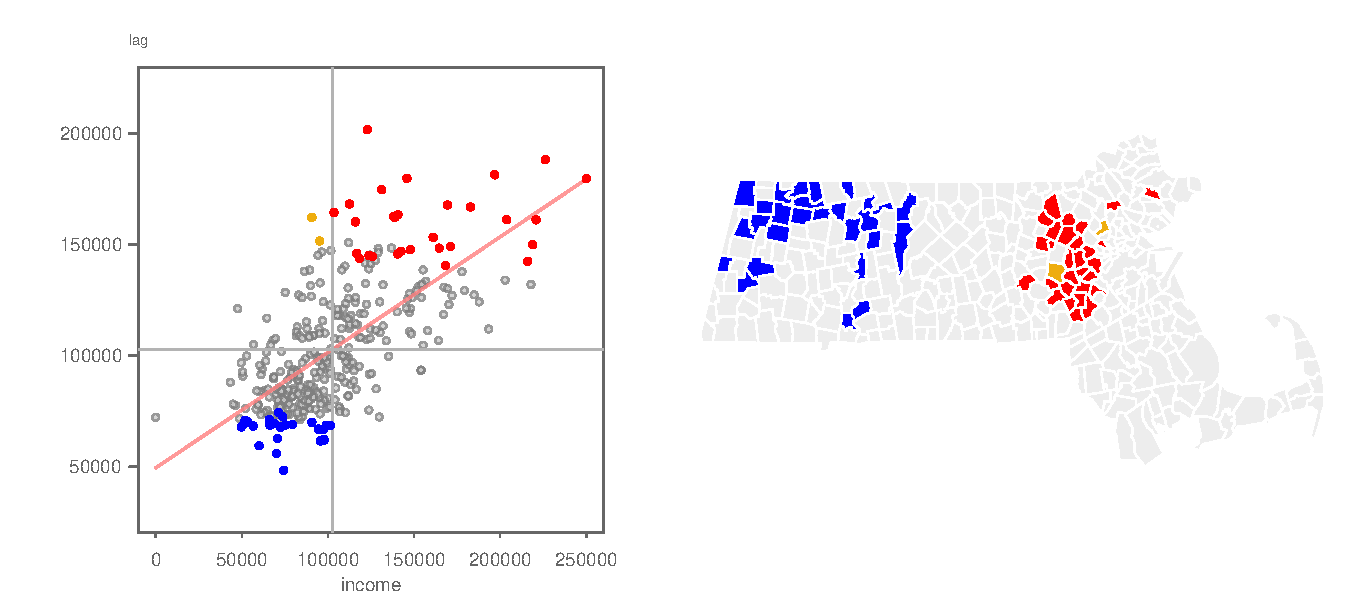
\includegraphics[keepaspectratio]{13_autocorrelation_files/figure-pdf/fig-map16-1.pdf}}

}

\caption{\label{fig-map16}Moran scatterplot classifications filtered
using a permutation-based significance threshold of \emph{p} \(\le\)
0.01. Only high-high, low-low, high-low, and low-high relationships
deemed statistically significant are shown.}

\end{figure}%

\subsection{Multiple Comparisons and False Discovery
Rate}\label{multiple-comparisons-and-false-discovery-rate}

While permutation tests are less sensitive to issues such as
non-normality and irregular spatial arrangements than many parametric
approaches, they are not immune to interpretational challenges. In
particular, when significance is assessed for every feature in a
dataset, some polygons may appear significant purely by chance. To
illustrate, suppose the income values were generated by a completely
random process. One possible realization might look like the following:

\begin{figure}[H]

\centering{

\pandocbounded{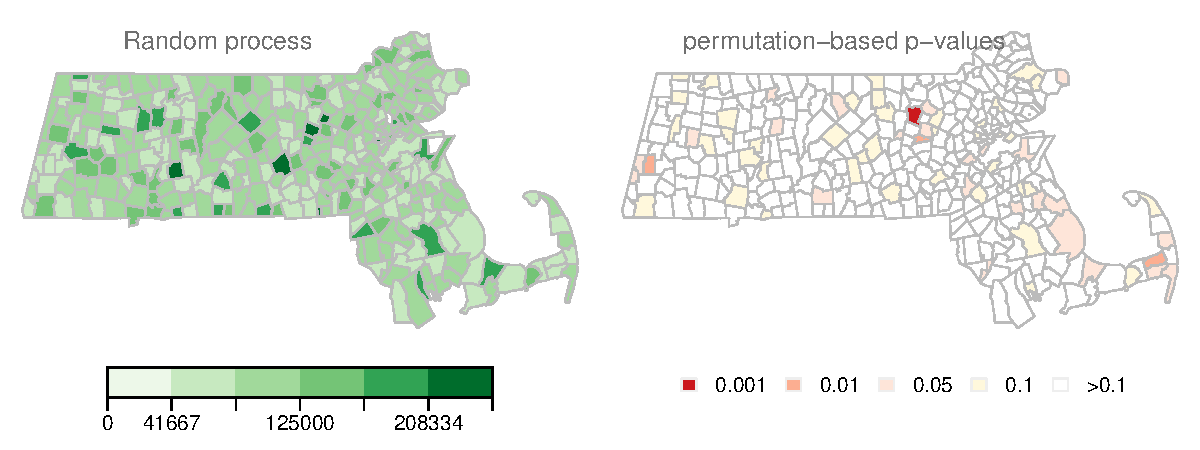
\includegraphics[keepaspectratio]{13_autocorrelation_files/figure-pdf/fig-map17-1.pdf}}

}

\caption{\label{fig-map17}Example realization of a random spatial
process. Although the income values were assigned randomly, several
polygons are associated with low permutation-based \emph{p}-values,
illustrating how statistically significant Local Moran's \emph{I} values
can arise by chance when many tests are performed.}

\end{figure}%

Notice that several polygons are associated with low permutation-based
p-values even though the underlying process is completely random. In
fact, one polygon has a permutation-based p-value of 0.001 or less. This
is not necessarily evidence of a meaningful spatial pattern. When
significance is assessed for many features simultaneously, some low
p-values are expected to occur by chance alone. In our example, 343
polygons result in 343 separate significance tests. This is analogous to
repeatedly drawing cards from a deck: the more opportunities you have to
draw the ace of spades, the greater the chance that you will eventually
draw one.

Another realization of a random spatial process is shown in the
following figure.

\begin{figure}[H]

\centering{

\pandocbounded{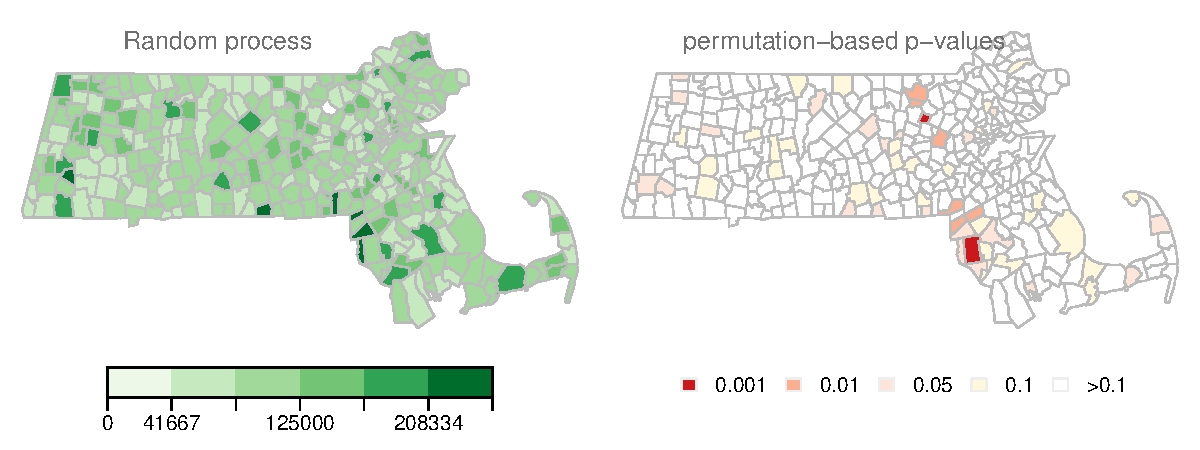
\includegraphics[keepaspectratio]{13_autocorrelation_files/figure-pdf/fig-map18-1.pdf}}

}

\caption{\label{fig-map18}A second realization of a random spatial
process. As in Figure~\ref{fig-map17}, several polygons exhibit low
permutation-based p-values despite the absence of true spatial
autocorrelation.}

\end{figure}%

Several polygons are associated with very low permutation-based p-values
(the smallest \emph{p}-value in this example is 0.0006). If these
results were viewed in isolation, one might conclude that several
polygons exhibit significant local spatial autocorrelation. However,
because the underlying process is completely random, these apparent
discoveries are false positives arising purely by chance, a classic
example of a \emph{Type I} error caused by multiple comparisons.

To further illustrate this issue, consider generating 200 independent
realizations of a random spatial process. For each realization, we
compute a permutation-based \emph{p}-value for every polygon, resulting
in a large number of simultaneous hypothesis tests and, consequently,
many opportunities for false positives. This generates 200×343 local
hypothesis tests and their associated \emph{p}-values. Even though all
realizations are random, approximately 10\% of the resulting
\emph{p}-values are 0.05 or less. This value should be interpreted as an
empirical outcome of this simulation rather than a theoretical
expectation, since Local Moran's \emph{I} tests are not independent and
neighboring polygons often share information through their spatial
relationships. The distribution of \emph{p}-values across all
simulations is shown in the following figure.

\begin{figure}[H]

\centering{

\pandocbounded{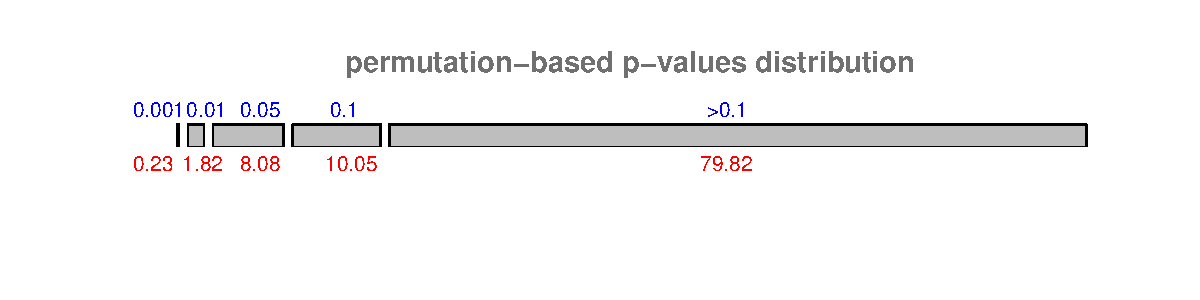
\includegraphics[keepaspectratio]{13_autocorrelation_files/figure-pdf/fig-map19-1.pdf}}

}

\caption{\label{fig-map19}Distribution of permutation-based
\emph{p}-values from 200 realizations of a random spatial process. Blue
labels denote the \emph{p}-value classes and red labels show the
percentage of observations in each class. Even under complete spatial
randomness, a substantial number of tests produce low p-values,
highlighting the accumulation of false positives when many hypothesis
tests are performed simultaneously.}

\end{figure}%

This problem is known in statistics as the \textbf{multiple comparison
problem}. Several approaches have been proposed to address it, each with
its own strengths and limitations. One of the most widely used solutions
is the \emph{False Discovery Rate} correction (FDR). Rather than
attempting to eliminate all false positives, the FDR approach seeks to
control the expected proportion of false positives among the set of
features declared significant.

There are several implementations of the FDR procedure. One common
approach begins by ranking the permutation-based \emph{p}-values, \(p\),
from smallest to largest and assigning a rank, \(i\), to each value.
Next, a reference value is computed for each rank as \(i(\alpha/n)\)
where \(\alpha\) is the desired significance level (0.05, for example)
and \(n\) is the total number of observations (e.g.~polygons) for which
a permutation-based \emph{p}-value has been computed (343 in our working
example). All \emph{p}-values that satisfy \(p_i \le i(\alpha/n)\) are
considered significant at the chosen \(\alpha\) level.

Applying the FDR correction to the permutation-based significance
threshold of 0.05 produces a more conservative cluster map than the one
shown in Figure~\ref{fig-map15}, reducing the likelihood of false
positives arising from multiple comparisons.

\begin{figure}[H]

\centering{

\pandocbounded{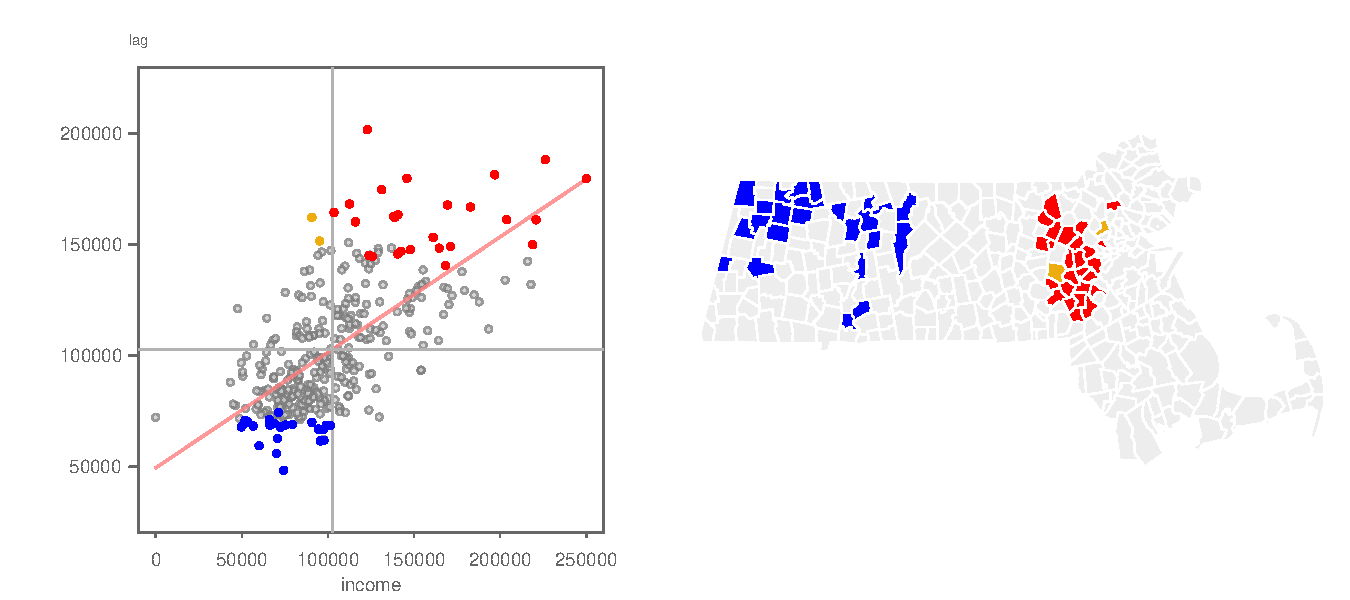
\includegraphics[keepaspectratio]{13_autocorrelation_files/figure-pdf/fig-map20-1.pdf}}

}

\caption{\label{fig-map20}Local Moran's I classifications deemed
significant at \(\alpha = 0.05\) after applying the False Discovery Rate
(FDR) correction. Compared to the uncorrected results, fewer polygons
are identified as significant, reducing the likelihood of false
positives.}

\end{figure}%

Applying the FDR correction to a significance threshold of 0.01 yields
an even more conservative set of clusters than those shown in
Figure~\ref{fig-map16}. By accounting for the large number of
simultaneous hypothesis tests, the correction retains only the strongest
evidence of local spatial association, as shown in the following figure.

\begin{figure}[H]

\centering{

\pandocbounded{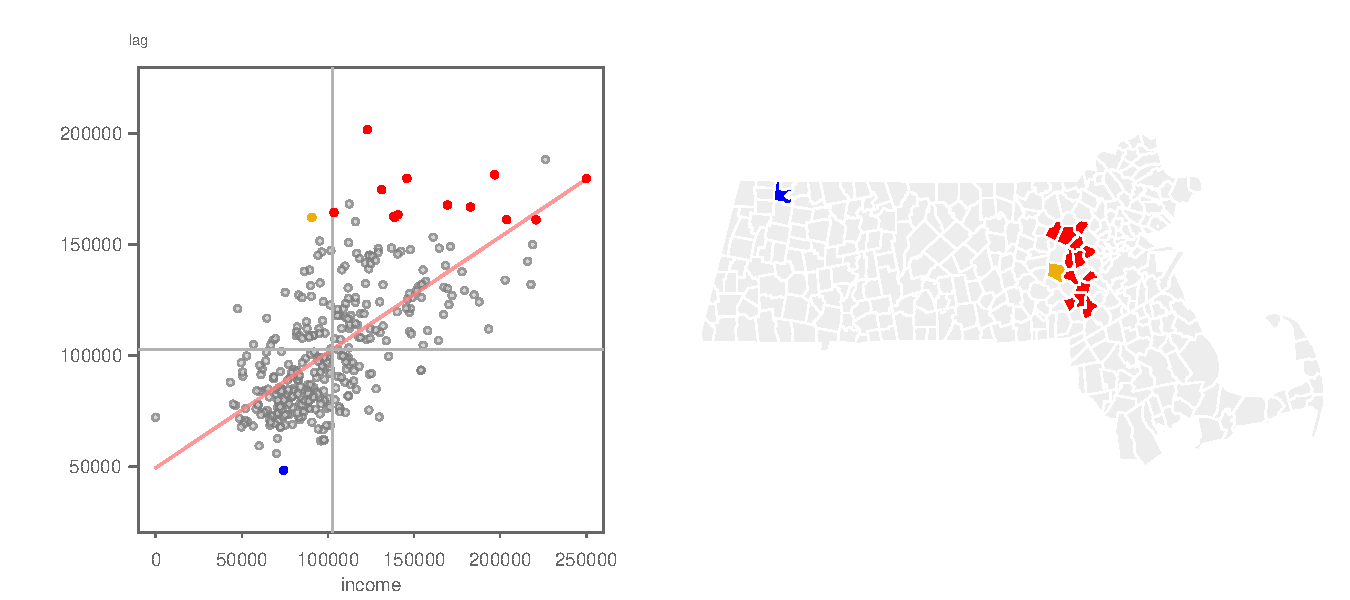
\includegraphics[keepaspectratio]{13_autocorrelation_files/figure-pdf/fig-map21-1.pdf}}

}

\caption{\label{fig-map21}Local Moran's I classifications deemed
significant at \(\alpha = 0.01\) after applying the False Discovery Rate
(FDR) correction. The more stringent significance threshold retains only
the strongest local spatial relationships.}

\end{figure}%

It is important to recognize that there is no universally accepted
solution to the multiple-comparison problem. Spatial data introduce
additional complications because neighboring features often share
information. For example, the same polygon may contribute to the Local
Moran's I calculations of several neighboring polygons, violating the
assumption that individual tests are independent. These and other
sources of dependence make inferential interpretation in a spatial
context particularly challenging. As a result, significance maps derived
from Local Moran's I analyses should be interpreted with caution.

\section{Moran's I equation
explained}\label{morans-i-equation-explained}

The Moran's \emph{I} statistic can be expressed in several
mathematically equivalent forms, each offering different insights into
its structure and interpretation. One commonly used formulation is:

\[
I = \frac{N}{\sum\limits_i (X_i-\bar X)^2} 
    \frac{\sum\limits_i \sum\limits_j w_{ij}(X_i-\bar X)(X_j-\bar X)}{\sum\limits_i \sum\limits_j w_{ij}} \tag{1}
\]

Here, \(N\) is the total number of spatial units, \(X_i\) and \(X_j\)
are the attribute values at locations \(i\) and \(j\), \(\bar{X}\) is
the mean of \(X\), and \(w_{ij}\) is the spatial weight between
locations \(i\) and \(j\)--typically defined by contiguity, distance, or
other spatial relationships.

There are a few key components of Equation (1) worth highlighting.
First, you'll note the standardization of both sets of values by the
subtraction of each value in \(X_i\) or \(X_j\) by the mean of \(X\).
This highlights the fact that we are seeking to compare the deviation of
each value from an overall mean and not the deviation of their absolute
values.

Second, you'll note an inverted variance term on the left-hand side of
equation (1): this is a measure of spread. You might recall from an
introductory statistics course that the variance can be computed as:

\[
s^2 = \frac{\sum\limits_i (X_i-\bar X)^2}{N}\tag{2}
\] Note that a more common measure of variance, the sample variance,
where one divides the above numerator by \((n-1)\) can also be adopted
in the Moran's \emph{I} calculation.

Equation (1) is thus dividing the large fraction on the right-hand side
by the variance. Standardization causes Moran's I to behave similarly to
a correlation coefficient with values typically falling near the range
{[}-1,1{]}. However, the exact bounds depend on the spatial weights
matrix and may extend beyond this interval. We can re-write the Moran's
I equation by plugging in \(s^2\) as follows:

\[
I = \frac{\sum\limits_i \sum\limits_j w_{ij}\frac{(X_i-\bar X)}{s}\frac{(X_j-\bar X)}{s}}{\sum\limits_i \sum\limits_j w_{ij}} \tag{3}
\] Note that here \(s\times s = s^2\). You might recognize the numerator
as a sum of the product of standardized \emph{z}-values between
neighboring features. If we let \(z_i = \frac{(X_i-\bar X)}{s}\) and
\(z_j = \frac{(X_j-\bar X)}{s}\), The Moran's I equation can be reduced
to:

\[
I = \frac{\sum\limits_i \sum\limits_j w_{ij}(z_i\ z_j)}{\sum\limits_i \sum\limits_j w_{ij}} \tag{4}
\]

Recall that we are comparing a variable \(X\) at location \(i\) to the
values observed at neighboring locations \(j\). If we define,

\[
y_i = \sum\limits_j w_{ij} z_j
\] then \(y_i\) represents a spatially lagged value. When the weights
matrix is \emph{row-standardized}, the weights associated with each
feature sum to one and \(y_i\) becomes the weighted average of the
neighboring standardized values.

the Moran's I coefficient can be rewritten as:

\[
I = \frac{\sum\limits_i z_i y_i}{\sum\limits_i \sum\limits_j w_{ij}}  \tag{5}
\]

Under row-standardized weights, \(y_i\) is the average z-value making
the product \(z_i y_i\) a local measure of \emph{spatial association}.

The product \(z_iy_i\) is a local measure of spatial autocorrelation,
\(I_i\). If we \emph{don't} summarize across all locations \(i\), under
row-standardized weights, Local Moran's I can be expressed as:

\[
I_i = z_iy_i  \tag{6}
\] The global Moran's \emph{I} statistic, \(I\), is thus the average of
all \(I_i\) values.

\[
I = \frac{\sum\limits_i I_i}{\sum\limits_i \sum\limits_j w_{ij}}  \tag{5}
\]

Let's explore elements of the Moran's \emph{I} equation using the
following sample dataset.

\begin{figure}[H]

\centering{

\pandocbounded{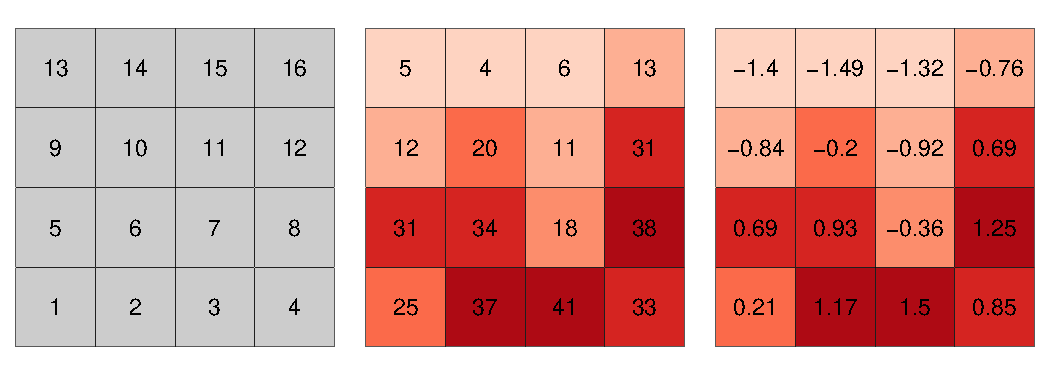
\includegraphics[keepaspectratio]{13_autocorrelation_files/figure-pdf/fig-map22-1.pdf}}

}

\caption{\label{fig-map22}Simulated spatial dataset used to demonstrate
the components of the Moran's I equation. The left panel displays cell
identifiers, the middle panel shows the observed values, and the right
panel shows the standardized (\emph{z}) values derived from those
observations.}

\end{figure}%

The first step in the computation of a Moran's \emph{I} index is the
generation of a spatial weights matrix. The weights can take on many
different values. For example, one could assign a value of \texttt{1} to
a neighboring cell as shown in the following matrix.

\begin{table}

\caption{\label{tbl-map23}Binary spatial weights matrix used in the
calculation of Moran's I. Rows correspond to focal locations (\(i\)) and
columns correspond to neighboring locations (\(j\)). Neighbor pairs are
assigned a weight of 1, while non-neighbor pairs are assigned a weight
of 0.}

\centering{

\pandocbounded{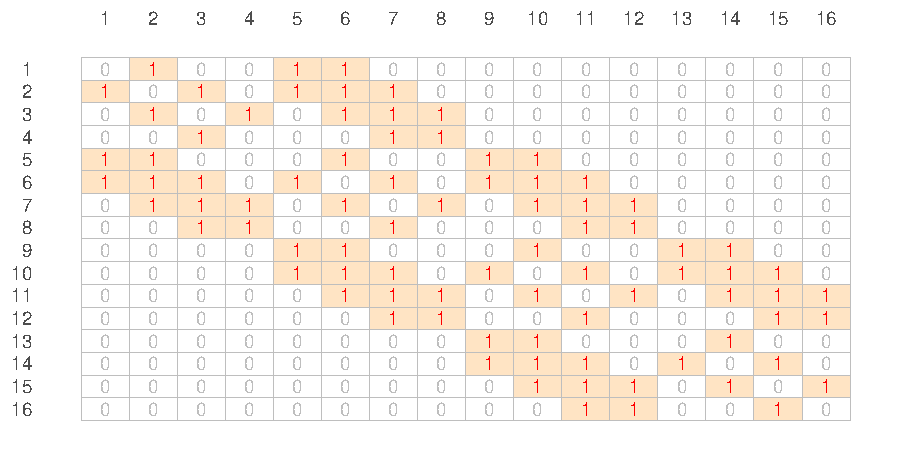
\includegraphics[keepaspectratio]{13_autocorrelation_files/figure-pdf/tbl-map23-1.pdf}}

}

\end{table}%

For example, cell ID \texttt{1} (whose value is 25 and whose
standardized value, \(z_1\), is 0.21) has for neighbors cells
\texttt{2}, \texttt{5} and \texttt{6}. Computationally (working with the
standardized values), this gives us a summarized lagged value,
\(y_1(lag)\) of:

\begin{align*}
y_1 =  \sum\limits_j w_{1j} z_j {}={} & (0)(0.21)+(1)(1.17)+(0)(1.5)+ ... + \\
                                      & (1)(0.69)+(1)(0.93)+(0)(-0.36)+...+ \\
                                      & (0)(-0.76) = 2.79
\end{align*}                                  

Computing the spatially lagged values for the other 15 cells generates
the following scatterplot:

\begin{figure}[H]

\centering{

\pandocbounded{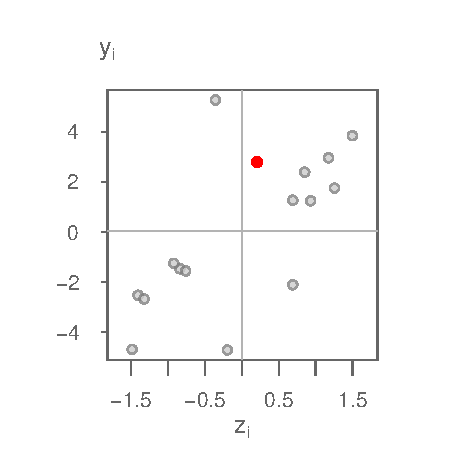
\includegraphics[keepaspectratio]{13_autocorrelation_files/figure-pdf/fig-map24-1.pdf}}

}

\caption{\label{fig-map24}Moran scatterplot based on binary spatial
weights. The red point identifies cell 1. Note that the lagged values
(\(y_i\)) span a much larger range than the original standardized values
(\(z_i\)) because each neighboring value contributes equally and the
weights are not standardized.}

\end{figure}%

You'll note that the range of lagged values along the \(y\)-axis is much
greater than that of the original standardized values along the
\(x\)-axis. This is not necessarily problematic because Moran's I is
computed from standardized values. However, the differing scales reveal
a limitation of binary weights: features with many neighbors tend to
have larger lagged values than features with fewer neighbors simply
because more neighboring values contribute to the sum. For example,
feature ID 12, which has five neighbors, will tend to have a larger
lagged value than feature ID 1, which has only three neighbors. This
motivates the use of row-standardized weights where the weights
associated with each feature sum to one.

A more natural weight is one where the values are standardized across
each row of the weights matrix such that the weights across each row sum
to one. For example:

\begin{table}

\caption{\label{tbl-map25}Row-standardized spatial weights matrix used
in the computation of Moran's I. Standardizing each row removes the
influence of differing numbers of neighbors by ensuring that all rows
sum to one.}

\centering{

\pandocbounded{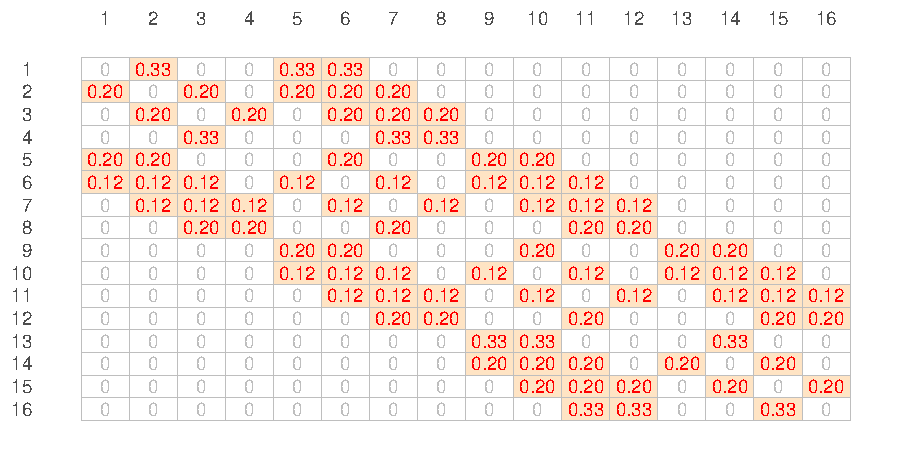
\includegraphics[keepaspectratio]{13_autocorrelation_files/figure-pdf/tbl-map25-1.pdf}}

}

\end{table}%

The spatially lagged value for cell ID \texttt{1} is thus computed as:

\begin{align*}
y_1 =  \sum\limits_j w_{1j} z_j {}={} & (0)(0.21)+(0.333)(1.17)+(0)(1.5)+...+ \\
                                      & (0.333)(0.69)+(0.333)(0.93)+(0)(-0.36)+...+ \\
                                      & (0)(-0.76) = 0.93
\end{align*}

Multiplying each neighbor by the standardized weight, then summing these
values, is simply computing the neighbor's mean value.

Using the standardized weights generates the following scatter plot.
Plot on the left shows the raw values on the \emph{x} and \emph{y} axes;
plot on the right shows the standardized values \(z_i\) and
\(y_i = \sum\limits_j w_{ij} z_j\). You'll note that the shape of the
point cloud is the same in both plots given that the axes on the left
plot are scaled such as to match the standardized scales in both axes.

\begin{figure}[H]

\centering{

\pandocbounded{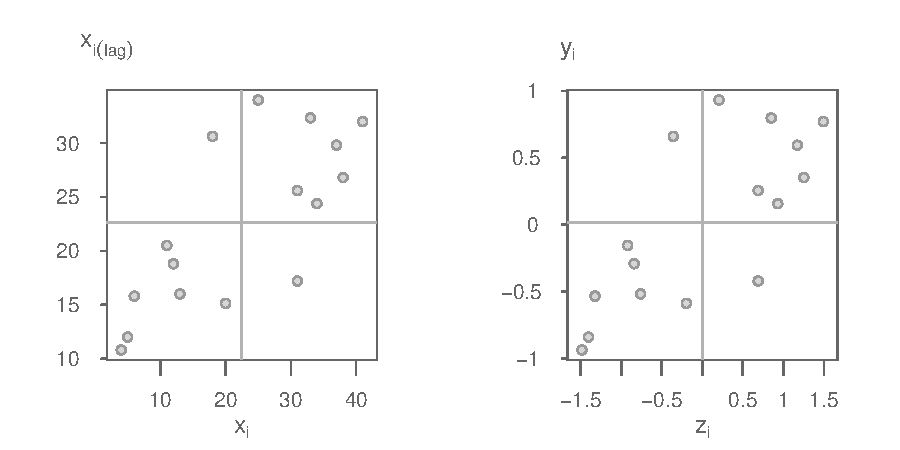
\includegraphics[keepaspectratio]{13_autocorrelation_files/figure-pdf/fig-map26-1.pdf}}

}

\caption{\label{fig-map26}Moran scatterplots generated using
row-standardized weights. The left plot uses the original values and
their lagged counterparts, while the right plot uses standardized values
(\(z_i\) and \(y_i\)). Row standardization causes each lagged value to
represent a weighted average of neighboring values.}

\end{figure}%

Note the difference in the point cloud pattern from that generated using
the binary weights (Figure~\ref{fig-map24}). Under row-standardization,
the lagged values represent weighted averages of neighboring values
rather than simple sums, reducing the influence of varying neighbor
counts on the calculation of \(y_i\). Other weighting schemes can also
be used, including inverse-distance and \emph{k}-nearest-neighbor
weights. However, most software implementations of Moran's I adopt
row-standardized weights because they facilitate interpretation and
reduce the influence of differing numbers of neighbors.

\subsection{Local Moran's I}\label{local-morans-i-1}

Once a spatial weight is chosen, and both \(z_i\) and \(y_i\) are
computed, we can compute the \(z_iy_i\) product for all locations of
\(i\) thus giving us a measure of the local Moran's I statistic. Taking
feature ID of \texttt{1} in our example, we compute
\(I_1(lag) = 0.21 \times 0.93 = 0.19\). Computing \(I_i\) for all cells
gives us the following plot.

\begin{figure}[H]

\centering{

\pandocbounded{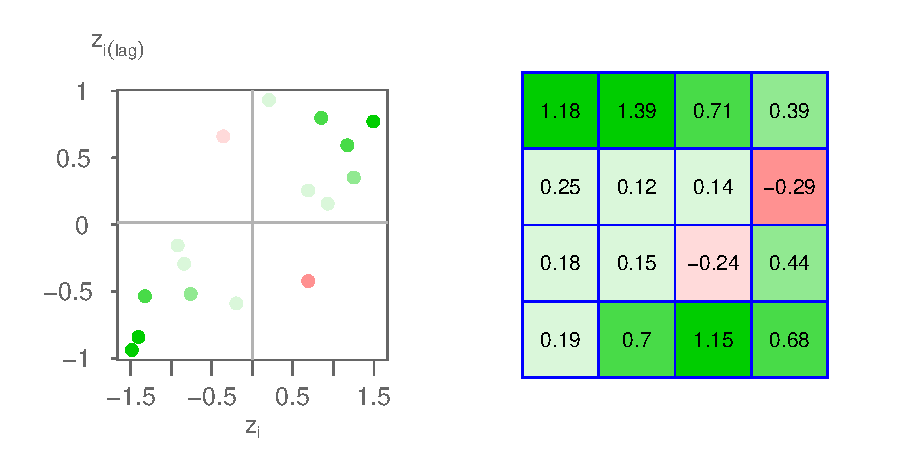
\includegraphics[keepaspectratio]{13_autocorrelation_files/figure-pdf/fig-map27-1.pdf}}

}

\caption{\label{fig-map27}Local Moran's \emph{I} values for the
simulated dataset. Positive values indicate locations surrounded by
neighbors with similar standardized values, whereas negative values
indicate locations surrounded by dissimilar neighboring values. The
scatterplot (left) and map (right) show the same \(I_i\) values.}

\end{figure}%

Here, we are adopting a different color scheme from that used earlier.
Green colors highlight features whose values are surrounded by similar
values. These can be either positive values surrounded by standardized
values that tend to be positive or negative values surrounded by values
that tend to be negative. In both cases, the calculated \(I_i\) will be
positive. Red colors highlight features whose values are surrounded by
dissimilar values. These can be either negative values surrounded by
values that tend to be positive or positive values surrounded by values
that tend to be negative. In both cases, the calculated \(I_i\) will be
negative. In our example, two features have a negative Moran's \emph{I}
coefficient: cell IDs \texttt{7} and \texttt{12}.

\subsection{Global Moran's I}\label{global-morans-i-1}

The Global Moran's \emph{I} coefficient, \(I\) can be viewed as a
summary of the local Moran's \emph{I} coefficients. Using
row-standardized weights, the global Moran's I statistic can be
expressed as a weighted average of the local Moran's I statistics.

\[
\begin{pmatrix}
\frac{0.19+0.7+1.15+0.68+0.18+0.15+-0.24+0.44+0.25+0.12+0.14+-0.29+1.18+1.39+0.71+0.39}{\sum\limits_i\sum\limits_j w_{ij}} = 0.446
\end{pmatrix}
\] In this example, \(\sum\limits_i \sum\limits_j w_{ij}\) is the sum of
all 256 values in Table~\ref{tbl-map25} which, using standardized
weights, sums to 16.

\(I\) is thus the slope that best fits the data in the Moran
scatterplot. This can be plotted using either the standardized values or
the raw values.

\begin{figure}[H]

\centering{

\pandocbounded{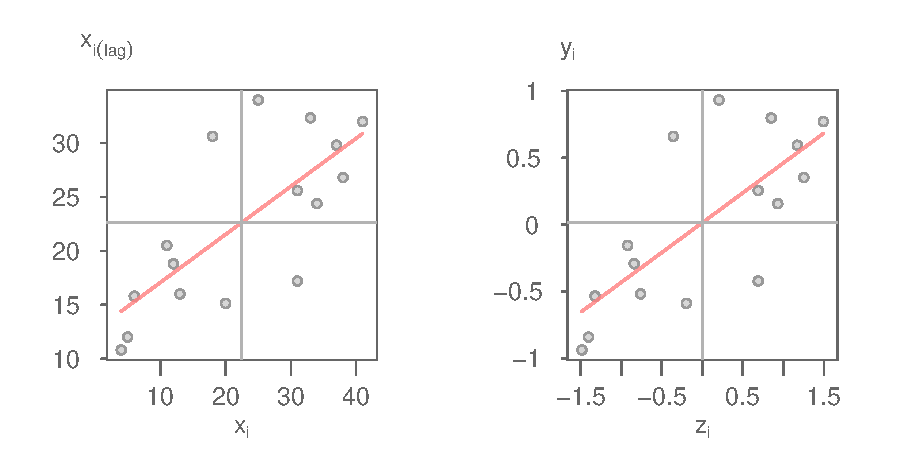
\includegraphics[keepaspectratio]{13_autocorrelation_files/figure-pdf/fig-map28-1.pdf}}

}

\caption{\label{fig-map28}Moran scatterplot showing the fitted Global
Moran's \emph{I} slope (red line). A positive slope indicates that
locations with above-average values tend to be surrounded by neighbors
whose values are also above average, while locations with below-average
values tend to be surrounded by neighbors whose values are also below
average.}

\end{figure}%

\section{Summary}\label{summary-11}

This chapter introduced spatial autocorrelation as a second-order
property describing how values at one location relate to values at
nearby locations. Using Moran's \emph{I} as a central measure, we
explored how spatial relationships can be quantified, tested, and
interpreted across different spatial scales.

\begin{itemize}
\tightlist
\item
  \textbf{Spatial autocorrelation} measures the degree to which nearby
  locations have similar or dissimilar attribute values.
\item
  \textbf{Global Moran's \emph{I}} provides a summary measure of spatial
  autocorrelation for an entire study area and can be interpreted as the
  relationship between a variable and its spatially lagged counterpart.
\item
  The computation of Moran's \emph{I} depends on a \textbf{spatial
  weights matrix}, which defines neighborhood relationships based on
  contiguity, distance, nearest neighbors, or other criteria.
\item
  \textbf{Permutation tests} provide a flexible, non-parametric approach
  for assessing whether observed Moran's \emph{I} values are more
  extreme than would be expected under spatial randomness.
\item
  Spatial autocorrelation can vary with \textbf{distance}, making it
  possible to explore how spatial relationships strengthen, weaken, or
  change sign across spatial scales.
\item
  \textbf{Local Moran's \emph{I}} decomposes the global statistic into
  feature-level measures, allowing local clusters and spatial outliers
  to be identified.
\item
  Permutation-based significance tests can be applied to Local Moran's
  \emph{I} statistics to assess whether local patterns are unlikely to
  have occurred by chance.
\item
  Because Local Moran's \emph{I} involves many simultaneous hypothesis
  tests, results are susceptible to the \textbf{multiple-comparison
  problem}, increasing the likelihood of false positives.
\item
  Procedures such as the \textbf{False Discovery Rate (FDR)} correction
  can help control the expected proportion of false discoveries,
  although no single correction completely resolves the challenges of
  spatial inference.
\item
  Moran's \emph{I} can be viewed as a spatially weighted measure of
  association, providing a bridge between descriptive analysis of
  spatial patterns and formal statistical inference.
\end{itemize}

\chapter{First-Order Point Pattern
Analysis}\label{first-order-point-pattern-analysis}

\section{Introduction}\label{introduction-13}

In spatial \textbf{point pattern} analysis, \textbf{first-order effects}
refer to variations in the intensity of points across a study area due
to external factors. These effects describe how the likelihood of
observing a point changes from one location to another, independent of
the presence or absence of other points. For example, oak trees may be
more densely distributed in areas with favorable soil conditions, or
retail stores may cluster in regions with higher population density. In
both cases, the spatial variation is driven by underlying environmental
or socioeconomic covariates rather than interactions between the points
themselves.

This concept is analogous to the spatial trend models introduced in
Chapter 12 for continuous fields. There, we modeled how attribute values
varied as a function of location. Here, we focus on how the intensity of
a point process varies across space. In both cases, the objective is to
characterize first-order effects before investigating potential
second-order effects.

This chapter focuses on techniques for detecting and modeling these
first-order effects. We begin with simple descriptive tools such as
\textbf{global} and \textbf{local} density measures, then move to more
refined methods such as kernel density estimation and covariate-adjusted
intensity modeling. Finally, we introduce statistical models, such as
the Poisson point process model, that allow us to formally test
hypotheses about how external variables influence point intensity. By
characterizing and accounting for first-order effects, we lay the
groundwork for the second-order analyses presented in the next chapter
where the focus shifts from spatial variation in intensity to
interactions among points.

\section{Understanding Intensity and Density in Point
Patterns}\label{understanding-intensity-and-density-in-point-patterns}

In point pattern analysis, the terms \textbf{intensity} and
\textbf{density} are closely related but conceptually distinct.
Understanding the difference is important when interpreting spatial
patterns and building models.

\begin{itemize}
\item
  \textbf{Density} refers to the \textbf{observed number of points per
  unit area} in a dataset. It's a descriptive statistic: what we
  actually count from the data. For example, if there are 31 trees in a
  100 square meter plot, the density is 0.31 trees per square meter.
\item
  \textbf{Intensity}, on the other hand, refers to the
  \textbf{underlying rate or likelihood} that a point occurs at a
  location. It's a property of the \textbf{process} that generated the
  pattern, not simply the observed pattern itself. Intensity is often
  denoted by the symbol \(\lambda\) and can vary across space. When we
  estimate intensity from observed data, we use \(\widehat{\lambda}\) to
  indicate that it's an approximation.
\end{itemize}

Think of it this way: density is \emph{what we observe}, intensity is
\emph{what we infer}. If the intensity is constant across the study
area, the process is said to be \textbf{homogeneous}. If intensity
varies across space, the process is \textbf{inhomogeneous}.

Spatial variation in intensity is the point-pattern analogue of a
spatial trend in continuous field data. In both cases, the goal is to
characterize first-order effects before examining possible second-order
interactions. We therefore need tools that can model how intensity
changes with location or covariates.

\section{Global density}\label{global-density}

A basic estimate of a point pattern's \emph{intensity},
\(\widehat{\lambda}\), is its global density: the average number of
observed points per unit area across the entire study region. While
density is an observed quantity and intensity is a property of the
underlying process, the global density provides a simple estimate of
intensity under the assumption that the process is homogeneous. It is
computed as the ratio of the total number of observed points, \(n\), to
the surface area of the study region, \(a\):

\begin{equation}
\widehat{\lambda} = \frac{n}{a}
\label{eq:global-density}
\end{equation}

This estimate assumes that the underlying point process is homogeneous,
meaning the intensity is constant throughout the region.

\begin{figure}[H]

\centering{

\pandocbounded{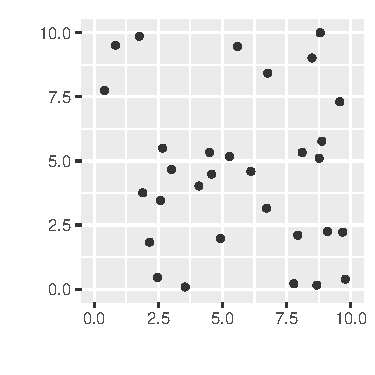
\includegraphics[keepaspectratio]{14_ppa_1st_files/figure-pdf/fig-gobal_dens-1.pdf}}

}

\caption{\label{fig-gobal_dens}Example of a point pattern containing 31
observed points within a study area of 100 square units. Under the
assumption of a homogeneous point process, the global intensity estimate
\(\widehat{\lambda}\) is 31/100 = 0.31 points per unit area.}

\end{figure}%

While useful as a summary statistic, global density provides only a
single value for the entire study area and can mask important spatial
variation. To investigate whether intensity changes across space, we
need local density measures.

\section{Local density}\label{local-density}

A point pattern's density can vary across space, and measuring it at
different locations allows us to assess whether the underlying process's
local intensity, \(\widehat{\lambda}_i\), is spatially uniform or not.
Spatial variation in intensity is a hallmark of a \textbf{first-order
effect}, where external factors influence the likelihood of observing
points in some parts of the study area more than others. Estimating
local density therefore provides a way to explore how intensity changes
across space and whether the assumption of a homogeneous process is
reasonable.

Identifying non-uniform intensity is important because many second-order
analyses (covered in the next chapter) assume \textbf{stationarity}: the
assumption that the underlying process generating the points has a
constant intensity across the study area.

As with spatial trends in continuous fields, variation in intensity can
create the \emph{appearance} of clustering even when no interaction
exists among points.

Local density methods do not directly explain why intensity varies, but
they can help identify areas where the underlying process may be
stronger or weaker, thereby guiding subsequent modeling efforts.

Several techniques are available for estimating local density. In this
chapter, we focus on two widely used methods: \emph{quadrat density},
which divides the study area into discrete subregions, and \emph{kernel
density}, which uses a moving window to produce a smooth surface of
estimated intensity.

\subsection{Quadrat density}\label{quadrat-density}

One simple way to estimate local density is to divide the study area
into smaller regions and compute a separate density value for each
region. \textbf{Quadrat density} analysis involves dividing the study
area into sub-regions called quadrats. For each quadrat, the
\textbf{local density} is computed by dividing the number of points
within the quadrat by its area. This provides a spatially localized
estimate of point intensity. In effect, quadrat analysis replaces the
single global density value introduced earlier with a collection of
local density estimates distributed across the study area.

This method assumes that the intensity of the point process is roughly
constant within each quadrat, which may not hold if quadrats are too
large or poorly aligned with underlying spatial variation.

Quadrats can take various shapes such as hexagons and triangles. The
following example divides the study area into four equally sized square
quadrats and computes a local density value for each.

\begin{figure}[H]

\centering{

\pandocbounded{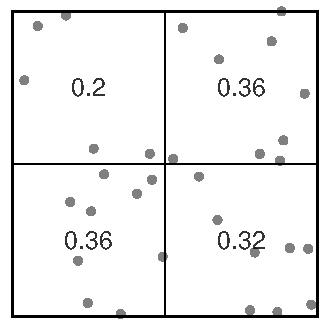
\includegraphics[keepaspectratio]{14_ppa_1st_files/figure-pdf/fig-quad01-1.pdf}}

}

\caption{\label{fig-quad01}Example of a quadrat density analysis. The
study area is divided into four equally sized quadrats, and a local
density value is computed for each by dividing the number of points
within the quadrat by its area.}

\end{figure}%

The choice of quadrat size, number, and shape can influence the measure
of local density and must be chosen with care. If very small quadrat
sizes are used, you risk having many empty quadrats which may prove
uninformative. If very large quadrat sizes are used, you risk missing
subtle changes in spatial density distributions such as an east-west
gradient in density values.

Instead of dividing the study area into uniform shapes, quadrats can
also be defined based on an underlying \textbf{covariate}: a spatial
variable believed to influence point intensity (e.g., elevation, land
cover, or population density). For example, if it's believed that the
underlying point pattern process is driven by elevation, quadrats can be
defined by sub-regions such as different ranges of elevation values
(labeled 1 through 4 on the right-hand plot in the following example).
This can result in quadrats with non-uniform shape and area. This idea
moves us from describing where points occur to exploring whether
intensity may be related to an underlying environmental variable.

\begin{quote}
Converting a continuous field into discretized areas is sometimes
referred to as \textbf{tessellation}. The end product is a
\textbf{tessellated surface}.
\end{quote}

\begin{figure}[H]

\centering{

\pandocbounded{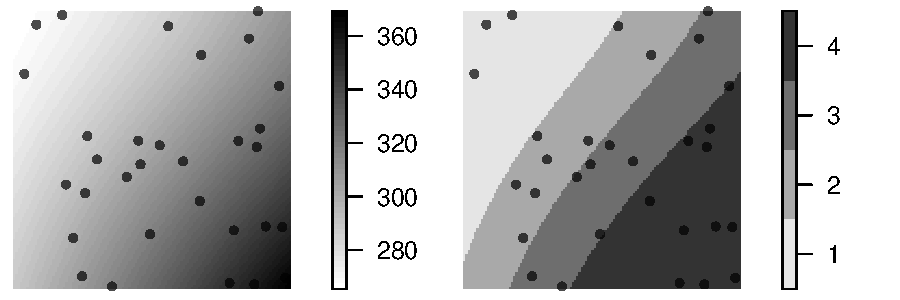
\includegraphics[keepaspectratio]{14_ppa_1st_files/figure-pdf/fig-quad02-1.pdf}}

}

\caption{\label{fig-quad02}Example of covariate-based quadrats. The
elevation surface (left) is divided into four elevation classes (right),
creating a tessellated surface that can be used to examine how point
density varies with elevation.}

\end{figure}%

If the local intensity changes across the tessellated covariate, then
there is evidence of a dependence between the process that generated the
point pattern and the covariate. In our example, sub-regions 1 through 4
have surface areas of 23.54, 25.2, 25.21, 26.06 map units respectively.
To compute these regions' point densities, we simply divide the number
of points by the respective area values. The resulting point counts and
density estimates are shown below.

\begin{figure}[H]

\centering{

\pandocbounded{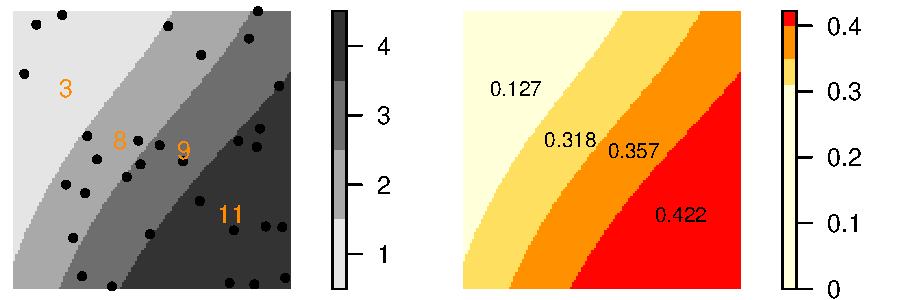
\includegraphics[keepaspectratio]{14_ppa_1st_files/figure-pdf/fig-quad03-1.pdf}}

}

\caption{\label{fig-quad03}Density estimates for elevation-defined
subregions. The left panel shows the number of observed points within
each elevation class, while the right panel shows the corresponding
densities after accounting for differences in subregion area.}

\end{figure}%

We can plot the relationship between point density and elevation region
to help assess whether intensity varies systematically with elevation.

\begin{figure}[H]

\centering{

\pandocbounded{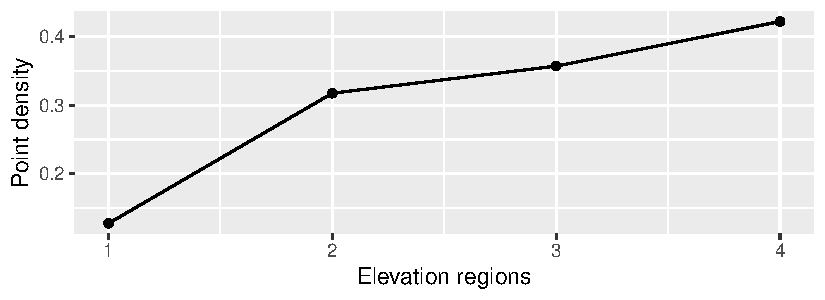
\includegraphics[keepaspectratio]{14_ppa_1st_files/figure-pdf/fig-quad04-1.pdf}}

}

\caption{\label{fig-quad04}Relationship between point density and
elevation class. The increasing density values suggest that point
intensity may be associated with elevation, although the quadrat
approach alone cannot determine whether this relationship is
statistically significant.}

\end{figure}%

It's important to note that how one \emph{chooses} to tessellate a
surface can have an influence on the resulting density distribution. For
example, dividing the elevation into seven sub-regions produces the
following density values.

\begin{figure}[H]

\centering{

\pandocbounded{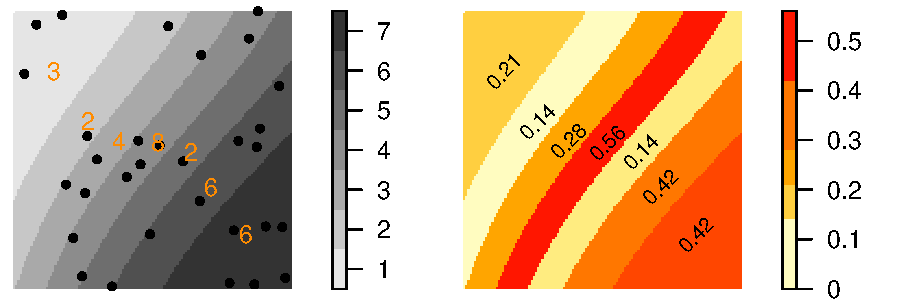
\includegraphics[keepaspectratio]{14_ppa_1st_files/figure-pdf/fig-quad05-1.pdf}}

}

\caption{\label{fig-quad05}Local density estimates computed using a
different tessellation of the elevation surface. Changes in the density
values reflect the influence of zone definition on quadrat-based
analyses, an example of the Modifiable Areal Unit Problem (MAUP).}

\end{figure}%

While the higher density observed in the western portion of the study
area remains evident, the density pattern elsewhere depends on how the
elevation surface is partitioned.

The quadrat analysis approach has advantages: it is straightforward to
compute and easy to interpret. However, it is susceptible to the
\hyperref[maup]{modifiable areal unit problem} (MAUP) as illustrated by
the previous two examples.

Quadrat density is most useful when the study area can be meaningfully
divided into regions of interest, or when a covariate provides a natural
way to segment space. However, quadrat methods can struggle to capture
gradual or continuous changes in intensity across space. This limitation
motivates the kernel density methods introduced next.

\subsection{Kernel density}\label{kernel-density}

While quadrat density provides localized estimates of intensity, it
imposes \emph{sharp} boundaries between neighboring regions. In reality,
intensity often changes continuously across space. \textbf{Kernel
density estimation (KDE)} addresses this limitation by replacing fixed
quadrats with a \textbf{moving window} that produces a smooth estimate
of spatial intensity.

Like quadrat density, KDE computes localized density values, but it does
so using a moving window that overlaps across space, producing a
continuous surface of estimated intensity. This moving window is defined
by a \textbf{kernel}. A kernel is a mathematical function that defines
how much influence each point has on the estimated intensity at a given
location.

The kernel density method produces a grid of intensity estimates in
which each cell's value reflects the weighted contribution of nearby
points within the kernel window centered on that cell. As the window
moves across the study area, a separate density estimate is computed at
each location.

The simplest kernel function is a \textbf{uniform kernel} where each
point within the kernel window is assigned equal weight.

\begin{figure}[H]

\centering{

\pandocbounded{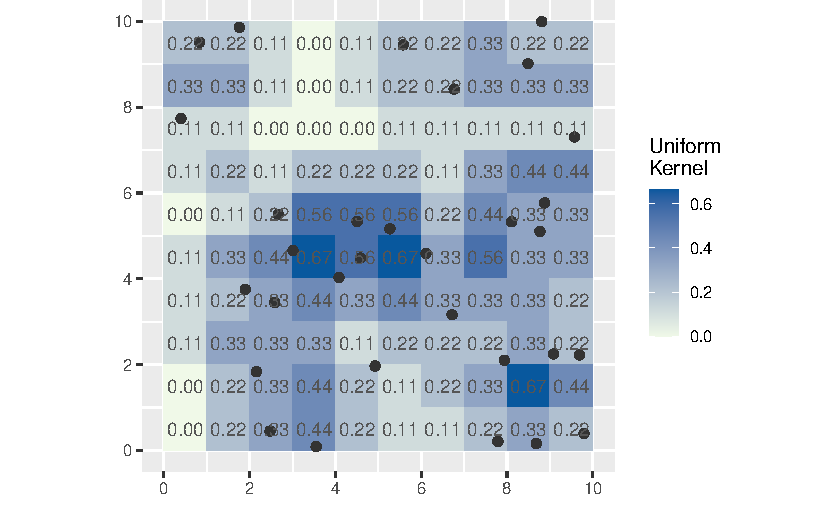
\includegraphics[keepaspectratio]{14_ppa_1st_files/figure-pdf/fig-kernel01-1.pdf}}

}

\caption{\label{fig-kernel01}Example of kernel density estimation using
a 3 × 3 uniform kernel. A density estimate is computed for each cell by
counting the points within the kernel window and dividing by the kernel
area. For example, the cell centered at (x=1.5, y=7.5) contains one
point within its 3 × 3 unit neighborhood and therefore has a local
density estimate of 1/9=0.11.}

\end{figure}%

Not all kernel functions assign equal weight to points within the kernel
window. More commonly, points closer to the center of the kernel receive
greater weight than points farther away. Many kernel functions follow a
\emph{Gaussian} or \emph{quartic} distribution, causing the influence of
a point to decrease with distance from the kernel center. These
weighting schemes tend to produce smoother estimates of spatial
intensity.

\begin{figure}[H]

\centering{

\pandocbounded{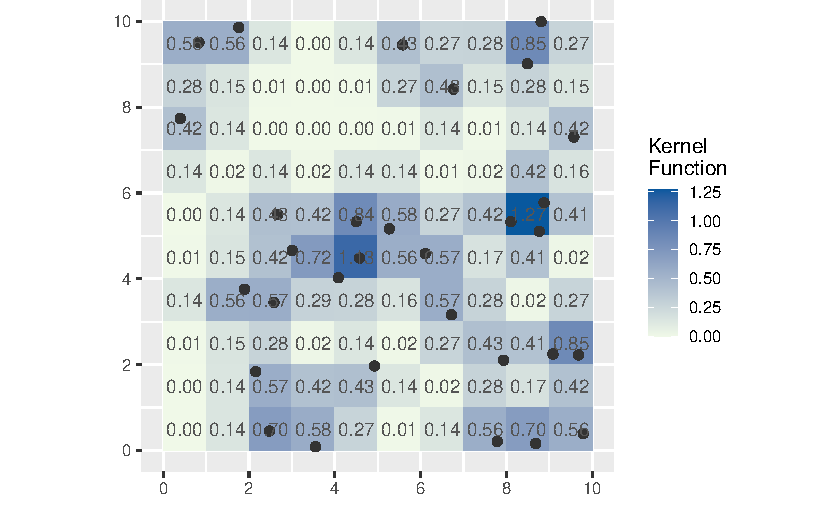
\includegraphics[keepaspectratio]{14_ppa_1st_files/figure-pdf/fig-kernel02-1.pdf}}

}

\caption{\label{fig-kernel02}Example of kernel density estimation using
a 3 × 3 quartic kernel. Each point within the kernel window contributes
to the density estimate according to its distance from the kernel
center, with nearby points receiving greater weight. The resulting
intensity surface is smoother than that produced by the uniform kernel
shown in Figure~\ref{fig-kernel01}.}

\end{figure}%

While kernel density estimation produces a smooth map of estimated point
intensity, it remains primarily a descriptive tool. A common exploratory
step is to compare the resulting intensity surface to an underlying
covariate such as elevation, land cover, or population density. This can
help identify potential spatial relationships, for instance, whether
areas of high point intensity tend to correspond to areas with high
covariate values. Such comparisons can provide useful clues about the
processes shaping the point pattern, but they do not directly model the
relationship between intensity and the covariate. To do that, we need
methods that explicitly estimate intensity as a function of one or more
covariates.

\subsection{Non-parametric Intensity Modeling with
Covariates}\label{non-parametric-intensity-modeling-with-covariates}

In an earlier section, we learned that we could use a covariate, such as
elevation, to define the sub-regions (quadrats) within which densities
were computed.

Here, instead of dividing the study region into discrete sub-regions, we
estimate an \textbf{intensity function}, denoted \(\rho(z)\), that
describes how point intensity varies as a function of a covariate \(z\)
(e.g., elevation). This function is then used to model the spatial
intensity \(\widehat{\lambda}(x)\) at each location \(x\) in the study
area.

In this framework, \(\rho(z)\) describes the relationship between
intensity and the covariate, whereas \(\widehat{\lambda}(x)\) represents
the resulting intensity surface across the study region after applying
that relationship to the spatial distribution of the covariate.

Several approaches can be used to estimate \(\rho(z)\) including the
\emph{ratio}, \emph{re-weight} and \emph{transform} methods. We will not
examine the differences among these methods here, but it is worth noting
that there is more than one way to estimate the relationship between
intensity and a covariate.

In the following example, elevation is used as the covariate and
\(\rho(z)\) is estimated using the \emph{ratio} method. This method
compares the observed density of points at different covariate values to
the density of the covariate itself, producing an estimate of relative
intensity. The resulting \(\rho(z)\) function is shown in the center
panel, while the right panel maps the modeled spatial intensity
\(\widehat{\lambda}(x)\) derived from the elevation surface.

\begin{figure}[H]

\centering{

\pandocbounded{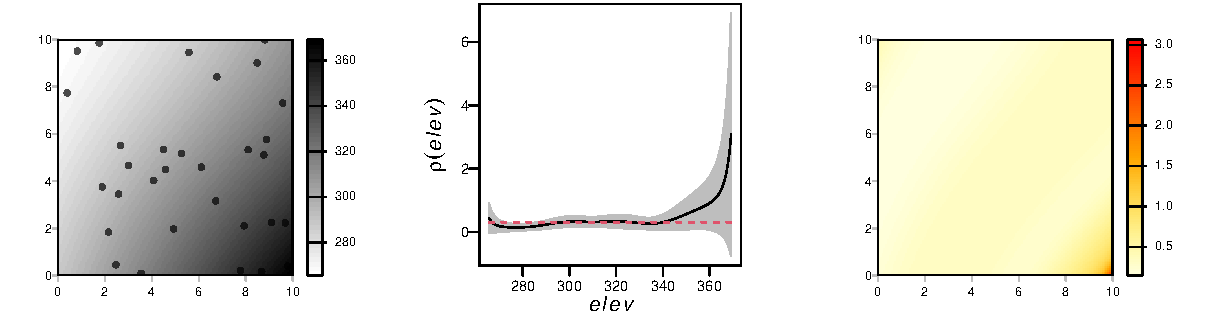
\includegraphics[keepaspectratio]{14_ppa_1st_files/figure-pdf/fig-kernel03-1.pdf}}

}

\caption{\label{fig-kernel03}Non-parametric estimation of intensity as a
function of elevation using the ratio method. The left panel shows the
observed point pattern superimposed on the elevation raster. The center
panel shows the estimated intensity function, \(\rho(z)\) as a function
of elevation; the shaded envelope represents the 95\% confidence
interval. The right panel maps the modeled spatial intensity,
\(\widehat{\lambda}(x)\), obtained by applying the estimated \(\rho(z)\)
relationship to the elevation raster.}

\end{figure}%

One way to assess how well the covariate explains the observed point
pattern is to compare the modeled intensity surface to the observed
intensity surface derived from kernel density estimation. The following
scatter plot compares the modeled intensity values to the observed
kernel density estimates at corresponding locations.

\begin{figure}[H]

\centering{

\pandocbounded{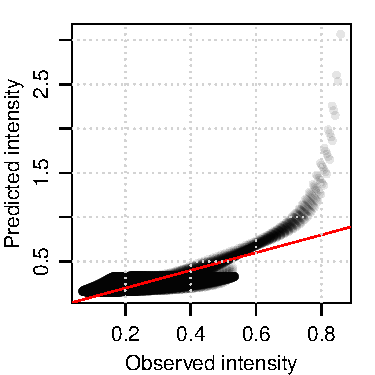
\includegraphics[keepaspectratio]{14_ppa_1st_files/figure-pdf/fig-kernel04-1.pdf}}

}

\caption{\label{fig-kernel04}Comparison of modeled intensity and
observed kernel density estimates. Each point represents a location in
the study area, with the x-axis showing the observed kernel density and
the y-axis showing the intensity predicted from elevation. The red
diagonal line represents perfect agreement between observed and
predicted intensity.}

\end{figure}%

A red one-to-one diagonal line is added to the plot. The scatter plot
compares the modeled intensity (based on elevation) to the observed
kernel density estimates. While the overall relationship is positive,
the points deviate from the one-to-one line, indicating that the
elevation-based model does not perfectly reproduce the observed
intensity surface.

Some of this discrepancy may reflect increased uncertainty at higher
elevation values, where fewer observations are available to estimate the
relationship between intensity and elevation. This uncertainty is
evident in the \(\rho(z)\) \emph{vs.~elevation} plot
(Figure~\ref{fig-kernel03}) where the 95\% confidence envelope widens at
higher elevations. Such widening is common in spatial modeling when
covariate values are unevenly represented across the study area.

Modeling intensity as a function of a covariate allows us to explore
first-order effects more rigorously. It helps determine whether external
factors, such as elevation or population density, can explain the
spatial distribution of points.

While this approach still relies on kernel-based methods, it differs
conceptually from the kernel density estimation introduced in the
previous section. Standard kernel density estimation uses only the
observed point locations to estimate intensity and can then be compared
to a covariate map to identify potential associations. Here, however,
the covariate is \emph{incorporated} directly into the estimation
procedure. Instead of asking whether a density surface resembles a
covariate, we explicitly estimate how intensity changes as a function of
that covariate.

This approach yields a non-parametric estimate of the relationship
between intensity and a covariate, providing insight into first-order
effects. The function \(\rho(z)\) captures this relationship without
assuming a specific parametric form. In the next section, we explore a
complementary approach, \textbf{Poisson point process modeling}, which
specifies intensity as a parametric log-linear function of one or more
covariates.

\subsection{Parametric Intensity Modeling with
Covariates}\label{parametric-intensity-modeling-with-covariates}

Up to this point, we have focused on non-parametric techniques for
describing how point intensity varies across space and with underlying
covariates. While these methods can reveal important first-order
patterns, they do not provide an explicit statistical model relating
intensity to a covariate. In many applications, it is useful to specify
this relationship directly using a formal statistical framework.

\begin{quote}
\textbf{Note:} A useful way to think about the difference between
parametric and non-parametric approaches is that \textbf{parametric
models summarize a relationship with a few numbers}, whereas
\textbf{non-parametric models summarize a relationship with a fitted
curve whose shape is determined largely by the data}. In the previous
section, the \(\rho(z)\) function was estimated without assuming a
specific mathematical form. In this section, we assume a specific
log-linear form whose shape is determined by a small set of parameters.
\end{quote}

One widely used approach is the \textbf{Poisson point process model
(PPM)} which expresses point intensity as a function of one or more
covariates. A simple PPM takes the form:

\begin{equation}
\lambda(i) = e^{\alpha + \beta Z(i)}
\label{eq:density-covariate}
\end{equation}

This equation defines how the expected point intensity varies as a
function of the covariate \(Z(i)\). The term \(\lambda(i)\) represents
the modeled intensity at location \(i\), while \(e^{\alpha}\) is the
baseline intensity when the covariate is \emph{zero}. The term
\(e^{\beta}\) represents the multiplicative change in intensity
associated with a one-unit increase in the covariate \(Z(i)\). The
parameters \(\alpha\) and \(\beta\) are estimated from the data using
maximum likelihood, a procedure that identifies the parameter values
that best explain the observed point pattern given the covariate
surface. Note that the units of intensity are determined by the
coordinate reference system (for example, stores per square kilometer),
and the interpretation of \(\beta\) depends on the scale and units of
the covariate.

The equation is a form of a \textbf{log-linear} model commonly used in
spatial statistics to model intensity. While it resembles logistic
regression in structure, the quantity being modeled is different. In a
Poisson point process model, the response variable is
\textbf{intensity}, whereas logistic regression models
\textbf{probability}. Taking the natural logarithm of both sides yields
the more familiar linear form:

\[
\log{\lambda}(i) = \alpha + \beta Z(i)
\] where \(\alpha + \beta Z(i)\) is the \textbf{linear predictor}.

\begin{quote}
Note: The log-linear form of a Poisson point process model resembles
that of logistic regression, a model many students may have encountered
in an introductory statistics course. However, the two approaches serve
different purposes. Logistic regression models the probability of
occurrence, while a Poisson point process model models the intensity of
occurrence. Although mathematical connections exist between these
frameworks, they should not be interpreted as equivalent models. One
such connection is given by the transformation
\(\lambda = P / (1 - P)\), which leads to: \[
P(i) = \frac{e^{\alpha + \beta Z(i)}}{1 + e^{\alpha + \beta Z(i)}}
\]
\end{quote}

This relationship is useful when interpreting intensity in terms of
probability, particularly in presence/absence modeling.

The Poisson point process model assumes that events occur independently
and that intensity varies smoothly as a function of the covariate. It
does not account for interactions among points and is therefore designed
to model \emph{first-order effects} rather than the \textbf{second-order
interactions} examined in the next chapter.

The advantage of this framework is that it provides both parameter
estimates and formal statistical tests for assessing whether a covariate
contributes to explaining the observed point pattern.

To illustrate, consider the distribution of Starbucks cafés in
Massachusetts. The point pattern is clearly non-uniform, suggesting that
café locations may be influenced by underlying socioeconomic factors.
One plausible covariate is population density, since areas with larger
populations may support a greater number of retail establishments. The
following figure compares Starbucks locations to the population density
distribution.

\begin{figure}[H]

\centering{

\pandocbounded{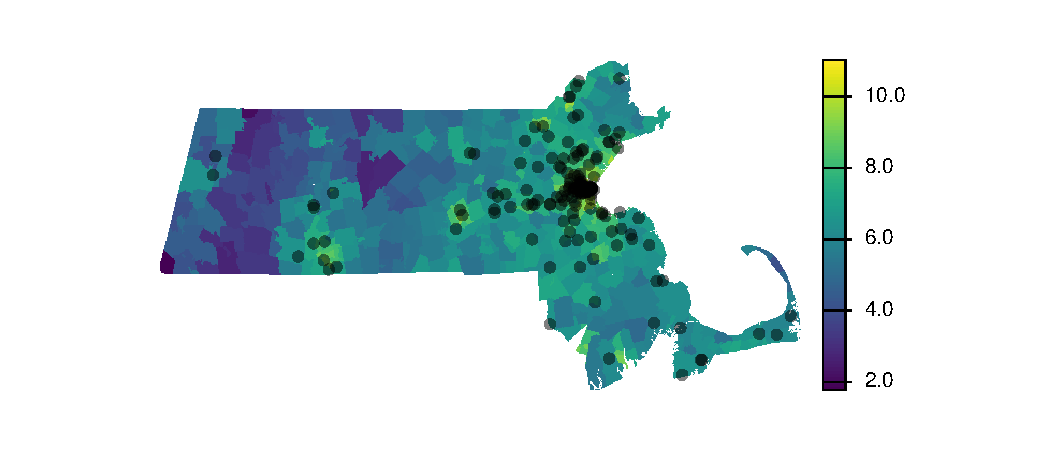
\includegraphics[keepaspectratio]{14_ppa_1st_files/figure-pdf/fig-starbucks-1.pdf}}

}

\caption{\label{fig-starbucks}Location of Starbucks cafés in
Massachusetts overlaid on population density. The apparent concentration
of stores in densely populated areas suggests that population density
may be an important predictor of point intensity. Note that the
population density classes are displayed on a logarithmic scale to
better differentiate values.}

\end{figure}%

We can fit a Poisson point process model to these data where the modeled
intensity takes the form:

\begin{equation}
Starbucks\ intensity(i) = e^{\alpha + \beta\ population(i)}
\label{eq:walmart-model}
\end{equation}

The parameters \(\alpha\) and \(\beta\) are typically estimated using a
procedure called \emph{maximum likelihood}. Its implementation is not
covered here but is widelydiscussed in introductory statistics
textbooks. The index \((i)\) reminds us that both the modeled intensity
and the population density can vary as a function of location.

In our example, the estimated value of \(\alpha\) is -5.151. This
indicates that when population density is \emph{zero}, the baseline
intensity of the point process is e\textsuperscript{-5.151} = 0.00579
cafes per square kilometer (the units are determined by the coordinate
reference system), a value close to zero as one might expect.

The estimated value of \(\beta\) is 0.00017. This indicates that for
every one-unit increase in the population density raster, the intensity
of the point process is multiplied by e\textsuperscript{0.00017} =
1.00017.

Thus, higher population density is associated with a higher expected
intensity of Starbucks locations.

The following figure shows the fitted intensity function as a function
of population density, along with a 95\% confidence envelope. This plot
helps visualize the estimated relationship between population density
and store intensity while highlighting uncertainty in the fitted model.

\begin{figure}[H]

\centering{

\pandocbounded{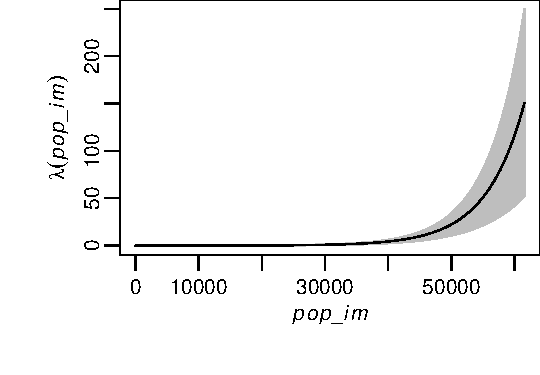
\includegraphics[keepaspectratio]{14_ppa_1st_files/figure-pdf/fig-pppm01-1.pdf}}

}

\caption{\label{fig-pppm01}Poisson point process model fitted to the
relationship between Starbucks café locations and population density.
The fitted curve represents the estimated intensity of Starbucks
locations as a function of population density, while the shaded envelope
shows the 95\% confidence interval. The model assumes a log-linear
relationship between intensity and the covariate. Intensity is reported
as the expected number of stores per square kilometer.}

\end{figure}%

Fitting a Poisson point process model provides an estimate of how
intensity varies with a covariate. However, the presence of a fitted
relationship does not necessarily imply that the covariate meaningfully
improves our understanding of the observed point pattern. In the next
section, we compare the covariate-based model to a simpler null model
(e.g., a homogeneous intensity model) using formal statistical tests.
This allows us to assess whether the covariate explains a significant
portion of the observed variation in point intensity.

\section{Hypothesis Testing for Covariate Effects}\label{PPM}

A Poisson point process model can always be fitted to an observed point
pattern, but the presence of a fitted relationship does not necessarily
imply that the covariate meaningfully explains the observed distribution
of points. To assess whether a covariate improves our understanding of
the point pattern, we compare the fitted model to a simpler alternative.

In this framework, a model that assumes homogeneous intensity across
space serves as the \textbf{null hypothesis}, while a model that allows
intensity to vary as a function of a covariate serves as the
\textbf{alternative hypothesis}.

For example, we may wish to determine whether the spatial distribution
of Walmart stores is better explained by population density than by a
model that assumes no spatial preference. In other words, we want to
assess whether variation in store intensity can reasonably be attributed
to population density rather than to random variation alone.

The following figure shows Walmart store locations relative to
population density in Massachusetts.

\begin{figure}[H]

\centering{

\pandocbounded{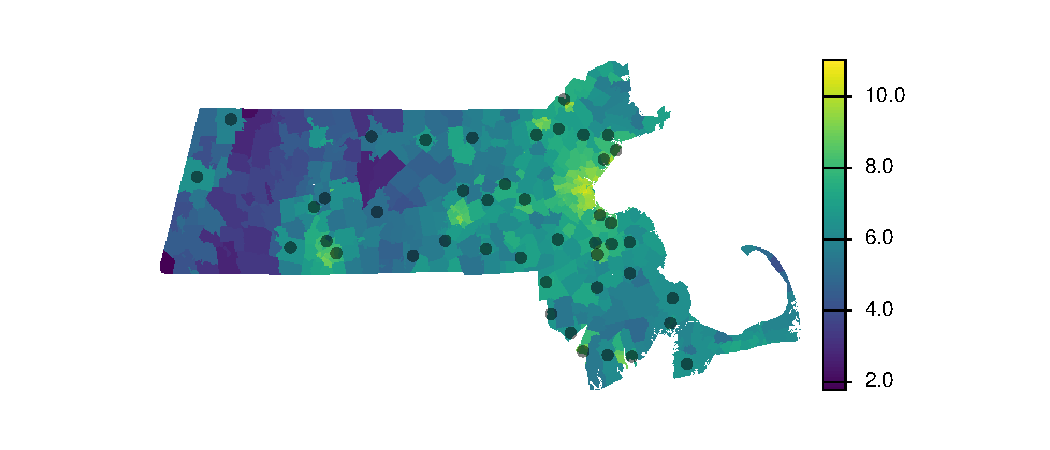
\includegraphics[keepaspectratio]{14_ppa_1st_files/figure-pdf/fig-walmarts-1.pdf}}

}

\caption{\label{fig-walmarts}Walmart store locations and population
density in Massachusetts. This figure motivates the hypothesis that
store intensity may vary as a function of population density rather than
remaining constant across the study area. Population density values are
displayed on a logarithmic scale.}

\end{figure}%

To determine whether population density provides a meaningful
explanation for the observed Walmart distribution, we fit both the null
and alternative models and compare their fit using a \textbf{likelihood
ratio test}. This test evaluates whether the additional complexity of
the covariate-based model is justified by a significantly better fit to
the observed point pattern.

A Poisson point process model fitted to the Walmart point pattern using
the \texttt{ppm} function in the \texttt{spatsat} package (Baddeley et
al. 2016) produces the following output for the null model:

\begin{verbatim}
Stationary Poisson process
Fitted to point pattern dataset 'P'
Intensity: 0.0021276
             Estimate      S.E.   CI95.lo   CI95.hi Ztest     Zval
log(lambda) -6.152761 0.1507557 -6.448236 -5.857285   *** -40.8128
\end{verbatim}

Whereas the null model assumes a constant intensity across the study
area, the alternative model allows intensity to vary with population
density. Fitting this model produces the following output:

\begin{verbatim}
Nonstationary Poisson process
Fitted to point pattern dataset 'P'

Log intensity:  ~pop

Fitted trend coefficients:
  (Intercept)           pop 
-6.2551180493  0.0001043115 

                 Estimate         S.E.       CI95.lo       CI95.hi Ztest
(Intercept) -6.2551180493 1.611991e-01 -6.571062e+00 -5.9391736579   ***
pop          0.0001043115 3.851572e-05  2.882207e-05  0.0001798009    **
                  Zval
(Intercept) -38.803683
pop           2.708284
Problem:
 Values of the covariate 'pop' were NA or undefined at 0.7% (4 out of 572) of 
the quadrature points
\end{verbatim}

Using the estimated coefficients from the fitted models, we can express
the intensity functions explicitly.

The null model, which assumes homogeneous intensity across the study
area, takes the form:

\[
\lambda(i) = e^{-6.2}
\]

The alternative model, which allows intensity to vary as a function of
population density, takes the form:

\[
\lambda(i) = e^{-6.3 + 1.04\times10^{-4}population}
\]

To better understand how these models differ, we can visualize the
estimated intensity (\(\widehat{\lambda}\)) as a function of population
density for both the null and alternative models.

\begin{figure}[H]

\centering{

\pandocbounded{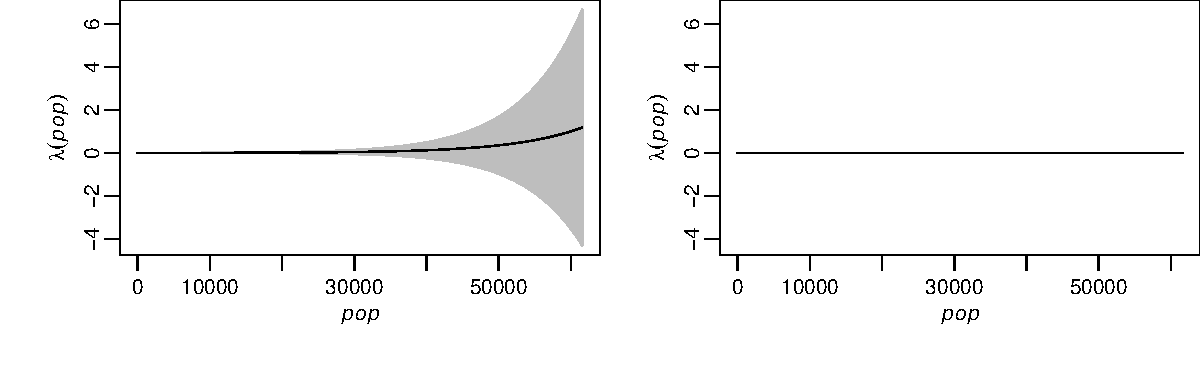
\includegraphics[keepaspectratio]{14_ppa_1st_files/figure-pdf/fig-Ho_vs_H-1.pdf}}

}

\caption{\label{fig-Ho_vs_H}Estimated intensity functions from the
Poisson point process models. The left panel shows the alternative
model, in which intensity varies as a function of population density,
while the right panel shows the null model, which assumes a constant
intensity across the study area. Shaded envelopes represent 95\%
confidence intervals.}

\end{figure}%

The fitted intensity functions clearly differ, but this does not
necessarily imply that the population-density model provides a
significantly better explanation of the observed point pattern than the
null model. The relatively wide confidence intervals associated with the
covariate-based model, especially at higher population densities,
suggest uncertainty in the estimated relationship. This highlights the
need for formal statistical testing before concluding that population
density contributes meaningfully to the observed variation in store
intensity.

To formally assess whether the covariate-based model provides a
significantly better fit than the null model, we use a likelihood ratio
test. This test compares the log-likelihoods of the two models and
evaluates whether the improvement in fit achieved by the more complex
model is greater than would be expected by chance alone.

\begin{verbatim}
Analysis of Deviance Table

Model 1: ~1      Poisson
Model 2: ~pop    Poisson
  Npar Df Deviance Pr(>Chi)  
1    5                       
2    6  1   4.2531  0.03918 *
---
Signif. codes:  0 '***' 0.001 '**' 0.01 '*' 0.05 '.' 0.1 ' ' 1
\end{verbatim}

The value reported under \texttt{PR(\textgreater{}Chi)} is the p-value.
It represents the probability of observing an improvement in fit at
least as large as the one obtained here if the null model were true. In
our example, the resulting p-value is 0.039. This indicates that, under
the assumption of homogeneous intensity, there is approximately a 3.9\%
chance of observing a difference between the two models this large or
larger simply due to random variation. Because this probability is
small, the results provide evidence that population density improves our
ability to explain the spatial distribution of Walmart stores.

In summary, the likelihood ratio test suggests that population density
is a meaningful covariate for explaining variation in Walmart store
intensity. While uncertainty remains in the estimated relationship, the
covariate-based model provides a significantly better fit than the
homogeneous-intensity model.

\section{Summary}\label{summary-12}

This chapter introduced methods for analyzing \textbf{first-order
effects} in spatial point patterns. Rather than focusing on interactions
among points, first-order analyses seek to understand how point
intensity varies across space and how that variation may be related to
underlying environmental or socioeconomic factors.

\begin{itemize}
\tightlist
\item
  \textbf{Intensity} refers to the underlying rate at which events occur
  across space, whereas density refers to the observed number of points
  per unit area.
\item
  A \textbf{homogeneous} point process assumes constant intensity across
  the study area, while an \textbf{inhomogeneous} process allows
  intensity to vary spatially.
\item
  \textbf{Global density} provides a single estimate of intensity for an
  entire study region and serves as a useful baseline summary measure.
\item
  \textbf{Local density} methods allow intensity to be estimated at
  different locations, helping identify spatial variation that may
  indicate first-order effects.
\item
  \textbf{Quadrat density} estimates local intensity by partitioning the
  study area into subregions, but results can be sensitive to quadrat
  size and placement, an example of the modifiable areal unit problem
  (MAUP).
\item
  \textbf{Kernel density estimation (KDE)} replaces fixed quadrats with
  a moving window, producing a smoother representation of spatial
  intensity.
\item
  Density and intensity surfaces can be compared to covariates such as
  elevation or population density to explore potential explanations for
  spatial variation in point intensity.
\item
  \textbf{Non-parametric intensity modeling} estimates the relationship
  between intensity and a covariate without assuming a specific
  functional form.
\item
  Poisson point process models (PPMs) provide a parametric framework for
  expressing intensity as a function of one or more covariates.
\item
  PPMs focus on \textbf{first-order effects}, assuming that events occur
  independently and that intensity varies as a function of external
  factors rather than interactions among points.
\item
  \textbf{Likelihood ratio tests} can be used to compare a
  covariate-based intensity model to a simpler homogeneous-intensity
  model, allowing us to assess whether a covariate significantly
  improves our understanding of the observed point pattern.
\item
  Throughout this chapter, the emphasis has been on explaining where
  point intensity is high or low and why it varies across space. In the
  next chapter, we turn our attention to \textbf{second-order effects},
  asking whether points exhibit clustering, dispersion, or interaction
  beyond what would be expected from the underlying intensity surface
  alone.
\end{itemize}

\chapter{Second-Order Point Pattern
Analysis}\label{second-order-point-pattern-analysis}

\section{Introduction}\label{introduction-14}

An alternative to the \emph{density-based methods} explored in Chapter
14 are \textbf{distance-based methods} for analyzing spatial point
patterns. Whereas Chapter 14 focused on \textbf{first-order effects} by
modeling how point intensity varies across space, distance-based methods
focus on \textbf{second-order effects} by examining how points are
distributed \textbf{relative to one another}. This shift enables us to
explore whether events exhibit spatial interaction, such as
\textbf{clustering} or \textbf{dispersion}, across various spatial
scales.

Distance-based methods are particularly useful when the goal is to
assess whether the observed pattern deviates from what would be expected
under complete spatial randomness (CSR), a benchmark model in spatial
statistics. Rather than estimating intensity across space, these methods
examine the spatial arrangement of points directly through inter-point
distances. Importantly, because first-order effects can create the
appearance of clustering, the methods introduced in this chapter are
often applied only after considering whether spatial variation in
intensity may be present.

In this chapter, we begin with the \textbf{Average Nearest Neighbor
(ANN)} statistic, a simple distance-based measure that provides an
intuitive introduction to second-order point pattern analysis. We then
explore the \textbf{hypothesis-testing} framework used to assess
second-order effects, including Monte Carlo simulation and methods for
controlling underlying first-order variation. Finally, we introduce
additional distance-based statistics, including Ripley's K and L
functions and the Pair Correlation Function (PCF), which provide
alternative ways of summarizing spatial interaction across multiple
scales.

\section{Average Nearest Neighbor}\label{average-nearest-neighbor}

\textbf{Average Nearest Neighbor (ANN)} analysis measures the average
distance from each point in a study area to its nearest neighboring
point. Because it focuses on distances between points, ANN provides a
simple and intuitive way to quantify spatial interaction. The statistic
summarizes the spatial arrangement of points and can help distinguish
between clustered, random, or regularly spaced patterns.

In the example below, the average nearest neighbor distance for all
points is 13,295 meters.

\begin{figure}[H]

\centering{

\pandocbounded{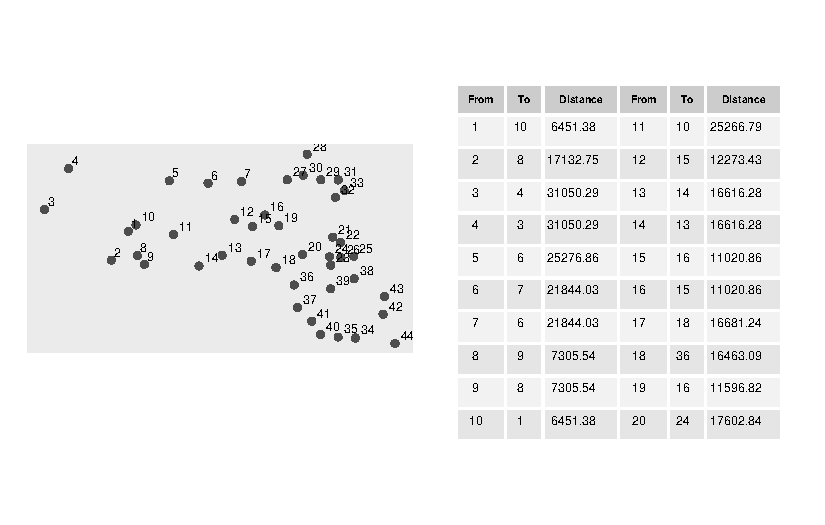
\includegraphics[keepaspectratio]{15_ppa_2nd_files/figure-pdf/fig-ppp_dist-1.pdf}}

}

\caption{\label{fig-ppp_dist}The table shows a subset of
nearest-neighbor distances used to compute the Average Nearest Neighbor
(ANN) statistic. For example, the point closest to point 3 is point 4,
which is 16,616 meters away.}

\end{figure}%

While ANN is traditionally defined using only the nearest neighbor, the
same concept can be extended to second, third, and higher-order
neighbors. Doing so reveals how inter-point distances change as
progressively farther neighbors are considered. This produces a curve
that reflects how the spatial structure of the pattern changes with
neighbor order.

\begin{figure}[H]

\centering{

\pandocbounded{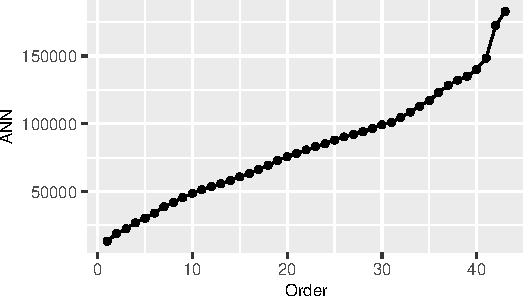
\includegraphics[keepaspectratio]{15_ppa_2nd_files/figure-pdf/fig-ann_plot-1.pdf}}

}

\caption{\label{fig-ann_plot}ANN values for different neighbor order
numbers. For example, the ANN for the first closest neighbor for all
points is 13,295 meters; the ANN for the 2nd closest neighbor for all
points is 18850 meters, and the ANN for the 43rd closest neighbor (the
furthest neighbor) for all points is 182,818 meters.}

\end{figure}%

The shape of the ANN curve provides insight into the spatial structure
of the pattern. A steep initial slope followed by a gradual increase may
indicate tight clustering, whereas a more linear increase suggests a
more regularly spaced arrangement.

To illustrate how ANN curves vary with different spatial arrangements,
consider three point patterns of 20 points each:

\begin{itemize}
\tightlist
\item
  A single cluster
\item
  A dual cluster
\item
  A random scatter
\end{itemize}

\begin{figure}[H]

\centering{

\pandocbounded{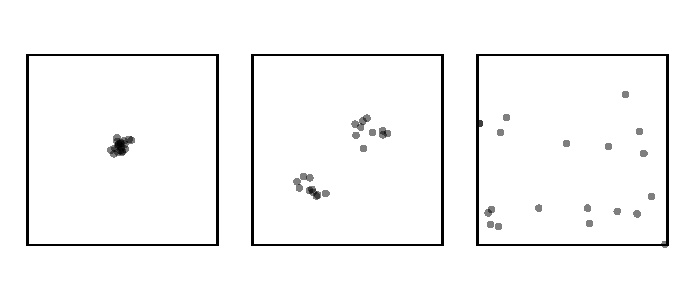
\includegraphics[keepaspectratio]{15_ppa_2nd_files/figure-pdf/fig-diff_patterns-1.pdf}}

}

\caption{\label{fig-diff_patterns}Three hypothetical point patterns used
to illustrate how ANN responds to different spatial structures: a single
cluster, a dual cluster, and a randomly scattered pattern.}

\end{figure}%

The following figure illustrates how the ANN curve varies across three
spatial arrangements, highlighting the sensitivity of ANN to clustering
structure.

\begin{figure}[H]

\centering{

\pandocbounded{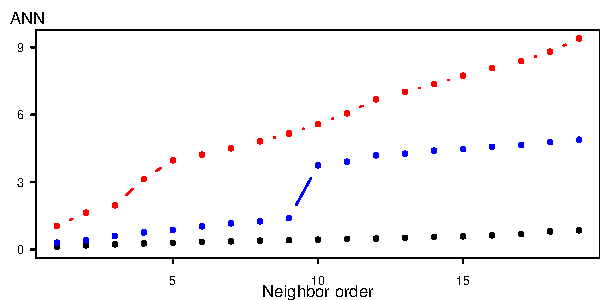
\includegraphics[keepaspectratio]{15_ppa_2nd_files/figure-pdf/fig-diff_ann_plots-1.pdf}}

}

\caption{\label{fig-diff_ann_plots}Three different ANN vs.~neighbor
order plots. The black ANN line is for the first point pattern (single
cluster); the blue line is for the second point pattern (double cluster)
and the red line is for the third point pattern.}

\end{figure}%

\begin{itemize}
\tightlist
\item
  The black line (single cluster) shows short distances across all
  neighbor orders, indicating tight clustering.
\item
  The blue line (dual cluster) shows intermediate distances, reflecting
  the presence of two separate clusters.
\item
  The red line (random scatter) shows longer distances overall,
  consistent with a more dispersed arrangement.
\end{itemize}

The perceived spatial structure of a point pattern is highly sensitive
to the definition of the study area. In the example below, the same
clustered pattern is shown within two different bounding boxes:

\begin{figure}[H]

\centering{

\pandocbounded{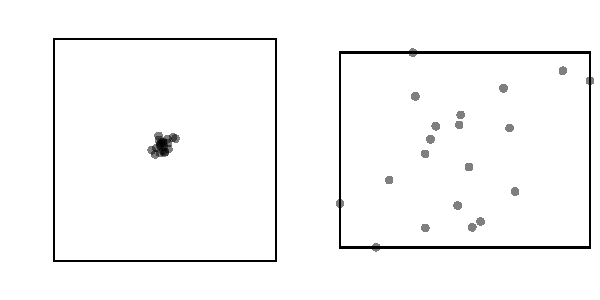
\includegraphics[keepaspectratio]{15_ppa_2nd_files/figure-pdf/fig-diff_ppp02-1.pdf}}

}

\caption{\label{fig-diff_ppp02}The same point pattern shown within two
different study extents. Differences in perceived clustering illustrate
the sensitivity of point pattern analysis to study area definition and
the influence of the modifiable areal unit problem (MAUP).}

\end{figure}%

When the study area is tightly fitted around the cluster, the pattern
appears more dispersed than when the same points are viewed within a
larger study extent. This example highlights the importance of study
area definition and serves as another illustration of the modifiable
areal unit problem (MAUP).

Like most distance-based point pattern statistics, ANN assumes that the
underlying point process is stationary, meaning that the intensity of
the process does not vary across space. If the process is non-stationary
(or inhomogeneous), apparent clustering may simply reflect underlying
environmental or socioeconomic gradients rather than true interaction
among points.

This distinction is important because the goal of second-order analysis
is to detect interactions among points after accounting for any
large-scale variation in intensity. In the next section, we introduce
hypothesis-testing approaches that allow us to assess whether an
observed pattern is consistent with complete spatial randomness and how
those tests can be adapted when first-order effects are present.

\section{Hypothesis Testing for Second-Order
Effects}\label{hypothesis-testing-for-second-order-effects}

\subsection{Analytical Tests}\label{analytical-tests}

A fundamental question in second-order point pattern analysis is whether
the observed arrangement of points differs from what would be expected
under \textbf{Complete Spatial Randomness (CSR)}. CSR serves as a
benchmark model in which points are assumed to occur independently and
with constant intensity across the study area. If the observed pattern
departs from CSR, then there may be evidence of clustering, dispersion,
or some underlying spatial process.

Several approaches can be used to test for departures from CSR. We begin
with an analytical test based on the \textbf{Average Nearest Neighbor
(ANN)} statistic and then proceed to a more flexible Monte Carlo
framework.

The analytical approach compares the observed mean nearest neighbor
distance to the distance expected under a CSR process. The null
hypothesis assumes that the observed point pattern is a realization of a
spatially uniform and independent process.

Under CSR, the expected mean nearest neighbor distance is:

\[
ANN_{expected}=\dfrac{1}{2\sqrt{n/A}}
\]

where:

\begin{itemize}
\tightlist
\item
  \(n\) is the number of points;
\item
  \(A\) is the area of the study region.
\end{itemize}

The analytical test compares the observed ANN value to the ANN value
expected under CSR. If the observed value is substantially smaller than
expected, the points may be clustered. If it is substantially larger,
the points may be dispersed.

The test statistic is the ratio:

\[
R = \frac{ANN_{observed}}{ANN_{expected}}
\]

Interpretation:

\begin{itemize}
\tightlist
\item
  \(R < 1\): suggests clustering
\item
  \(R > 1\): suggests dispersion
\item
  \(R \approx 1\) suggests a pattern consistent with Complete Spatial
  Randomness (CSR)
\end{itemize}

To assess statistical significance, a z-score is computed:

\[
z = \frac{ANN_observed - ANN_expected}{SE}
\] where the standard error (SE) of the expected distance under CSR is:

\[
SE = \frac{0.26136}{\sqrt{n\lambda}}
\] This z-score is then compared to a standard normal distribution to
determine whether the observed pattern deviates significantly from CSR.

While analytically elegant, the ANN hypothesis test has several
limitations that constrain its interpretive power:

\begin{itemize}
\item
  \textbf{Sensitivity to Study Area Definition:} The expected distance
  depends on the area \(A\), which must be defined explicitly.
\item
  \textbf{Shape Effects:} The formula assumes a regularly shaped study
  region. Irregular boundaries distort the expected distance and
  introduce edge effects, where points near the boundary have
  artificially inflated nearest-neighbor distances.
\item
  \textbf{Stationarity Assumption:} The test assumes a stationary
  process, meaning that intensity is constant across space. If the
  underlying process is inhomogeneous, with point density varying due to
  environmental or socioeconomic factors, apparent clustering may
  reflect first-order effects rather than true inter-point interaction.
\end{itemize}

\subsection{Monte Carlo Tests}\label{monte-carlo-tests}

While the analytical approach to ANN hypothesis testing offers a
convenient benchmark for assessing spatial randomness, its reliance on
idealized assumptions, such as a regularly shaped study area, can limit
its applicability in real-world settings. When these assumptions are
violated, the analytical test may yield misleading results. To address
these limitations, spatial analysts often turn to simulation-based
methods such as \textbf{Monte Carlo techniques}, which provide a more
flexible and empirically grounded framework for hypothesis testing.

The key idea behind Monte Carlo testing is simple: if we can simulate
many realizations of a hypothesized process, we can compare our observed
pattern to the patterns generated under that hypothesis. This allows us
to assess whether the observed pattern is unusual or whether it could
plausibly have arisen from the hypothesized process.

The Monte Carlo technique involves three steps:

\begin{itemize}
\item
  First, we specify a \textbf{null hypothesis}, \(H_0\). For example, we
  might hypothesize that the distribution of Walmart stores is
  consistent with \textbf{Complete Spatial Randomness (CSR)}.
\item
  Next, we generate many realizations of the hypothesized process and
  compute a statistic (e.g., ANN) for each realization.
\item
  Finally, we compare the observed statistic to the distribution of
  simulated statistics and assess whether the observed pattern is
  consistent with the hypothesized process.
\end{itemize}

Using the Walmart store distribution as an example, we randomly
reposition the Walmart locations 1,000 times (or as many times as
computationally practical) according to a CSR process, our hypothesized
process \(H_0\), while ensuring that all simulated locations remain
within the study area (the state of Massachusetts).

\begin{figure}[H]

\centering{


\includegraphics[width=3.125in,height=\textheight,keepaspectratio]{img/Sample_rnd_pts.png}

}

\caption{\label{fig-sim_points_example}Three realizations of a Complete
Spatial Randomness (CSR) process. Each simulation represents one
possible point pattern that could arise if Walmart locations were
distributed independently and with constant intensity throughout the
study area.*}

\end{figure}%

For each realization of our hypothesized process, we compute an ANN
value. Because each simulated pattern is different, the resulting ANN
values also differ. Collectively, these values form an \textbf{empirical
sampling distribution} under the null hypothesis of Complete Spatial
Randomness (CSR). In other words, the distribution shows the range of
ANN values we would expect to observe if CSR were the process generating
the point pattern. We can summarize this distribution with a histogram
and compare our observed ANN value of 13,294 m to the simulated values.

\begin{figure}[H]

\centering{


\includegraphics[width=4.16667in,height=\textheight,keepaspectratio]{img/ANN_hist.png}

}

\caption{\label{fig-walmart_MC_hist}Histogram of simulated ANN values
(from 1000 simulations). This is the sample distribution of the null
hypothesis, ANN\textsubscript{simulated} (under CSR). The red line shows
our observed (Walmart) ANN value. About 32\% of the simulated values are
greater (more extreme) than our observed ANN value.}

\end{figure}%

The histogram allows us to evaluate how unusual the observed ANN value
is relative to the values generated under CSR. If the observed value
falls near the center of the simulated distribution, the pattern may be
consistent with CSR. If it falls in one of the tails, then the observed
pattern may be inconsistent with the hypothesized process.

By using the same study region in each simulation, Monte Carlo methods
automatically account for edge effects and irregular study area shapes
(issues that are difficult to correct analytically).

\subsection{Estimating p-values}\label{estimating-p-values}

The histogram in Figure~\ref{fig-walmart_MC_hist} provides a visual
indication of how unusual the observed ANN value is relative to the
values generated under the null hypothesis. To quantify this comparison,
we compute a \textbf{Monte Carlo p-value}, which measures how often
simulated patterns produce a test statistic as extreme as the observed
one.

The \textbf{Monte Carlo p-value} represents the proportion of simulated
patterns that yield a test statistic more extreme than the observed one
under the null hypothesis. Specifically, we count how many simulated
values are \textbf{more extreme} than the observed statistic, either
greater or smaller, depending on the direction of the test.

For a \textbf{one-sided} test, the empirical p-value is calculated as:

\[
p = \dfrac{N_{extreme}+1}{N+1}
\]

where \emph{N\textsubscript{extreme}} is the number of simulated values
more extreme than our observed statistic, and \(N\) is the total number
of simulations. The \(+1\) is added to ensure that the p-value can never
be exactly 0.

In practice, a more general form of the equation is often used:

\[
p = \dfrac{min(N_{greater}+1 , N + 1 - N_{greater})}{N+1}
\]

where \(min(N_{greater}+1 , N + 1 - N_{greater})\) is the smallest of
the two values \(N_{greater}+1\) and \(N + 1 - N_{greater}\), and
\(N_{greater}\) is the number of simulated values greater than the
observed value. This formulation automatically determines which tail of
the simulated distribution is closer to the observed value. Because the
calculation can be cumbersome to perform manually, it is usually
implemented in software.

For example, suppose we ran 1,000 simulations in our ANN analysis and
found that 319 produced values more extreme than the observed ANN
statistic. The Monte Carlo p-value would then be

\[
p = \frac{319 + 1}{1000 + 1} = 0.32. 
\]

This can be interpreted as meaning that, if the null hypothesis of
\emph{Complete Spatial Randomness} (CSR) were true, there would be
approximately a \textbf{32\% chance of observing an ANN statistic at
least as extreme as the one obtained from the Walmart point pattern}.
Because this probability is relatively large, there is insufficient
evidence to reject the null hypothesis.

Importantly, this does not imply that Walmart stores were actually
located randomly across Massachusetts. Rather, it indicates that a CSR
process is one of many plausible processes that could have generated the
observed point pattern. In other words, the hypothesis test does not
identify the true process; it only assesses whether the observed pattern
is consistent with the hypothesized process.

If a two-sided test is desired, the p-value becomes:

\[
2 \times \dfrac{min(N_{greater}+1 , N + 1 - N_{greater})}{N+1}
\]

which is simply twice the smaller of the two tail probabilities.

Monte Carlo tests provide a robust alternative to analytical methods,
particularly when assumptions about study area shape or boundary effects
are difficult to satisfy. More importantly, they allow us to evaluate a
wide range of hypothesized processes, not just Complete Spatial
Randomness, making them one of the most versatile tools in spatial point
pattern analysis.

\subsection{Controlling for First-Order
Effects}\label{controlling-for-first-order-effects}

The assumption of CSR provides a useful baseline for spatial analysis,
but it is often unrealistic in real-world settings. Many spatial
processes exhibit both \emph{first-order effects} and \emph{second-order
effects}. When first-order effects are present, the underlying point
process is \emph{non-stationary} or \textbf{inhomogeneous}. In such
cases, hypothesis tests should account for this spatial heterogeneity.

\begin{figure}[H]

\centering{


\includegraphics[width=5.20833in,height=\textheight,keepaspectratio]{img/Pop_dens.png}

}

\caption{\label{fig-walmart_pop}Walmart store locations and population
density in Massachusetts. This figure motivates an alternative null
model in which point intensity varies as a function of population
density rather than remaining constant across the study area.}

\end{figure}%

For example, suppose we believe that the placement of Walmart stores is
influenced by population density. If so, then population density
represents a first-order effect that may explain part of the observed
spatial pattern. Under these circumstances, comparing the observed
pattern to a CSR process would be inappropriate because CSR assumes a
constant intensity across the study area.

Instead, we construct a more realistic null model in which point
intensity varies according to population density. We then use Monte
Carlo techniques to generate simulated point patterns from this
inhomogeneous process and compare the observed pattern to these
simulations.

\begin{figure}[H]

\centering{


\includegraphics[width=3.64583in,height=\textheight,keepaspectratio]{img/Non_hom_2.png}

}

\caption{\label{fig-walmart_pop_sim}Simulated realizations of an
inhomogeneous null model in which population density governs spatial
intensity. These patterns represent possible Walmart distributions if
population density were the sole factor influencing store intensity.}

\end{figure}%

Although we are no longer simulating a CSR process, the simulated
patterns are still random. The difference is that points are now placed
randomly \emph{according to} the underlying population density
distribution. Locations with higher population density therefore have a
greater chance of receiving simulated points than locations with lower
population density.

Using Monte Carlo techniques, we can generate thousands of such point
patterns and compare the observed ANN value to the ANN values computed
from the simulated patterns.

\begin{figure}[H]

\centering{


\includegraphics[width=3.125in,height=\textheight,keepaspectratio]{img/ANN_pop_dens.png}

}

\caption{\label{fig-ann_hetero_hist}Distribution of ANN values under a
null model where population density governs point intensity.}

\end{figure}%

In this example, the observed ANN value falls far to the right of the
simulated distribution, indicating that Walmart stores are more
dispersed than would be expected if population density were the sole
factor governing store placement. The proportion of simulated values
more extreme than the observed ANN value is approximately 0\% (i.e.~a
one-sided p-value \(\backsimeq\) 0.0), providing strong evidence against
this null model.

Another plausible hypothesis is that median household income influenced
the placement of Walmart stores.

\begin{figure}[H]

\centering{


\includegraphics[width=5.20833in,height=\textheight,keepaspectratio]{img/Median_income_map.png}

}

\caption{\label{fig-ann_income}Edge-corrected and uncorrected Pair
Correlation Function estimates for Walmart locations in Massachusetts.
Unlike the cumulative K and L functions, the PCF isolates spatial
interaction occurring at specific distances. The corrected PCF suggests
greater clustering than expected under CSR at distances exceeding
approximately 5 km.}

\end{figure}%

Running a Monte Carlo simulation using median household income as the
underlying intensity process yields an ANN distribution in which
approximately 16\% of the simulated values are more extreme than the
observed ANN value (i.e., a one-sided p-value of 0.16).

\begin{figure}[H]

\centering{


\includegraphics[width=3.64583in,height=\textheight,keepaspectratio]{img/Median_income_results.png}

}

\caption{\label{fig-ann_income_hist}Histogram of ANN values from
simulated point patterns generated under a median income-based intensity
model.}

\end{figure}%

We now have multiple competing null models. One assumes Complete Spatial
Randomness (CSR), while another assumes that point intensity varies with
median household income. Neither model can be rejected based on the
observed ANN statistic.

This serves as an important reminder that a hypothesis test cannot tell
us whether a \emph{particular} process is \emph{the} process responsible
for generating the observed point pattern. Instead, it tells us whether
the observed pattern is consistent with the hypothesized process.
Consequently, several different hypotheses may remain plausible
explanations for the same observed pattern.

It is also important to remember that ANN is fundamentally a
\emph{distance-based} measure of spatial interaction. Even though points
are simulated from an underlying intensity surface, our primary interest
remains the spacing of points \emph{relative to one another}. In other
words, we are not asking whether population density or income explains
the geographic locations of Walmart stores. That first-order question
was the focus of Chapter 14. Instead, we are asking whether evidence of
clustering or dispersion remains after accounting for a hypothesized
first-order effect. By controlling for covariates such as population
density or median household income, we can better isolate the
second-order interactions among points.

\subsection{Controlling for Second-Order
Effects}\label{controlling-for-second-order-effects}

While it is common practice to control for first-order effects when
testing for second-order spatial interaction, the reverse problem,
testing for first-order effects while accounting for second-order
interactions, is considerably more difficult.

The reason is that first-order effects can often be represented by an
intensity surface, \(\lambda(x)\), describing how the expected density
of points varies across space. Once this intensity surface has been
specified, it can be incorporated into Monte Carlo simulations and used
as a null model. In contrast, second-order effects arise from
interactions among points themselves. These interactions do not
generally have a simple spatial representation and instead depend on the
relationships among all point locations in the pattern.

As a result, most methods for modeling first-order effects assume that
points are independently distributed, an assumption that is violated
when second-order effects such as clustering or inhibition are present.
Ignoring these interactions can lead to biased estimates of first-order
relationships and, consequently, misleading statistical inferences.

In such situations, model-based approaches provide a more appropriate
framework. These methods jointly estimate both the intensity structure
(first-order effects) and the interaction structure (second-order
effects). One example is a cluster process model in which ``parent''
points are first generated, often following a homogeneous or
inhomogeneous Poisson process, and ``child'' points are then distributed
around the parents according to a specified interaction process.

These models allow first-order and second-order effects to be analyzed
simultaneously, but they are considerably more complex than the methods
introduced in this chapter and fall beyond the scope of this course. For
now, it is sufficient to recognize that second-order effects can
confound first-order inference, just as first-order effects can confound
second-order inference. Careful model specification is therefore
essential whenever both forms of spatial structure are present.

\section{Other Point Pattern
Statistics}\label{other-point-pattern-statistics}

The ANN statistic provides a useful introduction to second-order point
pattern analysis, but it is only one of many distance-based measures
used to characterize spatial interaction. The inferential framework
introduced in the previous section applies equally well to more
sophisticated statistics. The primary difference lies in how each
statistic summarizes inter-point distances.

While ANN focuses on nearest-neighbor distances (and their higher-order
extensions), the \textbf{K and L functions} provide a more comprehensive
view by considering \textbf{all inter-point distances} up to a given
threshold. This makes them particularly useful for detecting clustering
or regularity across multiple spatial scales.

In the sections that follow, we introduce the K function, its
variance-stabilized counterpart the L function, and the Pair Correlation
Function (PCF). Although these statistics differ in how they summarize
point interactions, they rely on the same inferential framework
introduced earlier, including Monte Carlo simulation, null models, and
hypothesis testing.

\subsection{K function}\label{k-function}

The \textbf{K function} summarizes spatial interaction by measuring the
expected number of neighboring points within a specified distance \(d\)
of a reference point, after accounting for the overall density of points
in the study area.

The K function is a theoretical property of the underlying point
process. Because we observe only a single realization of that process,
we use the observed point pattern to estimate the K function.

\begin{figure}[H]

\centering{

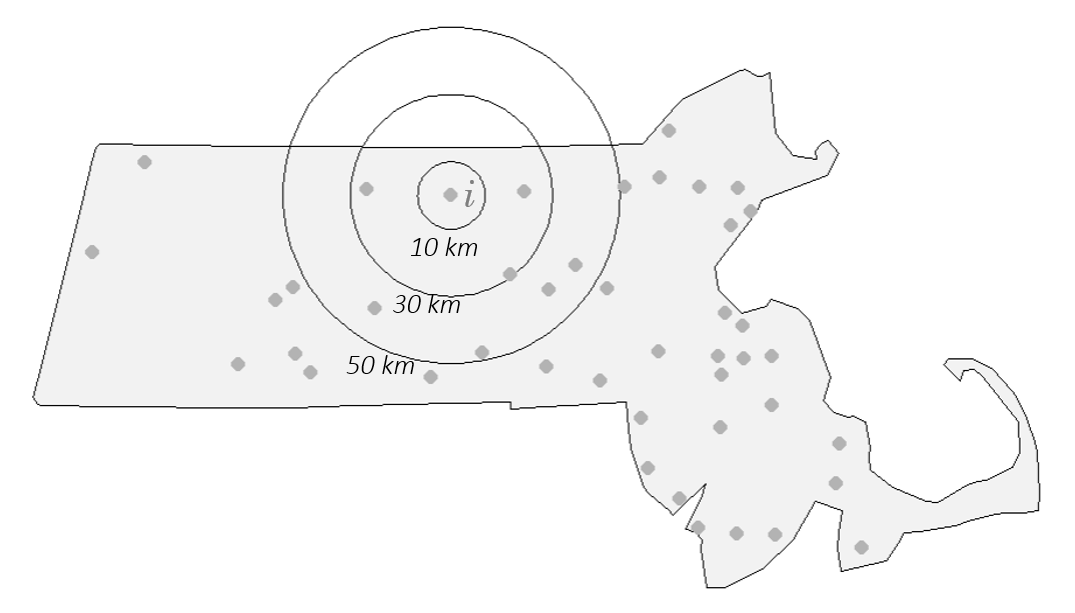
\includegraphics[width=4.6875in,height=\textheight,keepaspectratio]{img/K_bands.png}

}

\caption{\label{fig-K0}Illustration of how the K function summarizes the
number of points within a specified distance: Three concentric circles
are drawn around point \(i\), and the number of neighboring points
within each radius is tallied. In this example, no points fall within 10
km of \(i\), three points fall within 30 km, and seven points fall
within 50 km.}

\end{figure}%

Conceptually, the K function counts how many neighboring points fall
within a distance \(d\) of each point, averages this quantity over all
points in the pattern, and then adjusts the result for the overall point
density.

The estimator takes the form:

\[
\hat{K}(d) = \frac{A}{n(n-1)} \sum_{i=1}^{n} \sum_{j \neq i}^n I(d_{ij} \leq d)
\]

where:

\begin{itemize}
\tightlist
\item
  \(i\) refers to the reference point from which distances \(d\) are
  measured.
\item
  \(j\) refers to the other points in the pattern that are being
  evaluated to see whether they fall within a circle of radius \(d\)
  centered on \(i\).
\item
  \(d\) is the search distance for which we are counting neighboring
  points.
\item
  \(d_{ij}\) is the distance between point \(i\) and point \(j\).
\item
  \(I(d_{ij} \le d)\) is an indicator function that equals 1 if
  \(d_{ij} \le d\) and 0 otherwise.
\item
  \(\sum_{i=1}^{n}\) is the outer summation It means ``for each point
  \(i\) from the first point to the \(n\)\^{}th point, do the following
  \ldots{}''
\item
  \(\sum_{j \neq i}\) is the inner summation. For the current point
  \(i\) selected by the outer summation, sum the results of the
  indicator function over all points \(j\) in the dataset, excluding the
  case where \(j\) is the same as \(i\).
\item
  \(n(n-1)\) in the denominator is a normalizing factor. It represents
  the total number of ordered pairs of distinct points in the dataset.
  Dividing the total count from the double summation by \(n(n-1)\) gives
  the observed fraction of pairs separated by a distance less than or
  equal to \(d\).
\item
  \(A\) is the area of the study region. Multiplying the proportion by
  \(A\) scales the result into units of area, which makes comparison of
  the K function between datasets and theoretical K functions possible.
\end{itemize}

The units of the K function are units of area, typically defined by the
coordinate system of the point layer.

An equivalent and commonly encountered form of the estimator is:

\[ \widehat{K}(d) = \frac{1}{\widehat\lambda n} \sum_{i=1}^{n} \sum_{j \neq i} I(d_{ij} \leq d) \]
Although the notation appears more complicated than that of ANN, the
underlying idea is similar: the K function measures how many neighbors
occur within a given distance. The key difference is that K considers
\textbf{all neighbors within distance \(d\)}, whereas ANN focuses only
on the nearest (or n\textsuperscript{th}-nearest) neighbor.

Note that the intensity estimator used here,

\[
\hat{\lambda} = (n-1) / A
\]

is slightly different from the more intuitive ``natural'' estimator,

\[\hat{\lambda} = n/A\] that we used in Chapter 14. This difference is a
deliberate statistical adjustment related to the goal of the K function.
The K function characterizes a point pattern \textbf{from the
perspective of the events themselves}, focusing on the distances among
points. Think of it this way: when we stand at a particular event \(i\)
and count its neighbors, we are observing the density of the other
\((n-1)\) events within the study area \(A\).

\begin{figure}[H]

\centering{

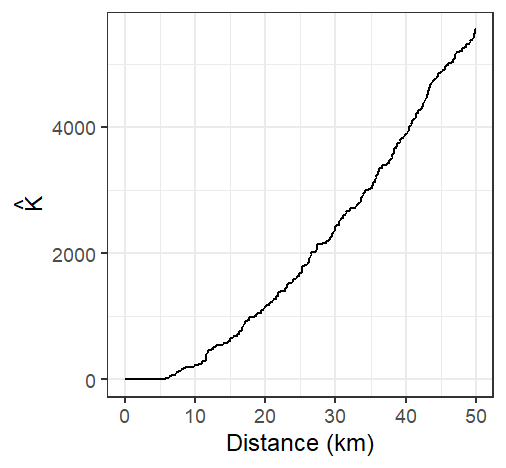
\includegraphics[width=3.64583in,height=\textheight,keepaspectratio]{img/K_function.png}

}

\caption{\label{fig-K1}The K function estimated from the Walmart stores
point distribution in MA for 512 distinct distances \(d\) ranging from 0
km to 50 km.}

\end{figure}%

A few important assumptions underlie the K function:

\begin{itemize}
\tightlist
\item
  The K function, as presented here, assumes a homogeneous first-order
  process because \(\hat{\lambda}\) is assumed to be constant throughout
  the study area.
\item
  The underlying process is assumed to be \textbf{isotropic}, meaning
  that spatial interaction depends on distance but not direction.
\item
  Because distances are central to the analysis, the coordinate system
  used with the point pattern should preserve distance unless geodesic
  distances are computed.
\end{itemize}

Like ANN, the K function can be sensitive to edge effects. Points near
the study area's boundary have fewer neighboring points available to be
counted, which can bias the K-function downward.

To reduce this bias, an edge correction is often applied to \(\hat{K}\).
A standard and widely used method applies an \textbf{isotropic
correction} weight that is the proportion of the \textbf{circumference}
of the circle centered on reference point \(i\) with radius \(d\) that
lies within the study area (e.g.~the state of Massachusetts in our
working example). The corrected K function estimator takes the form:

\[
\hat{K}(d) = \frac{A}{n(n-1)} \sum_{i=1}^{n} \sum_{j \neq i} \frac{I(d_{ij} \leq d)}{w_{ij}}
\]

where \(w_{ij}\) is the isotropic edge-correction weight, equal to the
proportion of the circumference of a circle centered on point \(i\) with
radius \(d\) that lies within the study area.

\begin{figure}[H]

\centering{

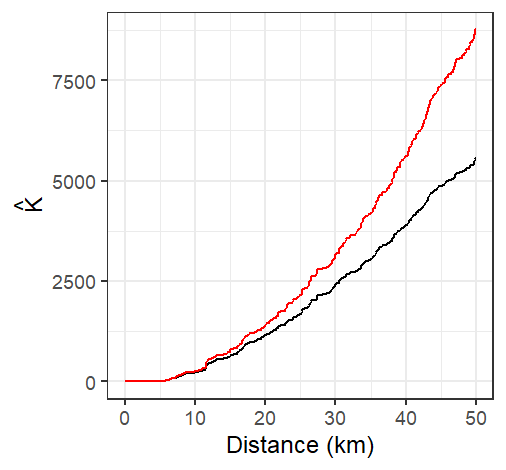
\includegraphics[width=3.64583in,height=\textheight,keepaspectratio]{img/K_function_iso.png}

}

\caption{\label{fig-K2}The K-function estimated from the Walmart stores
point distribution in MA (shown in black), and the isotropic edge
corrected K function for the same point layer (shown in red).}

\end{figure}%

Edge correction can substantially alter the interpretation of the K
function, particularly at larger distances where boundary effects become
more pronounced.

Under the assumption of \textbf{Complete Spatial Randomness (CSR)}, the
expected value of the K function is:

\[
K_{expected}(d) = \pi d^2
\]

This theoretical curve provides a benchmark against which the observed K
function can be compared.

\begin{itemize}
\tightlist
\item
  If the observed K function exceeds the CSR expectation, it suggests
  \textbf{clustering} at distance \(d\).
\item
  If the observed K function falls below the CSR expectation, it
  suggests \textbf{dispersion} at distance \(d\).
\item
  If the two functions are similar, the pattern is broadly consistent
  with CSR at that distance.
\end{itemize}

Conceptually, this comparison plays the same role as comparing an
observed ANN value to the ANN value expected under CSR.

\begin{figure}[H]

\centering{

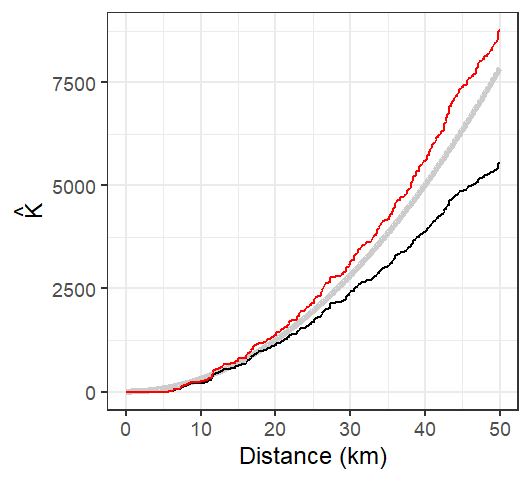
\includegraphics[width=3.64583in,height=\textheight,keepaspectratio]{img/K_function_iso_theo.png}

}

\caption{\label{fig-K3}The K-function estimated from the Walmart stores
point distribution in MA (shown in black), and the isotropic edge
corrected K function for the same point layer (shown in red). The thick
grey line represents the theoretical K function under the assumption of
Complete Spatial Randomness (CSR). Note how not correcting for edge
effect can mis-characterize the nature of the point pattern. The
uncorrected K function suggests a pattern more dispersed than expected
under CSR assumption for all distance values while the isotropic
weighted K function suggests clustering.}

\end{figure}%

\subsection{L function}\label{l-function}

One limitation of the K function is that it increases quadratically with
distance, making it difficult to visually assess small differences
between the observed K function and its expected value under Complete
Spatial Randomness (CSR). To address this issue, the \textbf{L function}
is often used as a variance-stabilizing transformation.

A common form of the L function is:

\[
L=\sqrt{\dfrac{K(d)}{\pi}}-d
\] Technically, the fundamental L function is written as

\[
L=\sqrt{\dfrac{K(d)}{\pi}}
\]

however, the \textbf{centered} form presented above has the advantage of
transforming the CSR expectation into a horizontal reference line at
zero. This makes departures from CSR easier to see across the full range
of distances.

Under CSR,

\[
L_{expected}(d) \approx 0
\]

Departures from zero indicate departures from randomness:

\begin{itemize}
\tightlist
\item
  \(L(d) > 0\): clustering at distance \(d\)
\item
  \(L(d) < 0\): dispersion at distance \(d\)
\end{itemize}

Conceptually, the L function contains the same information as the K
function but presents it in a form that is often easier to interpret
graphically.

\begin{figure}[H]

\centering{

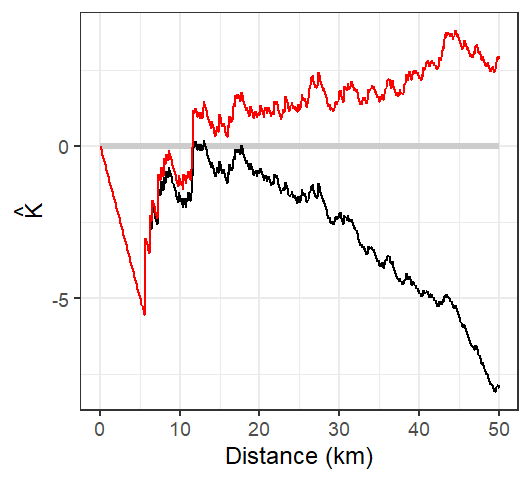
\includegraphics[width=3.64583in,height=\textheight,keepaspectratio]{img/L_function.png}

}

\caption{\label{fig-L}L function rendering of the K function. Both the
edge corrected (red line) and standard L functions (black line) are
shown. The theoretical L function under CSR is shown as a horizontal
line centered on 0.}

\end{figure}%

The L-function plot suggests that Walmart locations are more dispersed
than expected under CSR at distances up to approximately 12 km and more
clustered than expected at distances greater than 12 km.

\subsection{The Pair Correlation
Function}\label{the-pair-correlation-function}

While Ripley's K and L functions provide cumulative measures of spatial
dependence, the \textbf{Pair Correlation Function (PCF)} offers a more
localized, non-cumulative view of spatial structure. It is particularly
useful for identifying the specific distances at which clustering or
regularity occurs in a point pattern.

Recall that the K function counts all neighboring points up to a
distance \(d\). As a result, the influence of interactions occurring at
shorter distances carries forward into all larger distances. The Pair
Correlation Function avoids this accumulation and instead focuses on
interactions occurring at a specific distance.

The PCF, denoted \(g(d)\), describes the density of point pairs
separated by a distance \(d\), relative to what would be expected under
CSR. It is derived from the K function as:

\[
g(d) = \frac{1}{2\pi d}\frac{dK(d)}{dd}
\]

Here, \(\frac{dK(d)}{dd}\) denotes the first derivative of the K
function with respect to the distance \(d\), representing its
instantaneous rate of change. The notation \(dd\) in the denominator is
a single, indivisible symbol indicating differentiation with respect to
\(d\), and \emph{not} a product.

This formulation normalizes the rate of change in the cumulative K
function by the circumference of a ring at distance \(d\), yielding a
measure of point interaction at that specific scale.

\begin{itemize}
\tightlist
\item
  \(g(d) = 1\): The number of point pairs at distance \(d\) matches CSR
  expectations.
\item
  \(g(d) > 1\): More point pairs than expected at distance \(d\),
  suggesting \textbf{clustering}.
\item
  \(g(d) < 1\): Fewer point pairs than expected at distance \(d\),
  suggesting \textbf{dispersion}.
\end{itemize}

\begin{figure}[H]

\centering{


\includegraphics[width=6.77083in,height=\textheight,keepaspectratio]{img/K_vs_g_bands.png}

}

\caption{\label{fig-k_g}Difference in how the \(K\) and \(g\) functions
aggregate points at distance \(d\) (\(d\) = 30 km in this example).
\emph{All} points \emph{up to} \(d\) contribute to \(K\) whereas just
the points in the \emph{annulus band} at \(d\) contribute to \(g\).}

\end{figure}%

Like the K function from which it is derived, the pair correlation
function is susceptible to edge effects. Points located near the study
area's boundary have incomplete neighborhoods, leading to an
underestimation of point interactions at some distances. Because
\(g(d)\) is derived from the K function, any edge-related bias in the K
function will propagate to the PCF. Consequently, edge-correction
methods or guard areas are often used to obtain more reliable estimates,
particularly at larger distances.

Conceptually, the PCF plays a role similar to that of the L function,
but it focuses on interactions occurring at specific distances rather
than cumulative interactions across all shorter distances.

The plot of the pair correlation function for the Walmart store
locations is shown below. Both the edge-corrected and uncorrected
estimates are displayed for comparison.

\begin{figure}[H]

\centering{

\includegraphics[width=3.125in,height=\textheight,keepaspectratio]{img/g_function.png}

}

\caption{\label{fig-g}Estimated \(g\) function of the Massachusetts
Walmart point data. Its interpretation is similar to that of the \(K\)
function. Here, we observe distances between stores greater than
expected under CSR up to about 5 km. Note that this cutoff is shorter
than the 12 km threshold observed with the \(K\) function. The edge
uncorrected \(g\) function is depicted by a black line, while the
corrected \(g\) function is shown in a red line.}

\end{figure}%

The analysis of the \(g\) function suggests that Walmart stores exhibit
greater clustering than expected at distances exceeding approximately 5
kilometers. Recall that this threshold is shorter than the 12-kilometer
transition identified by the L function. This difference reflects the
localized nature of the pair correlation function: whereas the K and L
functions summarize interactions cumulatively across distances, the PCF
isolates interactions occurring at specific distances.

Like its \(K\), \(L\) and ANN counterparts, the \(g\)-function assumes
\emph{stationarity} and \emph{isotropy} in the underlying point process.

\subsection{Monte Carlo Tests for the K and L
Functions}\label{monte-carlo-tests-for-the-k-and-l-functions}

The Monte Carlo framework introduced earlier is not unique to Average
Nearest Neighbor analysis. It can be applied to many point pattern
statistics, including the K and L functions. The underlying logic
remains unchanged: a null model is specified, many realizations of that
model are simulated, and the observed statistic is compared to the
distribution of simulated statistics.

Unlike ANN, however, the K and L functions are evaluated at many
distance values \(d\). As a result, the Monte Carlo procedure generates
not a single sampling distribution, but a separate distribution for
every distance considered. Because displaying all of these distributions
simultaneously is impractical, the results are usually summarized using
simulation \emph{envelopes} superimposed on the observed K or L
function.

To construct a 95\% simulation envelope, the smallest and largest 2.5\%
of simulated values are removed for each distance \(d\). The remaining
values define the upper and lower bounds of the envelope. Because this
procedure is performed independently at each distance, such envelopes
are often referred to as \textbf{pointwise envelopes}.

The resulting envelope often exhibits a ``saw-tooth'' appearance because
the upper and lower limits are derived from a finite number of simulated
realizations at each distance.

\begin{figure}[H]

\centering{

\includegraphics[width=6.77083in,height=\textheight,keepaspectratio]{img/K_MC_sim_results_CSR.png}

}

\caption{\label{fig-k_l_mc_irp}Simulation results for the CSR
hypothesized process. The yellow line shows the edge corrected L
function. The gray envelope in the plot covers the 95\% significance
level. If the observed L lies outside of this envelope at distance
\(d\), then there is less than a 5\% chance that our observed point
pattern resulted from the simulated process at that distance.}

\end{figure}%

The interpretation of these plots follows the same logic as the ANN
Monte Carlo test. If \(\hat K\) or \(\hat L\) lies outside the
simulation envelope at distance \(d\), then the observed pattern may not
be consistent with the hypothesized process \(H_o\) at that distance. In
this example, the envelope represents a 95\% acceptance interval,
meaning that departures beyond the envelope are unlikely to occur if the
null model were true.

As with ANN analysis, the K and L functions assume a homogeneous
underlying process. If there is reason to believe that intensity varies
across space, then the analysis should be adjusted to account for this
inhomogeneity. For example, we might hypothesize that population density
influences the distribution of Walmart stores. In that case, Monte Carlo
simulations can be generated using the population density surface as the
underlying intensity function, producing an inhomogeneous null model.

\begin{figure}[H]

\centering{

\includegraphics[width=6.77083in,height=\textheight,keepaspectratio]{img/K_MC_sim_results_inhomogeneous.png}

}

\caption{\label{fig-k_l_mc_inhom}The L-function plot and simulation
results for an inhomogeneous hypothesized process. When controlled for
population density, the significance test suggests that the
inter-distance of Walmarts is more dispersed than expected under the
null up to a distance of 30 km.}

\end{figure}%

It may be tempting to scan a K- or L-function plot with pointwise
envelopes, identify distances where the observed function falls outside
the envelope, and report those distances as statistically significant.
However, this approach can be misleading. For example, based on the
results in the previous figure, we might be inclined to conclude that
the pattern is more dispersed than expected between distances of 5 and
30 kilometers at the \emph{5\% significance level}. In reality, this
interpretation can be misleading because many significance tests are
being performed simultaneously, one for each distance value. This issue,
known as the
\href{https://en.wikipedia.org/wiki/Multiple_comparisons_problem}{multiple
comparison problem}, is a statistical concern that arises when testing
many hypotheses simultaneously.

Global envelopes address this issue by providing a single significance
test across the entire range of distances, allowing departures from the
null model to be evaluated without inflating the probability of false
positives.

\subsection{Hypothesis Tests for the Pair Correlation
Function}\label{hypothesis-tests-for-the-pair-correlation-function}

Monte Carlo simulation techniques can be applied to the Pair Correlation
Function \(g(d)\) in exactly the same way they are applied to ANN, K,
and L functions. A hypothesized process is specified, many realizations
of that process are simulated, and a \(g(d)\) function is computed for
each realization.

Because \(g(d)\) is evaluated across many distance values \(d\), the
simulation results are typically summarized using simulation envelopes.
These envelopes represent the range of \(g(d)\) values expected under
the hypothesized process at each distance. If the observed \(g(d)\)
curve falls outside the envelope at some distance, this suggests that
the observed pattern may not be consistent with the hypothesized process
at that spatial scale.

As with the K and L functions, pointwise envelopes should be interpreted
cautiously because multiple distance values are being evaluated
simultaneously. This multiple-comparison problem can inflate the
probability of false positives. Global envelopes provide a more rigorous
alternative by offering a single significance assessment across the
entire range of distances.

\section{Summary}\label{summary-13}

This chapter introduced methods for analyzing second-order effects in
spatial point patterns. Whereas the previous chapter focused on how
point intensity varies across space (first-order effects), this chapter
examined how points are arranged relative to one another.

\begin{itemize}
\item
  \textbf{Second-order effects} describe how points are positioned
  relative to one another and whether they exhibit clustering or
  dispersion.
\item
  \textbf{Average Nearest Neighbor (ANN)} provides a simple measure of
  spatial interaction based on distances between neighboring points.
\item
  \textbf{Complete Spatial Randomness (CSR)} serves as a common null
  model against which observed point patterns can be compared.
\item
  \textbf{Monte Carlo tests} assess whether an observed pattern is
  consistent with a hypothesized process by comparing the observed
  statistic to simulated realizations of that process.
\item
  A hypothesis test does not identify the true generating process; it
  only evaluates whether the observed pattern is consistent with a
  specified hypothesis. Multiple competing hypotheses may therefore
  remain plausible.
\item
  Because first-order effects can create the appearance of clustering or
  dispersion, second-order analyses often require controlling for
  spatial variation in intensity.
\item
  \textbf{Ripley's K function}, \textbf{L function}, and the
  \textbf{Pair Correlation Function (PCF)} provide alternative summaries
  of spatial interaction across multiple spatial scales.
\item
  The same inferential framework used for ANN applies to K, L, and PCF
  analyses through Monte Carlo simulation and hypothesis testing.
\item
  No single statistic fully characterizes a point pattern. ANN, K, L,
  and PCF should be viewed as complementary tools for investigating
  spatial interaction.
\item
  Together with the first-order methods introduced in Chapter 14, these
  techniques provide a framework for understanding both the intensity of
  a point process and the interactions among its events
\end{itemize}

\chapter{Spatial Interpolation}\label{spatial-interpolation}

\section{Introduction}\label{introduction-15}

Given a distribution of meteorological stations reporting precipitation
values, how can we estimate precipitation at locations where no
observations were collected?

\begin{figure}[H]

\centering{

\pandocbounded{\includegraphics[keepaspectratio]{16_interpolation_files/figure-pdf/fig-precip_map-1.pdf}}

}

\caption{\label{fig-precip_map}Average yearly precipitation (reported in
inches) for several meteorological sites in Texas.}

\end{figure}%

To answer this question, we first need to clarify the nature of our
point dataset. In Chapters 14 and 15, we worked with point data
representing a complete enumeration of discrete events or observations.
In those cases, the phenomenon of interest existed only at the observed
point locations and could therefore only be measured at those locations.
For example, when mapping the density of retail stores or crime
incidents, the points themselves represent the complete set of observed
events.

Here, however, the point data represent \textbf{samples} of an
underlying phenomenon that can be measured \emph{anywhere} within our
study area. Precipitation is not limited to the locations of
meteorological stations; the stations merely provide observations of a
continuous environmental field. Consequently, creating a point-density
map from these data would only answer a question such as ``\emph{Where
are the meteorological stations concentrated within Texas?}'' rather
than ``\emph{How does precipitation vary across Texas?}''

To estimate values at unsampled locations, we use \textbf{spatial
interpolation} methods. Interpolation techniques use the values observed
at sampled locations to predict values elsewhere in the study area,
thereby transforming a set of discrete sample points into a continuous
surface.

Many interpolation methods exist, but most can be grouped into two broad
categories:

\begin{itemize}
\tightlist
\item
  \textbf{Deterministic interpolation}, which predicts values using
  mathematical rules based directly on the observed data.
\item
  \textbf{Statistical interpolation}, which incorporates an explicit
  statistical model of spatial variation and spatial dependence.
\end{itemize}

In the sections that follow, we examine representative methods from each
category and explore how their performance can be evaluated.

\section{Deterministic Approach to
Interpolation}\label{deterministic-approach-to-interpolation}

\textbf{Deterministic interpolation} methods estimate values at
unsampled locations using mathematical rules based directly on the
observed data. These methods do not explicitly model statistical
properties such as spatial autocorrelation or uncertainty. Instead, they
infer values using assumptions about the influence of nearby
observations.

In this section, we explore two deterministic methods:
\textbf{proximity} (also called \textbf{Thiessen}) interpolation and
\textbf{Inverse Distance Weighted (IDW)} interpolation.

\subsection{Proximity interpolation}\label{proximity-interpolation}

\textbf{Proximity interpolation} (also known as \textbf{Thiessen
interpolation}) is perhaps the simplest interpolation method and one of
the oldest. The idea is straightforward: every unsampled location is
assigned the value of its nearest sampled point.

This is accomplished by partitioning the study area into a set of
\emph{tessellated} regions. Boundaries are constructed midway between
neighboring sample locations, creating a set of polygons where every
location inside a polygon is closer to its enclosed sample point than to
any other sample point. Each polygon therefore inherits the value of its
sample point.

\begin{figure}[H]

\centering{

\pandocbounded{\includegraphics[keepaspectratio]{16_interpolation_files/figure-pdf/fig-proximity-1.pdf}}

}

\caption{\label{fig-proximity}Thiessen interpolation in which every
unsampled location inherits the value of the nearest sampled point. The
resulting tessellated surface is composed of polygons whose boundaries
are equidistant from neighboring sample locations.}

\end{figure}%

One limitation of this approach is that values change abruptly across
polygon boundaries. As a result, the interpolated surface is
discontinuous, whereas most environmental variables such as temperature,
elevation, and precipitation tend to vary more gradually across space.

Thiessen's method was particularly useful at a time when interpolation
had to be performed manually. Today, modern computing allows us to
implement more sophisticated interpolation techniques that produce
smoother surfaces, one of which is introduced next.

\subsection{Inverse Distance Weighted
(IDW)}\label{inverse-distance-weighted-idw}

The \textbf{Inverse Distance Weighted (IDW)} method estimates values at
unsampled locations by computing a weighted average of nearby sampled
values. The underlying assumption is simple: observations that are
closer to an unsampled location should exert a greater influence on the
prediction than observations that are farther away.

The interpolated value at an unsampled location \(j\) is computed as:

\[
\hat{Z_j} = \frac{\sum_i{Z_i/d^n_{ij}}}{\sum_i{1/d^n_{ij}}}
\] where:

\begin{itemize}
\tightlist
\item
  \(\hat{Z_j}\) is the predicted value at location \(j\),
\item
  \(Z_i\) is the observed value at sampled location \(i\),
\item
  \(d_{ij}\) is the distance between locations \(i\) and \(j\),
\item
  \(n\) is the \textbf{power coefficient}, which controls how quickly a
  point's influence decreases with distance.
\end{itemize}

The hat, \(\hat{}\), above the variable \(z\) indicates that the value
is being estimated rather than directly observed.

The power coefficient \(n\) controls the relative importance of nearby
and distant observations. Larger values of \(n\) cause the influence of
distant points to decrease rapidly, giving nearby points much greater
control over the prediction. As \(n\) becomes very large, the resulting
surface begins to resemble a Thiessen interpolation because the
prediction is dominated by the closest sample point.

Conversely, smaller values of \(n\) reduce the differences among the
weights assigned to neighboring points. In the extreme case where all
points receive similar weights, the interpolated value approaches the
average of the nearby observations.

The following figure shows an IDW interpolation generated using a power
coefficient of \(n=2\). The sampled precipitation values are
superimposed on the interpolated raster.

\begin{figure}[H]

\centering{

\pandocbounded{\includegraphics[keepaspectratio]{16_interpolation_files/figure-pdf/fig-idw1-1.pdf}}

}

\caption{\label{fig-idw1}An IDW interpolation of the average yearly
precipitation (reported in inches) for several meteorological sites in
Texas. An IDW power coefficient of 2 was used in this example.}

\end{figure}%

The power coefficient controls how rapidly the influence of a sampled
point decreases with distance from the prediction location. In the
following example, an \(n\) value of \(15\) is used. Relative to the
previous interpolation, nearby points exert much stronger influence on
the predicted values, whereas distant points have very little impact. As
a result, the interpolated surface begins to resemble a proximity
(Thiessen) interpolation, with localized zones of influence surrounding
the sampled points.

\begin{figure}[H]

\centering{

\pandocbounded{\includegraphics[keepaspectratio]{16_interpolation_files/figure-pdf/fig-idw2-1.pdf}}

}

\caption{\label{fig-idw2}An IDW interpolation of the average yearly
precipitation (reported in inches) for several meteorological sites in
Texas. An IDW power coefficient of 15 was used in this example.}

\end{figure}%

\subsection{Evaluating Interpolation
Accuracy}\label{evaluating-interpolation-accuracy}

Selecting the best interpolation parameters can be challenging. Beyond
simply \emph{eyeballing} the results, how can we quantify the
\emph{accuracy} of an interpolated surface? One approach is to divide
the sample points into two groups: a \textbf{training} set used to
generate the interpolation and a \textbf{validation} set used to assess
its performance. While straightforward to implement, this approach
reduces the amount of information available to the interpolator and can
therefore lead to less reliable estimates.

A more efficient approach is to temporarily remove one point from the
dataset, interpolate its value using all remaining points, and then
compare the predicted value to the observed value at the omitted
location. This process is repeated for every point in the dataset while
keeping the interpolation parameters fixed. The procedure is commonly
known as \textbf{jackknifing} or \textbf{leave-one-out
cross-validation}.

The performance of the interpolator can be summarized using the
\textbf{Root Mean Squared Error (RMSE)}:

\[
RMSE = \sqrt{\frac{\sum_{i=1}^n (\hat {Z_{i}} - Z_i)^2}{n}}
\]

where \(\hat {Z_{i}}\) is the interpolated value at the unsampled
location \emph{i} (i.e.~location where the sample point was removed),
\(Z_i\) is the true value at location \emph{i} and \(n\) is the number
of points in the dataset.

We can visualize the results by plotting the predicted values against
the observed values. The solid diagonal line represents perfect
agreement between predicted and observed values. If the interpolator
were perfectly accurate, all points would fall on this line. The red
dashed line is a fitted regression line included to help visualize the
overall pattern of agreement.

\begin{figure}[H]

\centering{

\pandocbounded{\includegraphics[keepaspectratio]{16_interpolation_files/figure-pdf/fig-rmse_plot-1.pdf}}

}

\caption{\label{fig-rmse_plot}Scatter plot comparing predicted and
observed precipitation values following leave-one-out cross-validation.
Points closer to the one-to-one line indicate better agreement between
interpolated and observed values.}

\end{figure}%

The computed RMSE from the above working example is 6.989 inches.

We can further evaluate interpolation uncertainty by creating a
confidence-interval map. This involves generating all \(n\)
leave-one-out interpolation surfaces and computing a confidence interval
for each raster cell.

Locations whose predicted values vary substantially across the
leave-one-out realizations will have larger confidence intervals,
indicating greater uncertainty. Conversely, locations whose predicted
values remain relatively stable across the realizations will have
smaller confidence intervals, indicating greater confidence in the
prediction.

The following map shows the 95\% confidence interval associated with
each location in the study area.

\begin{figure}[H]

\centering{

\pandocbounded{\includegraphics[keepaspectratio]{16_interpolation_files/figure-pdf/fig-confidence_map-1.pdf}}

}

\caption{\label{fig-confidence_map}Spatial distribution of interpolation
uncertainty derived from leave-one-out cross-validation. Areas with
larger confidence intervals are more sensitive to the omission of
individual sample points and therefore have greater uncertainty in their
predicted values.}

\end{figure}%

IDW is one of the most widely used interpolation methods because of its
simplicity and ease of implementation. In many situations it produces
reasonable results. However, the choice of power coefficient remains
somewhat subjective and the method does not explicitly model the spatial
structure of the data.

A second class of interpolation methods incorporates information about
large-scale spatial trends (first-order effects) and spatial
autocorrelation (second-order effects). These statistically based
approaches, introduced next, provide a more rigorous framework for
interpolation.

\section{Statistical Approach to
Interpolation}\label{statistical-approach-to-interpolation}

Unlike deterministic methods, which rely on predefined mathematical
rules, \textbf{statistical interpolation} methods use models to
characterize spatial variation in the observed data. These methods can
incorporate information about large-scale spatial trends
(\textbf{first-order effects}) as well as spatial autocorrelation
(\textbf{second-order effects}) when estimating values at unsampled
locations.

In this section, we explore two examples of statistical interpolation:
\textbf{surface trend} and \textbf{Kriging}.

\subsection{Trend Surfaces}\label{trend-surfaces}

A trend surface models how an attribute varies as a function of spatial
location. You can think of trend surface modeling as a regression in
which the predictor variables are the spatial coordinates \(X\) and
\(Y\). The resulting model is then used to estimate values at unsampled
locations.

Trend surfaces describe broad, large-scale variation across a study area
and therefore capture what we previously referred to as a
\textbf{first-order effect}. In Chapter 12, trend surfaces were
introduced as a tool for characterizing spatial trends in continuous
fields. Here, we revisit them as an interpolation method that can be
used to predict values at unsampled locations.

We will explore three trend surface models of increasing complexity: a
\textbf{0th-order}, \textbf{1st-order}, and \textbf{2nd-order} trend
surface.

\textbf{0\textsuperscript{th} Order Trend Surface}

The simplest possible trend surface assumes that the attribute being
modeled does not vary across space. In this case, every unsampled
location is assigned the same value: the mean of the observed sample
values. The model takes the form: \[
Z = a
\]

where \(a\) is the mean precipitation value of all sample points (27.1
inches in our working example). This model produces a perfectly flat
(horizontal) surface in which every location is assigned the same
precipitation value.

\begin{figure}[H]

\centering{

\pandocbounded{\includegraphics[keepaspectratio]{16_interpolation_files/figure-pdf/fig-poly0-1.pdf}}

}

\caption{\label{fig-poly0}The simplest model where all interpolated
surface values are equal to the mean precipitation, 27.09 in.}

\end{figure}%

Because all spatial variation is ignored, the resulting map is generally
uninformative. Nevertheless, the 0\textsuperscript{th}-order trend
surface provides a useful baseline against which more complex trend
surface models can be compared. In the next example, we allow the
surface to vary as a function of location, producing a
1\textsuperscript{st}-order trend surface.

\textbf{1\textsuperscript{st} Order Trend Surface}

A 1\textsuperscript{st}-order trend surface allows the interpolated
value to vary as a linear function of spatial location. The resulting
surface is a tilted plane whose slope and orientation are determined by
the fitted coefficients. The model takes the form:

\[
Z = a + bX + cY
\] where \(X\) and \(Y\) are the spatial coordinates and \(a\), \(b\),
and \(c\) are coefficients estimated from the observed data.

\begin{figure}[H]

\centering{

\pandocbounded{\includegraphics[keepaspectratio]{16_interpolation_files/figure-pdf/fig-poly1-1.pdf}}

}

\caption{\label{fig-poly1}Result of a first order interpolation.}

\end{figure}%

Unlike the 0\textsuperscript{th}-order model, which assigns the same
value everywhere, the 1\textsuperscript{st}-order trend surface captures
broad spatial variation across the study area. In this example, the
model highlights a pronounced east-west precipitation gradient.

However, a tilted plane assumes that the rate of change is constant
across the entire study area. Is the precipitation trend truly uniform
from east to west? To allow for curvature in the trend surface, we next
consider a more flexible model: the 2\textsuperscript{nd}-order
(quadratic) trend surface.

\textbf{2\textsuperscript{nd} Order Trend Surface}

A 2\textsuperscript{nd}-order trend surface extends the
1\textsuperscript{st}-order model by allowing the rate of change to vary
across space. The resulting surface is no longer a tilted plane but can
bend and curve to accommodate more complex spatial patterns. The model
takes the form:

\[
Z = a + bX + cY + dX^2 + eY^2 + fXY
\] where the quadratic terms (\(X^2\) and \(Y^2\)) and the interaction
term (\(XY\)) allow the surface to capture curvature and changes in
slope across the study area.

\begin{figure}[H]

\centering{

\pandocbounded{\includegraphics[keepaspectratio]{16_interpolation_files/figure-pdf/fig-poly2-1.pdf}}

}

\caption{\label{fig-poly2}Result of a second order interpolation.}

\end{figure}%

Relative to the 1\textsuperscript{st}-order trend surface, this model
captures a slight curvature in the east-west precipitation gradient.
However, the improvement is modest, suggesting that the additional model
complexity may not be justified for this dataset.

As trend surface order increases, the fitted surface becomes more
flexible and can capture increasingly complex spatial patterns. However,
higher-order models also risk fitting noise in the sampled data rather
than meaningful spatial structure. In practice, it is often preferable
to use the simplest model that adequately characterizes the observed
trend.

\subsection{Ordinary Kriging}\label{ordinary-kriging}

Several forms of kriging interpolators exist: ordinary, universal and
simple just to name a few. In this chapter, we focus on \textbf{ordinary
kriging} (\textbf{OK}), one of the most widely used geostatistical
interpolation methods.

Unlike deterministic interpolators such as Thiessen interpolation and
IDW, which rely on predefined distance-based rules, ordinary kriging
explicitly models the spatial structure of the data. In particular, it
uses information about \textbf{spatial autocorrelation} to determine how
much influence neighboring observations should have on an unsampled
location.

As discussed in previous chapters, spatial phenomena often exhibit both
\textbf{first-order effects} (large-scale spatial trends) and
\textbf{second-order effects} (spatial autocorrelation). The final
interpolation incorporates information from both first-order effects
(through the trend model) and second-order effects (through the
variogram and kriging interpolation).

The ordinary kriging workflow typically involves five steps:

\begin{itemize}
\tightlist
\item
  Removing any \textbf{spatial trend} in the data (if present).
\item
  Computing the \textbf{experimental variogram}, \(\gamma\), which
  quantifies spatial autocorrelation.
\item
  Defining a \textbf{variogram model} that characterizes the spatial
  autocorrelation structure.
\item
  Interpolating the residual surface using the variogram model.
\item
  Adding the interpolated residual surface back to the trend surface to
  produce the final prediction map.
\end{itemize}

These steps are outlined in the following subsections.

\subsubsection{De-trending the data}\label{de-trending-the-data}

One assumption underlying ordinary kriging is that the mean and variance
of the phenomenon being studied remain constant across the study area.
In other words, the data should not exhibit a spatial trend (sometimes
referred to as \textbf{drift} in the geostatistics literature) across
its studied extent.

As discussed earlier in this chapter, trend surfaces provide a
convenient way to model broad spatial variation. Many software packages
allow the user to fit and remove a trend surface, typically using a
first-, second-, or third-order polynomial. In our example, we use the
1st-order trend surface because the 2nd-order model provided only a
modest improvement over the simpler fit.

Removing the trend produces a set of \textbf{residuals}, which represent
the variation not explained by the large-scale spatial pattern. These
residuals are then used in the variogram and kriging calculations that
follow. Once the residual surface has been interpolated, the fitted
trend surface is added back to produce the final prediction map.

\begin{figure}[H]

\centering{

\pandocbounded{\includegraphics[keepaspectratio]{16_interpolation_files/figure-pdf/fig-detrend_map-1.pdf}}

}

\caption{\label{fig-detrend_map}Detrended precipitation residuals
obtained after removing the 1st-order trend surface. These residuals
represent local variation not explained by the large-scale east-west
precipitation gradient and form the input to the variogram analysis.}

\end{figure}%

\subsubsection{Experimental Variogram}\label{experimental-variogram}

The key idea behind kriging is that observations closer together in
space tend to be more similar than observations farther apart. To
quantify this relationship, we examine how differences between attribute
values change as the distance between sample locations increases.

We begin by computing a quantity called the semivariance, denoted by
\(\gamma\). Semivariance measures how different two observations are
from one another. Small values of \(gamma\) indicate that two locations
have similar attribute values, whereas large values indicate greater
dissimilarity.

For a pair of locations, semivariance is computed as:

\[
\gamma = \frac{(Z_2 - Z_1)^2}{2} 
\] where \(Z_1\) and \(Z_2\) are the attribute values observed at the
two locations.

For example, consider two meteorological stations whose detrended
precipitation values are -1.2 and 1.6.

\begin{figure}[H]

\centering{

\pandocbounded{\includegraphics[keepaspectratio]{16_interpolation_files/figure-pdf/fig-two_sites-1.pdf}}

}

\caption{\label{fig-two_sites}Locations of two sample sites used to
demonstrate the calculation of \emph{gamma}.}

\end{figure}%

Their semivariance is:

\[
\gamma = \frac{(-1.2 - (1.6))^2}{2} = 3.92
\]

We can repeat this calculation for every pair of sample locations in the
dataset. Plotting the resulting semivariance values against the
distances separating the corresponding point pairs produces the
following graph:

\begin{figure}[H]

\centering{

\pandocbounded{\includegraphics[keepaspectratio]{16_interpolation_files/figure-pdf/fig-variogram-1.pdf}}

}

\caption{\label{fig-variogram}Experimental variogram cloud of
precipitation residuals. Each point represents the semivariance
associated with a pair of sample locations, plotted against the distance
separating those locations. The red point corresponds to the pair
illustrated in Figure~\ref{fig-two_sites}}

\end{figure}%

The red point represents the semivariance computed in the previous
example. The corresponding pair of stations is separated by
approximately 209 km.

The above graph is called an \textbf{experimental variogram cloud} (or
\textbf{experimental semivariogram cloud}). The terms \emph{variogram}
and \emph{semivariogram} are commonly used interchangeably in
introductory geostatistics, and we will use the term \emph{variogram}
throughout the remainder of this chapter.

The word \emph{experimental} is important because the graph is
constructed from a sample of observations rather than from the complete
continuous field. Our goal in the next step is to use these sample-based
estimates to model the underlying spatial autocorrelation structure of
the precipitation field.

\subsubsection{Sample Experimental
Variogram}\label{sample-experimental-variogram}

Although the variogram cloud contains all pairwise semivariance
information, it can be difficult to interpret because of the large
number of point pairs. In our example, just 50 sample points generate
465 point pairs, even when considering only the first third of the
maximum lag distance.

A common way to simplify the variogram cloud is to group point pairs
into distance intervals called \textbf{lags}. The semivariance values
within each lag are then summarized, typically by computing their
average.

In the following example, the variogram cloud is divided into 15 lag
intervals. The average semivariance within each lag is shown as a red
point. These summary points are referred to as \textbf{sample
experimental variogram estimates}, and the resulting graph is called the
\textbf{sample experimental variogram}.

\begin{figure}[H]

\centering{

\pandocbounded{\includegraphics[keepaspectratio]{16_interpolation_files/figure-pdf/fig-sample_variogram-1.pdf}}

}

\caption{\label{fig-sample_variogram}Sample experimental variogram plot
of precipitation residual values.}

\end{figure}%

\subsubsection{Experimental Variogram
Model}\label{experimental-variogram-model}

The sample experimental variogram provides a useful summary of the
spatial autocorrelation present in the data. However, kriging requires a
smooth mathematical function from which semivariance values can be
predicted at any distance. We therefore fit a mathematical model to the
sample experimental variogram.

Many variogram models have been proposed, and the models available often
depend on the software being used. Examples of commonly used variogram
models are shown below.

\begin{figure}[H]

\centering{

\pandocbounded{\includegraphics[keepaspectratio]{16_interpolation_files/figure-pdf/fig-variogram_model-1.pdf}}

}

\caption{\label{fig-variogram_model}A subset of variogram models
available in R's \texttt{gstat} package.}

\end{figure}%

The goal is to identify the model that best describes the sample
experimental variogram. Most variogram models are characterized by
parameters that control the shape of the curve, including the
\textbf{nugget}, \textbf{range}, and \textbf{sill} (or \textbf{partial
sill}).

The following figure illustrates these parameters. The \textbf{nugget}
is the value where the variogram model intersects the y-axis. A non-zero
nugget implies that nearby observations are not perfectly identical,
which may reflect measurement error or variability occurring at scales
smaller than the sampling distance.

The \textbf{partial sill} is the vertical distance between the nugget
and the plateau of the variogram. If the nugget is zero, the partial
sill and sill are equivalent, and the term \textbf{sill} is typically
used. The \textbf{range} is the distance at which the variogram levels
off, indicating the distance beyond which observations are no longer
strongly spatially correlated.

\begin{figure}[H]

\centering{

\pandocbounded{\includegraphics[keepaspectratio]{16_interpolation_files/figure-pdf/fig-model_explained-1.pdf}}

}

\caption{\label{fig-model_explained}Graphical description of the range,
sill and nugget parameters in a variogram model.}

\end{figure}%

In our working example, we fit a \textbf{spherical variogram model}, one
of the most commonly used variogram models in geostatistics. Other
frequently used models include the \textbf{linear} and \textbf{Gaussian}
variogram models.

\begin{figure}[H]

\centering{

\pandocbounded{\includegraphics[keepaspectratio]{16_interpolation_files/figure-pdf/fig-spherical_model-1.pdf}}

}

\caption{\label{fig-spherical_model}A spherical model fit to our
residual variogram.}

\end{figure}%

\subsubsection{Kriging Interpolation}\label{kriging-interpolation}

The variogram model is used by the kriging interpolator to determine
\emph{localized} weighting parameters. Recall that in IDW interpolation,
the influence of neighboring points is controlled by a user-defined
power coefficient that is applied uniformly across the entire study
area. Every location therefore uses the same distance-decay rule.

Kriging takes a different approach. Instead of relying on a
user-specified power parameter, it uses the variogram model to determine
the weights assigned to neighboring observations. In effect, the
interpolation weights are derived from the observed spatial
autocorrelation structure of the data. Locations whose values have
historically exhibited stronger spatial dependence exert greater
influence on the prediction than locations exhibiting weaker dependence.

The mathematical implementation of kriging is considerably more involved
than that of IDW and will not be covered here. Conceptually, however,
kriging can be thought of as an interpolation method in which the data
themselves determine the weighting scheme through the variogram model.

The resulting interpolation of the residual surface is shown below.

\begin{figure}[H]

\centering{

\pandocbounded{\includegraphics[keepaspectratio]{16_interpolation_files/figure-pdf/fig-krige01-1.pdf}}

}

\caption{\label{fig-krige01}Kriged interpolation of the detrended
precipitation residuals. The surface represents local-scale variation
not explained by the broader precipitation trend.}

\end{figure}%

Recall that kriging was applied to the \textbf{detrended residuals}
rather than to the original precipitation values. Consequently, Figure
16.17 represents localized variation not explained by the large-scale
east-west trend. To generate the final precipitation map, the
interpolated residual surface is added back to the trend surface.

\begin{figure}[H]

\centering{

\pandocbounded{\includegraphics[keepaspectratio]{16_interpolation_files/figure-pdf/fig-krige02-1.pdf}}

}

\caption{\label{fig-krige02}The final kriged surface.}

\end{figure}%

A valuable by-product of kriging is a map of the \textbf{prediction
variance}, which provides a measure of uncertainty associated with the
interpolated values. Lower variance indicates greater confidence in the
prediction, whereas higher variance indicates greater uncertainty. Note
that variance is reported in squared units.

\begin{figure}[H]

\centering{

\pandocbounded{\includegraphics[keepaspectratio]{16_interpolation_files/figure-pdf/fig-krige03-1.pdf}}

}

\caption{\label{fig-krige03}Prediction variance map produced by the
kriging interpolation. Areas with larger variance indicate greater
uncertainty in the predicted precipitation values, whereas areas with
smaller variance indicate greater confidence in the prediction.}

\end{figure}%

\section{Summary}\label{summary-14}

Spatial interpolation estimates values at unsampled locations from point
observations that represent samples of a continuous field.

\begin{itemize}
\item
  Interpolation methods can be divided into two broad categories:
  \textbf{deterministic} and \textbf{statistical} approaches.
\item
  \textbf{Thiessen (proximity)} interpolation assigns each unsampled
  location the value of the nearest sampled point, producing a
  tessellated surface with abrupt boundaries.
\item
  \textbf{Inverse Distance Weighted (IDW)} interpolation predicts values
  using a weighted average of nearby observations, where closer points
  exert greater influence than distant points.
\item
  The accuracy of an interpolation can be evaluated using
  \textbf{leave-one-out cross-validation} (jackknifing), \textbf{RMSE},
  and maps of \textbf{interpolation uncertainty}.
\item
  \textbf{Trend surfaces} model broad spatial patterns using polynomial
  functions of spatial coordinates and can be used to interpolate values
  at unsampled locations.
\item
  \textbf{Ordinary kriging} differs from deterministic methods by
  explicitly incorporating information about spatial autocorrelation
  when determining interpolation weights. It involves removing
  large-scale trends, modeling spatial autocorrelation with a variogram,
  interpolating the residuals, and then adding the trend back to produce
  the final surface.
\item
  The \textbf{variogram} describes how similarity between observations
  changes with distance and forms the foundation of kriging
  interpolation.
\end{itemize}

\chapter*{References}\label{references}
\addcontentsline{toc}{chapter}{References}

\markboth{References}{References}

\protect\phantomsection\label{refs}
\begin{CSLReferences}{1}{1}
\bibitem[\citeproctext]{ref-Spatstat}
Baddeley, Adrian, Ege Rubak, and Rolf Turner. 2016. \emph{Spatial Point
Patterns, Methodology and Applications with r}. CRC Press.

\bibitem[\citeproctext]{ref-BaileyGatrell}
Bailey, Trevor C., and Anthony C. Gatrell. 1995. \emph{Interactive
Spatial Data Analysis}. Prentice Hall.

\bibitem[\citeproctext]{ref-spData}
Bivand, Roger, Jakub Nowosad, and Robin Lovelace. 2026. \emph{spData:
Datasets for Spatial Analysis}.
\url{https://doi.org/10.32614/CRAN.package.spData}.

\bibitem[\citeproctext]{ref-Wikle}
C. K. Wikle, N. Cressie, A. Zammit-Mangion. 2019. \emph{Spatio-Temporal
Statistics with r}. Chapman \& Hall/CRC.
\url{https://spacetimewithr.org/}.

\bibitem[\citeproctext]{ref-freedman1999ecological}
Freedman, David A. 1999. \emph{Ecological Inference and the Ecological
Fallacy}. Technical Report No. 549. University of California, Berkeley.
\url{https://statistics.berkeley.edu/sites/default/files/tech-reports/549.pdf}.

\bibitem[\citeproctext]{ref-spatial_data_analysis}
Haining, Robert. 2004. \emph{Spatial Data Analysis: Theory and
Practice}. Cambridge.

\bibitem[\citeproctext]{ref-Unwin1}
O'Sullivan, David, and David Unwin. 2010. \emph{Geographic Information
Analysis}. Wiley.

\bibitem[\citeproctext]{ref-openshaw1983maup}
Openshaw, Stan. 1983. {``The Modifiable Areal Unit Problem.''}
\emph{Concepts and Techniques in Modern Geography} 38.

\bibitem[\citeproctext]{ref-Pebesma_Bivand_SDS}
Pebesma, Edzer, and Roger Bivand. 2021. \emph{Spatial Data Science (with
Applications in r)}. \url{https://r-spatial.org/book/}.

\bibitem[\citeproctext]{ref-DataQuality2010}
Sun, M., and W. S. Wong. 2010. {``{Incorporating Data Quality
Information in Mapping American Community Survey Data}.''}
\emph{Cartography and Geography Information Science} 37 (4): 285--300.

\bibitem[\citeproctext]{ref-Tobler1970}
Tobler, Waldo R. 1970. {``{A Computer Movie Simulating Urban Growth in
the Detroit Region}.''} \emph{Economic Geography} 46 (2): 234--40.
\url{http://www.geog.ucsb.edu/~tobler/publications/pdf_docs/A-Computer-Movie.pdf}.

\bibitem[\citeproctext]{ref-DTomlin}
Tomlin, Dana C. 1990. \emph{GIS and Cartographic Modeling}. Prentice
Hall.

\bibitem[\citeproctext]{ref-Tukey1972}
Tukey, John W. 1972. \emph{{Some Graphic and Semigraphic Displays}}.
nos. August 1969: 293--316.

\bibitem[\citeproctext]{ref-Spatial_public_health}
Waller, Lance A., and Carol A. Gotway. 2004. \emph{Applied Spatial
Statistics for Public Health Data}. Wiley.

\end{CSLReferences}


\backmatter


\end{document}
